\documentclass[12pt,a4paper,twoside]{book}
\usepackage{minted}
\usepackage{graphicx}
\usepackage{setspace}	%double spacing for text, single for captions, footnotes, etc.
%\usepackage{hypernat} 	%substitut de cite que permet fer hyperlinks
\usepackage{natbib}		% substituye a 'hypernat' que funciona en Windows.
\usepackage[spanish]{babel}
\usepackage[utf8]{inputenc}
\usepackage{color}
\usepackage{hhline} 		% extended styles for tables
\usepackage{multirow}
\usepackage{subfigure}
\usepackage{acronym}
\usepackage{hyperref}
\usepackage{amsmath,amsmath,amssymb} 
\usepackage{fancyhdr}
\usepackage{epsfig, amsmath}
\usepackage{algorithm}
\usepackage{algorithmic}
\usepackage{pdfpages}
\usepackage{etoolbox} % we load it for the workaround

\usepackage[toc,page]{appendix}

\usepackage[section]{placeins}

\usepackage{etoolbox}
\makeatletter
\appto{\appendices}{\def\Hy@chapapp{Appendix}}
\makeatother



\renewcommand{\appendixtocname}{Apéndices}
\renewcommand{\appendixpagename}{Apéndices}




%%%%%JUPYTER
 \usepackage[Export]{adjustbox} % Used to constrain images to a maximum size
    \adjustboxset{max size={0.9\linewidth}{0.9\paperheight}}
     \usepackage[breakable]{tcolorbox}
    \usepackage{iftex}
    \ifPDFTeX
    	\usepackage[T1]{fontenc}

    \fi



    \AtBeginDocument{%
        \def\PYZsq{\textquotesingle}% Upright quotes in Pygmentized code
    }




    \usepackage{xcolor}
    \usepackage{geometry} 
    % Colors for the hyperref package
    \definecolor{urlcolor}{rgb}{0,.145,.698}
    \definecolor{linkcolor}{rgb}{.71,0.21,0.01}
    \definecolor{citecolor}{rgb}{.12,.54,.11}

    % ANSI colors
    \definecolor{ansi-black}{HTML}{3E424D}
    \definecolor{ansi-black-intense}{HTML}{282C36}
    \definecolor{ansi-red}{HTML}{E75C58}
    \definecolor{ansi-red-intense}{HTML}{B22B31}
    \definecolor{ansi-green}{HTML}{00A250}
    \definecolor{ansi-green-intense}{HTML}{007427}
    \definecolor{ansi-yellow}{HTML}{DDB62B}
    \definecolor{ansi-yellow-intense}{HTML}{B27D12}
    \definecolor{ansi-blue}{HTML}{208FFB}
    \definecolor{ansi-blue-intense}{HTML}{0065CA}
    \definecolor{ansi-magenta}{HTML}{D160C4}
    \definecolor{ansi-magenta-intense}{HTML}{A03196}
    \definecolor{ansi-cyan}{HTML}{60C6C8}
    \definecolor{ansi-cyan-intense}{HTML}{258F8F}
    \definecolor{ansi-white}{HTML}{C5C1B4}
    \definecolor{ansi-white-intense}{HTML}{A1A6B2}
    \definecolor{ansi-default-inverse-fg}{HTML}{FFFFFF}
    \definecolor{ansi-default-inverse-bg}{HTML}{000000}

    % commands and environments needed by pandoc snippets
    % extracted from the output of `pandoc -s`
%    \providecommand{\tightlist}{%
 %     \setlength{\itemsep}{0pt}\setlength{\parskip}{0pt}}
    \DefineVerbatimEnvironment{Highlighting}{Verbatim}{commandchars=\\\{\}}
    % Add ',fontsize=\small' for more characters per line
    \newenvironment{Shaded}{}{}
    \newcommand{\KeywordTok}[1]{\textcolor[rgb]{0.00,0.44,0.13}{\textbf{{#1}}}}
    \newcommand{\DataTypeTok}[1]{\textcolor[rgb]{0.56,0.13,0.00}{{#1}}}
    \newcommand{\DecValTok}[1]{\textcolor[rgb]{0.25,0.63,0.44}{{#1}}}
    \newcommand{\BaseNTok}[1]{\textcolor[rgb]{0.25,0.63,0.44}{{#1}}}
    \newcommand{\FloatTok}[1]{\textcolor[rgb]{0.25,0.63,0.44}{{#1}}}
    \newcommand{\CharTok}[1]{\textcolor[rgb]{0.25,0.44,0.63}{{#1}}}
    \newcommand{\StringTok}[1]{\textcolor[rgb]{0.25,0.44,0.63}{{#1}}}
    \newcommand{\CommentTok}[1]{\textcolor[rgb]{0.38,0.63,0.69}{\textit{{#1}}}}
    \newcommand{\OtherTok}[1]{\textcolor[rgb]{0.00,0.44,0.13}{{#1}}}
    \newcommand{\AlertTok}[1]{\textcolor[rgb]{1.00,0.00,0.00}{\textbf{{#1}}}}
    \newcommand{\FunctionTok}[1]{\textcolor[rgb]{0.02,0.16,0.49}{{#1}}}
    \newcommand{\RegionMarkerTok}[1]{{#1}}
    \newcommand{\ErrorTok}[1]{\textcolor[rgb]{1.00,0.00,0.00}{\textbf{{#1}}}}
    \newcommand{\NormalTok}[1]{{#1}}
    
    % Additional commands for more recent versions of Pandoc
    \newcommand{\ConstantTok}[1]{\textcolor[rgb]{0.53,0.00,0.00}{{#1}}}
    \newcommand{\SpecialCharTok}[1]{\textcolor[rgb]{0.25,0.44,0.63}{{#1}}}
    \newcommand{\VerbatimStringTok}[1]{\textcolor[rgb]{0.25,0.44,0.63}{{#1}}}
    \newcommand{\SpecialStringTok}[1]{\textcolor[rgb]{0.73,0.40,0.53}{{#1}}}
    \newcommand{\ImportTok}[1]{{#1}}
    \newcommand{\DocumentationTok}[1]{\textcolor[rgb]{0.73,0.13,0.13}{\textit{{#1}}}}
    \newcommand{\AnnotationTok}[1]{\textcolor[rgb]{0.38,0.63,0.69}{\textbf{\textit{{#1}}}}}
    \newcommand{\CommentVarTok}[1]{\textcolor[rgb]{0.38,0.63,0.69}{\textbf{\textit{{#1}}}}}
    \newcommand{\VariableTok}[1]{\textcolor[rgb]{0.10,0.09,0.49}{{#1}}}
    \newcommand{\ControlFlowTok}[1]{\textcolor[rgb]{0.00,0.44,0.13}{\textbf{{#1}}}}
    \newcommand{\OperatorTok}[1]{\textcolor[rgb]{0.40,0.40,0.40}{{#1}}}
    \newcommand{\BuiltInTok}[1]{{#1}}
    \newcommand{\ExtensionTok}[1]{{#1}}
    \newcommand{\PreprocessorTok}[1]{\textcolor[rgb]{0.74,0.48,0.00}{{#1}}}
    \newcommand{\AttributeTok}[1]{\textcolor[rgb]{0.49,0.56,0.16}{{#1}}}
    \newcommand{\InformationTok}[1]{\textcolor[rgb]{0.38,0.63,0.69}{\textbf{\textit{{#1}}}}}
    \newcommand{\WarningTok}[1]{\textcolor[rgb]{0.38,0.63,0.69}{\textbf{\textit{{#1}}}}}
    
    
    % Define a nice break command that doesn't care if a line doesn't already
    % exist.
    \def\br{\hspace*{\fill} \\* }
    % Math Jax compatibility definitions
    \def\gt{>}
    \def\lt{<}
    \let\Oldtex\TeX
    \let\Oldlatex\LaTeX
    \renewcommand{\TeX}{\textrm{\Oldtex}}
    \renewcommand{\LaTeX}{\textrm{\Oldlatex}}
    % Document parameters
    % Document title

    
    
    
    
    
% Pygments definitions
\makeatletter
\def\PY@reset{\let\PY@it=\relax \let\PY@bf=\relax%
    \let\PY@ul=\relax \let\PY@tc=\relax%
    \let\PY@bc=\relax \let\PY@ff=\relax}
\def\PY@tok#1{\csname PY@tok@#1\endcsname}
\def\PY@toks#1+{\ifx\relax#1\empty\else%
    \PY@tok{#1}\expandafter\PY@toks\fi}
\def\PY@do#1{\PY@bc{\PY@tc{\PY@ul{%
    \PY@it{\PY@bf{\PY@ff{#1}}}}}}}
\def\PY#1#2{\PY@reset\PY@toks#1+\relax+\PY@do{#2}}

\expandafter\def\csname PY@tok@w\endcsname{\def\PY@tc##1{\textcolor[rgb]{0.73,0.73,0.73}{##1}}}
\expandafter\def\csname PY@tok@c\endcsname{\let\PY@it=\textit\def\PY@tc##1{\textcolor[rgb]{0.25,0.50,0.50}{##1}}}
\expandafter\def\csname PY@tok@cp\endcsname{\def\PY@tc##1{\textcolor[rgb]{0.74,0.48,0.00}{##1}}}
\expandafter\def\csname PY@tok@k\endcsname{\let\PY@bf=\textbf\def\PY@tc##1{\textcolor[rgb]{0.00,0.50,0.00}{##1}}}
\expandafter\def\csname PY@tok@kp\endcsname{\def\PY@tc##1{\textcolor[rgb]{0.00,0.50,0.00}{##1}}}
\expandafter\def\csname PY@tok@kt\endcsname{\def\PY@tc##1{\textcolor[rgb]{0.69,0.00,0.25}{##1}}}
\expandafter\def\csname PY@tok@o\endcsname{\def\PY@tc##1{\textcolor[rgb]{0.40,0.40,0.40}{##1}}}
\expandafter\def\csname PY@tok@ow\endcsname{\let\PY@bf=\textbf\def\PY@tc##1{\textcolor[rgb]{0.67,0.13,1.00}{##1}}}
\expandafter\def\csname PY@tok@nb\endcsname{\def\PY@tc##1{\textcolor[rgb]{0.00,0.50,0.00}{##1}}}
\expandafter\def\csname PY@tok@nf\endcsname{\def\PY@tc##1{\textcolor[rgb]{0.00,0.00,1.00}{##1}}}
\expandafter\def\csname PY@tok@nc\endcsname{\let\PY@bf=\textbf\def\PY@tc##1{\textcolor[rgb]{0.00,0.00,1.00}{##1}}}
\expandafter\def\csname PY@tok@nn\endcsname{\let\PY@bf=\textbf\def\PY@tc##1{\textcolor[rgb]{0.00,0.00,1.00}{##1}}}
\expandafter\def\csname PY@tok@ne\endcsname{\let\PY@bf=\textbf\def\PY@tc##1{\textcolor[rgb]{0.82,0.25,0.23}{##1}}}
\expandafter\def\csname PY@tok@nv\endcsname{\def\PY@tc##1{\textcolor[rgb]{0.10,0.09,0.49}{##1}}}
\expandafter\def\csname PY@tok@no\endcsname{\def\PY@tc##1{\textcolor[rgb]{0.53,0.00,0.00}{##1}}}
\expandafter\def\csname PY@tok@nl\endcsname{\def\PY@tc##1{\textcolor[rgb]{0.63,0.63,0.00}{##1}}}
\expandafter\def\csname PY@tok@ni\endcsname{\let\PY@bf=\textbf\def\PY@tc##1{\textcolor[rgb]{0.60,0.60,0.60}{##1}}}
\expandafter\def\csname PY@tok@na\endcsname{\def\PY@tc##1{\textcolor[rgb]{0.49,0.56,0.16}{##1}}}
\expandafter\def\csname PY@tok@nt\endcsname{\let\PY@bf=\textbf\def\PY@tc##1{\textcolor[rgb]{0.00,0.50,0.00}{##1}}}
\expandafter\def\csname PY@tok@nd\endcsname{\def\PY@tc##1{\textcolor[rgb]{0.67,0.13,1.00}{##1}}}
\expandafter\def\csname PY@tok@s\endcsname{\def\PY@tc##1{\textcolor[rgb]{0.73,0.13,0.13}{##1}}}
\expandafter\def\csname PY@tok@sd\endcsname{\let\PY@it=\textit\def\PY@tc##1{\textcolor[rgb]{0.73,0.13,0.13}{##1}}}
\expandafter\def\csname PY@tok@si\endcsname{\let\PY@bf=\textbf\def\PY@tc##1{\textcolor[rgb]{0.73,0.40,0.53}{##1}}}
\expandafter\def\csname PY@tok@se\endcsname{\let\PY@bf=\textbf\def\PY@tc##1{\textcolor[rgb]{0.73,0.40,0.13}{##1}}}
\expandafter\def\csname PY@tok@sr\endcsname{\def\PY@tc##1{\textcolor[rgb]{0.73,0.40,0.53}{##1}}}
\expandafter\def\csname PY@tok@ss\endcsname{\def\PY@tc##1{\textcolor[rgb]{0.10,0.09,0.49}{##1}}}
\expandafter\def\csname PY@tok@sx\endcsname{\def\PY@tc##1{\textcolor[rgb]{0.00,0.50,0.00}{##1}}}
\expandafter\def\csname PY@tok@m\endcsname{\def\PY@tc##1{\textcolor[rgb]{0.40,0.40,0.40}{##1}}}
\expandafter\def\csname PY@tok@gh\endcsname{\let\PY@bf=\textbf\def\PY@tc##1{\textcolor[rgb]{0.00,0.00,0.50}{##1}}}
\expandafter\def\csname PY@tok@gu\endcsname{\let\PY@bf=\textbf\def\PY@tc##1{\textcolor[rgb]{0.50,0.00,0.50}{##1}}}
\expandafter\def\csname PY@tok@gd\endcsname{\def\PY@tc##1{\textcolor[rgb]{0.63,0.00,0.00}{##1}}}
\expandafter\def\csname PY@tok@gi\endcsname{\def\PY@tc##1{\textcolor[rgb]{0.00,0.63,0.00}{##1}}}
\expandafter\def\csname PY@tok@gr\endcsname{\def\PY@tc##1{\textcolor[rgb]{1.00,0.00,0.00}{##1}}}
\expandafter\def\csname PY@tok@ge\endcsname{\let\PY@it=\textit}
\expandafter\def\csname PY@tok@gs\endcsname{\let\PY@bf=\textbf}
\expandafter\def\csname PY@tok@gp\endcsname{\let\PY@bf=\textbf\def\PY@tc##1{\textcolor[rgb]{0.00,0.00,0.50}{##1}}}
\expandafter\def\csname PY@tok@go\endcsname{\def\PY@tc##1{\textcolor[rgb]{0.53,0.53,0.53}{##1}}}
\expandafter\def\csname PY@tok@gt\endcsname{\def\PY@tc##1{\textcolor[rgb]{0.00,0.27,0.87}{##1}}}
\expandafter\def\csname PY@tok@err\endcsname{\def\PY@bc##1{\setlength{\fboxsep}{0pt}\fcolorbox[rgb]{1.00,0.00,0.00}{1,1,1}{\strut ##1}}}
\expandafter\def\csname PY@tok@kc\endcsname{\let\PY@bf=\textbf\def\PY@tc##1{\textcolor[rgb]{0.00,0.50,0.00}{##1}}}
\expandafter\def\csname PY@tok@kd\endcsname{\let\PY@bf=\textbf\def\PY@tc##1{\textcolor[rgb]{0.00,0.50,0.00}{##1}}}
\expandafter\def\csname PY@tok@kn\endcsname{\let\PY@bf=\textbf\def\PY@tc##1{\textcolor[rgb]{0.00,0.50,0.00}{##1}}}
\expandafter\def\csname PY@tok@kr\endcsname{\let\PY@bf=\textbf\def\PY@tc##1{\textcolor[rgb]{0.00,0.50,0.00}{##1}}}
\expandafter\def\csname PY@tok@bp\endcsname{\def\PY@tc##1{\textcolor[rgb]{0.00,0.50,0.00}{##1}}}
\expandafter\def\csname PY@tok@fm\endcsname{\def\PY@tc##1{\textcolor[rgb]{0.00,0.00,1.00}{##1}}}
\expandafter\def\csname PY@tok@vc\endcsname{\def\PY@tc##1{\textcolor[rgb]{0.10,0.09,0.49}{##1}}}
\expandafter\def\csname PY@tok@vg\endcsname{\def\PY@tc##1{\textcolor[rgb]{0.10,0.09,0.49}{##1}}}
\expandafter\def\csname PY@tok@vi\endcsname{\def\PY@tc##1{\textcolor[rgb]{0.10,0.09,0.49}{##1}}}
\expandafter\def\csname PY@tok@vm\endcsname{\def\PY@tc##1{\textcolor[rgb]{0.10,0.09,0.49}{##1}}}
\expandafter\def\csname PY@tok@sa\endcsname{\def\PY@tc##1{\textcolor[rgb]{0.73,0.13,0.13}{##1}}}
\expandafter\def\csname PY@tok@sb\endcsname{\def\PY@tc##1{\textcolor[rgb]{0.73,0.13,0.13}{##1}}}
\expandafter\def\csname PY@tok@sc\endcsname{\def\PY@tc##1{\textcolor[rgb]{0.73,0.13,0.13}{##1}}}
\expandafter\def\csname PY@tok@dl\endcsname{\def\PY@tc##1{\textcolor[rgb]{0.73,0.13,0.13}{##1}}}
\expandafter\def\csname PY@tok@s2\endcsname{\def\PY@tc##1{\textcolor[rgb]{0.73,0.13,0.13}{##1}}}
\expandafter\def\csname PY@tok@sh\endcsname{\def\PY@tc##1{\textcolor[rgb]{0.73,0.13,0.13}{##1}}}
\expandafter\def\csname PY@tok@s1\endcsname{\def\PY@tc##1{\textcolor[rgb]{0.73,0.13,0.13}{##1}}}
\expandafter\def\csname PY@tok@mb\endcsname{\def\PY@tc##1{\textcolor[rgb]{0.40,0.40,0.40}{##1}}}
\expandafter\def\csname PY@tok@mf\endcsname{\def\PY@tc##1{\textcolor[rgb]{0.40,0.40,0.40}{##1}}}
\expandafter\def\csname PY@tok@mh\endcsname{\def\PY@tc##1{\textcolor[rgb]{0.40,0.40,0.40}{##1}}}
\expandafter\def\csname PY@tok@mi\endcsname{\def\PY@tc##1{\textcolor[rgb]{0.40,0.40,0.40}{##1}}}
\expandafter\def\csname PY@tok@il\endcsname{\def\PY@tc##1{\textcolor[rgb]{0.40,0.40,0.40}{##1}}}
\expandafter\def\csname PY@tok@mo\endcsname{\def\PY@tc##1{\textcolor[rgb]{0.40,0.40,0.40}{##1}}}
\expandafter\def\csname PY@tok@ch\endcsname{\let\PY@it=\textit\def\PY@tc##1{\textcolor[rgb]{0.25,0.50,0.50}{##1}}}
\expandafter\def\csname PY@tok@cm\endcsname{\let\PY@it=\textit\def\PY@tc##1{\textcolor[rgb]{0.25,0.50,0.50}{##1}}}
\expandafter\def\csname PY@tok@cpf\endcsname{\let\PY@it=\textit\def\PY@tc##1{\textcolor[rgb]{0.25,0.50,0.50}{##1}}}
\expandafter\def\csname PY@tok@c1\endcsname{\let\PY@it=\textit\def\PY@tc##1{\textcolor[rgb]{0.25,0.50,0.50}{##1}}}
\expandafter\def\csname PY@tok@cs\endcsname{\let\PY@it=\textit\def\PY@tc##1{\textcolor[rgb]{0.25,0.50,0.50}{##1}}}

\def\PYZbs{\char`\\}
\def\PYZus{\char`\_}
\def\PYZob{\char`\{}
\def\PYZcb{\char`\}}
\def\PYZca{\char`\^}
\def\PYZam{\char`\&}
\def\PYZlt{\char`\<}
\def\PYZgt{\char`\>}
\def\PYZsh{\char`\#}
\def\PYZpc{\char`\%}
\def\PYZdl{\char`\$}
\def\PYZhy{\char`\-}
\def\PYZsq{\char`\'}
\def\PYZdq{\char`\"}
\def\PYZti{\char`\~}
% for compatibility with earlier versions
\def\PYZat{@}
\def\PYZlb{[}
\def\PYZrb{]}
\makeatother


    % For linebreaks inside Verbatim environment from package fancyvrb. 
    \makeatletter
        \newbox\Wrappedcontinuationbox 
        \newbox\Wrappedvisiblespacebox 
        \newcommand*\Wrappedvisiblespace {\textcolor{red}{\textvisiblespace}} 
        \newcommand*\Wrappedcontinuationsymbol {\textcolor{red}{\llap{\tiny$\m@th\hookrightarrow$}}} 
        \newcommand*\Wrappedcontinuationindent {3ex } 
        \newcommand*\Wrappedafterbreak {\kern\Wrappedcontinuationindent\copy\Wrappedcontinuationbox} 
        % Take advantage of the already applied Pygments mark-up to insert 
        % potential linebreaks for TeX processing. 
        %        {, <, #, %, $, ' and ": go to next line. 
        %        _, }, ^, &, >, - and ~: stay at end of broken line. 
        % Use of \textquotesingle for straight quote. 
        \newcommand*\Wrappedbreaksatspecials {% 
            \def\PYGZus{\discretionary{\char`\_}{\Wrappedafterbreak}{\char`\_}}% 
            \def\PYGZob{\discretionary{}{\Wrappedafterbreak\char`\{}{\char`\{}}% 
            \def\PYGZcb{\discretionary{\char`\}}{\Wrappedafterbreak}{\char`\}}}% 
            \def\PYGZca{\discretionary{\char`\^}{\Wrappedafterbreak}{\char`\^}}% 
            \def\PYGZam{\discretionary{\char`\&}{\Wrappedafterbreak}{\char`\&}}% 
            \def\PYGZlt{\discretionary{}{\Wrappedafterbreak\char`\<}{\char`\<}}% 
            \def\PYGZgt{\discretionary{\char`\>}{\Wrappedafterbreak}{\char`\>}}% 
            \def\PYGZsh{\discretionary{}{\Wrappedafterbreak\char`\#}{\char`\#}}% 
            \def\PYGZpc{\discretionary{}{\Wrappedafterbreak\char`\%}{\char`\%}}% 
            \def\PYGZdl{\discretionary{}{\Wrappedafterbreak\char`\$}{\char`\$}}% 
            \def\PYGZhy{\discretionary{\char`\-}{\Wrappedafterbreak}{\char`\-}}% 
            \def\PYGZsq{\discretionary{}{\Wrappedafterbreak\textquotesingle}{\textquotesingle}}% 
            \def\PYGZdq{\discretionary{}{\Wrappedafterbreak\char`\"}{\char`\"}}% 
            \def\PYGZti{\discretionary{\char`\~}{\Wrappedafterbreak}{\char`\~}}% 
        } 
        % Some characters . , ; ? ! / are not pygmentized. 
        % This macro makes them "active" and they will insert potential linebreaks 
        \newcommand*\Wrappedbreaksatpunct {% 
            \lccode`\~`\.\lowercase{\def~}{\discretionary{\hbox{\char`\.}}{\Wrappedafterbreak}{\hbox{\char`\.}}}% 
            \lccode`\~`\,\lowercase{\def~}{\discretionary{\hbox{\char`\,}}{\Wrappedafterbreak}{\hbox{\char`\,}}}% 
            \lccode`\~`\;\lowercase{\def~}{\discretionary{\hbox{\char`\;}}{\Wrappedafterbreak}{\hbox{\char`\;}}}% 
            \lccode`\~`\:\lowercase{\def~}{\discretionary{\hbox{\char`\:}}{\Wrappedafterbreak}{\hbox{\char`\:}}}% 
            \lccode`\~`\?\lowercase{\def~}{\discretionary{\hbox{\char`\?}}{\Wrappedafterbreak}{\hbox{\char`\?}}}% 
            \lccode`\~`\!\lowercase{\def~}{\discretionary{\hbox{\char`\!}}{\Wrappedafterbreak}{\hbox{\char`\!}}}% 
            \lccode`\~`\/\lowercase{\def~}{\discretionary{\hbox{\char`\/}}{\Wrappedafterbreak}{\hbox{\char`\/}}}% 
            \catcode`\.\active
            \catcode`\,\active 
            \catcode`\;\active
            \catcode`\:\active
            \catcode`\?\active
            \catcode`\!\active
            \catcode`\/\active 
            \lccode`\~`\~ 	
        }
    \makeatother

    \let\OriginalVerbatim=\Verbatim
    \makeatletter
    \renewcommand{\Verbatim}[1][1]{%
        %\parskip\z@skip
        \sbox\Wrappedcontinuationbox {\Wrappedcontinuationsymbol}%
        \sbox\Wrappedvisiblespacebox {\FV@SetupFont\Wrappedvisiblespace}%
        \def\FancyVerbFormatLine ##1{\hsize\linewidth
            \vtop{\raggedright\hyphenpenalty\z@\exhyphenpenalty\z@
                \doublehyphendemerits\z@\finalhyphendemerits\z@
                \strut ##1\strut}%
        }%
        % If the linebreak is at a space, the latter will be displayed as visible
        % space at end of first line, and a continuation symbol starts next line.
        % Stretch/shrink are however usually zero for typewriter font.
        \def\FV@Space {%
            \nobreak\hskip\z@ plus\fontdimen3\font minus\fontdimen4\font
            \discretionary{\copy\Wrappedvisiblespacebox}{\Wrappedafterbreak}
            {\kern\fontdimen2\font}%
        }%
        
        % Allow breaks at special characters using \PYG... macros.
        \Wrappedbreaksatspecials
        % Breaks at punctuation characters . , ; ? ! and / need catcode=\active 	
        \OriginalVerbatim[#1,codes*=\Wrappedbreaksatpunct]%
    }
    \makeatother

    % Exact colors from NB
    \definecolor{incolor}{HTML}{303F9F}
    \definecolor{outcolor}{HTML}{D84315}
    \definecolor{cellborder}{HTML}{CFCFCF}
    \definecolor{cellbackground}{HTML}{F7F7F7}
    
    % prompt
    \makeatletter
    \newcommand{\boxspacing}{\kern\kvtcb@left@rule\kern\kvtcb@boxsep}
    \makeatother
    \newcommand{\prompt}[4]{
        \ttfamily\llap{{\color{#2}[#3]:\hspace{3pt}#4}}\vspace{-\baselineskip}
    }
    

    
    % Prevent overflowing lines due to hard-to-break entities
    \sloppy 
  
    % Slightly bigger margins than the latex defaults
    
    \geometry{verbose,tmargin=1in,bmargin=1in,lmargin=1in,rmargin=1in}





%%%%GENERAL




% general settings
\hypersetup{
	linktocpage=true,
	colorlinks=true,
	linkcolor=blue,
	citecolor=blue,
}
\definecolor{Hgray}{gray}{0.6}

\newenvironment{definition}[1][Definition]{\begin{trivlist}
\item[\hskip \labelsep {\bfseries #1}]}{\end{trivlist}}

\setlength{\topmargin}{0cm}
\setlength{\textheight}{23cm}
\setlength{\textwidth}{17cm}
\setlength{\oddsidemargin}{0cm}
\setlength{\evensidemargin}{0cm}
\setlength{\headheight}{1cm}

% indica que las 'sub-sub-sections' sean numeradas y aparezcan en el indice
\setcounter{secnumdepth}{3}
\setcounter{tocdepth}{2}

% settings for code
\renewcommand{\algorithmicrequire}{\textbf{Entrada: }}
\renewcommand{\algorithmicensure}{\textbf{Salida: }}





%%%%%%%%%%%%
% DOCUMENT %
%%%%%%%%%%%%
\begin{document}

% portada
\newpage
\thispagestyle{empty}

\baselineskip 2em

%\vspace*{1cm}

\centerline{
\includegraphics[width=0.6\textwidth]{images/UOC-logo}}
\begin{center}
\textsc{Universitat Oberta de Catalunya (UOC) \\
 Máster Universitario en Ciencia de Datos (\textit{Data Science})\\}

%\centerline {\pic{UOC}{4cm}}

\vspace*{1.5cm}

\textsc{\Large TRABAJO FINAL DE MÁSTER}

\vspace*{0.5cm}

\textsc{\large Área: PLN}


%\textbf{\Huge VirtualTechLab Model: }

\vspace*{2.0cm}

\textbf{\Large Modelización de temas de llamadas en tiempo real}

\textbf{\large PEC II}

\vspace{2.5cm}
\baselineskip 1em

\baselineskip 2em
-----------------------------------------------------------------------------\\
Autor:      Manuel E. Gómez Montero\\
Tutora UOC:      Ana Valdivia Garcia\\
Tutor TE:      Antonio Fernández Gallardo\\
Profesor:   Jordi Casas\\
-----------------------------------------------------------------------------\\
\vspace*{1.5cm}
Madrid, \today

\end{center}

\newpage
\pagestyle{empty}
\hfill

\newpage
% abstract
\pagenumbering{roman} 
\setcounter{page}{1} 
\pagestyle{plain}

%%%%%%%%%%%%%%%%
%%% CREDITOS %%%
%%%%%%%%%%%%%%%%
\chapter*{Créditos/Copyright}

%Una página con la especificación de créditos/copyright para el proyecto (ya sea aplicación por un lado y documentación por el otro, o unificadamente), así como la del uso de marcas, productos o servicios de terceros (incluidos códigos fuente). Si una persona diferente al autor colaboró en el proyecto, tiene que quedar explicitada su identidad y qué hizo.

%A continuación se ejemplifica el caso más habitual, aunque se puede modificar por cualquier otra alternativa:

\vspace{1cm}

\begin{figure}[ht]
    \centering
	
\includegraphics[scale=0.2]{images/license.png}
\end{figure}

Esta obra está sujeta a una licencia de Reconocimiento-CompartirIgual \href{https://creativecommons.org/licenses/by-sa/4.0/deed.es}{4.0 Internacional (CC BY-SA 4.0)}.

%%%%%%%%%%%%%
%%% FICHA %%%
%%%%%%%%%%%%%
\chapter*{FICHA DEL TRABAJO FINAL}

\begin{table}[ht]
	\centering{}
	\renewcommand{\arraystretch}{2}
	\begin{tabular}{r | l}
		\hline
		Título del trabajo: &  Modelización de temas de llamadas en tiempo real\\
		\hline
       Nombre del autor: & Manuel E. Gómez Montero\\
		\hline
        Tutor UOC: & Ana Valdivia Garcia\\
		\hline
		Tutor TME: & Antonio Fernández Gallardo\\
		\hline
        Nombre del PRA: & Jordi Casas Roma\\
		\hline
        Fecha de entrega (mm/aaaa): & 01/2019\\
		\hline
        Titulación o programa: & Máster Universitario en Ciencia de Datos\\
		\hline
        Área del Trabajo Final: & Procesamiento del Lenguaje Natural\\
		\hline
        Idioma del trabajo: & Español\\
		\hline
        Palabras clave & ``natural language processing'', ``sentiment analysis'',\\
        & ``real time'', ``call center'', ``topic modeling'', ``deep learning''\\
		\hline
	\end{tabular}
\end{table}

%%%%%%%%%%%%%%%%%%%
%%% DEDICATORIA %%%
%%%%%%%%%%%%%%%%%%%
%\chapter*{Dedicatoria/Cita}

%Breves palabras de dedicatoria y/o una cita.
\cleardoublepage
\begin{dedication}
A Ana, por el tiempo robado
\end{dedication}
\cleardoublepage
%%%%%%%%%%%%%%%%%%%
%%% Agradecimientos %%%
%%%%%%%%%%%%%%%%%%%
\chapter*{Agradecimientos}


Un \textit{handicap} a la hora de realizar el proyecto dentro de una gran empresa ha sido el hecho de trabajar con unos plazos tan ajustados. Aspectos como la autorización en el acceso a la información, el acceso a diferentes entornos, la intercomunicación entre áreas, etc. requieren unos tiempos que pueden retrasar la ejecución de un trabajo de este tipo. 
 
Este apartado tiene como objetivo agradecer a todas las personas que han hecho posible la realización de este proyecto en tiempo y forma.


A Willy Gavilán y Carolina Bouvard por hacer posible la  realización de este proyecto dentro de Telefónica. A Antonio Fernández por aceptar que realice este trabajo con su equipo y por tutorizarlo. A Jorge Ayuso y Rus Mesas por su ayuda a la hora de obtener los datos, por sus consejos y por permitirme usar con ellos el equipo con GPUs usados para  el entrenamiento y optimización de modelos. A Laura Canga por permitirme usar el Bus Apache Kafka y a José Ramón Fernández por ayudarme, incluso a deshoras, con la creación de \textit{topics} y usuarios del bus.  A Pablo Palomares por su ayuda a la hora de acceder y adaptar a nuestras necesidades las plataformas \textit{DevOps}: Bitbucket, Nexus y Jenkins. A Nacho Charfolé por darme su visión más allá de la parte técnica y por hacerme entender las ventajas que pueden aportar este tipo de proyectos a una empresa. Y por último, pero no menos importante, a mi tutora, Ana Valdivia, por sus correcciones minuciosas y por guiarme y animarme en todo momento.

Sin todos vosotros un trabajo de este tipo no sería posible. \textbf{{\LARGE Gracias}}.


%%%%%%%%%%%%%%%%
%%% RESUMEN  %%%
%%%%%%%%%%%%%%%%
\chapter*{Resumen}
\addcontentsline{toc}{chapter}{Resumen}


Un \textit{call center} es el área de una empresa el cuál se encarga de recibir y transmitir llamadas desde o hacia clientes, socios comerciales u otras compañías externas. La gran cantidad de información generada a partir de estas llamada refleja, entre otros aspectos, las necesidades de los clientes de la empresa. 


La capacidad de clasificar las llamadas recibidas en tiempo real en función de la temática , provocaría en las empresas una mejora en la calidad de atención al público y en la experiencia del cliente.  Esto es abordable mediante técnicas de \textit{machine learning}.

%Por ello, resulta una tarea esencial ser capaces de reaccionar en el menor tiempo posible ante un cambio en la temática de las llamadas con el objetivo de mejorar la experiencia del cliente.

%optimizar el tiempo de respuesta ante un cambio en la temática de las llamadas, para así reaccionar en tiempo real a las peticiones de los mismos y mejorar la percepción que estos tienen sobre la compañía. 

%Las empresas mejorarían la calidad de las llamadas de atención al público si fuesen capaces de clasificar en tiempo real las llamadas que reciben o emiten, en función de la temática que se este tratando en cada momento. Esto es abordable mediante técnicas de machine learning. 

En este documento se presenta un sistema implementado en el \textit{call center} de Telefónica que nos 
 permite, a partir de la transcripción de las llamadas, obtener la temática de las mismas utilizando métodos de Procesamiento de Lenguaje Natural. El análisis expuesto realiza clasificaciones con diferentes arquitecturas, tanto con modelos no supervisados como con modelos supervisados de aprendizaje profundo. Dependiendo del modelo se han estudiado también diferentes métodos a la hora de representar las transcripciones.
 
 Por último, se ha llevado uno de los modelos a producción, dotando al sistema de la posibilidad de realizar esta clasificación en tiempo real y proporcionando a la empresa la capacidad de visualizar la evolución de las llamadas a lo largo del tiempo y de generar alertas en base a anomalías. El sistema llevado a producción ha sido totalmente desplegado en contenedores y provisto de mecanismos  de monitorización, integración continua y despliegue continuo. 
 
El proyecto presentado abre a la empresa un gran número de posibilidades, tanto a la hora de  realizar nuevos sistemas de Procesamiento del Lenguaje Natural, como a la hora de llevar modelos de aprendizaje profundo a un entorno productivo.
 





%El documento que se presenta tiene como objetivo final mejorar la operatividad del \textit{call-center}  de una gran empresa, extrayendo mediante técnicas de \textit{machine learning} la temática de las llamadas que se realizan al mismo y dando la posibilidad a la empresa de reaccionar en tiempo real, en función de la temática que se este tratando en cada momento. 

%En este documento se presenta un sistema implementado en el \textit{call-center} de Telefónica que nos  permite, a partir de la transcripción de las llamadas, descubrir en tiempo real la temática de las mismas. Esta modelización de \textit{topics} se ha realizado utilizando métodos de Procesamiento de Lenguaje Natural y aprendizaje profundo. El sistema realiza la clasificación de las nuevas llamadas en tiempo real, permitiendo a los usuarios visualizar la evolución en la temática de las mismas y generar alertas en base a anomalías.  


\chapter*{Abstract}
\addcontentsline{toc}{chapter}{Abstract}






\onehalfspacing



\newpage

\pagestyle{fancy}
\renewcommand{\chaptermark}[1]{ \markboth{#1}{}}
\renewcommand{\sectionmark}[1]{\markright{ \thesection.\ #1}}
\lhead[\fancyplain{}{\bfseries\thepage}]{\fancyplain{}{\bfseries\rightmark}}
\rhead[\fancyplain{}{\bfseries\leftmark}]{\fancyplain{}{\bfseries\thepage}}
\cfoot{}

% indice
\cleardoublepage
\phantomsection
\addcontentsline{toc}{chapter}{Índice}
\tableofcontents
% listado de figuras
\cleardoublepage
\phantomsection
\addcontentsline{toc}{chapter}{Listado de Figuras}
\listoffigures
\cleardoublepage
\phantomsection
% listado de tablas
%\cleardoublepage
%\phantomsection
%\addcontentsline{toc}{chapter}{Listado de Tablas}
%\listoftables

\thispagestyle{empty}

\pagenumbering{arabic}

\pagestyle{fancy}
\renewcommand{\chaptermark}[1]{ \markboth{#1}{}}
\renewcommand{\sectionmark}[1]{\markright{ \thesection.\ #1}}
\lhead[\fancyplain{}{\bfseries\thepage}]{\fancyplain{}{\bfseries\rightmark}}
\rhead[\fancyplain{}{\bfseries\leftmark}]{\fancyplain{}{\bfseries\thepage}}
\cfoot{}

\onehalfspacing

















% capitulos del documento
\part{Introdución: objetivos, estado del arte y arquitectura global}
\chapter{Introducción}
\label{chapter:introduccion}

Este primer capítulo del trabajo tiene como objetivo presentar, a grandes rasgos, la propuesta (sección \ref{section:intro:descripcion}), los objetivos que pretendemos lograr (sección \ref{section:intro:objetivos}), la motivación que nos ha llevado a abordar este proyecto (sección \ref{section:intro:motivacion}) y un repaso a las tareas que serán necesarias para la ejecución del mismo (sección \ref{section:intro:planificacion}). 

Por último, dedicaremos una sección que describa brevemente los diferentes apartados de los que constará el documento y el objetivo de cada uno (sección \ref{section:intro:estructura}).

\section{Descripción general de la propuesta}
\label{section:intro:descripcion}
En los últimos años, la explosión ingente en la generación de datos y el avance en las capacidades tecnológicas que nos permiten recolectar, almacenar y procesar los datos generados; han provocado que empecemos a abordar el estudio de otro tipo de datos no estructurados que antes no se podían analizar como imágenes, textos, audios, etc. Como resultado, diferentes áreas del conocimiento (Procesamiento del Lenguaje Natural, Análisis de Imágenes) han experimentado un creciente interés tanto en la comunidad científica como en el mundo de los negocios. 


Dentro de los datos no estructurados, una de las fuentes de información con mayor potencial en todas las grandes empresas que prestan servicio al público general, son las llamadas que los clientes realizan a su \textit{call-center}, ya que nos permiten obtener una idea de la percepción que los clientes tienen de nuestra empresa y de sus preocupaciones en cada momento. 

La propuesta que pretendemos abordar en este trabajo consiste en extraer la temática de  estas llamadas en el momento en el que son capturadas. Aunque actualmente esta captura se hace periódicamente pretendemos construir una solución que nos permita el tratamiento de las mismas en tiempo real o streaming, y de esta manera mejorar el rendimiento de estos centros. %para que esta solución sea válida en un futuro próximo cuando se aumente la frecuencia de ingesta. 

Esta extracción en tiempo real nos permitirá conocer cómo evolucionan los temas que tratan nuestros clientes cuando llaman a nuestro \textit{call-center} para así poder reaccionar inmediatamente ante una preocupación concreta. 


\section{Motivación}
\label{section:intro:motivacion}
La motivación que nos ha llevado a acometer un proyecto de esta naturaleza viene originada por diferentes factores que están ligados tanto al negocio como a las capacidades técnicas disponibles en la empresa. 

Por un lado, la capacidad de obtener la temática de las llamadas en tiempo real se presenta como una oportunidad de mejorar la operatividad de un \textit{call-center} y por ende la satisfacción de los clientes, permitiéndonos entenderlos mejor y así reaccionar de una manera ágil a sus necesidades reales.

Desde el punto de vista técnico, también es el momento ideal para emprender este proyecto debido tanto a la disponibilidad periódica de transcripciones de las llamadas, que nos permiten ahorrarnos el paso de realizar un \textit{Speech 2 Text} para obtener nuestro conjunto de datos; como al aumento de capacidades técnicas en la empresa que nos permitirán tanto entrenar nuestros modelos, como poder tratar y explotar los datos en tiempo real. 


\section{Objetivos}
\label{section:intro:objetivos}
En este apartado definiremos los objetivos que se pretenden conseguir con este proyecto. Estos objetivos deben ser \textit{SMART}, es decir: 

\begin{itemize}
	\item \textit{\textbf{S}pecific}: Deben plantearse de una forma detallada y concreta.
	\item \textit{\textbf{M}easurable}: Deben poder medirse con facilidad.
	\item \textit{\textbf{A}chievable}: Deben ser objetivos realistas.
	\item \textit{\textbf{R}elevant}: Tienen que ser relevantes para la empresa y ofrecernos un beneficio claro.
	\item  \textit{\textbf{T}imely}: Estos objetivos tienen que tener un tiempo establecido.
\end{itemize}




El objetivo general es optimizar el proceso de atención de llamadas en el call-center mediante técnicas de Procesamiento del Lenguaje Natural y Aprendizaje Profundo. Concretamente, los objetivos específicos que se pretenden conseguir con este proyecto son: 

\begin{itemize}
	\item \textbf{Construir un modelo que nos permita extraer la temática de las llamadas} a partir de su transcripción a texto. Este objetivo debemos alcanzarlo en la fase de modelado y podremos medir su éxito atendiendo al porcentaje de llamadas que podamos clasificar correctamente en un proceso de test. Se trata del objetivo principal del proyecto.
	\item Desarrollar un mecanismo que nos permita \textbf{extraer esta temática para nuevas llamadas en tiempo real}. De este modo tendremos un sistema vigente cuando la frecuencia en la recepción de las llamadas aumente. Este objetivo se deberá alcanzar en la fase de productivización. 
	\item Disponer de una\textbf{ visualización en tiempo cuasi real} para que pueda visualizarse la evolución de las temáticas a lo largo del tiempo. Este objetivo se deberá alcanzar en la fase de productivización. 
	\item Proporcionar un \textbf{sistema de alertado} que nos permita detectar anomalías en el número de llamadas que se reciben de un determinado tema. Este objetivo se deberá alcanzar en la fase de productivización.
\end{itemize}

En las conclusiones de este proyecto se evaluará el éxito o fracaso del mismo en función del grado de cumplimiento de estos objetivos.

\section{Tareas y planificación}
\label{section:intro:planificacion}
El proyecto se llevará a cabo desde el 16 de Septiembre hasta el 7 de Enero. Para poder abordar la ejecución del  mismo se han extraído las siguientes tareas principales: 


\begin{figure}[!ht]
	\centering
	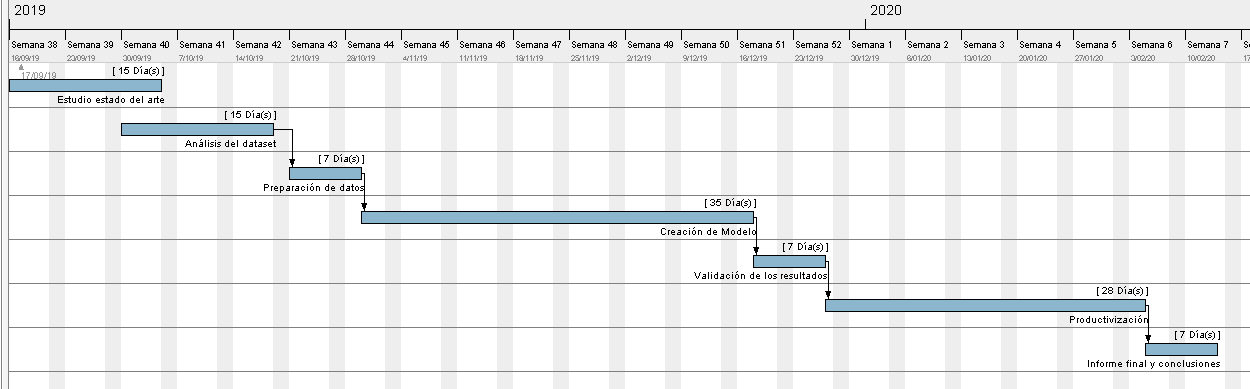
\includegraphics[width=\textwidth]{images/intro/gantt}
	\caption{Diagrama de Gantt}
	\label{fig:gantt}
\end{figure}


\begin{itemize}
	\item \textbf{Estudio estado del arte}: En esta fase se realizará una prospección para conocer el estado del arte en todos los puntos relacionados con el proyecto: Procesamiento del Lenguaje Natural, tecnologías de tratamiento de datos en tiempo real y \textit{Big Data}. 
	
	\item \textbf{Análisis del \textit{dataset}}: El propósito de esta tarea es entender el \textit{dataset}  y estudiar las posibilidades del mismo. 
	
	\item\textbf{ Preparación del \textit{dataset}}: Una vez realizado el estudio del \textit{dataset} es necesario realizar labores de limpieza y transformación de los datos de modo que estos datos sean válidos para nuestro objetivo.
	
	\item \textbf{Creación del modelo}: En esta fase se procederá a la creación de un modelo capaz de obtener los temas de los que habla una determinada llamada. Este modelo será el \textit{core} de nuestro proyecto.
	
	\item \textbf{Validación de los resultados}: Una vez entrenado el modelo será necesario validar los resultados obtenidos para poder evaluar la bondad de nuestro modelo. 
	
	\item\textbf{ Productivización}: El trabajo no acaba con la creación de un buen modelo que nos permita extraer los temas de nuestras llamadas. Este modelo tendrá que ser puesto en producción y permitir al usuario final extraer los temas de las llamadas en tiempo real y darle la opción de crear alarmas basadas en la variación del número de eventos (llamadas) de un determinado tema.
	\item\textbf{ Informe final y conclusiones}: Por último, una vez llevado a a producción nuestro modelo, se realizará un informe final donde, entre otros puntos, se evaluarán los resultados obtenidos y se extraerán conclusiones y pasos futuros.
\end{itemize} 

\begin{figure}[!ht]
	\centering
	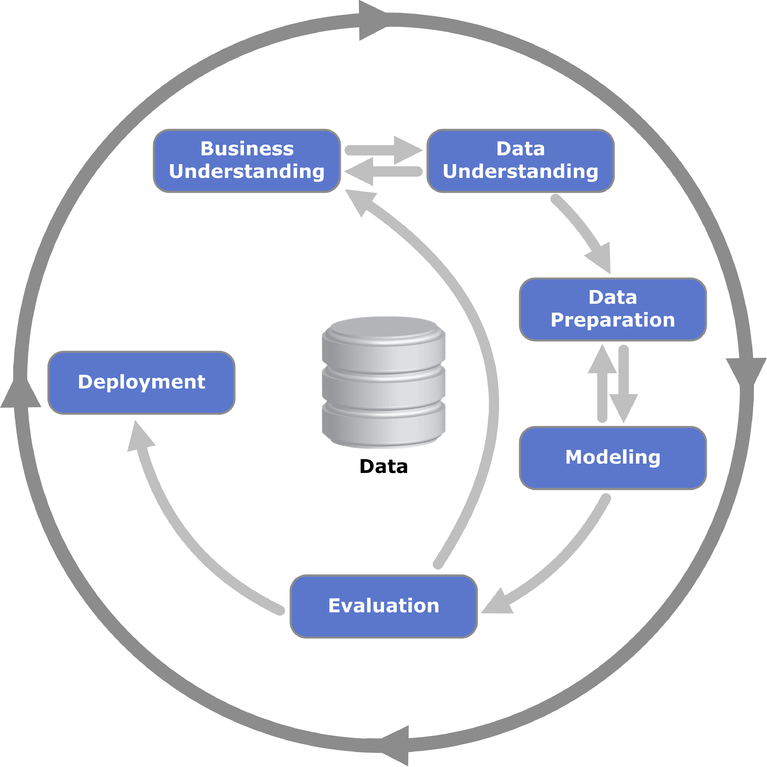
\includegraphics[width=0.63\textwidth]{images/intro/crispdm}
	\caption{Fases del modelo CRISP-DM}
	\label{fig:crispdm}
\end{figure}


Estas fases están basadas en el estándar \textbf{\textit{CRISP-DM}} (\cite{crispdm}), añadiendo una última tarea para nuestro informe final, CRISP-DM nos proporciona una descripción del ciclo de vida de los proyectos de minería de datos de un modo bastante similar al que se aplica en los modelos de ciclo de vida de desarrollo \textit{software}.


 

En la Figura \ref{fig:crispdm} se observa el diseño de este modelo y cómo representa el ciclo de vida de un proyecto de minería de datos. En la imagen podemos ver en primer lugar un círculo exterior que refleja la naturaleza cíclica de los proyectos de minería de datos, además vemos cómo la secuencia de tareas no es rígida, pudiendo saltar hacia adelante o atrás entre tareas. En la gráfica se representan mediante flechas las dependencias más importantes y usuales entre tareas.

En nuestro desarrollo usaremos este modelo, aunque en el diagrama de la Figura \ref{fig:gantt} aparezca una secuencia de tareas más rígida, será usual, por ejemplo, el salto recíproco entre las fases de preparación de los datos y creación del modelo.


\section{Estructura del documento}
\label{section:intro:estructura}
Antes de finalizar el capítulo dedicado a la introducción queremos hacer un breve recorrido por la estructura del documento que presentamos.


El documento presentado  consta de cuatro partes bien diferenciadas: introducción, modelado, explotación y conclusiones. En la figura \ref{fig:esqu} podemos ver un esquema gráfico con la estructura del documento.  A continuación detallaremos las cuatro partes del mismo con los capítulos que las componen: 

\begin{enumerate}[I.]
\item \textbf{Introducción: Objetivos, estado del arte y arquitectura global}.  Esta primera parte pretende servir de introducción al resto del documento presentando la motivación y los objetivos del proyecto, analizando el estado del arte y mostrando finalmente una introducción a la arquitectura global del proyecto. Estará compuesto por los siguientes capítulos:

\begin{enumerate}[1.]
\item Introducción
\item Estado del arte
\item Arquitectura global
\end{enumerate}

\item \textbf{Modelado: datos, modelos y optimizaciones}. Esta segunda parte tratará 

\begin{enumerate}[1.]
\setcounter{enumii}{3}
\item Conjunto de datos
\item Aprendizaje no supervisado
\item Aprendizaje supervisado 
\end{enumerate}


\item \textbf{Explotación: procesamiento, visualización y alarmados}.
\begin{enumerate}[1.]
\setcounter{enumii}{6}
\item Capa de \textit{streaming}.
\item Capa de servicio. 
\item Despliegue en contenedores. 
\end{enumerate}
\item \textbf{Conclusiones: mantenimiento y futuros trabajos}.
\begin{enumerate}[1.]
\setcounter{enumii}{9}
\item DevOps.
\item Conclusiones. 
\end{enumerate}
\end{enumerate}



\chapter{Estado del Arte}
\label{chapter:estadoarte}


El objetivo de este apartado es hacer un recorrido por el estado del arte relacionado con el proyecto, este recorrido lo enfocaremos desde tres puntos de vista diferentes:
\begin{itemize}
	\item \textbf{Procesamiento del Lenguaje Natural}: En la sección \ref{section:arte:pln}  nos centraremos en el procesamiento del lenguaje natural y su evolución a lo largo del tiempo. 
	\item \textbf{\textit{Deep Learning} y aplicación al Procesamiento del Lenguaje Natural}: En la sección \ref{section:arte:deep}  pondremos foco en el \textit{Deep Learning}, sus ventajas y cómo se están aplicando estos métodos al procesamiento del lenguaje natural. 
	\item \textbf{\textit{Big Data} y \textit{Fast Data}}: Por último, en la sección \ref{section:arte:big}, haremos un repaso a la evolución del \textit{Big Data} y cómo la tendencia actual es realizar el procesamiento en tiempo real mediante \textit{Fast Data}.
\end{itemize}

Por último, una vez analizados los diferentes puntos de vista, en la sección \ref{section:arte:ant} enumeraremos trabajos anteriores relacionados con nuestro proyecto. Estos trabajos nos serán de utilidad para justificar la realización de nuestro proyecto y su viabilidad. 

\section{Procesamiento de lenguaje natural}
\label{section:arte:pln}

\subsection{Historia}

Para hablar de los orígenes del Procesamiento del Lenguaje Natural (a partir de ahora se usarán indistintamente las siglas PLN) tal y como lo conocemos, tendríamos que remontarnos a los años 50, concretamente al artículo ``\textit{Computing Machinery and Intelligence}'' escrito por Alan Turing \cite{turing_1950}. En este artículo aparece el PLN dentro del campo de la inteligencia artificial y se presenta por primera vez el conocido ``Test de Turing`''. Este test convirtió la pregunta abstracta de ``¿Son capaces de pensar las máquinas?'' en un juego llamado: ``\textit{The Imitation Game}''. El juego propuesto inicialmente, de forma muy resumida, consiste en ver si una persona (interrogador) interrogando a dos personas (un hombre y una mujer), era capaz de descubrir el sexo de cada una; la modificación del mismo sustituye las dos personas de distinto sexo por una persona y una máquina y el interrogador debe ser capaz de descubrir si las preguntas están siendo respondidas por un humano o una máquina. En el caso de que no sepa discernir, la computadora gana la partida. Podemos encontrar más información al respecto en el libro \cite{turing}.



A partir de los avances de Turing y hasta los años 80 el crecimiento en el campo del PLN se produjo principalmente con la creación de complejos sistemas basados en reglas escritas a mano. Fue en esta década cuando empezamos a vivir la incorporación de algoritmos de \textit{Machine Learning} enfocados al procesamiento del lenguaje natural. Este hecho se vio motivado principalmente por el increíble avance en la capacidad de cómputo, ya predicho por la ley de Moore, y por la aplicación de teorías ya existentes como los trabajos de Chomsky. 


Desde el comienzo de la aplicación de modelos de \textit{Machine Learning}, y de nuevo motivados por el crecimiento de la capacidad computacional de los sistemas actuales, se ha pasado de utilizar árboles de decisión, que creaban de manera automática reglas similares a las que se venían creando manualmente, a los modelos de \textit{deep learning} que están en auge en la última década. 

\subsection{Aplicaciones}

En el apartado anterior hicimos referencia a ``\textit{The Imitation Game}'' como inicio de lo que hoy conocemos como procesamiento del lenguaje natural, sin embargo, las aplicaciones en este campo han crecido de forma vertiginosa en estos 70 años, principalmente en las últimas décadas. Hoy en día, si tuviéramos que contestar a la pregunta: ``¿son capaces de pensar las máquinas?'', implicaría algo más que superar el test de Turing. Mirando a nuestro alrededor nos encontraríamos con asistentes de voz como Alexa o Siri que, no solo contestan a nuestras preguntas, si no que realizan un trabajo de pasar nuestra voz a texto (\textit{Speech to Text}) y de nuevo el texto resultante a voz (\textit{Text to Speech}). Nos encontraríamos también con sistemas capaces de realizar traducciones simultáneas, otros capaces de autocompletar textos, de identificar preguntas y respuestas, de clasificar textos de acuerdo a temas o autores, incluso de analizar sentimientos positivos o negativos teniendo como entrada un texto u opinión.


Según \cite{goldberg_2017} todos estos problemas tan diversos podríamos clasificarlos según en el punto del análisis que nos centremos: 

\begin{itemize}
	\item \textbf{Análisis de palabras}: En este tipo de problemas se pone foco en las palabras, como pueden ser ``perro'', ``hablar'', ``piedra'' y necesitamos decir algo sobre ellas. Por ejemplo: ``¿estamos hablando de un ser vivo?'', ``¿a qué lenguaje pertenece?'', ``¿cuáles son sus sinónimos o antónimos?''. Actualmente este tipo de problemas son menos frecuentes, ya que normalmente no pretendemos analizar palabras aisladas sino que es preferible basarse en un contexto. 
	
	\item \textbf{Análisis de textos}:  En este tipo de problemas no trabajamos solo con palabras aisladas, sino que disponemos de una pieza de texto que puede ser una frase, un párrafo o un documento completo y tenemos que decir algo sobre él. Por ejemplo: ``¿se trata de spam?'', ``¿qué tipo de texto es?'', ``¿el tono es positivo o negativo?'', ``¿quién es su autor?''. Este tipo de problemas son muy comunes y nos vamos a referir a ellos como \textbf{problemas de clasificación de documentos}.   
	
	\item \textbf{Análisis de textos pareados}: En esta clase de análisis disponemos de  dos textos (también podrían ser palabras aisladas) y tenemos que decir algo sobre ellos. Por ejemplo, ``¿los textos son del mismo autor?'', ``¿son pregunta y respuesta?'', ``¿son sinónimos?'' (para el caso de palabras aisladas).
	
	\item \textbf{Análisis de palabras en contexto}: En estos casos de uso, a diferencia del primer análisis que trataba unicamente con  palabras aisladas, tenemos que clasificar una palabra en particular en función del contexto en el que se encuentra. 
	
	\item \textbf{Análisis de relación entre palabras}: Este último tipo de análisis tiene como objetivo deducir la relación entre dos palabras existentes en un documento. 
	
\end{itemize}

Dependiendo del problema que queramos abordar usaremos un tipo de características del lenguaje u otro, por ejemplo, es usual que si estamos analizando palabras aisladas nos centremos en las letras de una palabra, sus prefijos o sufijos, su longitud, la información léxica extraída de diccionarios como \textit{WordNet} \cite{wordnet}, etc. En cambio, si estamos trabajando con texto, lo normal es que nos fijemos en otros conceptos estadísticos como el histograma de las palabras dentro del texto, ratio de palabras cortas vs largas, número de veces que aparece una palabra en un texto comparado con el resto de textos, etc.

El proyecto que se presenta en este documento está centrado en el análisis de textos, concretamente en extraer los temas de un documento (o llamada). Este tipo de problemas se conoce como modelización de \textit{topics}. 

En el siguiente punto de este apartado nos centraremos en algunos modelos y avances en este área que puedan servirnos de apoyo para nuestro proyecto. 


\subsection{Modelización de temas}
\label{section:arte:lda}
La modelización de topics hace referencia a un grupo de algoritmos de \textit{Machine Learning} que infieren la estructura latente existente en un grupo de documentos. 


Aunque la mayoría de los algoritmos de modelización son no supervisados, al igual que los algoritmos tradicionales de \textit{clustering}, existen también algunas variantes supervisadas que necesitan disponer de documentos etiquetados. 


\begin{figure}[!ht]
	\centering
	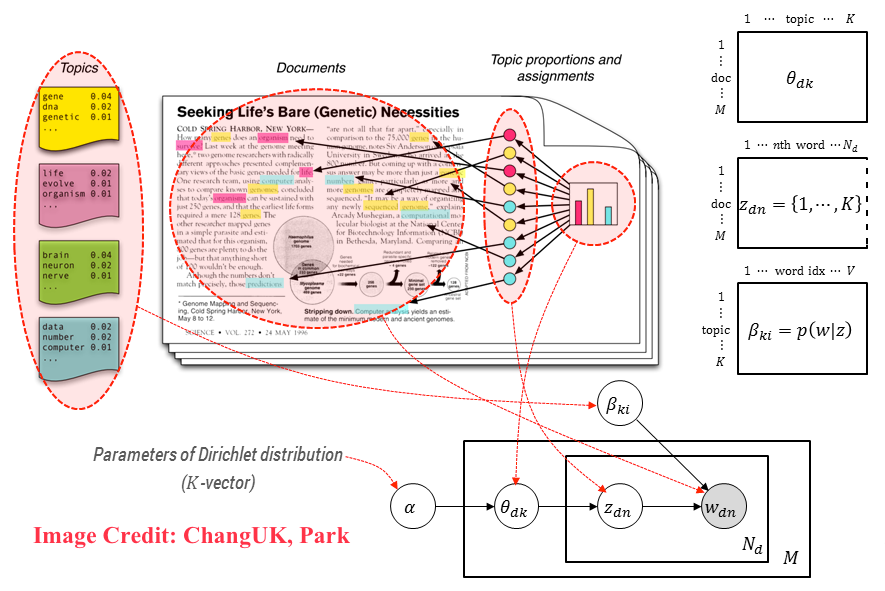
\includegraphics[width=0.68\textwidth]{images/arte/lda}
	\caption{Representación gráfica de LDA. Fuente \cite{ldafig}}
	\label{fig:lda}
\end{figure}


Quizás el algoritmo más conocido para la modelización de topics sea el \textit{Latent Dirichlet Allocation} (normalmente conocido por su acrónimo, LDA). LDA fué presentado en 2003 en el artículo \cite{Blei_LDA} y podemos ver una representación gŕafica del mismo en la figura \ref{fig:lda}. Este algoritmo no supervisado asume que cada documento es una distribución probabilística de \textit{topics} y cada \textit{topic}, a su vez, es una distribución de palabras del documento. LDA usa una aproximación llamada ``\textit{bag of words}'', en la que cada documento es tratado como un vector con el conteo de las palabras que aparecen en el mismo. La principal característica de LDA es que la colección de documentos comparten los mismos topics, pero cada documento contiene esos topics en una proporción diferente. 


A partir de LDA surgieron numerosas variantes que repasaremos de forma breve, por ejemplo, en el mismo año de la creación de LDA y también presentado por los mismos autores en \cite{Blei_HTM}, surgió una \textbf{variante jerárquica} que permitía representar los \textit{topics} jerárquicamente. En 2006 en \cite{Blei_DTM} se desarrolla un modelo LDA dinámico denominado DTM (\textit{Dinamic Topic Model}), en el que se introduce la variable temporal y los \textit{topics} pueden ir cambiando a lo largo del tiempo. En el artículo \cite{Blei_CTM} nos encontramos con otra variante de LDA llamada CTM (\textit{Correlated topic model}) que nos permite encontrar correlaciones entre \textit{topics}, ya que algunos temas es probable que sean más similares entre sí. Por último, nos encontramos con una variante de LDA denominada ATM (\textit{Author-Topic Model}) propuesta  por	Michal Rosen-Zvi en su artículo \cite{Rosen-Zvi_AMA_2010}  y desarrollada por el mismo en 2010, en la que los documentos son una distribución probabilística tanto de autores como de \textit{topics}.    


Podemos encontrar un resumen más completo del estado del arte en cuanto a la modelización de \textit{topics} en el artículo \cite{Mahmood2013LiteratureSO}. 

\section{Deep Learning  y aplicación al PLN}
\label{section:arte:deep}

El objetivo de esta sesión es entender el concepto de \textit{Deep Learning} y analizar el estado del arte del \textit{Deep Learning} aplicado al Procesamiento del Lenguaje Natural. Para poder entender el \textit{Deep Learning} es conveniente entender los modelos de aprendizaje supervisados y saber qué provoca su aparición y popularidad de los últimos años. Posteriormente nos centraremos en los fundamentos del \textit{Deep Learning} y cómo es utilizado en la representación de palabras. Por último, comentaremos algunas arquitecturas especializadas y su aplicación en el ámbito del Procesamiento del Lenguaje Natural.


\subsection{Aprendizaje supervisado}
El aprendizaje supervisado consiste en aprender una función a través de un conjunto de datos llamados de entrenamiento, mediante la cual podamos obtener una salida a partir de una determinada entrada. Se espera que esta función, una vez realizado el entrenamiento, sea capaz de producir una salida correcta incluso para datos nunca vistos. Es muy habitual el uso de estos tipos de algoritmos para casos de clasificación y/o predicción. 

Buscar entre todas las posibles infinitas funciones para encontrar la que mejor se adapte a nuestro conjunto de datos es un trabajo inviable, es por ello que normalmente se realiza la búsqueda entre un conjunto de funciones limitadas. En un primer lugar, y hasta hace aproximadamente una década, los modelos más populares de aprendizaje supervisado fueron los modelos lineales, provenientes del mundo de la estadística, estos modelos son fáciles de entrenar, fáciles de interpretar y muy efectivos en la práctica. 

A partir de entonces, y motivado en parte por el aumento en las capacidades de cómputo, surgen otros modelos como las máquinas de vectores de soportes (\textit{Support Vector Machines}, SVMs) o las redes neuronales, en las que nos centraremos en el siguiente apartado.


\subsection{Deep Learning}
Dentro del \textit{Machine Learning} y usualmente relacionado con el aprendizaje supervisado, nos encontramos con un sub-campo denominado \textbf{Deep Learning} que utiliza las redes neuronales para la creación de modelos. 

Como su nombre indica las redes neuronales consisten en unidades de cómputo llamadas neuronas que están interconectadas entre sí. Una neurona es una unidad de cómputo que posee múltiples  entradas y una  salida, esta neurona multiplica cada entrada por un peso para posteriormente realizar una suma y, por último, aplicar una función de salida no lineal. Si los pesos se establecen correctamente y tenemos un número suficiente de neuronas, una red neuronal puede aproximar a un conjunto muy amplio de funciones matemáticas. 

En las redes neuronales, las neuronas suelen organizarse por capas que se encuentran conectadas entre sí. Mientras más capas tengamos, más características podremos extraer de nuestros datos de entrada y podremos aproximar un mayor número de funciones (sin perder de vista el sobrentrenamiento). 


El primero y más simple de los tipos de redes neuronales es el denominado \textit{Feed Forward Neural Network} (\textbf{FFNN}), este tipo de redes recibe este nombre porque no existen ciclos entre sus neuronas y las conexiones se realizan siempre desde las capas anteriores a las capas posteriores. 


Una de las arquitectura más comunes de FFNN es el preceptrón multicapa (en inglés multilayer perceptron o \textbf{MLP}). Esta arquitectura contiene tres o más capas de neuronas totalmente conectadas, es decir, la salida de una neurona de una capa se encuentra conectada a la entrada de todas las neuronas de la siguiente capa. Las capas de una arquitectura MLP son:

\begin{itemize}
	\item \textbf{Capa de entrada}: Se trata de la capa en la que introduciremos los datos en la red. Esta capa carece de procesamiento.
	\item \textbf{Capas ocultas}: Son las capas intermedias, cuyo número puede variar, tienen como entrada la salida de las neuronas de la capa anterior y su salida alimenta a las neuronas de la capa posterior.  
	\item \textbf{Capa de salida}: Los valores de salida de las neuronas de esta capa se corresponden con la salida de la red.
\end{itemize}
 
\begin{figure}[!ht]
	\centering
	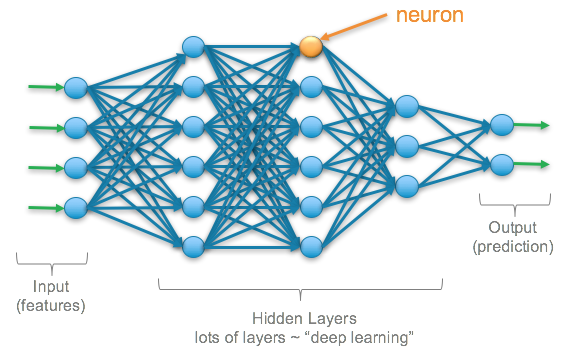
\includegraphics[width=0.68\textwidth]{images/arte/mlp}
	\caption{Ejemplo de arquitectura MLP. Fuente \cite{mlp}}
	\label{fig:mlp}
\end{figure}



Hablamos que una red es profunda cuando contiene un gran número de capas, por ello el término de \textit{Deep Learning}. En la Figura \ref{fig:mlp} observamos un ejemplo de arquitectura MLP y como la denominamos \textit{Deep Learning} al crecer el número de capas ocultas.


\subsection{Representación de palabras en PLN}% Podemos llamarle embedding o representación de palabras

Es usual, en el ámbito del reconocimiento de imágenes, utilizar información acerca de la dimensionalidad de las mismas. Este tipo de información nos permite extraer características  teniendo en cuenta los píxeles vecinos. Tradicionalmente, en el ámbito del Procesamiento del Lenguaje Natural, esto no se ha llevado a cabo debido a que cada palabra (o n-grama) se trataba como una entidad aislada utilizando una codificación de las palabras denominada \textbf{one-hot encoding}. 

En cambio, existe otro método de representar las palabras en el lenguaje natural que sí es capaz de captar la ``dimensionalidad'' de una forma similar a como lo realizamos en las imágenes. Este modo, conocido como \textit{\textbf{word embedding}}, deja de tratar la palabra como un ente aislado y  es capaz de captar el significado de la misma, esta representación se denomina distribuida y consiste en convertir las palabras en vectores en los que cada dimensión capte características diferentes de las palabras. Este tipo de representaciones dará lugar a vectores similares para palabras semánticamente parecidas. 


\begin{figure}[!ht]
	\centering
	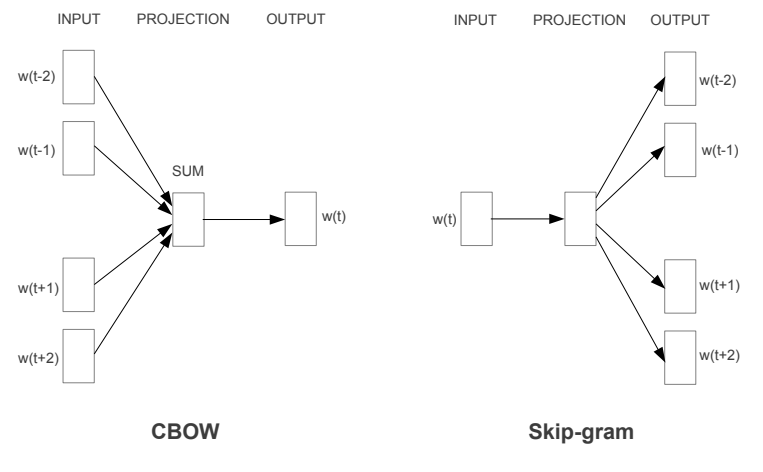
\includegraphics[width=0.7\textwidth]{images/arte/word2vec}
	\caption{Arquitecturas CBOW y Skip-gram. Fuente \cite{word2vec}}
	\label{fig:wor2vec}
\end{figure}

Una de las soluciones más populares que nos permiten convertir una palabra a un vector (\textit{word2vec}) que contenga información de la palabra en función del contexto se detallan en el artículo \cite{word2vec} . Aquí se presentaron dos modelos llamados \textbf{Skip-Gram} y \textbf{CBOW} cuya arquitectura podemos ver en la Figura \ref{fig:wor2vec}. Estos modelos utilizan redes neuronales para predecir una palabra en función de su contexto o el contexto en función de una palabra, el vector que se utiliza para representar la palabra es el vector de pesos de la capa oculta. 



\subsection{Arquitecturas especializadas}

Después de introducir las redes neuronales y el modo en el que podemos representar las palabras, frases o documentos para ser usados como entrada en nuestro modelo; vamos a centrarnos en comentar dos tipos de redes neuronales que se usan de manera tradicional en tareas de Procesamiento de Lenguaje Natural. 

Los dos tipos de redes neuronales que comentaremos son las redes neuronales convolucionales y las redes neuronales recurrentes. Haremos una introducción a cada una de ellas, comentaremos sus aplicaciones al PLN y sus ventajas e inconvenientes con respecto a otro tipo de métodos. 


\subsubsection{Redes neuronales convolucionales}
\label{section:arte:arqu:cnn}

Las redes neuronales convolucionales (llamadas usualmente CNN, por su nombre en inglés \textit{\textbf{C}onvolutional \textbf{N}eural \textbf{N}etworks}) son un tipo de redes neuronales que deben su nombre a la operación matemática de convolución que realizan. Esta operación consiste en aplicar a una matriz de entrada multidimensional, un filtro o kernel también multidimensional y obtener una salida, también denominada mapa de características. En la Figura \ref{fig:cnn1} podemos ver una representación gráfica de esta operación para un ejemplo de 2 dimensiones. 

\begin{figure}[!ht]
	\centering
	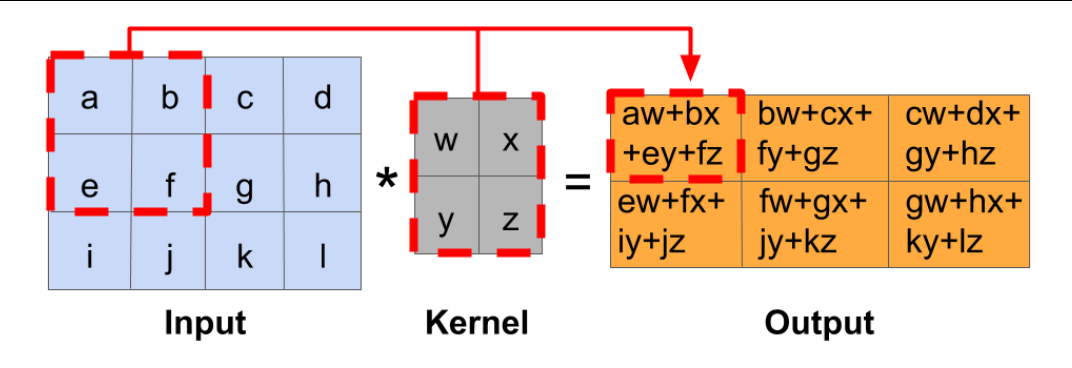
\includegraphics[width=0.7\textwidth]{images/arte/cnn1}
	\caption{Ejemplo de una convolución de dos dimensiones. Fuente \cite{temariodeeplearning}}
	\label{fig:cnn1}
\end{figure}

Es usual en las redes convolucionales  utilizar diferentes kernels sobre una misma entrada, obteniendo diferentes salidas que permitan reconocer distintos patrones. Los pesos del kernel junto con el sesgo, son los parámetros que serán necesarios calcular en el entrenamiento y en el caso de las redes convolucionales, se denominan mapas de características.

Aunque la convolución simple que comentamos es la operación básica en las redes convolucionales, es usual añadirle algunas variantes (o configurarla con algunos parámetros) que nos permitan variar la dimensión de salida una vez hemos aplicado la convolución; algunas de estas variaciones más comunes son el \textbf{\textit{zero padding}} y la \textbf{convolución por pasos}.

\begin{figure}[!ht]
	\centering
	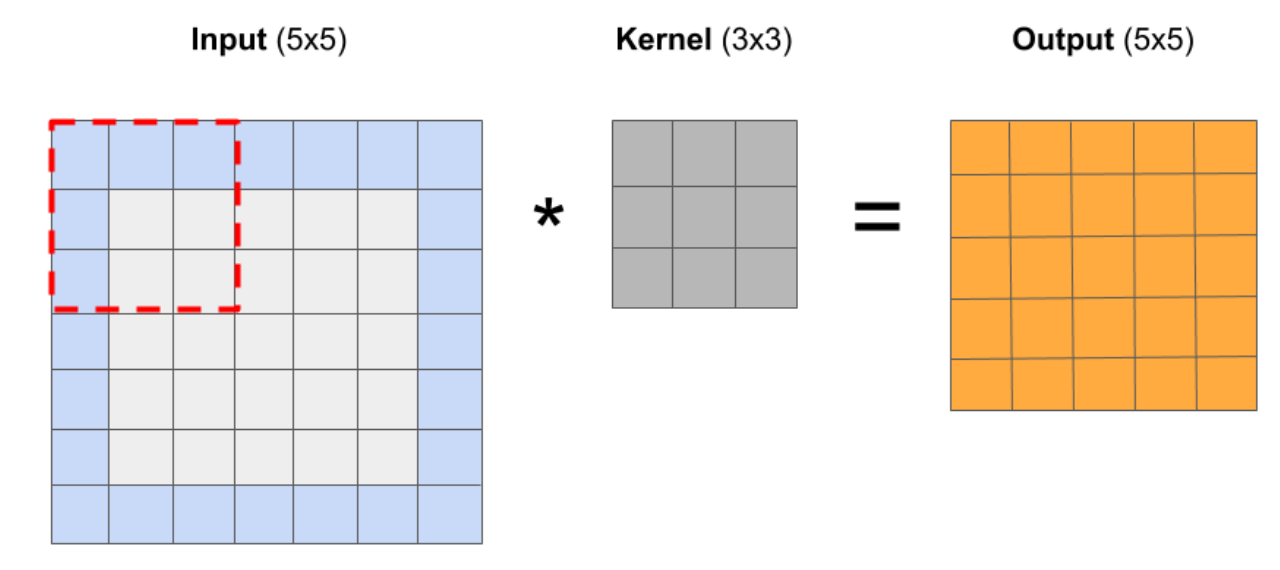
\includegraphics[width=0.7\textwidth]{images/arte/padding}
	\caption{Ejemplo de aplicación de \textit{zero padding} para mantener la dimensionalidad. Fuente \cite{temariodeeplearning}}
	\label{fig:padding}
\end{figure}

Como observamos en la Figura \ref{fig:cnn1}, al aplicar el kernel a los datos de  entrada estamos reduciendo la dimensionalidad de la salida. A menudo es posible que esto no nos interese y queramos mantener la dimensionalidad en la salida; para ello recurrimos a un método denominado \textit{zero padding} que consiste en añadir '0s' en los bordes de nuestra entrada con el objetivo de preservar la dimensionalidad en la salida. En la Figura \ref{fig:padding} podemos ver un ejemplo de aplicación de \textit{zero padding}.




Por otro lado, es también posible que queramos reducir aún más la dimensión de salida, principalmente por un tema de eficiencia y reducción de los tiempos de ejecución, a costa de perder información de algunas características en la salida. Para ello podemos utilizar la convolución por pasos (o \textit{strided} por su nombre en inglés). Este método consiste en aplicar el kernel realizando saltos en lugar de hacerlo sobre celdas consecutivas,  tal y como podemos ver en la Figura \ref{fig:strided}.

\begin{figure}[!ht]
	\centering
	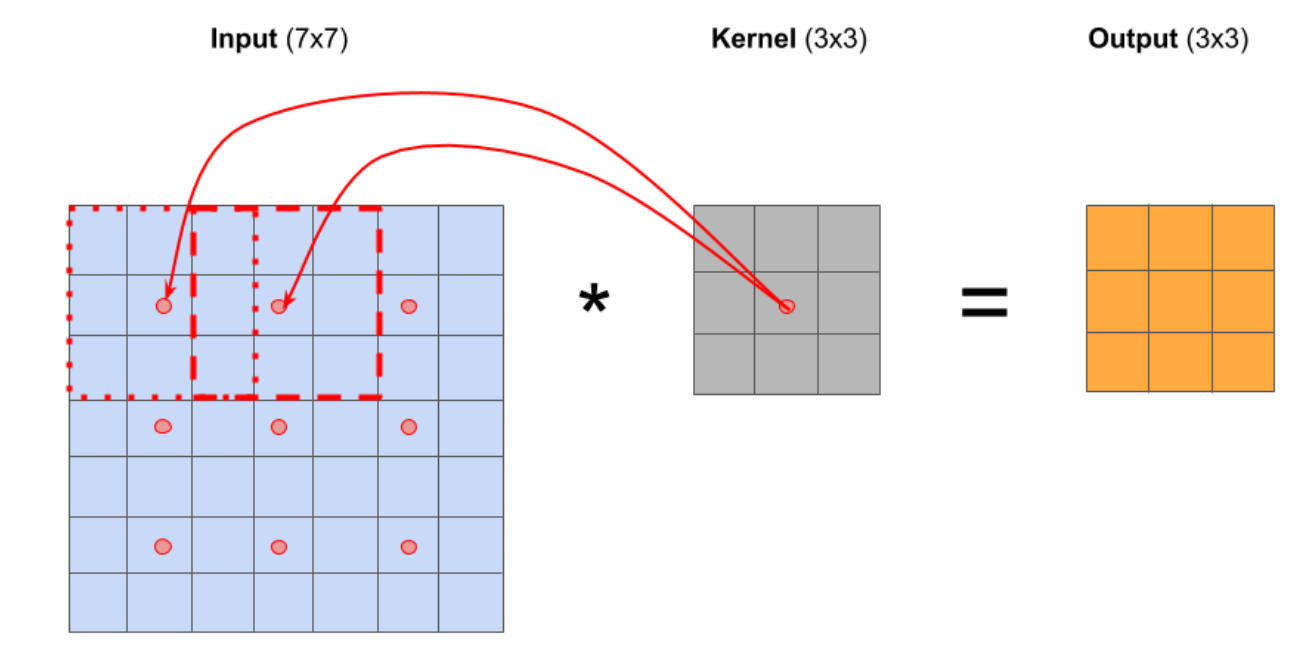
\includegraphics[width=0.7\textwidth]{images/arte/strided}
	\caption{Ejemplo de aplicación de convolución por pasos para reducir la dimensionalidad. Fuente \cite{temariodeeplearning}}
	\label{fig:strided}
\end{figure}



El proceso explicado anteriormente correspondería con una capa convolucional, que son el corazón de las redes neuronales convolucionales, sin embargo, en una red neuronal convolucional estas capas coexisten con otro tipo de capas que nos ayudaran a mejorar nuestros modelos. Las más usuales son:

\begin{itemize}
	\item Capa de agrupamiento (\textit{polling} en inglés): El objetivo de esta capa es agrupar un conjunto de salidas para obtener un único valor. Al conjunto de valores de entrada (seleccionado de nuevo con un filtro) se le aplica una función para obtener un único valor. Aunque se pueden utilizar diferentes funciones, como puede ser la media, lo más usual es aplicar la función de máximo (\textit{max-polling}). Es habitual, intuir que usando esta función nos estamos quedando con las características más relevantes de cada cuadrante (del tamaño del filtro) de la entrada. En la Figura \ref{fig:pooling} podemos ver un ejemplo de agrupamiento utilizando la función de máximo. 
	\item Capa totalmente conectada: Hemos visto ejemplos de capas totalmente conectadas al introducir las redes neuronales, esta capas usualmente se usan al final de nuestra red para tareas de clasificación, teniendo la última capa un número de neuronas igual al número de clases que pretendemos clasificar. 
	\item Capa RELU: Si observamos la descripción de la operación de convolución nos damos cuenta de que se trata de una operación totalmente lineal, es por ello que después de cada capa de convolución es usual agregar una capa no lineal (también llamada capa de activación). Aunque se pueden utilizar otras funciones como la tangente o la función sigmoide, lo más usual es utilizar la función RELU.
	
	\item Capa de Dropout: Esta capa tiene como funcionalidad prevenir el sobreentrenamiento en las redes neuronales, desactivando un número aleatorio de entradas de la capa, forzando a la red a ser redundante y permitiendo dar una clasificación correcta sin tener todas las entradas activas. 
	
\end{itemize}

\begin{figure}[!ht]
	\centering
	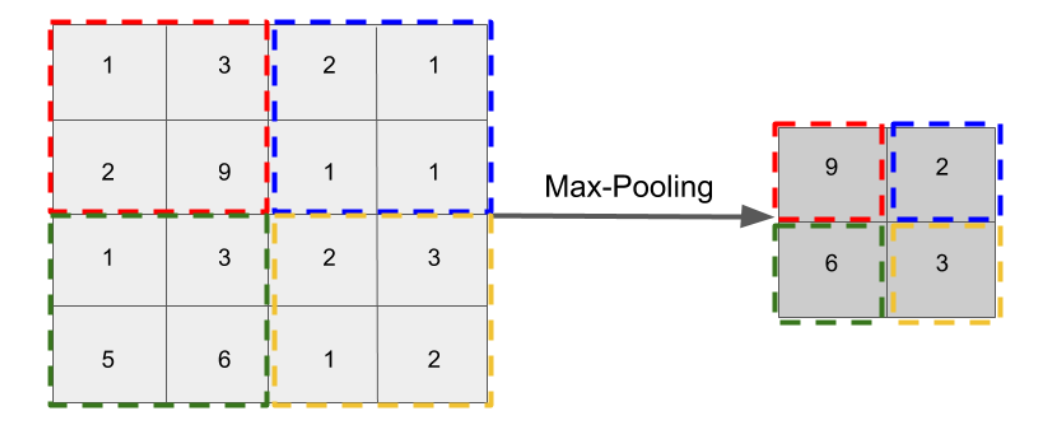
\includegraphics[width=0.7\textwidth]{images/arte/pooling}
	\caption{Ejemplo de aplicación de \textit{max-pooling}. Fuente \cite{temariodeeplearning}}
	\label{fig:pooling}
\end{figure}


Tras esta visión general sobre las redes neuronales generales, podemos enumerar las ventajas que conllevan: 

\begin{itemize}
	\item Por un lado, aunque no hemos entrado en detalles sobre el proceso de entrenamiento de las redes convolucionales, se puede intuir que el aplicar un mismo kernel sobre toda la entrada provoca que el número de parámetros a aprender (los valores del kernel) con respecto a una red totalmente conectada será mucho menor. Esto provoca una \textbf{reducción del tiempo de entrenamiento necesario}. 
	\item Por otro lado, el hecho de compartir el kernel provoca que podamos \textbf{capturar una misma característica en la entrada a pesar de su traslación}. Por ejemplo, si estamos detectando un objeto en una imagen un modelo convolucional podrá detectar ese objeto a pesar de su movimiento por la imagen. 
\end{itemize}


\begin{figure}[!ht]
	\centering
	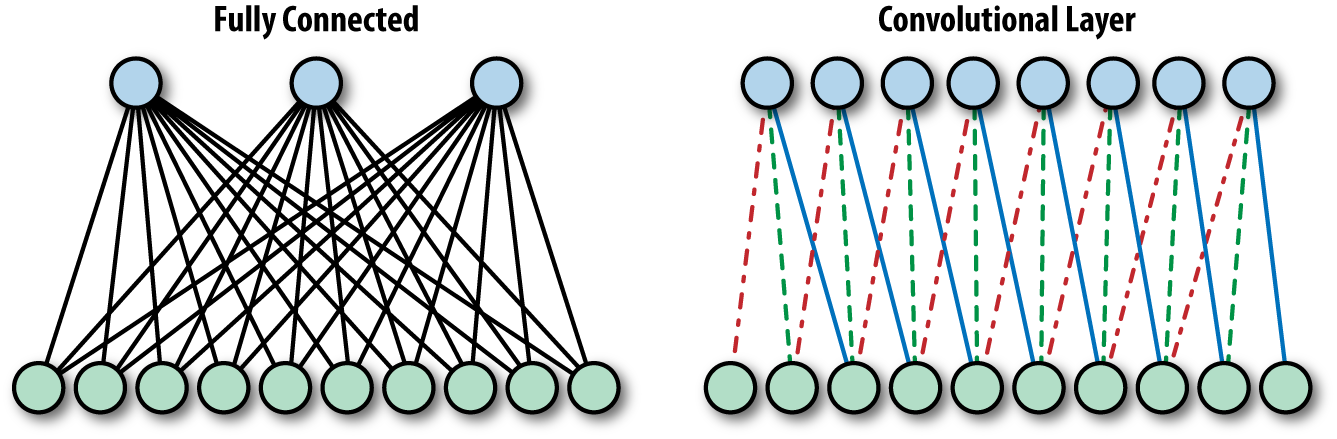
\includegraphics[width=0.7\textwidth]{images/arte/traditionalvscnn}
	\caption{Comparación capa tradicional totalmente conectada con capa convolucional. Fuente \cite{hope_lieder_resheff_2017}}
	\label{fig:tradvscnn}
\end{figure}



Sin embargo, las redes neuronales convolucionales deben usarse en datos que contengan coherencia local ya que esa es su fortaleza. \textbf{En datos sin coherencia local las redes neuronales convolucionales no lograrían obtener un buen rendimiento} como las redes neuronales tradicionales vistas anteriormente. Si observamos la Figura \ref{fig:tradvscnn} podemos ver la diferencia entre las capas de ambos tipos de redes y cómo la capa convolucional se centra más en las estructuras locales.




Encontramos una explicación más profunda sobre las redes convolucionales y su uso general en \cite{temariodeeplearning}. Aunque, como podemos imaginar, el uso más extendido de este tipo de redes es para el tratamiento de imágenes, nosotros nos centraremos en tener una breve visión de su aplicación al Procesamiento del Lenguaje Natural, que también puede ampliarse en \cite{goldberg_2017}.



Al aplicar las redes tradicionales al PLN, solemos ignorar el orden en el que las palabras aparecen en las frases, o las frases en el documento, siguiendo una aproximación CBOW;  esto suele ser problemático a la hora de realizar, por ejemplo, un análisis de sentimientos ya que no es lo mismo encontrar la palabra ``malo'' aislada que el bigrama ``no malo''. Aunque el uso de bi-gramas y N-gramas de mayor orden puede mejorar esta situación el coste puede volverse inasumible. 

Es en este ámbito dónde las redes neuronales convolucionales pueden ser de gran ayuda, ya que gracias a la capacidad comentada para detectar estructuras locales serían capaces de identificar estos N-gramas de forma automática para ser usados posteriormente en tareas predictivas. 




\subsubsection{Redes neuronales recurrentes}
\label{section:arte:arqu:rnn}

Otro de los modelos usualmente usados en tareas de Procesamiento del Lenguaje Natural son las redes neuronales recurrentes, (llamadas usualmente RNN, por su nombre en inglés \textit{\textbf{R}ecurrent \textbf{N}eural \textbf{N}etworks}). Hasta ahora todos los modelos de redes neuronales que hemos citado funcionaban siempre en una dirección, las neuronas de una capa anterior producían una salida que era la encargada de activar las neuronas de la capa posterior. En las redes recurrentes veremos que las salidas de una neurona en una capa posterior pueden tener una conexión con una neurona de una capa anterior. Esto crea una especie de \textbf{memoria} que nos permite modificar la respuesta de la red en función de los datos que se hayan procesado anteriormente (incluso reaccionar con datos que lleguen posteriormente).

\begin{figure}[!ht]
	\centering
	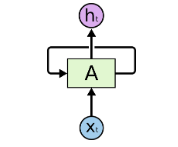
\includegraphics[width=0.32\textwidth]{images/arte/rnn}
	\caption{Ejemplo RNN. Fuente \cite{colahblog}}
	\label{fig:rnn}
\end{figure}

Las conexiones en una red neuronal recurrente pueden tener muchas variaciones por lo que es usual hablar del concepto de \textbf{celda}. Una celda suele tener como entrada los valores de la secuencia y el estado de la red neuronal en el paso anterior; y como salida la respuesta de la red neuronal a dicha entrada y el estado de la red neuronal en el paso actual. 



En la Figura \ref{fig:rnn} observamos un ejemplo de red neuronal recurrente en el que tenemos como entrada el valor de la secuencia $x_{t}$ y el estado de la red en el paso anterior (conexión en bucle). Producimos una respuesta $h_{t}$ y un estado (conexión en bucle). Sin embargo, posiblemente esta representación sea algo más confusa para comprender su funcionamiento que si procedemos a ``desenrollar'' la red neuronal haciéndola más similar a los modelos vistos hasta ahora. En la Figura \ref{fig:rnn2} podemos ver el resultado de ``desenrollar'' la red; hay que tener en cuenta con esta representación que los parámetros usados por cada celda son exactamente los mismos.

\begin{figure}[!ht]
	\centering
	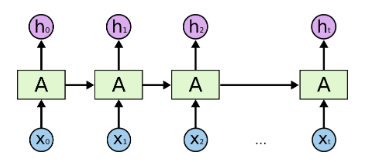
\includegraphics[width=0.65\textwidth]{images/arte/rnn2}
	\caption{Ejemplo RNN ``desenrollada''. Fuente \cite{colahblog}}
	\label{fig:rnn2}
\end{figure}



Aunque no entraremos en detalles sobre el entrenamiento de redes neuronales, es importante saber que existen dos problemas diferentes provocados ambos por usar los mismos parámetros en todas las celdas que provocan la inestabilidad durante el proceso de entrenamiento. Estos problemas son la \textbf{desaparición del gradiente}, que ocurre al multiplicar el gradiente consigo mismo múltiples veces cuando este es menor que 1, y la \textbf{explosión del gradiente}, que ocurre por el mismo motivo cuando este es mayor que 1. 

Para mitigar estos problemas es importante el diseño de las celdas, a continuación veremos de manera resumida los dos tipos de celdas más usados en las redes neuronales recurrentes. Las celdas que comentaremos están compuestas por diferentes mecanismos internos, denominados puertas, que gestionan el flujo de información a lo largo de la misma. 


El primer tipo de celdas  son las celdas \textit{Long Short Term Memory} (\textbf{LSTM}). Este tipo de celdas se comportan bien en situaciones que queremos encontrar patrones entre registros que se encuentran separados en la secuencia, esto es algo muy usual, por ejemplo, en el caso de PLN cuando en una misma frase una palabra hace referencia a otra que apareció a una distancia de varias palabras. 
	
Para conseguir este objetivo, parece evidente que es importante controlar la memoria en cada una de las celdas. Una celda LSTM realiza esta tarea con las siguientes puertas: 
	\begin{itemize}
		\item Puerta de entrada: Controla que información se añade a la memoria de la red. 
		\item Puerta de olvido: Controla, a partir de la memoria del paso anterior y de la entrada, qué información debe conservarse en la memoria. 
		\item Puerta de salida:  Es la encargada de calcular la salida de la red, $h_{t}$, en el paso actual. 
	\end{itemize}

\begin{figure}[!ht]
	\centering
	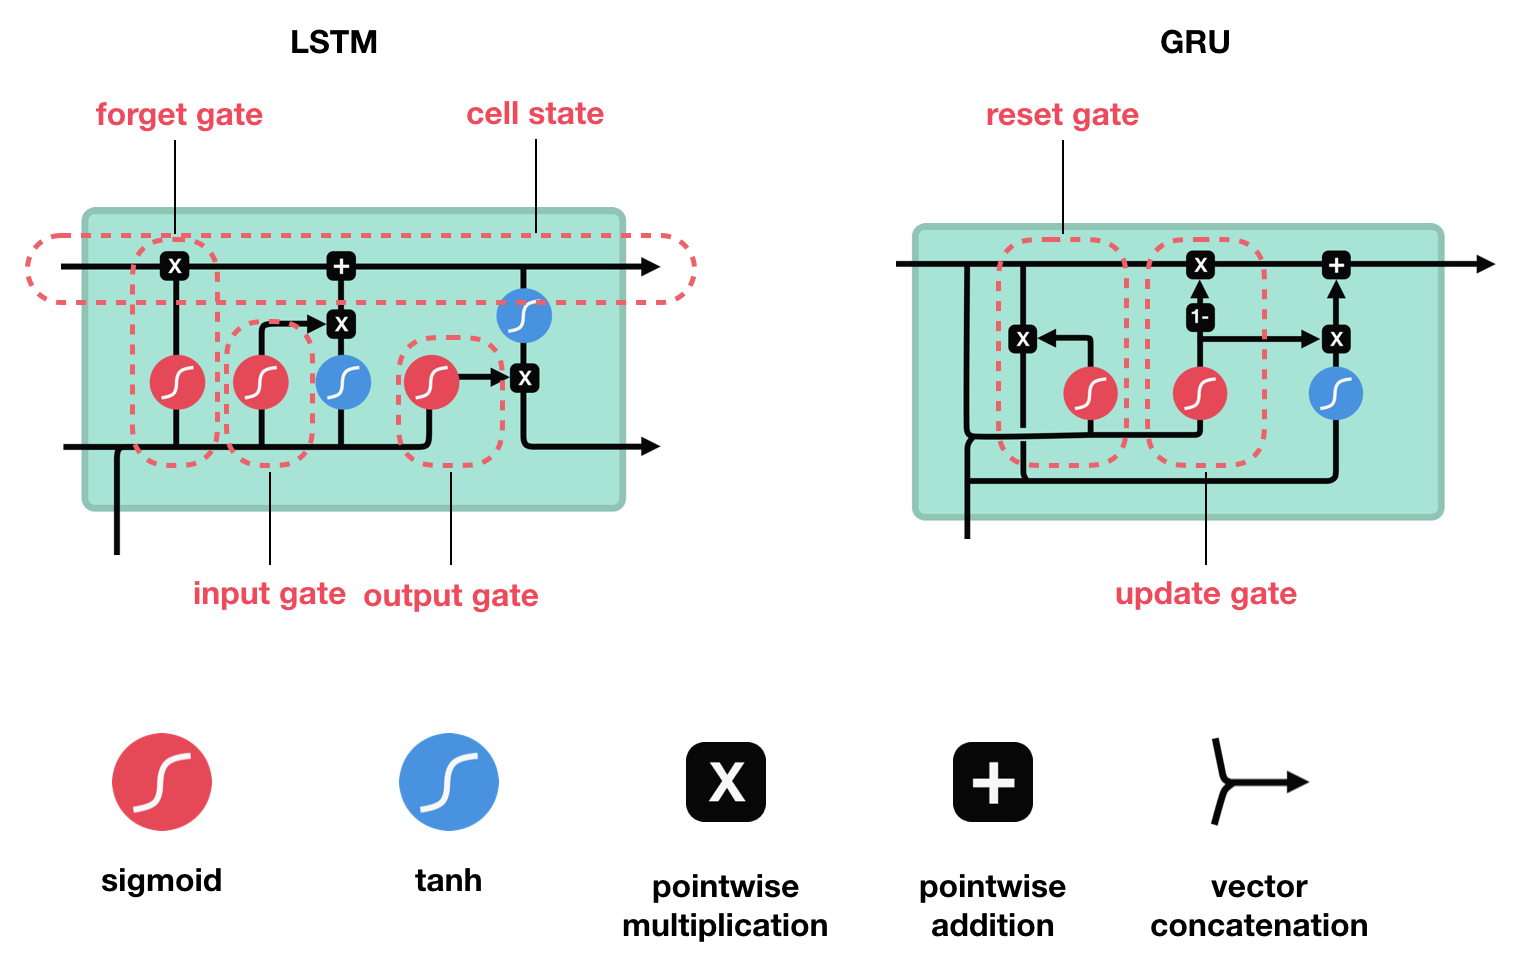
\includegraphics[width=0.84\textwidth]{images/arte/lstmvsgru}
	\caption{Arquitectura celdas LSTM y GRU. Fuente \cite{lstmgru}}
	\label{fig:lstmvsgru}
\end{figure}



Debido al éxito de las celdas LSTM, y al constante esfuerzo de optimización de las mismas, han surgido diferentes variantes. La más conocida de todas son las \textit{Gated Recurrent Unit} (\textbf{GRU}) introducidas en 2014. La celda GRU es una simplificación de la celda LSTM y produce unos rendimientos bastante similares con un menor coste. De manera muy resumida una celda GRU se compone de: 
\begin{itemize}
	\item Puerta de reset: Permite seleccionar que información de la memoria va a ser utilizada en un paso concreto. 
	\item Puerta de actualización: Realiza la función de las puertas de olvido y de entrada que hemos visto en las celdas LSTM.
\end{itemize}

Aunque no hemos entrado en el detalle del funcionamiento de cada una de las puertas, en la Figura \ref{fig:lstmvsgru} podemos ver la arquitectura completa de ambos tipos, y observar la mayor simplicidad de las celdas GRU frente a las LSTM. 


Como podemos imaginar, las redes neuronales recurrentes son ampliamente usadas en el mundo del Procesamiento del Lenguaje Natural, debido a que una palabra no es otra cosa que una secuencia de letras, una frase a su vez se trata de una secuencia de palabras y un documento una secuencia de frases. Alguno de los usos de las RNN en este ámbito son: 

\begin{itemize}
	\item \textbf{Análisis de sentimientos}: Detectar el sentimiento positivo o negativo de un texto utilizando únicamente la última salida de la red. En \cite{rnnej1} tenemos un ejemplo de análisis de sentimientos utilizando redes recurrentes con LSTM sobre los datos de una red social China.
	\item \textbf{Generador de texto}: Predecir la siguiente palabra de una secuencia, utilizando la salida de cada una de las celdas. Podemos ver una comparación de métodos para generar textos de diferentes temáticas para poder entrenar posteriormente modelos \textit{Deep Learning} en \cite{rnnej2}. Entre los métodos de la comparación se encuentran las redes neuronales recurrentes con celdas GRU y con celdas LSTM.
	\item \textbf{Traductores}: Traducción automática de textos entre idiomas, llamado \textit{Neural Machine Translation} (NMT) cuando se utilizan redes neuronales.  Quizás el mayor caso de éxito en este punto es el \textit{Google's Neural Machine Translation System} \cite{rnnej3} cuya base es una red neuronal profunda construida con celdas LSTM.
\end{itemize}



Una vez analizadas, de manera global, las redes neuronales recurrentes podemos ver que nos ofrecen \textbf{numerosas ventajas al trabajar con secuencias} como hacemos en el ámbito del PLN. Entre ellas podemos ver, que vamos incluso más allá que con las CNN analizando la relación entre las diferentes palabras, fundamentalmente con las celdas LSTM y GRU, pudiendo detectarlas entre palabras que estén alejadas entre sí y no ceñirnos al tamaño del kernel. Sin embargo, como hemos visto, y aunque sean mitigados por el uso de celdas LSTM y GRU, las redes neuronales recurrentes presentan \textbf{problemas durante el entrenamiento} tanto de desvanecimiento como de explosión del gradiente.


\section{\textit{BigData} y \textit{Fast Data}}
\label{section:arte:big}
A lo largo de esta sección intentaremos tener una visión general del \textit{Big Data} y su evolución a lo largo del tiempo hasta llegar al \textit{Fast Data}. Posteriormente veremos las arquitecturas más usadas en el mundo del \textit{Big Data}. 

\subsection{Evolución: del \textit{Big Data} al \textit{Fast Data}}

El primer uso del término  \textit{Big Data}  se da en un artículo de Michael Cox y David Ellsworth de la NASA publicado en 1997 \cite{Cox_1997}, donde hacen referencia a la dificultad de procesar grandes volúmenes de datos con los métodos de la época. Sin embargo, fue en 2001 cuando encontramos la definición más conocida y aceptada de \textit{Big Data} hecha por el analista Laney Douglas en su artículo ``\textit{3D Data Management: Controlling Data Volume, Velocity y Variety}'' \cite{laneay_2013} en el que se hacía referencia a las ya ``famosas'' tres \textit{V}s:

\begin{itemize}
	\item \textbf{V}olumen:  Cada vez los volúmenes de datos son mayores.
	\item \textbf{V}elocidad: Es cada vez mayor la velocidad con la que se generan los datos.  
	\item \textbf{V}ariedad: Dejamos de tener únicamente datos completamente estructurados para trabajar con datos no estructurados y/o  semi-estructurados. 
\end{itemize} 


Google, como es obvio, también  se enfrentó a un importante problema a la hora de procesar la ingente cantidad de datos que generaba día a día y que no podían ser procesados de manera eficiente con el \textit{software} existente, es por ello que en el año 2003 presenta en \cite{GFS} su  \textit{``Google File System''} (GFS) y un año después \textit{Map Reduce} \cite{MapReduce}, estas dos capas de almacenamiento y procesamiento distribuido dieron lugar al nacimiento de lo que hoy conocemos como \textit{\textbf{Big Data}}.

Sin embargo, estas aportaciones no empezaron a tomar una repercusión relevante fuera de Google hasta el nacimiento del \textit{framework} Hadoop en 2006, un ecosistema con una gran cantidad de servicios pero cuya base fue Map Reduce y HDFS (basado en GFS). La complejidad del ecosistema \textit{Hadoop} hizo que éste no empezara a aparecer en la mayoría de las empresas hasta la creación de la compañía \textit{Cloudera} en 2009, que empezó a empaquetar los diferentes componentes del ecosistema \textit{Hadoop}, ofreciendo distribuciones estables y soporte para sus clientes. 


\begin{figure}[!ht]
	\centering
	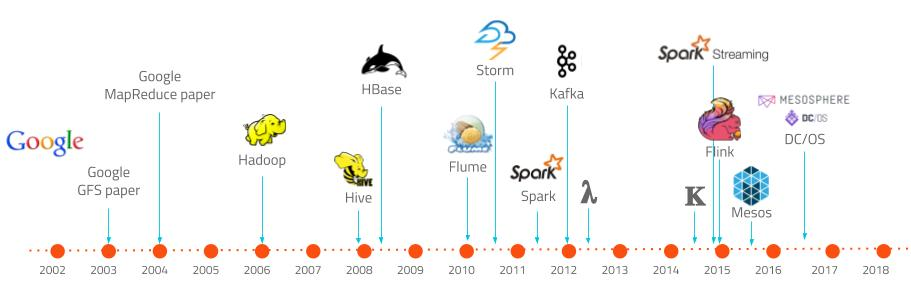
\includegraphics[width=0.94\textwidth]{images/arte/bigdatatime}
	\caption{Evolución del \textit{Big Data}. Fuente \cite{lambdakappa}}
	\label{fig:bigdatatime}
\end{figure}


Durante estos 10 años la popularidad de \textit{Hadoop} ha crecido exponencialmente y junto con las BBDD NoSQL, nacidas también a partir de Google con su BigTable, forman lo que hoy conocemos como Big Data. En la Figura \ref{fig:bigdatatime} observamos esta evolución en el mundo del \textit{Big Data} con los hitos de aparición de algunas tecnologías representativas.



El auge del \textbf{Big Data} ha llevado a algunas empresas a tener verdadera obsesión por el almacenamiento de todos los datos de sus clientes y las operaciones realizadas, creando inmensos \textit{datalakes} donde tener enormes históricos de todos sus datos. Este ``síndrome de Diógenes digital'' creado por falsas expectativas, por la imposibilidad de extraer valor de los datos o por la dimensión cambiante de las empresas actuales (en la que los datos de años atrás pueden no ser relevantes en el presente), es uno de los posibles motivos por lo que el tratamiento de los datos esta cambiando. Otro de los motivos para el cambio de rumbo del \textit{Big Data} está relacionado con la \textit{V} de Velocidad, hoy en día no solo es importante la capacidad de ingestar rápidamente los datos, sino la capacidad de poder procesar y obtener decisiones o actuar en tiempo real a partir de los datos, aportando valor al negocio. En este escenario se vuelve más importante la velocidad que el volumen de datos, esto es lo que se denomina \textit{Fast Data}. 



Dentro del \textit{Fast Data} es habitual el uso de BBDD \textit{in-memory}, de buses de eventos y de tecnologías de procesamiento capaces de procesar los eventos en tiempo real. Como veremos posteriormente al desarrollar nuestra arquitectura, el \textit{Fast Data} será una parte fundamental en nuestro proyecto en el que tendremos que clasificar las llamadas en tiempo real y tomar decisiones (o alarmar) en función de las mismas. 

Observando de nuevo la Figura \ref{fig:bigdatatime} podemos ver este cambio en la tendencia hacia el \textit{Fast Data} a partir del 2012 cuando aparece la tecnología Kafka y en los años posteriores con la incorporación de diferentes herramientas para el procesamiento de eventos como son \textit{Spark Streaming} o \textit{Flink}.

\subsection{Arquitecturas \textit{RealTime}}
La evolución que hemos visto en el apartado anterior,  con la explosión del \textit{Big Data} y la irrupción del \textit{Fast Data}, hace necesaria la incorporación en las empresas de arquitecturas de procesamiento de datos en tiempo real que, como cualquier otra arquitectura de datos, sean capaces de ingestar, procesar y permitir la explotación y análisis de los datos. La diferencia fundamental en las arquitecturas \textit{RealTime} y las arquitecturas de datos tradicionales son el\textbf{ volumen de los datos a tratar} y la \textbf{capacidad para hacerlo en tiempo real}.

Como veremos, no existe una arquitectura que se adapte a todos los casos de uso (\textit{one-size-fits-all}) y, según la necesidad, será necesario aplicar una u otra.

\subsubsection{Arquitectura Lambda $\lambda$}
La arquitectura lambda, representada por la letra griega $\lambda$, fue presentada en 2011 por Nathan Marz en un artículo publicado en su blog titulado ``\textit{How to beat the CAP theorem}'' \cite{lambda}.

\begin{figure}[!ht]
	\centering
	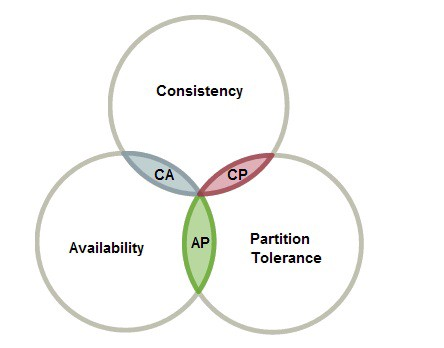
\includegraphics[width=0.55\textwidth]{images/arte/cap}
	\caption{Teorema CAP. Fuente \cite{cap}}
	\label{fig:cap}
\end{figure}

El propósito de Nathan Marz cuando crea su arquitectura, como indica el título del artículo, es batir el teorema CAP popularizado por la irrupción de las bases de datos NoSQL. Este teorema, ilustrado en la Figura \ref{fig:cap}, viene a decir que si queremos tener tolerancia a particiones (imprescindible para bases de datos distribuidas necesarias para el \textit{Big Data}), tenemos que optar entre consistencia, asegurar que el dato que leemos es el último que hemos escrito, o disponibilidad, que la base de datos se encuentra siempre lista.



El método propuesto para conseguir este objetivo con grandes cantidades de datos se basa en los siguientes principios:

\begin{itemize}
	\item Una capa \textit{batch} eventualmente consistente de una manera extrema, en la que las escrituras tardan siempre unas pocas horas en estar disponibles. Eliminando algunos problemas complejos con los que tratar como  la concurrencia o las reparaciones de lectura. 
	\item Reducir las operaciones CRUD (\textit{\textbf{C}reated, \textbf{R}ead, \textbf{U}pdate, \textbf{D}elete}) en la capa \textit{batch} por únicamente CR, tratando los datos como objetos inmutables. Esto nos soluciona el problema de la consistencia, ya que de este modo un dato existe o no existe, pero no puede tener varias versiones. 
	\item Una capa \textit{realtime} que se encarga de los datos de las últimas horas (los que no están disponibles en la capa \textit{batch})
	\item Las querys atacan a ambas capas de forma simultanea realizando un \textit{merge} de los datos.
	
\end{itemize}

\begin{figure}[!ht]
	\centering
	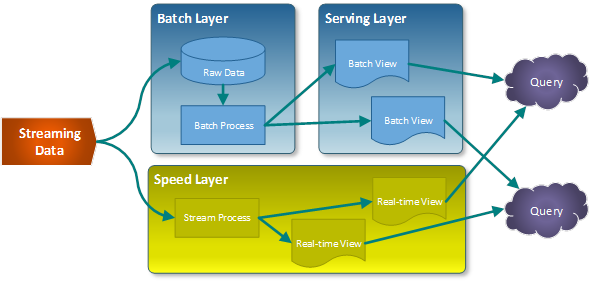
\includegraphics[width=0.70\textwidth]{images/arte/lambda}
	\caption{Arquitectura Lambda definida por   Nathan Marz. Fuente \cite{lambdakappa}}
	\label{fig:lambda}
\end{figure}


Podemos ver un esquema de la arquitectura en la Figura \ref{fig:lambda}. Esta arquitectura, aparte de resolver los problemas de consistencia y disponibilidad, tiene algunas ventajas:

\begin{itemize}
	
	\item Disponer de todos los datos en un único punto (capa \textit{batch}) pudiendo realizar cualquier tipo de consulta sobre los mismos. 
	\item Al utilizar los datos como un ente inmutable facilita las auditorias. 
	\item Según Marz, evita el error humano en la capa \textit{batch} (en parte también por usar datos inmutables), y cualquier error en la capa \textit{realtime} sería subsanado en pocas horas en la capa \textit{batch}.

\end{itemize}


\subsubsection{Arquitectura Kappa $\kappa$} 
\label{section:arte:big:arq} 
En su artículo ``Questioning the Lambda Architecture''\cite{kappa}, Jay Kreps cuestiona la arquitectura Lambda propuesta por Nathan Marz y propone una simplificación de la misma, basada en su experiencia en LinkedIn trabajando con Kafka y Samza. Esta simplificación se denomina arquitectura Kappa y viene representada por la letra griega $\kappa$.


Kreps describe la complejidad que supone en una arquitectura Lambda mantener idénticos procesos en \textit{realtime} y \textit{batch}. También expone que se menosprecia la capacidad de la capa \textit{realtime} (probablemente por la madurez del procesamiento \textit{realtime} con respecto al \textit{bacth}) y opina que es posible realizar el mismo procesamiento, incluso reprocesar el histórico de datos, en la capa \textit{realtime}. 

\begin{figure}[!ht]
	\centering
	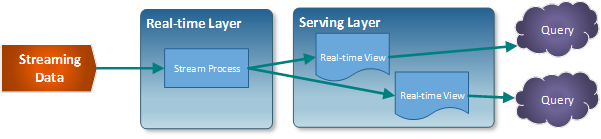
\includegraphics[width=0.70\textwidth]{images/arte/kappa}
	\caption{Arquitectura Kappa definida por Jay Kreps. Fuente \cite{lambdakappa}}
	\label{fig:kappa}
\end{figure}

Con esta premisa, en el artículo se presenta la arquitectura que observamos en la Figura \ref{fig:kappa}, en la que existe un único flujo de procesamiento \textit{realtime} para todo el modelo. La simplicidad de Kappa con respecto a Lambda es tal que el propio Kreps afirma que puede ser una idea demasiado simple para merecer una letra griega.



\section{Trabajos anteriores}
\label{section:arte:ant}


Una vez abordado el estado del arte desde diferentes puntos de vista, es importante tener una visión de los trabajos anteriores que se han realizado con objetivos similares y sus resultados. De este modo entenderemos si existe una justificación para nuestro trabajo, los problemas a los que podemos enfrentarnos y las expectativas que podemos gestionar.

En este apartado nos vamos a  centrar en la aplicación de técnicas de Procesamiento del Lenguaje Natural a un \textit{Call Center}. Encontramos varios artículos interesantes que hacen hincapié en el valor de la información y el conocimiento que puede extraerse de un \textit{Call Center}, ya que se trata de un intermediario importante entre el cliente y la empresa. Entre estos trabajos podemos destacar: 

\begin{itemize}
	\item ``Metodología para estimar el impacto que generan las llamadas realizadas en un call center en la fuga de los clientes utilizando técnicas de text mining'' \cite{call1}: Que como su nombre indica, investiga si existe relación entre las llamadas realizadas al \textit{Call Center} y la pérdida de clientes. El trabajo, al igual que el proyecto que intentamos abordar, parte de las llamadas transcritas a texto y, aunque se utiliza como base para la modelización de temas LDA, se apoya en etiquetas existentes en las llamadas para validar los resultados.
	
	\item ``Customer voice sensor: A comprehensive opinion mining system for call center conversation'' \cite{call2}: Se trata de un trabajo más basado en el análisis de sentimientos, pero se encuentra realizado con llamadas de los clientes a una operadora de telecomunicaciones (en este caso China Telecom) al igual que nuestra fuente de información.
	
	\item ``Topic mining for call centers based on A‐LDA and distributed computing'' \cite{call3}: En este caso, se realiza una modelización de temas sobre  los datos del \textit{Call Center} de \textit{China Central Television}. En este proceso de modelización se utiliza  una mejora del modelo LDA llamada A-LDA que utiliza no solo el corpus de la llamada, si no también algunas propiedades externas como el tiempo de llamada o el número de origen.
	
	\item ``Author-topic based representation of call-center conversations'' \cite{call4}: Este último artículo que comentamos, parte también de los datos generados a través de un \textit{Performance of Automatic Speech Recognition} (ASR), el trabajo pone de manifiesto la pobre calidad de estas transcripciones automáticas. Por este motivo, propone una modificación de LDA basada en el modelo \textit{Author Topic}, utilizando además del corpus del texto información del tema de la conversación.
\end{itemize}


Probablemente, dentro de las empresas, existen muchos más trabajos destinados a la explotación de esta información y que no se encuentren publicados, por lo que podemos concluir que es un campo que despierta interés y que se trata de una información con potencial que nos permita, entre otros objetivos, comprender las necesidades de los clientes de una compañía.

Por otro lado, observamos que en la mayoría de los casos, aunque la base de la modelización sea el uso de LDA, debido al ruido o a otros factores como la ausencia de información semántica, se utilizan modificaciones del modelo que incorporan etiquetas o propiedades externas al corpus para mejorar la clasificación.

Por último, pensamos que, aún con estos antecedentes, existe la necesidad de abordar este proyecto, debido a la diferencia entre unos datos y otros, por factores como el idioma o las distintas necesidades de cada empresa. Además nuestro proyecto tiene como objetivo final la integración de este modelo en un proceso de la compañía que sea capaz de aplicarlo en tiempo real y alertar en caso de anomalías para poder tomar decisiones.


\chapter{Arquitectura y tecnologías}
\label{chapter:arquitectura}

El objetivo de este capítulo es tener una visión global de lo que será nuestro proyecto, antes de entrar en más profundidad en cada una de las partes. El proyecto que presentamos en este documento consta de dos partes bien diferenciadas. Por un lado, una parte que podemos considerar ``de laboratorio'', en la que realizaremos las labores más analíticas sobre los datos disponibles: extracción, procesamiento, estudio y creación de modelos; la cuál presentamos en la sección \ref{section:arq:mod}. Y por otro lado, una parte ``de explotación'', en la que trataremos de poner en valor los resultados de la primera parte en el mundo real y que será tratada en la sección \ref{section:arq:exp}. 


El capítulo se completará con la sección \ref{section:arq:mant}, dedicada al mantenimiento del proyecto una vez llevado a producción y con la sección \ref{section:arqu:tecn}, en la que se describirán a grandes rasgos todas la tecnologías usadas en el proyecto.





\section{Modelado}
\label{section:arq:mod}
La primera parte de nuestro proyecto pretende conseguir el objetivo principal propuesto en  la sección \ref{section:intro:objetivos}, \textbf{clasificar las llamadas}. Para ello tendremos que analizar y entender los datos que poseemos de las transcripciones y posteriormente construir los modelos necesarios (supervisados o no supervisados) que nos permitan clasificar las llamadas.

Para lograr este objetivo necesitaremos disponer de un \textit{datalake} en el que se almacene todo el histórico de transcripciones de las llamadas, ya que para el entrenamiento de muchos modelos será necesario utilizar un amplio histórico para su entrenamiento. Este \textit{datalake} será un sistema de archivos HDFS perteneciente a una plataforma Hadoop Hortonworks. El procedimiento de carga de las transcripciones en HDFS se encuentra ya realizado y queda fuera del alcance del proyecto. Debido a que no tenemos ningún requisito temporal para la ingesta de las transcripciones, este no será un elemento crítico de nuestro proyecto. 

En cuanto a la plataforma que utilizaremos para realizar la analítica, puede ser independiente del entorno de almacenamiento siempre que podamos transferir los datos a la misma. A lo largo del proyecto hemos trabajado con dos entornos diferentes: 

\begin{itemize}
\item Entorno \textbf{Spark}: Ubicado en un clúster Hadoop Hortonworks, nos ha permitido procesar grandes cantidades de datos en un espacio de tiempo muy reducido, gracias a los beneficios de la programación distribuida. Sin embargo, no se trata del entorno ideal para el entrenamiento de modelos, principalmente para modelos  \textit{deep learning}.

\item Entorno \textbf{GPU}s: Una única máquina con diferentes \textit{GPU}s NVIDIA. Este entorno nos ha permitido entrenar los modelos de \textit{deep learning} con una rapidez pasmosa (comparado con los entornos con CPUs). Ha sido la plataforma principal de analítica durante este proyecto, aunque el preprocesado se viera penalizado con respecto al entorno Spark.


\end{itemize}
 

El modelo presentado en nuestra arquitectura es un elemento sometido al cambio y, además de por posibles mejoras en los hiperparámetros o por la tecnología, debe re-entrenarse conforme se vayan recibiendo datos nuevos en el histórico, ya que es lógico pensar que la temática de las consultas variarán a lo largo del tiempo debido por ejemplo al lanzamiento de nuevos productos. 


En los capítulos \ref{chapter:dataset}, \ref{chapter:nosup} y \ref{chapter:super} trataremos en más detalle toda la parte de modelado, desde el análisis de los datos hasta la creación de modelos supervisados y no supervisados.

\section{Explotación}
\label{section:arq:exp}
La segunda parte del proyecto tendrá como meta llevar a producción el resultado de la etapa de modelado. Teniendo en cuenta que uno de nuestros objetivos consiste en clasificar las llamadas en tiempo real,
el primer paso que debemos abordar es seleccionar un modelo de arquitectura de procesamiento en tiempo real de entre las opciones vistas en la sección \ref{section:arte:big:arq}: Lambda y Kappa. Lo que intentamos en este paso, ya que no existe una solución ideal que se adapte a todos los casos de uso, es encontrar la solución que mejor se adapte a nuestro proyecto.


En nuestro caso, disponemos de todas las llamadas en tiempo real, que nos llegarán en forma de eventos. Además cada llamada podrá ser tratada de forma individual y no debemos preocuparnos por eventos que lleguen con retraso. Estos son los motivos principales que nos han llevado a decidirnos por la arquitectura Kappa propuesta por Jey Kreps, debido a la mayor simplicidad tanto a la hora de elaborar la capa de servicio, como a la hora de mantener un único desarrollo \textit{real-time}. 






En la figura \ref{fig:kappa2} podemos ver la arquitectura global de la solución propuesta. Esta arquitectura consta de dos capas principales. Por un lado, una capa de \textit{streaming} o capa rápida donde se realizará todo el procesamiento en \textit{streaming} de las transcripciones de las llamadas conforme vayan llegando. Por otro lado, una capa de servicio que permite a los usuarios explotar la información procesada en la primera capa. 



\begin{figure}[!ht]
	\centering
	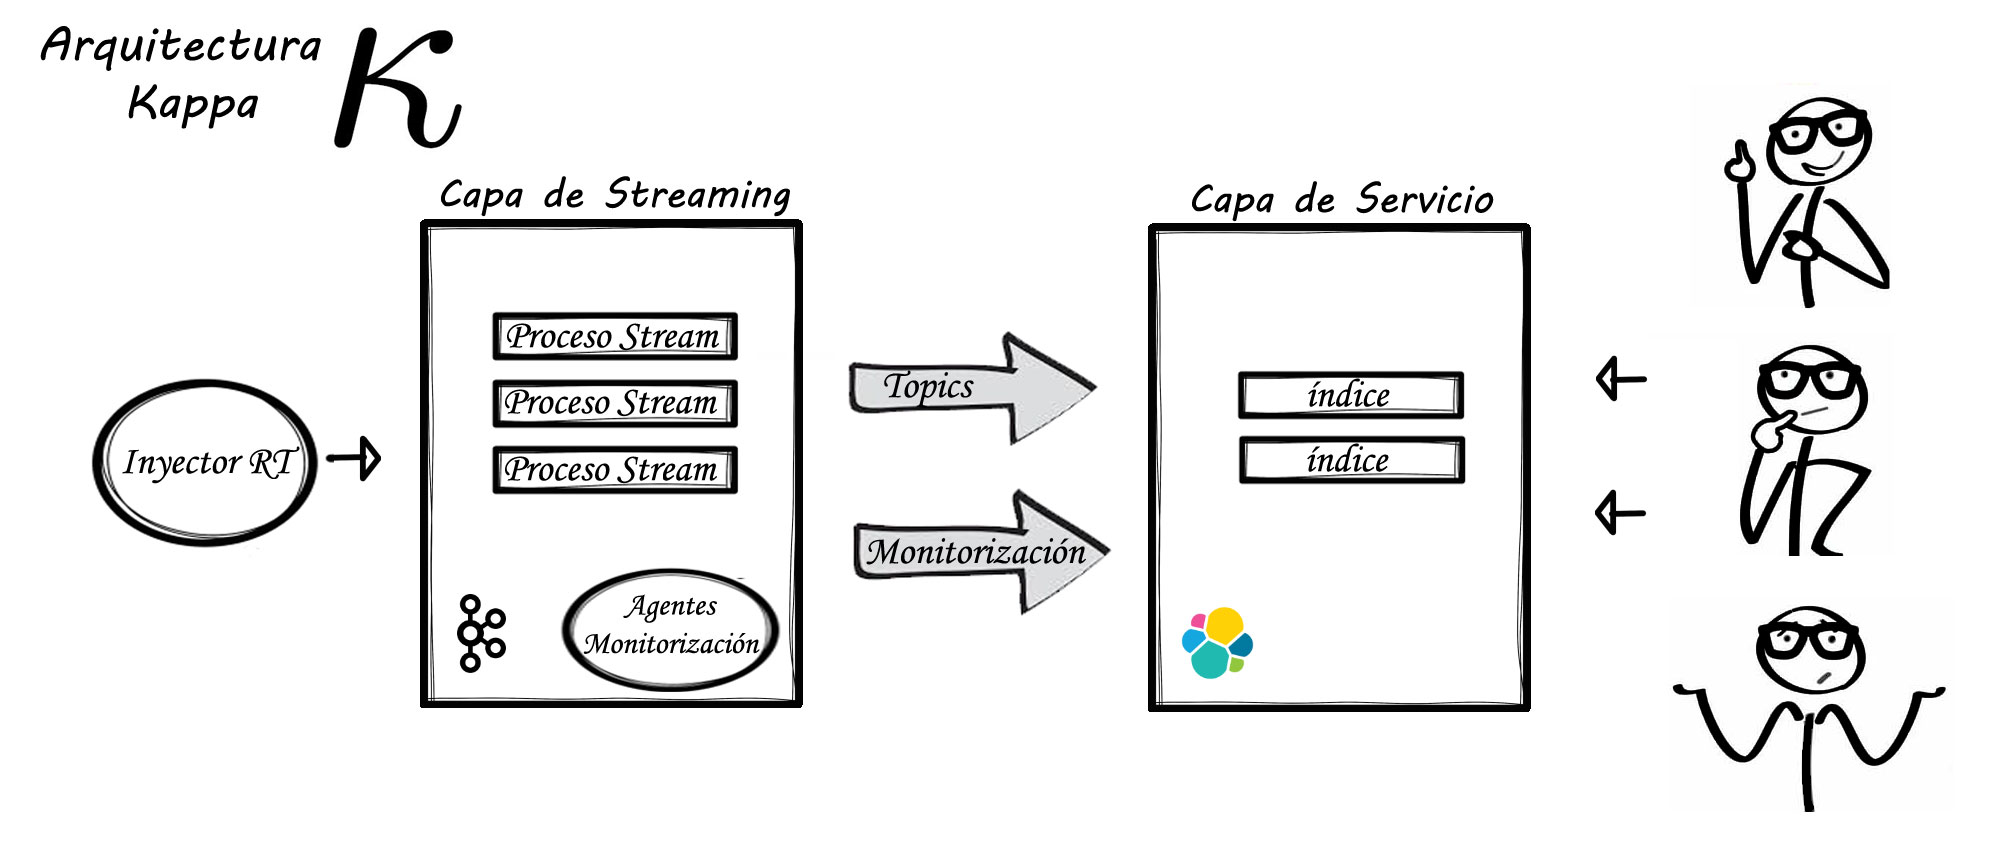
\includegraphics[width=1\textwidth]{images/arqu/kappa_v1}
	\caption{Arquitectura Kappa}
	\label{fig:kappa2}
\end{figure}


El \textit{core} de la primera capa será Apache Kafka, que además nos dará la posibilidad de retener los eventos y poder reprocesarlos en caso de error, siendo una solución ideal para arquitecturas Kappa. De hecho Jey Kreps, quien propuso la arquitectura Kappa es el co-fundador de Confluent, la compañía que se encuentra detrás de Apache Kafka. Los detalles de la capa de \textit{streaming} podemos verlos con más detalle en el capítulo \ref{chapter:prod}.

El núcleo de la capa de servicio será el \textit{stack} de Elastic. Esta solución nos permitirá ingestar los eventos desde la capa rápida en tiempo real y exponerlos a los usuarios. Además usaremos este mismo flujo para todos los eventos de monitorización. El hecho de utilizar el \textit{stack} de Elastic nos dará posibilidad de realizar el alarmado estático y dinámico en esta misma capa.  Los detalles de esta capa se describen en detalle en el capítulo \ref{chapter:servicio}. 




Debido a la situación actual, las llamadas no se ingestan en \textit{real-time} si no que se reciben mediante procesos \textit{batch} cada cierto tiempo. Este escenario cambiará en el futuro por lo que se construirá un elemento de entrada a la capa rápida que actúe como inyector, generando eventos en tiempo real a partir de los datos en \textit{batch}. Esta pieza será suprimida una vez las llamadas sean recibidas en tiempo real. 



\section{Mantenimiento e Integración Continua}
\label{section:arq:mant}

Como ya hemos visto al hablar del entrenamiento del modelo, el desarrollo de este tipo de proyectos no tiene un principio y un final, si no que se trata de un proceso cíclico en el que por necesidades del negocio, por cambio en los datos o por cambio en las tecnologías, será necesario añadir mejoras o modificaciones en nuestro desarrollo. También el despliegue del \textit{software} en producción es un proceso susceptible de futuros cambios.  



Por estos motivos será necesario disponer de algún método para seguir evaluando la calidad del modelo una vez sea llevado a producción,  tener la posibilidad de realizar test A/B en el futuro, y  definir mecanismos que nos permitan, tras cada cambio efectuado, poder realizar las pruebas necesarias y desplegar estos cambios de una manera totalmente automatizada y sin intervención humana.

Para conseguir estos objetivos, con la mayor agilidad posible, será necesario trabajar en un marco de trabajo \textit{DevOps} contando con mecanismos que nos permitan realizar tanto integración, como despliegue continuos.  En el capítulo \ref{chapter:mant} veremos con más detalle como aplicamos esta metodología.





\section{Tecnologías}
\label{section:arqu:tecn}
Al igual que la arquitectura descrita anteriormente era la encargada de responder a las necesidades de negocio, las tecnologías descritas en este apartado nos darán las piezas necesarias para poder construir esa arquitectura y dar respuesta a nuestro caso de uso. 


En el proceso de selección de las tecnologías, no solo se ha tenido en cuenta la idoneidad de las mismas para el caso de uso, si no que se ha valorado también la experiencia en la misma y la disponibilidad dentro del entorno de trabajo. Esto puede provocar que en algunos casos aunque la tecnología se adapte al caso de uso, puedan existir otras soluciones más óptimas cuyo uso era menos viable, dados los plazos de ejecución del proyecto. 

A continuación enumeraremos las tecnologías agrupadas en las diferentes capas que hemos comentado en el apartado de arquitectura, además añadiremos las tecnologías que se usarán para la integración y despliegue continuo. 

\subsection{Modelado}


La parte de modelado la realizaremos trabajando siempre con Python 3.6 y Jupyter, trabajar en un entorno dinámico e interactivo mediante \textit{notebooks} nos dará mucha flexibilidad para poder realizar nuestro análisis.

A continuación vemos las bibliotecas más relevantes que hemos usado, tanto en entorno Spark como en el entorno de GPUs.


\begin{itemize}
	

%	\item \textbf{Spark}: Es un framework de computación en clúster. Este \textit{framework} se encuentra desplegado sobre un clúster Hadoop, específicamente una distribución HortonWorks, y posee librerías específicas para Machine Learning como MLLIB.
%	\item \textbf{Tensorflow} sobre GPUs: Para el entrenamiento de los modelos también disponemos de un cluster con GPUs sobre el que podremos correr código usando la librería de Google Tensorflow para entrenar nuestros modelos.
\item \textbf{Spark SQL y \textit{dataframes}}: Dentro del entorno de Spark, para el procesamiento de los datos trabajaremos con las bibliotecas de Spark SQL y \textit{dataframes}, que nos permitirán de una manera sencilla realizar transformaciones en nuestros datos de forma distribuida.
\item \textbf{MLlib}: También en el entorno de Spark usaremos la biblioteca nativa MLlib, que nos permite crear algoritmos y modelos de \textit{machine learning} sobre un cluster Spark.
\item \textbf{Pandas}: Al igual que en \textit{Spark} utilizamos las bibliotecas de SQL y \textit{dataframes}, Pandas nos permitirá hacer el análisis y manipulación de los datos en cualquier entorno Python.
\item \textbf{ Keras}: Será la biblioteca que usaremos, con  \textbf{Tensorflow} como backend, para crear modelos de \textit{deep learning}.

\item \textbf{Gensim}: Se trata de una biblioteca para el modelado de temas no supervisados y el procesamiento del lenguaje natural.

\item \textbf{NLTK}: Son un conjunto de bibliotecas que nos ayudarán a realizar tareas de procesamiento de lenguaje natural.
\item \textbf{Sklearn}: Se trata de una biblioteca para tareas de \textit{machine learning}, que contiene multitud de funciones que nos ayudarán en nuestro desarrollo.
	
	
\item \textbf{Optuna}:	 Por último, la biblioteca Optuna nos ayudará a optimizar los modelos supervisados que creemos. Hablaremos de ella con más detalle en la sección \ref{section:super:opt}.
	
	
\end{itemize}

\subsection{Explotación}

A continuación veremos las tecnologías y plataformas que harán posible el despliegue de nuestra capa de \textit{streaming}. Estas tecnologías serán vistas con más detalle a lo largo del capítulo \ref{chapter:prod}.

\begin{itemize}
	\item \textbf{Apache Kafka}: Es el \textit{core} de la capa rápida, se trata de un bus de eventos distribuidos, a través del cual se realizará la ingesta o publicación de los eventos (llamadas). Las diferentes capas de procesamiento que requieran estos eventos se suscribirán a este Bus.
	%\item \textbf{Microservicios}: En nuestra capa Real Time construiremos diferentes microservicios en la capa de procesamiento, estos microservicios serán por ejemplo los encargados de devolver los \textit{topics} de cada llamada a partir de una llamada API REST. Estos microservicios correran sobre contenedores en una plataforma Openshift.
	
	
	\item \textbf{Tensorflow Serving}: Servicio para servir modelos de \textit{machine learning} creado dentro del ecosistema Tensorflow.
	\item \textbf{Kafka Stream}: A la hora de procesar la información en eventos ingestada en nuestro Bus Kafka disponemos de Kafka Stream. Una serie de bibliotecas que nos permiten construir aplicaciones y microservicios cuyo origen y destino sean un Bus Kafka. 
	
	\item  \textbf{ Openshift}: Se trata de una plataforma de contenedores de Kubernetes creada por \textit{Red Hat}. Todos los desarrollos de la capa de explotación serán implementados sobre contenedores.

	
\end{itemize}

\subsection{Capa Servicio}

La capa de servicio estará compuesta, como hemos indicado, por el \textit{stack} de Elastic. Este \textit{stack} posee diferentes piezas, cada una de las cuales realiza una función determinada. 

\begin{itemize}

	\item \textbf{Elasticsearch}: Se trata del núcleo del \textit{stack}. Aunque no se trata en el sentido más estricto de una BBDD No-SQL, si no de un motor de búsqueda, Elasticsearch nos permite almacenar la información en forma de documentos json en tiempo real y realizar consultas y agregaciones sobre cualquier campo. Entre las características que podemos aprovechar de Elasticsearch para nuestro objetivo están: 
		\begin{itemize}
			\item Ingesta en tiempo real.
			\item Consulta en tiempo real. 
			\item Disponibilidad de mecanismos de ingesta (Logstash) y consulta (Kibana).
			\item Posibilidad de crear alarmas en base a consultas. 
			\item Posibilidad de crear \textit{jobs} de \textit{machine learning} que detecten anomalías en series temporales. 
			\item API REST: Posibilidad de realizar cualquier operación o consulta mediante API REST.
		\end{itemize}



	\item \textbf{Logstash}: Será la pieza que nos permitirá transportar la información desde la capa de \textit{streaming} a la capa de servicio. Logstash nos permitirá leer de Apache Kafka, realizar las transformaciones necesarias y volcar la información resultante en Elasticsearch. Además de los datos propios de la clasificación, Logtsash nos ayudará a extraer también los datos de monitorización de la capa de Streaming.
	
	\item \textbf{Kibana}: Será el frontal donde los usuarios podrán consultar sus diferentes cuadros de mando y construir nuevos de acuerdo a sus necesidades. También, gracias al módulo de \textit{machine learning} de Elasticsearch, los usuarios podrán crear \textit{jobs} de \textit{machine learning} para detectar anomalías en los temas tratados y generar las alertas necesarias.
	
	
	\item \textbf{Beats}: Se trata de agentes ligeros que nos permitirán extraer información variada de distintas fuentes. En nuestro caso usaremos \textit{Metricbeat} para extraer datos de monitorización de la capa de \textit{streaming}. 
	
	
	
		
	
		
\end{itemize}





\subsection{Integración y Despliegue Continuo}

Por último, para conseguir los objetivos de integración y despliegue continuos utilizaremos diversas  tecnologías. Estas tecnologías, y la interacción entre ellas se verán con más detalle en el capítulo \ref{chapter:mant}.

\begin{itemize}
	\item \textbf{BitBucket}: Será el repositorio usado para almacenar las nuevas versiones de nuestro \textit{software} de manera que podamos tener un control de versiones. Almacenará tanto el código de nuestra capa de \textit{streaming}, como de los modelos que necesitemos poner en producción. 
	\item \textbf{Jenkins}: Es un servidor de integración continua \textit{open source}  que, mediante la creación de tareas, nos ayudará a realizar el \textit{build} de nuestro software realizando de manera automática las pruebas necesarias.
	\item \textbf{Nexus}: Se trata de un gestor de repositorios, en nuestro caso utilizaremos repositorios de Maven. Es usual usar este tipo de gestores de repositorios en las empresas para disponer de bibliotecas propias (y no públicas) y para no tener una dependencia con ningún agente externo.
	\item \textbf{S2I}: Se trata de una funcionalidad de Openshift que será vital para el desarrollo del despliegue continuo. Esta funcionalidad nos permitirá crear nuevas imágenes de contenedores a partir de código o binarios propios.
\end{itemize}












\part{Modelado: datos, modelos y optimizaciones}
\chapter{Conjunto de datos}
\label{chapter:dataset}
El primer paso cuando nos enfrentamos a un problema de minería de datos, es comprender el conjunto de datos con el que contamos y ver si se adapta a nuestras necesidades. En este caso, al tratarse de un proyecto que se desarrolla dentro de una empresa, en caso de duda, hemos tenido la posibilidad de acudir a las áreas dueñas del dato para solicitarle información adicional sobre el mismo. 


En este capítulo abordaremos todos los aspectos relacionados con los datos que hemos ido recopilando durante el desarrollo del proyecto. En la sección \ref{section:data:ana}, describiremos el conjunto de datos con el que hemos estado trabajando, posteriormente en la sección \ref{section:data:repr} veremos las diferentes formas que hemos usado para representar los datos que alimentan los modelos que hemos construido (y que describiremos en los siguientes capítulos) y, por último, en la sección \ref{section:data:evol} echaremos la vista atrás para ver el conjunto de datos inicial y poder apreciar la evolución que ha ido sufriendo.


Otro de los objetivos del capítulo es poner de manifiesto la importancia de la parte quizás menos ``glamurosa'' que está presente en todos los proyectos de minería de datos. Cuando exponemos un proyecto de minería de datos siempre ponemos el foco en los modelos creados, sin embargo, el grueso del trabajo en los proyectos de este tipo se encuentra en recopilar datos, entenderlos y preprocesarlos (o limpiarlos). Todo este proceso es el que intentaremos describir en las siguientes páginas.


En el código expuesto a lo largo del capítulo se hará referencia a un módulo llamado \textit{mgmtfm}, se trata de de un módulo en \textit{Python} creado especialmente para este proyecto y que nos permitirá realizar las tareas necesarias con un nivel de abstracción mayor. 

\section{Análisis del conjunto de datos}
\label{section:data:ana}
En este apartado analizaremos el conjunto de datos con el que trabajaremos a lo largo de todo el documento. Como veremos en el apartado \ref{section:data:evol}, este conjunto de datos ha sido fruto de un proceso evolutivo y de recopilar información de diferentes fuentes. 

El resto de esta sección de análisis lo dividiremos en secciones como si se tratara de un \textit{notebook} de \textit{Jupyter}, que ha sido la interfaz utilizada para realizar el análisis.


\subsection{Imports}

   Importamos las librerías y establecemos los parámetros que necesitaremos en la ejecución del \textit{notebook}.

\vspace{0.5cm}

    \begin{tcolorbox}[breakable, size=fbox, boxrule=1pt, pad at break*=1mm,colback=cellbackground, colframe=cellborder]
\prompt{In}{incolor}{1}{\boxspacing}
\begin{Verbatim}[commandchars=\\\{\}]
\PY{k+kn}{import} \PY{n+nn}{sys}
\PY{n}{sys}\PY{o}{.}\PY{n}{path}\PY{o}{.}\PY{n}{append}\PY{p}{(}\PY{l+s+s2}{\PYZdq{}}\PY{l+s+s2}{..}\PY{l+s+s2}{\PYZdq{}}\PY{p}{)}
\PY{k+kn}{import} \PY{n+nn}{warnings}
\PY{n}{warnings}\PY{o}{.}\PY{n}{filterwarnings}\PY{p}{(}\PY{l+s+s1}{\PYZsq{}}\PY{l+s+s1}{ignore}\PY{l+s+s1}{\PYZsq{}}\PY{p}{)}
\PY{k+kn}{import} \PY{n+nn}{pandas} \PY{k}{as} \PY{n+nn}{pd}
\PY{k+kn}{import} \PY{n+nn}{numpy} \PY{k}{as} \PY{n+nn}{np}
\PY{k+kn}{from} \PY{n+nn}{datetime} \PY{k}{import} \PY{n}{datetime}
\PY{k+kn}{import} \PY{n+nn}{nltk}
\PY{k+kn}{from} \PY{n+nn}{nltk}\PY{n+nn}{.}\PY{n+nn}{tokenize}\PY{n+nn}{.}\PY{n+nn}{toktok} \PY{k}{import} \PY{n}{ToktokTokenizer}
\PY{k+kn}{from} \PY{n+nn}{nltk}\PY{n+nn}{.}\PY{n+nn}{corpus} \PY{k}{import} \PY{n}{stopwords}
\PY{k+kn}{from} \PY{n+nn}{mgmtfm} \PY{k}{import} \PY{n}{clean}
\PY{k+kn}{from} \PY{n+nn}{wordcloud} \PY{k}{import} \PY{n}{WordCloud}
\PY{k+kn}{import} \PY{n+nn}{matplotlib}\PY{n+nn}{.}\PY{n+nn}{pyplot} \PY{k}{as} \PY{n+nn}{plt}


\PY{n}{pd}\PY{o}{.}\PY{n}{set\PYZus{}option}\PY{p}{(}\PY{l+s+s1}{\PYZsq{}}\PY{l+s+s1}{max\PYZus{}rows}\PY{l+s+s1}{\PYZsq{}}\PY{p}{,}\PY{l+m+mi}{9999}\PY{p}{)}
\PY{n}{pd}\PY{o}{.}\PY{n}{set\PYZus{}option}\PY{p}{(}\PY{l+s+s1}{\PYZsq{}}\PY{l+s+s1}{max\PYZus{}columns}\PY{l+s+s1}{\PYZsq{}}\PY{p}{,} \PY{l+m+mi}{9999}\PY{p}{)}
\PY{n}{pd}\PY{o}{.}\PY{n}{set\PYZus{}option}\PY{p}{(}\PY{l+s+s1}{\PYZsq{}}\PY{l+s+s1}{display.max\PYZus{}colwidth}\PY{l+s+s1}{\PYZsq{}}\PY{p}{,} \PY{l+m+mi}{500}\PY{p}{)}


\PY{n+nb}{print}\PY{p}{(}\PY{l+s+s2}{\PYZdq{}}\PY{l+s+s2}{Notebook ejecutado el }\PY{l+s+si}{\PYZob{}\PYZcb{}}\PY{l+s+s2}{.}\PY{l+s+s2}{\PYZdq{}}\PY{o}{.}\PY{n}{format}\PY{p}{(}\PY{n}{datetime}\PY{o}{.}\PY{n}{now}\PY{p}{(}\PY{p}{)}\PY{o}{.}\PY{n}{strftime}\PY{p}{(}\PY{l+s+s2}{\PYZdq{}}\PY{l+s+si}{\PYZpc{}d}\PY{l+s+s2}{\PYZhy{}}\PY{l+s+s2}{\PYZpc{}}\PY{l+s+s2}{m\PYZhy{}}\PY{l+s+s2}{\PYZpc{}}\PY{l+s+s2}{Y}\PY{l+s+s2}{\PYZdq{}}\PY{p}{)}\PY{p}{)}\PY{p}{)}
\end{Verbatim}
\end{tcolorbox}

    \begin{Verbatim}[commandchars=\\\{\}]
Using TensorFlow backend.
    \end{Verbatim}

    \begin{Verbatim}[commandchars=\\\{\}]
Notebook ejecutado el 12-11-2019.
    \end{Verbatim}

    \hypertarget{carga-de-datos}{%
\subsection{Carga de datos}\label{carga-de-datos}}

    El \textit{core} de nuestros datos son las llamadas en sí. Actualmente disponemos de grabaciones de un 20\% de las llamadas de las que se transcriben un
20\% (lo que supone un 4\% del total), estas llamadas llegan a nuestra plataforma de análisis mediante un
proceso \textit{batch}. El objetivo es disponer en un futuro del 100\% de las
transcripciones en tiempo real.

Para comenzar el análisis, cargamos el \textit{dataset}.

\vspace{0.5cm}

    \begin{tcolorbox}[breakable, size=fbox, boxrule=1pt, pad at break*=1mm,colback=cellbackground, colframe=cellborder]
\prompt{In}{incolor}{2}{\boxspacing}
\begin{Verbatim}[commandchars=\\\{\}]
\PY{n}{verint\PYZus{}raw} \PY{o}{=} \PY{n}{pd}\PY{o}{.}\PY{n}{read\PYZus{}parquet}\PY{p}{(}\PY{l+s+s1}{\PYZsq{}}\PY{l+s+s1}{/data/datasets/input\PYZus{}data/verint\PYZus{}dataset.parquet}\PY{l+s+s1}{\PYZsq{}}\PY{p}{)}
\end{Verbatim}
\end{tcolorbox}

        
 Describimos brevemente los campos que pueden ser de utilidad para nuestro proyecto: 
 
 \begin{itemize}


\item \textbf{\textit{co\_llamada\_verint}}: Código de la llamada en el sistema, nos servirá
para identificar de manera unívoca la transcripción.

 \item \textbf{\textit{ucid}}: Código unívoco de la llamada.

\item \textbf{\textit{fx\_evento}}: Fecha del evento.

\item \textbf{\textit{it\_llamada}}: Timestamp del evento.

\item \textbf{\textit{datecreated}}: Timestamp en el que se crea la transcripción.

\item \textbf{\textit{plaintext}}: Transcripción de la llamada en texto plano.

\item \textbf{\textit{audio\_start\_time}}: Hora de inicio del audio. Formato UTC.

\item \textbf{\textit{cd22}}: Provincia desde la que se ha realizado la llamada. 

\item \textbf{\textit{no\_destino\_pa}}: Código IVR que categoriza la llamada en función de las
opciones que elige el usuario al llamar.

\item \textbf{\textit{duration}}: Duración de la llamada.


 \end{itemize}

Aunque existen más campos en el conjunto de datos original, estos no son relevantes para 
nuestro caso de uso.

    Utilizamos  un subconjunto de estos campos, para realizar un análisis
previo. Vemos en primer lugar el número total de llamadas disponibles:
\vspace{0.5cm}

    \begin{tcolorbox}[breakable, size=fbox, boxrule=1pt, pad at break*=1mm,colback=cellbackground, colframe=cellborder]
\prompt{In}{incolor}{3}{\boxspacing}
\begin{Verbatim}[commandchars=\\\{\}]
\PY{n}{verint} \PY{o}{=} \PY{n}{verint\PYZus{}raw}\PY{p}{[}\PY{p}{[}\PY{l+s+s1}{\PYZsq{}}\PY{l+s+s1}{co\PYZus{}llamada\PYZus{}verint}\PY{l+s+s1}{\PYZsq{}}\PY{p}{,}\PY{l+s+s1}{\PYZsq{}}\PY{l+s+s1}{ucid}\PY{l+s+s1}{\PYZsq{}}\PY{p}{,}\PY{l+s+s1}{\PYZsq{}}\PY{l+s+s1}{fx\PYZus{}evento}\PY{l+s+s1}{\PYZsq{}}\PY{p}{,}\PY{l+s+s1}{\PYZsq{}}\PY{l+s+s1}{it\PYZus{}llamada}\PY{l+s+s1}{\PYZsq{}}\PY{p}{,}
                     \PY{l+s+s1}{\PYZsq{}}\PY{l+s+s1}{duration}\PY{l+s+s1}{\PYZsq{}}\PY{p}{,} \PY{l+s+s1}{\PYZsq{}}\PY{l+s+s1}{plaintext}\PY{l+s+s1}{\PYZsq{}}\PY{p}{,} \PY{l+s+s1}{\PYZsq{}}\PY{l+s+s1}{no\PYZus{}destino\PYZus{}pa}\PY{l+s+s1}{\PYZsq{}}\PY{p}{]}\PY{p}{]}
\PY{n}{verint}\PY{o}{.}\PY{n}{plaintext} \PY{o}{=} \PY{n}{verint}\PY{o}{.}\PY{n}{plaintext}\PY{o}{.}\PY{n}{str}\PY{o}{.}\PY{n}{lower}\PY{p}{(}\PY{p}{)}
\PY{n+nb}{print}\PY{p}{(}\PY{n}{verint}\PY{o}{.}\PY{n}{count}\PY{p}{(}\PY{p}{)}\PY{p}{)}
\end{Verbatim}
\end{tcolorbox}

    \begin{Verbatim}[commandchars=\\\{\}]
co\_llamada\_verint    509374
ucid                 509374
fx\_evento            509374
it\_llamada           508524
duration               3457
plaintext            509374
no\_destino\_pa        508497
dtype: int64
    \end{Verbatim}


        
    \hypertarget{monitorizaciones}{%
\subsubsection{Monitorizaciones}\label{monitorizaciones}}

    Otra fuente de datos de la  que disponemos, son las monitorizaciones de las
llamadas. Se trata de un cuestionario realizado por un grupo de personas
sobre llamadas escuchadas. A nosotros nos interesa la parte relacionada
con el tipo de la llamada, que viene identificada en el cuestionario con los
prefijos $C$ y $D$.

\vspace{0.5cm}


    \begin{tcolorbox}[breakable, size=fbox, boxrule=1pt, pad at break*=1mm,colback=cellbackground, colframe=cellborder]
\prompt{In}{incolor}{4}{\boxspacing}
\begin{Verbatim}[commandchars=\\\{\}]
\PY{n}{monitorizaciones} \PY{o}{=} \PY{n}{pd}\PY{o}{.}\PY{n}{read\PYZus{}parquet}\PY{p}{(}\PY{l+s+s1}{\PYZsq{}}\PY{l+s+s1}{/data/datasets/input\PYZus{}data/monitorizaciones.parquet}\PY{l+s+s1}{\PYZsq{}}\PY{p}{)}
\PY{n+nb}{print}\PY{p}{(}\PY{l+s+s2}{\PYZdq{}}\PY{l+s+s2}{Tenemos }\PY{l+s+si}{\PYZob{}:,\PYZcb{}}\PY{l+s+s2}{ llamadas monitorizadas.}\PY{l+s+s2}{\PYZdq{}}\PY{o}{.}\PY{n}{format}\PY{p}{(}\PY{n+nb}{len}\PY{p}{(}\PY{n}{np}\PY{o}{.}\PY{n}{unique}\PY{p}{(}\PY{n}{monitorizaciones}\PY{p}{[}\PY{l+s+s2}{\PYZdq{}}\PY{l+s+s2}{ucid}\PY{l+s+s2}{\PYZdq{}}\PY{p}{]}\PY{p}{)}\PY{p}{)}\PY{p}{)}\PY{p}{)}
\end{Verbatim}
\end{tcolorbox}

    \begin{Verbatim}[commandchars=\\\{\}]
Tenemos 45,465 llamadas monitorizadas.
    \end{Verbatim}

        
    Al igual que hemos hecho anteriormente, vemos los datos más relevantes
de este Dataset:

\begin{itemize}
 


\item \textbf{\textit{co\_llamada\_verint}}: Código de la llamada en el sistema, nos servirá
para identificar de manera unívoca la transcripción.

\item \textbf{\textit{ucid}}: Código unívoco de la llamada.

\item \textbf{\textit{it\_llamada}}: Timestamp de la llamada.

\item \textbf{\textit{duration}}: Duración de la llamada.

\item \textbf{\textit{unidad\_negocio}}: Unidad de negocio (no aplica en nuestro caso de uso).

\item \textbf{\textit{name}}: Nombre de lo que se mide en el cuestionario.

\item \textbf{\textit{value}}: Valor de lo que se mide en el cuestionario.

\end{itemize}

    Nos quedamos con los datos de categorización de las llamadas (prefijos C
y D). Y mostramos un ejemplo de registro.

\vspace{0.5cm}

    \begin{tcolorbox}[breakable, size=fbox, boxrule=1pt, pad at break*=1mm,colback=cellbackground, colframe=cellborder]
\prompt{In}{incolor}{5}{\boxspacing}
\begin{Verbatim}[commandchars=\\\{\}]
\PY{n}{monitor} \PY{o}{=} \PY{n}{monitorizaciones}\PY{p}{[}\PY{p}{(}\PY{n}{monitorizaciones}\PY{o}{.}\PY{n}{name}\PY{o}{.}\PY{n}{str}\PY{o}{.}\PY{n}{startswith}\PY{p}{(}\PY{l+s+s1}{\PYZsq{}}\PY{l+s+s1}{C}\PY{l+s+s1}{\PYZsq{}}\PY{p}{)} \PY{o}{|} \PY{n}{monitorizaciones}\PY{o}{.}\PY{n}{name}\PY{o}{.}\PY{n}{str}\PY{o}{.}\PY{n}{startswith}\PY{p}{(}\PY{l+s+s1}{\PYZsq{}}\PY{l+s+s1}{D}\PY{l+s+s1}{\PYZsq{}}\PY{p}{)}\PY{p}{)}\PY{p}{]}\PY{o}{.}\PY{n}{drop\PYZus{}duplicates}\PY{p}{(}\PY{p}{)}

\PY{n}{diccionario} \PY{o}{=} \PY{p}{\PYZob{}}\PY{l+s+s1}{\PYZsq{}}\PY{l+s+s1}{C\PYZsh{}1}\PY{l+s+s1}{\PYZsq{}}\PY{p}{:}\PY{l+s+s1}{\PYZsq{}}\PY{l+s+s1}{información}\PY{l+s+s1}{\PYZsq{}}\PY{p}{,} \PY{l+s+s1}{\PYZsq{}}\PY{l+s+s1}{C\PYZsh{}2}\PY{l+s+s1}{\PYZsq{}}\PY{p}{:}\PY{l+s+s1}{\PYZsq{}}\PY{l+s+s1}{contratar}\PY{l+s+s1}{\PYZsq{}}\PY{p}{,} \PY{l+s+s1}{\PYZsq{}}\PY{l+s+s1}{D\PYZsh{}1}\PY{l+s+s1}{\PYZsq{}}\PY{p}{:}\PY{l+s+s1}{\PYZsq{}}\PY{l+s+s1}{información}\PY{l+s+s1}{\PYZsq{}}\PY{p}{,} \PY{l+s+s1}{\PYZsq{}}\PY{l+s+s1}{D\PYZsh{}2}\PY{l+s+s1}{\PYZsq{}}\PY{p}{:}\PY{l+s+s1}{\PYZsq{}}\PY{l+s+s1}{consulta}\PY{l+s+s1}{\PYZsq{}}\PY{p}{,} \PY{l+s+s1}{\PYZsq{}}\PY{l+s+s1}{D\PYZsh{}3}\PY{l+s+s1}{\PYZsq{}}\PY{p}{:}\PY{l+s+s1}{\PYZsq{}}\PY{l+s+s1}{queja}\PY{l+s+s1}{\PYZsq{}}\PY{p}{,} \PY{l+s+s1}{\PYZsq{}}\PY{l+s+s1}{D\PYZsh{}4}\PY{l+s+s1}{\PYZsq{}}\PY{p}{:}\PY{l+s+s1}{\PYZsq{}}\PY{l+s+s1}{trámite}\PY{l+s+s1}{\PYZsq{}}\PY{p}{\PYZcb{}}

\PY{k}{for} \PY{n}{k} \PY{o+ow}{in} \PY{n}{diccionario}\PY{o}{.}\PY{n}{keys}\PY{p}{(}\PY{p}{)}\PY{p}{:}
    \PY{n}{monitor}\PY{o}{.}\PY{n}{loc}\PY{p}{[}\PY{n}{monitor}\PY{o}{.}\PY{n}{name}\PY{o}{.}\PY{n}{str}\PY{o}{.}\PY{n}{startswith}\PY{p}{(}\PY{n}{k}\PY{p}{)}\PY{p}{,} \PY{l+s+s1}{\PYZsq{}}\PY{l+s+s1}{tipo}\PY{l+s+s1}{\PYZsq{}}\PY{p}{]} \PY{o}{=} \PY{n}{diccionario}\PY{p}{[}\PY{n}{k}\PY{p}{]}
        
        
\PY{n}{monitor}\PY{o}{.}\PY{n}{name} \PY{o}{=} \PY{n}{monitor}\PY{o}{.}\PY{n}{name}\PY{o}{.}\PY{n}{apply}\PY{p}{(}\PY{k}{lambda} \PY{n}{x}\PY{p}{:}  \PY{l+s+s1}{\PYZsq{}}\PY{l+s+s1}{comercial}\PY{l+s+s1}{\PYZsq{}} \PY{k}{if} \PY{n}{x}\PY{o}{.}\PY{n}{startswith}\PY{p}{(}\PY{l+s+s1}{\PYZsq{}}\PY{l+s+s1}{C}\PY{l+s+s1}{\PYZsq{}}\PY{p}{)} \PY{k}{else} \PY{l+s+s1}{\PYZsq{}}\PY{l+s+s1}{no\PYZus{}comercial}\PY{l+s+s1}{\PYZsq{}}\PY{p}{)}
\PY{n}{monitor}\PY{o}{.}\PY{n}{dropna}\PY{p}{(}\PY{n}{inplace}\PY{o}{=}\PY{k+kc}{True}\PY{p}{)}
\PY{n}{monitor}\PY{o}{.}\PY{n}{it\PYZus{}llamada} \PY{o}{=} \PY{n}{monitor}\PY{o}{.}\PY{n}{it\PYZus{}llamada}\PY{o}{.}\PY{n}{dt}\PY{o}{.}\PY{n}{date}
\PY{n}{monitor}\PY{o}{.}\PY{n}{columns} \PY{o}{=} \PY{p}{[}\PY{l+s+s1}{\PYZsq{}}\PY{l+s+s1}{co\PYZus{}llamada\PYZus{}verint}\PY{l+s+s1}{\PYZsq{}}\PY{p}{,} \PY{l+s+s1}{\PYZsq{}}\PY{l+s+s1}{ucid}\PY{l+s+s1}{\PYZsq{}}\PY{p}{,} \PY{l+s+s1}{\PYZsq{}}\PY{l+s+s1}{fx\PYZus{}evento}\PY{l+s+s1}{\PYZsq{}}\PY{p}{,} \PY{l+s+s1}{\PYZsq{}}\PY{l+s+s1}{duration}\PY{l+s+s1}{\PYZsq{}}\PY{p}{,} \PY{l+s+s1}{\PYZsq{}}\PY{l+s+s1}{unidad\PYZus{}negocio}\PY{l+s+s1}{\PYZsq{}}\PY{p}{,} \PY{l+s+s1}{\PYZsq{}}\PY{l+s+s1}{motivo\PYZus{}llamada}\PY{l+s+s1}{\PYZsq{}}\PY{p}{,} \PY{l+s+s1}{\PYZsq{}}\PY{l+s+s1}{subtipo}\PY{l+s+s1}{\PYZsq{}}\PY{p}{,} \PY{l+s+s1}{\PYZsq{}}\PY{l+s+s1}{tipo}\PY{l+s+s1}{\PYZsq{}}\PY{p}{]}
\PY{n}{monitor}\PY{o}{.}\PY{n}{head}\PY{p}{(}\PY{l+m+mi}{1}\PY{p}{)}
\end{Verbatim}
\end{tcolorbox}

            \begin{tcolorbox}[breakable, size=fbox, boxrule=.5pt, pad at break*=1mm, opacityfill=0]
\prompt{Out}{outcolor}{5}{\boxspacing}
\begin{Verbatim}[commandchars=\\\{\}]
      co\_llamada\_verint                  ucid   fx\_evento  duration  \textbackslash{}
35  9133922894230003051  00028029411538374830  2018-10-01     612.0

   unidad\_negocio motivo\_llamada                   subtipo   tipo
35            GRP   no\_comercial  D.3.4 Problemas Técnicos  queja

\end{Verbatim}
\end{tcolorbox}
        
    Combinamos los datos de las monitorizaciones con las llamadas:

\vspace{0.5cm}

    \begin{tcolorbox}[breakable, size=fbox, boxrule=1pt, pad at break*=1mm,colback=cellbackground, colframe=cellborder]
\prompt{In}{incolor}{6}{\boxspacing}
\begin{Verbatim}[commandchars=\\\{\}]
\PY{n}{monitored\PYZus{}calls} \PY{o}{=} \PY{n}{pd}\PY{o}{.}\PY{n}{merge}\PY{p}{(}\PY{n}{verint}\PY{p}{,} \PY{n}{monitor}\PY{p}{,} \PY{n}{on}\PY{o}{=}\PY{p}{[}\PY{l+s+s1}{\PYZsq{}}\PY{l+s+s1}{co\PYZus{}llamada\PYZus{}verint}\PY{l+s+s1}{\PYZsq{}}\PY{p}{,} \PY{l+s+s1}{\PYZsq{}}\PY{l+s+s1}{ucid}\PY{l+s+s1}{\PYZsq{}}\PY{p}{,} \PY{l+s+s1}{\PYZsq{}}\PY{l+s+s1}{fx\PYZus{}evento}\PY{l+s+s1}{\PYZsq{}}\PY{p}{,} \PY{l+s+s1}{\PYZsq{}}\PY{l+s+s1}{duration}\PY{l+s+s1}{\PYZsq{}}\PY{p}{]}\PY{p}{,} \PY{n}{how}\PY{o}{=}\PY{l+s+s1}{\PYZsq{}}\PY{l+s+s1}{inner}\PY{l+s+s1}{\PYZsq{}}\PY{p}{)}
\PY{n}{display}\PY{p}{(}\PY{n}{monitored\PYZus{}calls}\PY{o}{.}\PY{n}{head}\PY{p}{(}\PY{l+m+mi}{1}\PY{p}{)}\PY{p}{)}
\PY{n+nb}{print}\PY{p}{(}\PY{l+s+s2}{\PYZdq{}}\PY{l+s+si}{\PYZob{}:,\PYZcb{}}\PY{l+s+s2}{ llamadas totales monitorizadas.}\PY{l+s+s2}{\PYZdq{}}\PY{o}{.}\PY{n}{format}\PY{p}{(}\PY{n+nb}{len}\PY{p}{(}\PY{n}{np}\PY{o}{.}\PY{n}{unique}\PY{p}{(}\PY{n}{monitored\PYZus{}calls}\PY{p}{[}\PY{l+s+s2}{\PYZdq{}}\PY{l+s+s2}{co\PYZus{}llamada\PYZus{}verint}\PY{l+s+s2}{\PYZdq{}}\PY{p}{]}\PY{p}{)}\PY{p}{)}\PY{p}{)}\PY{p}{)}
\end{Verbatim}
\end{tcolorbox}

    
    \begin{verbatim}
     co_llamada_verint                  ucid   fx_evento it_llamada  duration  \
  9136067963760004051  00026022771559825158  2019-06-06        NaT     507.0   
                         plaintext  \
  buenas tardes soy ana de zaragoza en qué puedo ayudarle\nbuenas tardes..

  no_destino_pa unidad_negocio motivo_llamada        subtipo      tipo  
          None            GRP   no_comercial  D.2.6 Factura  consulta  
    \end{verbatim}

    
    \begin{Verbatim}[commandchars=\\\{\}]
3,438 llamadas totales monitorizadas.
    \end{Verbatim}

    El hecho de que el número de llamadas transcritas sea tan bajo en
relación con las llamadas totales puede ser un \textit{handicap} a la hora de entrenar un modelo supervisado.

    \hypertarget{ivr}{%
\subsubsection{IVR}\label{ivr}}

    Como hemos visto los datos de monitorizaciones tienen el problema de que
son escasos, es por eso que nos planteamos analizar los datos de \textit{IVR}.
Estos datos son proporcionados por el usuario al llamar al \emph{call-center}. En primer lugar vemos el número de categorías diferentes que obtenemos del \textit{dataset} de llamadas.

\vspace{0.5cm}

    \begin{tcolorbox}[breakable, size=fbox, boxrule=1pt, pad at break*=1mm,colback=cellbackground, colframe=cellborder]
\prompt{In}{incolor}{7}{\boxspacing}
\begin{Verbatim}[commandchars=\\\{\}]
\PY{n}{verint}\PY{p}{[}\PY{l+s+s2}{\PYZdq{}}\PY{l+s+s2}{no\PYZus{}destino\PYZus{}pa}\PY{l+s+s2}{\PYZdq{}}\PY{p}{]}\PY{o}{.}\PY{n}{count}\PY{p}{(}\PY{p}{)}
\end{Verbatim}
\end{tcolorbox}

            \begin{tcolorbox}[breakable, size=fbox, boxrule=.5pt, pad at break*=1mm, opacityfill=0]
\prompt{Out}{outcolor}{7}{\boxspacing}
\begin{Verbatim}[commandchars=\\\{\}]
438
\end{Verbatim}
\end{tcolorbox}
        
    Como vemos el número de elementos es enorme y, sin agrupar, es difícil entender la categoría de las llamadas. Gracias a una jerarquía que nos han proporcionado desde el área de marketing (y que actualizan periódicamente), hemos podido obtener los datos agrupados. 
    
    Obtenemos la categoría más actual a través de una extracción de los datos originales y mostramos el formato.
    
    \vspace{0.5cm}

    \begin{tcolorbox}[breakable, size=fbox, boxrule=1pt, pad at break*=1mm,colback=cellbackground, colframe=cellborder]
\prompt{In}{incolor}{8}{\boxspacing}
\begin{Verbatim}[commandchars=\\\{\}]
\PY{n}{ivr\PYZus{}hierarchy} \PY{o}{=} \PY{n}{pd}\PY{o}{.}\PY{n}{read\PYZus{}excel}\PY{p}{(}\PY{l+s+s1}{\PYZsq{}}\PY{l+s+s1}{/data/mgm/data/dwproyp0.dwen\PYZus{}1004\PYZus{}14\PYZus{}etiquetas\PYZus{}23102019.xlsx}\PY{l+s+s1}{\PYZsq{}}\PY{p}{,} \PY{n}{index\PYZus{}col}\PY{o}{=}\PY{l+m+mi}{0}\PY{p}{,} \PY{n}{header}\PY{o}{=}\PY{l+m+mi}{0}\PY{p}{)}
\PY{n}{last\PYZus{}date} \PY{o}{=} \PY{n}{ivr\PYZus{}hierarchy}\PY{p}{[}\PY{l+s+s2}{\PYZdq{}}\PY{l+s+s2}{fx\PYZus{}carga}\PY{l+s+s2}{\PYZdq{}}\PY{p}{]}\PY{o}{.}\PY{n}{max}\PY{p}{(}\PY{p}{)}
\PY{n+nb}{print}\PY{p}{(}\PY{l+s+s2}{\PYZdq{}}\PY{l+s+s2}{Nos quedamos con la fecha: }\PY{l+s+si}{\PYZob{}\PYZcb{}}\PY{l+s+s2}{\PYZdq{}}\PY{o}{.}\PY{n}{format}\PY{p}{(}\PY{n}{last\PYZus{}date}\PY{p}{)}\PY{p}{)}
\PY{n}{ivr\PYZus{}hierarchy} \PY{o}{=} \PY{n}{ivr\PYZus{}hierarchy}\PY{p}{[}\PY{n}{ivr\PYZus{}hierarchy}\PY{p}{[}\PY{l+s+s2}{\PYZdq{}}\PY{l+s+s2}{fx\PYZus{}carga}\PY{l+s+s2}{\PYZdq{}}\PY{p}{]} \PY{o}{==} \PY{n}{last\PYZus{}date}\PY{p}{]}\PY{o}{.}\PY{n}{drop}\PY{p}{(}\PY{n}{columns}\PY{o}{=}\PY{l+s+s2}{\PYZdq{}}\PY{l+s+s2}{fx\PYZus{}carga}\PY{l+s+s2}{\PYZdq{}}\PY{p}{)}
\PY{n}{ivr\PYZus{}hierarchy}\PY{o}{.}\PY{n}{columns} \PY{o}{=} \PY{p}{[}\PY{l+s+s2}{\PYZdq{}}\PY{l+s+s2}{tipo}\PY{l+s+s2}{\PYZdq{}}\PY{p}{,} \PY{l+s+s2}{\PYZdq{}}\PY{l+s+s2}{subtipo}\PY{l+s+s2}{\PYZdq{}}\PY{p}{,} \PY{l+s+s2}{\PYZdq{}}\PY{l+s+s2}{no\PYZus{}destino\PYZus{}pa}\PY{l+s+s2}{\PYZdq{}}\PY{p}{]}
\PY{n}{ivr\PYZus{}hierarchy}\PY{o}{.}\PY{n}{head}\PY{p}{(}\PY{l+m+mi}{10}\PY{p}{)}
\end{Verbatim}
\end{tcolorbox}

    \begin{Verbatim}[commandchars=\\\{\}]
Nos quedamos con la fecha: 20190508
    \end{Verbatim}

            \begin{tcolorbox}[breakable, size=fbox, boxrule=.5pt, pad at break*=1mm, opacityfill=0]
\prompt{Out}{outcolor}{8}{\boxspacing}
\begin{Verbatim}[commandchars=\\\{\}]
             tipo              subtipo                        no\_destino\_pa
3          Avería  Averias\_Incidencias       MovistarTV\_Conectividad\_Futbol
6   No Reconocido        No reconocido                    IVR-DTScontenidos
7          Avería  Averias\_Incidencias       Internet\_Velocidad\_NoValidaNum
9           Resto                Deuda                           IVR-DEUDAF
11      Comercial          Movistar TV                  MovistarTV\_Desambig
12         Avería  Averias\_Incidencias                     Silencio\_AdminKO
13         Avería  Averias\_Incidencias       Internet\_NoCol\_AdminKO\_NoPulsa
14         Avería  Averias\_Incidencias  Averia\_Telefono\_Movil\_Otros\_AdminKO
15          Resto              Idiomas                        Idiomas\_Arabe
17  No Reconocido        No reconocido        Facturacion\_Desambiguar\_NoCol
\end{Verbatim}
\end{tcolorbox}
        
    Por último, utilizamos esta jerarquía para obtener los tipos de las
llamadas dependiendo de su \textit{IVR}.
\vspace{0.5cm}

    \begin{tcolorbox}[breakable, size=fbox, boxrule=1pt, pad at break*=1mm,colback=cellbackground, colframe=cellborder]
\prompt{In}{incolor}{9}{\boxspacing}
\begin{Verbatim}[commandchars=\\\{\}]
\PY{n}{ivr\PYZus{}calls} \PY{o}{=}  \PY{n}{pd}\PY{o}{.}\PY{n}{merge}\PY{p}{(}\PY{n}{verint}\PY{p}{,} \PY{n}{ivr\PYZus{}hierarchy}\PY{p}{,} \PY{n}{on}\PY{o}{=}\PY{p}{[}\PY{l+s+s1}{\PYZsq{}}\PY{l+s+s1}{no\PYZus{}destino\PYZus{}pa}\PY{l+s+s1}{\PYZsq{}}\PY{p}{]}\PY{p}{,} \PY{n}{how}\PY{o}{=}\PY{l+s+s1}{\PYZsq{}}\PY{l+s+s1}{inner}\PY{l+s+s1}{\PYZsq{}}\PY{p}{)}
\PY{n}{display}\PY{p}{(}\PY{n}{ivr\PYZus{}calls}\PY{o}{.}\PY{n}{head}\PY{p}{(}\PY{l+m+mi}{1}\PY{p}{)}\PY{p}{)}
\PY{n+nb}{print}\PY{p}{(}\PY{l+s+s2}{\PYZdq{}}\PY{l+s+si}{\PYZob{}:,\PYZcb{}}\PY{l+s+s2}{ llamadas totales con IVR.}\PY{l+s+s2}{\PYZdq{}}\PY{o}{.}\PY{n}{format}\PY{p}{(}\PY{n+nb}{len}\PY{p}{(}\PY{n}{np}\PY{o}{.}\PY{n}{unique}\PY{p}{(}\PY{n}{ivr\PYZus{}calls}\PY{p}{[}\PY{l+s+s2}{\PYZdq{}}\PY{l+s+s2}{co\PYZus{}llamada\PYZus{}verint}\PY{l+s+s2}{\PYZdq{}}\PY{p}{]}\PY{p}{)}\PY{p}{)}\PY{p}{)}\PY{p}{)}
\end{Verbatim}
\end{tcolorbox}

    
    \begin{verbatim}
     co_llamada_verint                  ucid   fx_evento  \
  9136040272670004051  00028114201559548193  2019-06-03   

                 it_llamada  duration  \
 2019-06-03 09:52:04+00:00       NaN   

                   plaintext  \
  buenos días soy marina habla dígame puedo ayudarle buenos días

        no_destino_pa   tipo                                  subtipo  
  MenuOpciones_NoCol  Resto  Gestiones Productos y Servicios - Resto  
    \end{verbatim}

    
    \begin{Verbatim}[commandchars=\\\{\}]
495,830 llamadas totales con IVR.
    \end{Verbatim}

    Vemos que en este caso tenemos categorizadas un número bastante considerable de
llamadas que pueden ser muy útiles para entrenar nuestros modelos.


\subsection{Análisis preliminar}
\label{section:data:ana:pre}


    En esta sección vamos a hacer un pequeño estudio sobre los datos
anteriormente extraídos y sobre la distribución de las llamadas. Lo haremos tanto con los datos de las
monitorizaciones como con los datos de \textit{IVR}.

\subsubsection{Monitorizaciones}

En primer lugar mostramos la distribución de los datos de monitorizaciones, tanto en formato tabular como en un gráfico de tarta.
\vspace{0.5cm}

    \begin{tcolorbox}[breakable, size=fbox, boxrule=1pt, pad at break*=1mm,colback=cellbackground, colframe=cellborder]
\prompt{In}{incolor}{10}{\boxspacing}
\begin{Verbatim}[commandchars=\\\{\}]
\PY{n}{df\PYZus{}group} \PY{o}{=}  \PY{p}{(}\PY{n}{monitored\PYZus{}calls}\PY{o}{.}\PY{n}{groupby}\PY{p}{(}\PY{p}{[}\PY{l+s+s1}{\PYZsq{}}\PY{l+s+s1}{tipo}\PY{l+s+s1}{\PYZsq{}}\PY{p}{,} \PY{l+s+s1}{\PYZsq{}}\PY{l+s+s1}{motivo\PYZus{}llamada}\PY{l+s+s1}{\PYZsq{}}\PY{p}{]}\PY{p}{)}\PY{o}{.}\PY{n}{count}\PY{p}{(}\PY{p}{)}\PY{o}{.}\PY{n}{reset\PYZus{}index}\PY{p}{(}\PY{p}{)}\PY{p}{[}\PY{p}{[}\PY{l+s+s1}{\PYZsq{}}\PY{l+s+s1}{tipo}\PY{l+s+s1}{\PYZsq{}}\PY{p}{,}\PY{l+s+s2}{\PYZdq{}}\PY{l+s+s2}{motivo\PYZus{}llamada}\PY{l+s+s2}{\PYZdq{}}\PY{p}{,}\PY{l+s+s1}{\PYZsq{}}\PY{l+s+s1}{ucid}\PY{l+s+s1}{\PYZsq{}}\PY{p}{]}\PY{p}{]}\PY{p}{)}\PY{o}{.}\PY{n}{set\PYZus{}index}\PY{p}{(}\PY{p}{[}\PY{l+s+s2}{\PYZdq{}}\PY{l+s+s2}{tipo}\PY{l+s+s2}{\PYZdq{}}\PY{p}{,} \PY{l+s+s2}{\PYZdq{}}\PY{l+s+s2}{motivo\PYZus{}llamada}\PY{l+s+s2}{\PYZdq{}}\PY{p}{]}\PY{p}{)}
\PY{n}{df\PYZus{}group}\PY{o}{.}\PY{n}{columns} \PY{o}{=} \PY{p}{[} \PY{l+s+s2}{\PYZdq{}}\PY{l+s+s2}{count}\PY{l+s+s2}{\PYZdq{}}\PY{p}{]}
\PY{n}{df\PYZus{}group}\PY{o}{.}\PY{n}{plot}\PY{o}{.}\PY{n}{pie}\PY{p}{(}\PY{n}{y}\PY{o}{=}\PY{l+s+s1}{\PYZsq{}}\PY{l+s+s1}{count}\PY{l+s+s1}{\PYZsq{}}\PY{p}{,} \PY{n}{figsize}\PY{o}{=}\PY{p}{(}\PY{l+m+mi}{7}\PY{p}{,} \PY{l+m+mi}{7}\PY{p}{)}\PY{p}{)}
\PY{n}{display}\PY{p}{(}\PY{n}{df\PYZus{}group}\PY{p}{)}
\PY{k}{del}\PY{p}{(}\PY{n}{df\PYZus{}group}\PY{p}{)}
\end{Verbatim}
\end{tcolorbox}
    \begin{verbatim}
tipo        motivo_llamada       
consulta    no_comercial     2204
contratar   comercial         108
información comercial         204
            no_comercial       41
queja       no_comercial      476
trámite     no_comercial      771
    \end{verbatim}

    
      
\begin{figure}[!ht]
	\centering
	\adjustimage{max size={0.6\linewidth}}{images/data/distmoni}
    \caption{Distribución de llamadas por monitorizaciones}
    \label{fig:distmoni}
\end{figure}
    
 Observamos en la figura \ref{fig:distmoni} las llamadas monitorizadas, además de ser un porcentaje muy bajo del total, no están balanceadas, teniendo más de la mitad de las llamadas concentradas en un mismo tipo. 
 
 El análisis lo continuaremos con las llamadas \textit{tokenizadas} con el objetivo de no mostrar en la nube \textit{stopwords} o palabras comunes. Para ahorrar procesamiento y código cargaremos directamente los datos \textit{tokenizados} de un fichero. En la sección \ref{section:data:repr} podremos ver en que consiste este proceso de \textit{tokenizado}. La carga del fichero la hacemos usando el módulo \textit{mgmtfm}
que contiene clases y funciones para simplificarnos la ejecución del
proyecto.

\vspace{0.5cm}

    \begin{tcolorbox}[breakable, size=fbox, boxrule=1pt, pad at break*=1mm,colback=cellbackground, colframe=cellborder]
\prompt{In}{incolor}{11}{\boxspacing}
\begin{Verbatim}[commandchars=\\\{\}]
\PY{n}{file\PYZus{}tokens} \PY{o}{=} \PY{l+s+s2}{\PYZdq{}}\PY{l+s+s2}{/data/mgm/data/pandas/tokens\PYZus{}monitored\PYZus{}quit\PYZus{}commons\PYZus{}12112019.pkl}\PY{l+s+s2}{\PYZdq{}}
\PY{n}{clean\PYZus{}steps} \PY{o}{=} \PY{n}{clean}\PY{o}{.}\PY{n}{Clean}\PY{p}{(}\PY{p}{)}
\PY{n}{clean\PYZus{}steps}\PY{o}{.}\PY{n}{load\PYZus{}tokens}\PY{p}{(}\PY{n}{file\PYZus{}tokens}\PY{p}{)}
\PY{n}{monitored\PYZus{}tokens} \PY{o}{=} \PY{n}{clean\PYZus{}steps}\PY{o}{.}\PY{n}{tokens}
\end{Verbatim}
\end{tcolorbox}

    \begin{Verbatim}[commandchars=\\\{\}]
Found 20,422 unique tokens.
    \end{Verbatim}

    Para tener una idea inicial de las llamadas que se hacen, vamos a utilizar 
una nube de palabras que nos permita visualizar de manera sencilla los
términos más usados:
\vspace{0.5cm}
    \begin{tcolorbox}[breakable, size=fbox, boxrule=1pt, pad at break*=1mm,colback=cellbackground, colframe=cellborder]
\prompt{In}{incolor}{12}{\boxspacing}
\begin{Verbatim}[commandchars=\\\{\}]
\PY{k}{def} \PY{n+nf}{plot\PYZus{}wordcloud}\PY{p}{(}\PY{n}{tokens}\PY{p}{,} \PY{n}{title}\PY{o}{=}\PY{k+kc}{None}\PY{p}{)}\PY{p}{:}
    \PY{n}{text} \PY{o}{=} \PY{l+s+s2}{\PYZdq{}}\PY{l+s+s2}{ }\PY{l+s+s2}{\PYZdq{}}\PY{o}{.}\PY{n}{join}\PY{p}{(}\PY{n}{tokens}\PY{p}{[}\PY{l+s+s2}{\PYZdq{}}\PY{l+s+s2}{plaintext}\PY{l+s+s2}{\PYZdq{}}\PY{p}{]}\PY{o}{.}\PY{n}{apply}\PY{p}{(}\PY{l+s+s2}{\PYZdq{}}\PY{l+s+s2}{ }\PY{l+s+s2}{\PYZdq{}}\PY{o}{.}\PY{n}{join}\PY{p}{)}\PY{p}{)}
    \PY{n}{wordcloud} \PY{o}{=} \PY{n}{WordCloud}\PY{p}{(}\PY{n}{background\PYZus{}color}\PY{o}{=}\PY{l+s+s2}{\PYZdq{}}\PY{l+s+s2}{white}\PY{l+s+s2}{\PYZdq{}}\PY{p}{)}\PY{o}{.}\PY{n}{generate}\PY{p}{(}\PY{n}{text}\PY{p}{)}
    \PY{n}{fig} \PY{o}{=} \PY{n}{plt}\PY{o}{.}\PY{n}{figure}\PY{p}{(} \PY{n}{figsize}\PY{o}{=}\PY{p}{(}\PY{l+m+mi}{16}\PY{p}{,}\PY{l+m+mi}{10}\PY{p}{)} \PY{p}{)}
    \PY{k}{if} \PY{p}{(}\PY{n}{title}\PY{p}{)}\PY{p}{:}
        \PY{n}{fig}\PY{o}{.}\PY{n}{suptitle}\PY{p}{(}\PY{n}{title}\PY{p}{)}
    \PY{n}{plt}\PY{o}{.}\PY{n}{imshow}\PY{p}{(}\PY{n}{wordcloud}\PY{p}{,} \PY{n}{interpolation}\PY{o}{=}\PY{l+s+s1}{\PYZsq{}}\PY{l+s+s1}{bilinear}\PY{l+s+s1}{\PYZsq{}}\PY{p}{)}
    \PY{n}{plt}\PY{o}{.}\PY{n}{axis}\PY{p}{(}\PY{l+s+s2}{\PYZdq{}}\PY{l+s+s2}{off}\PY{l+s+s2}{\PYZdq{}}\PY{p}{)}
    \PY{n}{plt}\PY{o}{.}\PY{n}{show}\PY{p}{(}\PY{p}{)}
    
\PY{n}{plot\PYZus{}wordcloud}\PY{p}{(}\PY{n}{monitored\PYZus{}tokens}\PY{p}{)}
\end{Verbatim}
\end{tcolorbox}

    
    
\begin{figure}[!ht]
	\centering
	\adjustimage{max size={0.8\linewidth}}{images/data/cloudmoni}
    \caption{Nube de palabras a partir de transcripciones monitorizadas}
    \label{fig:cloudmoni}
\end{figure}    
    
 En la figura \ref{fig:cloudmoni}, vemos como las palabras que nos encontramos parece que están claramente
relacionadas con el servicio que se puede dar en el \textit{call center} como
``línea móvil'', ``número teléfono'', ``contrato'', ``oferta'',
``servicio'', etc.

A continuación vamos a representar la nube de palabras centrándonos en cada categoría de las monitorizaciones para apreciar las diferencias entre ellas. 

\vspace{0.5cm}

    \begin{tcolorbox}[breakable, size=fbox, boxrule=1pt, pad at break*=1mm,colback=cellbackground, colframe=cellborder]
\prompt{In}{incolor}{13}{\boxspacing}
\begin{Verbatim}[commandchars=\\\{\}]
\PY{n}{tipos} \PY{o}{=} \PY{n}{clean\PYZus{}steps}\PY{o}{.}\PY{n}{distribucion\PYZus{}tipos}\PY{o}{.}\PY{n}{index}\PY{o}{.}\PY{n}{tolist}\PY{p}{(}\PY{p}{)}

\PY{k}{for} \PY{n}{tipo} \PY{o+ow}{in} \PY{n}{tipos}\PY{p}{:}
    \PY{n}{tokens\PYZus{}cat} \PY{o}{=} \PY{n}{monitored\PYZus{}tokens}\PY{p}{[}\PY{n}{monitored\PYZus{}tokens}\PY{p}{[}\PY{l+s+s1}{\PYZsq{}}\PY{l+s+s1}{tipo}\PY{l+s+s1}{\PYZsq{}}\PY{p}{]}\PY{o}{==}\PY{n}{tipo}\PY{p}{]}
    \PY{n}{plot\PYZus{}wordcloud}\PY{p}{(}\PY{n}{tokens\PYZus{}cat}\PY{p}{,} \PY{l+s+s2}{\PYZdq{}}\PY{l+s+s2}{Categoría: }\PY{l+s+s2}{\PYZdq{}} \PY{o}{+} \PY{n}{tipo}\PY{o}{.}\PY{n}{upper}\PY{p}{(}\PY{p}{)} \PY{p}{)}
\end{Verbatim}
\end{tcolorbox}


    
    \begin{figure}[!ht]
    	\centering
    	\adjustimage{max size={0.7\linewidth}}{images/data/cloudmoni_consulta}
    	
    	
        \caption{Nube de palabras para la categoría consulta de las monitorizaciones}
        \label{fig:cloudmoni_consulta}
    \end{figure}    
    
    
    \begin{figure}[!ht]
        	\centering
        	\adjustimage{max size={0.7\linewidth}}{images/data/cloudmoni_contratar}
        	
        	
            \caption{Nube de palabras para la categoría contratar de las monitorizaciones}
            \label{fig:cloudmoni_contratar}
        \end{figure}    
   
   
       \begin{figure}[!ht]
           	\centering
           	\adjustimage{max size={0.7\linewidth}}{images/data/cloudmoni_info}
           	
           	
               \caption{Nube de palabras para la categoría informacion de las monitorizaciones}
               \label{fig:cloudmoni_info}
           \end{figure}  
              
       \begin{figure}[!ht]
           	\centering
           	\adjustimage{max size={0.7\linewidth}}{images/data/cloudmoni_queja}
           	
           	
               \caption{Nube de palabras para la categoría queja de las monitorizaciones}
               \label{fig:cloudmoni_queja}
           \end{figure}     
    
    
    \begin{figure}[!ht]
               	\centering
               	\adjustimage{max size={0.7\linewidth}}{images/data/cloudmoni_tram}
               	
               	
                   \caption{Nube de palabras para la categoría trámite de las monitorizaciones}
                   \label{fig:cloudmoni_tram}
 \end{figure}     
    
   
   En las figuras \ref{fig:cloudmoni_consulta}, \ref{fig:cloudmoni_contratar}, \ref{fig:cloudmoni_info}, \ref{fig:cloudmoni_queja} y \ref{fig:cloudmoni_tram} vemos que efectivamente hay variaciones en las nubes de palabras de las
categorías, por destacar algunas:
\begin{itemize}
\item Vemos ``línea'' y ``número'' como palabras muy representativas a la hora
de contratar.

\item Vemos ``reclamación'' y ``incidencia'' como palabras presentes en la
categoría queja.

\item En trámite nos aparece, por ejemplo, el bigrama ``dar baja''.
\end{itemize}

\FloatBarrier
\subsubsection{IVR}

    Realizamos el mismo ejercicio para las categorizaciones de las llamadas mediante \textit{IVR}. En
primer lugar mostramos su distribución tanto en formato tabular como en gráfico de tartas:
\vspace{0.5cm}
    \begin{tcolorbox}[breakable, size=fbox, boxrule=1pt, pad at break*=1mm,colback=cellbackground, colframe=cellborder]
\prompt{In}{incolor}{14}{\boxspacing}
\begin{Verbatim}[commandchars=\\\{\}]
\PY{n}{df\PYZus{}group} \PY{o}{=}  \PY{p}{(}\PY{n}{ivr\PYZus{}calls}\PY{o}{.}\PY{n}{groupby}\PY{p}{(}\PY{p}{[}\PY{l+s+s1}{\PYZsq{}}\PY{l+s+s1}{tipo}\PY{l+s+s1}{\PYZsq{}}\PY{p}{]}\PY{p}{)}\PY{o}{.}\PY{n}{count}\PY{p}{(}\PY{p}{)}\PY{o}{.}\PY{n}{reset\PYZus{}index}\PY{p}{(}\PY{p}{)}\PY{p}{[}\PY{p}{[}\PY{l+s+s1}{\PYZsq{}}\PY{l+s+s1}{tipo}\PY{l+s+s1}{\PYZsq{}}\PY{p}{,}\PY{l+s+s1}{\PYZsq{}}\PY{l+s+s1}{ucid}\PY{l+s+s1}{\PYZsq{}}\PY{p}{]}\PY{p}{]}\PY{p}{)}\PY{o}{.}\PY{n}{set\PYZus{}index}\PY{p}{(}\PY{l+s+s2}{\PYZdq{}}\PY{l+s+s2}{tipo}\PY{l+s+s2}{\PYZdq{}}\PY{p}{)}
\PY{n}{df\PYZus{}group}\PY{o}{.}\PY{n}{columns} \PY{o}{=} \PY{p}{[} \PY{l+s+s2}{\PYZdq{}}\PY{l+s+s2}{count}\PY{l+s+s2}{\PYZdq{}}\PY{p}{]}
\PY{n}{df\PYZus{}group}\PY{o}{.}\PY{n}{plot}\PY{o}{.}\PY{n}{pie}\PY{p}{(}\PY{n}{y}\PY{o}{=}\PY{l+s+s1}{\PYZsq{}}\PY{l+s+s1}{count}\PY{l+s+s1}{\PYZsq{}}\PY{p}{,} \PY{n}{figsize}\PY{o}{=}\PY{p}{(}\PY{l+m+mi}{7}\PY{p}{,} \PY{l+m+mi}{7}\PY{p}{)}\PY{p}{)}
\PY{n}{display}\PY{p}{(}\PY{n}{df\PYZus{}group}\PY{p}{)}
\PY{k}{del}\PY{p}{(}\PY{n}{df\PYZus{}group}\PY{p}{)}
\end{Verbatim}
\end{tcolorbox}

    
    \begin{verbatim}
                count
tipo                 
Avería          12350
Baja            24999
Comercial      204924
Factura         67892
No Reconocido   53198
Reclamación     23802
Resto          108746
    \end{verbatim}

    
\begin{figure}[!ht]
	\centering
	\adjustimage{max size={0.6\linewidth}}{images/data/distivr}
    \caption{Distribución de llamadas por \textit{IVR}}
    \label{fig:distivr}
\end{figure}
    
    De nuevo, como hicimos con las llamadas monitorizadas, cargamos los \textit{tokens} de las llamadas que poseen \textit{IVR}, con el objetivo de ahorrar tiempo de procesamiento.
    
 Una vez tenemos los \textit{tokens}, mostramos la nube de palabras.

\vspace{0.5cm}
    \begin{tcolorbox}[breakable, size=fbox, boxrule=1pt, pad at break*=1mm,colback=cellbackground, colframe=cellborder]
\prompt{In}{incolor}{15}{\boxspacing}
\begin{Verbatim}[commandchars=\\\{\}]
\PY{n}{file\PYZus{}tokens} \PY{o}{=} \PY{l+s+s2}{\PYZdq{}}\PY{l+s+s2}{/data/mgm/data/pandas/tokens\PYZus{}ivr\PYZus{}quit\PYZus{}commons\PYZus{}02112019.pkl}\PY{l+s+s2}{\PYZdq{}}
\PY{n}{clean\PYZus{}steps} \PY{o}{=} \PY{n}{clean}\PY{o}{.}\PY{n}{Clean}\PY{p}{(}\PY{p}{)}
\PY{n}{clean\PYZus{}steps}\PY{o}{.}\PY{n}{load\PYZus{}tokens}\PY{p}{(}\PY{n}{file\PYZus{}tokens}\PY{p}{)}
\PY{n}{ivr\PYZus{}tokens} \PY{o}{=} \PY{n}{clean\PYZus{}steps}\PY{o}{.}\PY{n}{tokens}
\PY{n}{plot\PYZus{}wordcloud}\PY{p}{(}\PY{n}{ivr\PYZus{}tokens}\PY{p}{)}
\end{Verbatim}
\end{tcolorbox}

    \begin{Verbatim}[commandchars=\\\{\}]
Found 47,990 unique tokens.
    \end{Verbatim}


\begin{figure}[!ht]
	\centering
	\adjustimage{max size={0.8\linewidth}}{images/data/cloudivr}
    \caption{Nube de palabras a partir de transcripciones con \textit{IVR}}
    \label{fig:cloudivr}
\end{figure} 

    
    Vemos que aparecen más términos diferentes al aumentar la cantidad de la muestra, recordemos que el porcentaje de llamadas con \textit{IVR} sobre el total era mucho mayor. 
    
    
Para cada categoría de \textit{IVR} mostramos la nube de palabras obtenida.

\vspace{0.5cm}

    \begin{tcolorbox}[breakable, size=fbox, boxrule=1pt, pad at break*=1mm,colback=cellbackground, colframe=cellborder]
\prompt{In}{incolor}{16}{\boxspacing}
\begin{Verbatim}[commandchars=\\\{\}]
\PY{n}{tipos} \PY{o}{=} \PY{n}{clean\PYZus{}steps}\PY{o}{.}\PY{n}{distribucion\PYZus{}tipos}\PY{o}{.}\PY{n}{index}\PY{o}{.}\PY{n}{tolist}\PY{p}{(}\PY{p}{)}

\PY{k}{for} \PY{n}{tipo} \PY{o+ow}{in} \PY{n}{tipos}\PY{p}{:}
    \PY{n}{tokens\PYZus{}cat} \PY{o}{=} \PY{n}{ivr\PYZus{}tokens}\PY{p}{[}\PY{n}{ivr\PYZus{}tokens}\PY{p}{[}\PY{l+s+s1}{\PYZsq{}}\PY{l+s+s1}{tipo}\PY{l+s+s1}{\PYZsq{}}\PY{p}{]}\PY{o}{==}\PY{n}{tipo}\PY{p}{]}
    \PY{n}{plot\PYZus{}wordcloud}\PY{p}{(}\PY{n}{tokens\PYZus{}cat}\PY{p}{,} \PY{l+s+s2}{\PYZdq{}}\PY{l+s+s2}{Categoría: }\PY{l+s+s2}{\PYZdq{}} \PY{o}{+} \PY{n}{tipo}\PY{o}{.}\PY{n}{upper}\PY{p}{(}\PY{p}{)} \PY{p}{)}
\end{Verbatim}
\end{tcolorbox}

\begin{figure}[!ht]
	\centering
	\adjustimage{max size={0.7\linewidth}}{images/data/cloudivr_ave}
    \caption{Nube de palabras de la categoría avería de \textit{IVR}}
    \label{fig:cloudivr_ave}
\end{figure} 


\begin{figure}[!ht]
	\centering
	\adjustimage{max size={0.7\linewidth}}{images/data/cloudivr_baja}
    \caption{Nube de palabras de la categoría baja de \textit{IVR}}
    \label{fig:cloudivr_baja}
\end{figure} 

\begin{figure}[!ht]
	\centering
	\adjustimage{max size={0.7\linewidth}}{images/data/cloudivr_comercial}
    \caption{Nube de palabras de la categoría comercial de \textit{IVR}}
    \label{fig:cloudivr_comercial}
\end{figure} 

\begin{figure}[!ht]
	\centering
	\adjustimage{max size={0.7\linewidth}}{images/data/cloudivr_factura}
    \caption{Nube de palabras de la categoría factura de \textit{IVR}}
    \label{fig:cloudivr_factura}
\end{figure} 

\begin{figure}[!ht]
	\centering
	\adjustimage{max size={0.7\linewidth}}{images/data/cloudivr_nrec}
    \caption{Nube de palabras de la categoría ``no reconocido'' de \textit{IVR}}
    \label{fig:cloudivr_nrec}
\end{figure} 

\begin{figure}[!ht]
	\centering
	\adjustimage{max size={0.7\linewidth}}{images/data/cloudivr_recl}
    \caption{Nube de palabras de la categoría reclamación de \textit{IVR}}
    \label{fig:cloudivr_recl}
\end{figure} 


  
  
  
    
En las figuras  \ref{fig:cloudivr_ave}, \ref{fig:cloudivr_baja}, \ref{fig:cloudivr_comercial}, \ref{fig:cloudivr_factura}, \ref{fig:cloudivr_nrec}, \ref{fig:cloudivr_recl} y \ref{fig:cloudivr_resto}  observamos que las  categorías aparecen algo más difusas en este caso que en el de
monitorizaciones. Pero sí nos encontramos por ejemplo con:
\begin{itemize}
\item  ``dar baja'' en la categoría baja.

\item ``problema'' y ``caso'' en reclamación.

\item ``están cobrando'' en factura.

\item ``avería'' en avería.

\end{itemize}

\FloatBarrier
\begin{figure}[!ht]
	\centering
	\adjustimage{max size={0.7\linewidth}}{images/data/cloudivr_resto}
    \caption{Nube de palabras de la categoría resto de \textit{IVR}}
    \label{fig:cloudivr_resto}
\end{figure} 


Así pues, tras el estudio de ambos tipos de clasificaciones, podemos concluir que la calidad que presentan las etiquetas de monitorizaciones es mayor y la clasificación es menos difusa; sin embargo el número de muestras se presenta \textit{a priori} insuficiente para ser usado en modelos de \textit{deep learning}. 

Por estos motivos, en el capítulo \ref{chapter:super} los modelos supervisados serán entrenados usando las etiquetas \textit{IVR}, en un futuro, cuando los datos de monitorizaciones crezcan se realizará el mismo ejercicio con las etiquetas de monitorizaciones. 


\section{Preprocesado y Representación de transcripciones}
\label{section:data:repr}



Todos los modelos que se presentarán a lo largo de esta sección utilizan como entrada las transcripciones de las llamadas recibidas al \textit{call-center}. En esta sección nos centraremos en los diferentes métodos que hemos escogido para representar estas llamadas.


El primer paso una vez recibimos la transcripción, y en cualquier proceso de minería de datos, es limpiar los datos. Para ello, como ya hemos visto en apartados anteriores, realizaremos un proceso de \textit{\textbf{tokenizado}} que constará de los siguientes pasos: 

\begin{itemize}
\item Eliminar caracteres especiales. 
\item Pasar a minúsculas. 
\item Eliminar números. 
\item Eliminar nombres propios. 
\item Eliminar palabras \textit{stopwords}. 
\item Eliminar palabras comunes que no aporten información.
\end{itemize}

A partir de la lista de \textit{tokens} obtenida por este proceso hemos creado un diccionario, en el que cada \textit{token} tiene asignado un identificador numérico, obteniendo de este modo una \textbf{secuencia numérica} para cada llamada. 

Los modelos que presentaremos en la siguiente sección necesitan que esta secuencia numérica sea de una longitud fija, por lo que usualmente limitaremos las secuencias a 866 elementos, ya que el 99\% de las llamadas poseen un tamaño menor. En el caso de  que las llamadas posean una longitud menor usaremos \textit{left padding}, es decir, rellenaremos con 0 por la izquierda la secuencia hasta los 866 elementos.


Las secuencias obtenidas ya podrían alimentar la mayoría de nuestros modelos, utilizando \textit{one hot enconding}, sin embargo, hemos decidido añadir algunas transformaciones que nos permitan entender el contexto de las palabras.  

\subsection{Word2vec}
Como ya vimos en el estado del arte, una de las representaciones que más popularidad ha tomado  en los últimos tiempos es \textit{word2vec} y esta será la entrada de la mayoría de nuestros modelos supervisados. Nuestro objetivo es huir de representaciones que traten a las palabras como elementos aislados y poder disponer de una representación que cuente con el contexto de la palabra.

Entre las dos representaciones de \textit{word2vec} hemos optado por \textit{SKIP-Gram} y hemos realizado pruebas entrenando el \textit{embedding} con datos de \textit{Wikipedia} y con nuestro corpus. Finalmente hemos optado por usar el modelo entrenado con nuestro corpus. Esto se debe a que tenemos un corpus lo suficientemente extenso y, de este modo, el modelo aprende las palabras según el contexto de las llamadas al \textit{call-center} y no en un contexto general como puede ser \textit{Wikipedia}.

En el caso de nuestros modelos, el \textit{embedding}, es decir el paso a la representación de cada palabra como un vector de números reales, se realizará dentro del mismo modelo en una primera capa. Esta capa no será entrenada durante la fase de entrenamiento del modelo y consistirá en una matriz que contendrá por cada identificador de \textit{token} un vector representando las palabras. 


Usualmente utilizaremos una dimensionalidad de 150 en los vectores que representaran cada palabra.

\subsection{Doc2vec}

Otra opción para representar nuestras transcripciones que hemos abordado, tanto para modelos supervisados como no supervisados, es la de representar el documento completo como un único vector huyendo de la representación secuencial.

Una de las posibilidades de obtener un único vector consiste en hacer la media de los vectores \textit{word2vec} obtenidos, pero en 2014 Le y Mikolov \cite{doc2vec} propusieron un nuevo método denominado \textit{doc2vec} que aplica un procedimiento muy similar a \textit{word2vec}, pero a los documentos en lugar de las palabras. De hecho posee dos implementaciones \textit{``Paragraph Vector - Distributed Memory''} (\textit{PV-DM}) y \textit{``Paragraph Vector - Distributed Bag of Words''} (\textit{PV-DBOW}) que son análogas a las implementaciones \textit{CBOW} y \textit{SKIP-Gram} de \textit{Word2Vec} que ya vimos en el estado del arte.


Nosotros hemos optado por entrenar un modelo \textit{doc2vec} con nuestro corpus \textit{tokenizado},  usando el modelo \textit{PV-DBOW} (análogo a \textit{SKIP-Gram}), para obtener un vector por transcripción con 500 dimensiones.


\section{Evolución del conjunto de datos}
\label{section:data:evol}

Durante este capítulo hemos realizado un análisis del conjunto de datos más completo que teníamos hasta la fecha, no obstante, el proceso para conseguir y entender este conjunto de datos no ha sido una tarea trivial, sino que se ha tratado de un proceso iterativo en el que ha sido necesario involucrar a varias áreas y extraer información de diversas fuentes de datos de la compañía. El hecho de disponer de datos incompletos o de baja calidad nos han llevado a crear modelos poco eficientes que nos han situado otra vez en el punto de partida (como volveremos a ver en el siguiente capítulo). 

Aunque el hecho de volver a la fase de recopilación y entendimiento de los datos es algo que ya preveíamos cuando presentamos el estándar \textbf{CRISP-DM} (apartado \ref{section:intro:planificacion}),  vamos a describir en esta sección una breve muestra de los análisis iniciales para que pueda compararse con el análisis final y quede patente la evolución de los datos.

Al igual que en el apartado anterior expondremos los datos como si se tratara de un \textit{notebook}, pero en este caso mostraremos unicamente las sentencias claves (ignorando por ejemplo los \textit{imports}). 

Todo el análisis que se muestra en este apartado fue realizado utilizando PySpark sobre un clúster de Hadoop Hortonworks.

\subsection{Las llamadas}



El primer paso, como es obvio, fue cargar los datos en un \textit{dataframe} y comprobar la estructura del mismo: 


\vspace{0.5cm}

\begin{tcolorbox}[breakable, size=fbox, boxrule=1pt, pad at break*=1mm,colback=cellbackground, colframe=cellborder]
\prompt{In}{incolor}{1}{\boxspacing}
\begin{Verbatim}[commandchars=\\\{\}]
\PY{n}{domo\PYZus{}dataset} \PY{o}{=} \PY{n}{sqlContext}\PY{o}{.}\PY{n}{read}\PY{o}{.}\PY{n}{parquet}\PY{p}{(}\PY{l+s+s2}{\PYZdq{}}\PY{l+s+s2}{dataset/domo\PYZus{}dataset.parquet}\PY{l+s+s2}{\PYZdq{}}\PY{p}{)}
\PY{n}{domo\PYZus{}dataset}
\end{Verbatim}
\end{tcolorbox}

 \begin{tcolorbox}[breakable, size=fbox, boxrule=.5pt, pad at break*=1mm, opacityfill=0]
\prompt{Out}{outcolor}{1}{\boxspacing}
\begin{Verbatim}[commandchars=\\\{\}]
DataFrame[co\_llamada\_verint: string, id\_descarga:string,nu\_telefono\_actuacion:string, it\_llamada: timestamp, nu\_llamada\_ic: string, co\_grabacion: string,raw\_verint:array<string>, \_\_index\_level\_0\_\_: bigint]
\end{Verbatim}
\end{tcolorbox}


De los campos listados unicamente era factible extraer información del texto de la llamada (``raw\_verint''). El siguiente paso fue comprobar el número de llamadas que no contenían una transcripción nula. Además reparticionamos los datos y los dejamos en caché para realizar un análisis más eficiente: 

\vspace{0.5cm}


    \begin{tcolorbox}[breakable, size=fbox, boxrule=1pt, pad at break*=1mm,colback=cellbackground, colframe=cellborder]
\prompt{In}{incolor}{2}{\boxspacing}
\begin{Verbatim}[commandchars=\\\{\}]
\PY{n}{raw\PYZus{}verint} \PY{o}{=} \PY{n}{domo\PYZus{}dataset}\PY{o}{.}\PY{n}{select}\PY{p}{(}\PY{l+s+s2}{\PYZdq{}}\PY{l+s+s2}{raw\PYZus{}verint}\PY{l+s+s2}{\PYZdq{}}\PY{p}{)}\PY{o}{.}\PY{n}{rdd}\PY{o}{.}\PY{n}{filter}\PY{p}{(}\PY{k}{lambda} \PY{n}{x}\PY{p}{:} \PY{n}{x}\PY{p}{[}\PY{l+s+s2}{\PYZdq{}}\PY{l+s+s2}{raw\PYZus{}verint}\PY{l+s+s2}{\PYZdq{}}\PY{p}{]} \PY{o+ow}{is} \PY{o+ow}{not} \PY{k+kc}{None}\PY{p}{)}\PYZbs{}
    \PY{o}{.}\PY{n}{map}\PY{p}{(}\PY{k}{lambda} \PY{n}{x}\PY{p}{:} \PY{l+s+s2}{\PYZdq{}}\PY{l+s+s2}{ }\PY{l+s+s2}{\PYZdq{}}\PY{o}{.}\PY{n}{join}\PY{p}{(}\PY{n+nb}{map}\PY{p}{(}\PY{k}{lambda} \PY{n}{y}\PY{p}{:} \PY{l+s+s2}{\PYZdq{}}\PY{l+s+s2}{ }\PY{l+s+s2}{\PYZdq{}}\PY{o}{.}\PY{n}{join}\PY{p}{(}\PY{n}{y}\PY{p}{)}\PY{p}{,} \PY{n}{x}\PY{p}{)}\PY{p}{)}\PY{p}{)}\PYZbs{}
    \PY{o}{.}\PY{n}{repartition}\PY{p}{(}\PY{l+m+mi}{17}\PY{p}{)}
\PY{n}{raw\PYZus{}verint}\PY{o}{.}\PY{n}{cache}\PY{p}{(}\PY{p}{)}
\PY{n+nb}{print}\PY{p}{(}\PY{l+s+s1}{\PYZsq{}}\PY{l+s+s1}{Llamadas disponibles : }\PY{l+s+si}{\PYZob{}:,\PYZcb{}}\PY{l+s+s1}{\PYZsq{}}\PY{o}{.}\PY{n}{format}\PY{p}{(} \PY{n}{raw\PYZus{}verint}\PY{o}{.}\PY{n}{count}\PY{p}{(}\PY{p}{)}\PY{p}{)}\PY{p}{)}  
\end{Verbatim}
\end{tcolorbox}

    \begin{Verbatim}[commandchars=\\\{\}]
Llamadas disponibles : 185,109
    \end{Verbatim}
    
    
 A través de todas las llamadas obtuvimos una lista de palabras: 
    \vspace{0.5cm}
    
        \begin{tcolorbox}[breakable, size=fbox, boxrule=1pt, pad at break*=1mm,colback=cellbackground, colframe=cellborder]
    \prompt{In}{incolor}{3}{\boxspacing}
    \begin{Verbatim}[commandchars=\\\{\}]
    \PY{n}{raw\PYZus{}list\PYZus{}word} \PY{o}{=} \PY{n}{raw\PYZus{}verint}\PY{o}{.}\PY{n}{map}\PY{p}{(} \PY{k}{lambda} \PY{n}{document}\PY{p}{:} \PY{n}{document}\PY{o}{.}\PY{n}{strip}\PY{p}{(}\PY{p}{)}\PY{o}{.}\PY{n}{lower}\PY{p}{(}\PY{p}{)}\PY{p}{)} \PYZbs{}
                    \PY{o}{.}\PY{n}{map}\PY{p}{(} \PY{k}{lambda} \PY{n}{document}\PY{p}{:} \PY{n}{re}\PY{o}{.}\PY{n}{split}\PY{p}{(}\PY{l+s+s2}{\PYZdq{}}\PY{l+s+s2}{ }\PY{l+s+s2}{\PYZdq{}}\PY{p}{,} \PY{n}{document}\PY{p}{)}\PY{p}{)}
    \end{Verbatim}
    \end{tcolorbox}
    
    
    
Y eliminamos las \textit{Stopwords} en español usando el paquete \textit{ntlk}.

\vspace{0.5cm}
    
        \begin{tcolorbox}[breakable, size=fbox, boxrule=1pt, pad at break*=1mm,colback=cellbackground, colframe=cellborder]
    \prompt{In}{incolor}{4}{\boxspacing}
    \begin{Verbatim}[commandchars=\\\{\}]
    \PY{n}{StopWords} \PY{o}{=} \PY{n}{stopwords}\PY{o}{.}\PY{n}{words}\PY{p}{(}\PY{l+s+s2}{\PYZdq{}}\PY{l+s+s2}{spanish}\PY{l+s+s2}{\PYZdq{}}\PY{p}{)}
    
    \PY{n}{raw\PYZus{}no\PYZus{}stop} \PY{o}{=} \PY{n}{raw\PYZus{}verint}\PY{o}{.}\PY{n}{map}\PY{p}{(} \PY{k}{lambda} \PY{n}{document}\PY{p}{:} \PY{n}{document}\PY{o}{.}\PY{n}{strip}\PY{p}{(}\PY{p}{)}\PY{o}{.}\PY{n}{lower}\PY{p}{(}\PY{p}{)}\PY{p}{)} \PYZbs{}
    	\PY{o}{.}\PY{n}{map}\PY{p}{(} \PY{k}{lambda} \PY{n}{document}\PY{p}{:} \PY{n}{re}\PY{o}{.}\PY{n}{split}\PY{p}{(}\PY{l+s+s2}{\PYZdq{}}\PY{l+s+s2}{ }\PY{l+s+s2}{\PYZdq{}}\PY{p}{,} \PY{n}{document}\PY{p}{)}\PY{p}{)} \PYZbs{}
        \PY{o}{.}\PY{n}{map}\PY{p}{(} \PY{k}{lambda} \PY{n}{word}\PY{p}{:} \PY{p}{[}\PY{n}{x} \PY{k}{for} \PY{n}{x} \PY{o+ow}{in} \PY{n}{word} \PY{k}{if} \PY{n}{x} \PY{o+ow}{not} \PY{o+ow}{in} \PY{n}{StopWords}\PY{p}{]}\PY{p}{)}
    \end{Verbatim}
    \end{tcolorbox}
    
       Volvimos a unir las palabras de la lista (ahora sin las \textit{stopwords}) para mostrar una nube de  palabras más frecuentes
    
        \begin{tcolorbox}[breakable, size=fbox, boxrule=1pt, pad at break*=1mm,colback=cellbackground, colframe=cellborder]
    \prompt{In}{incolor}{5}{\boxspacing}
    \begin{Verbatim}[commandchars=\\\{\}]
    \PY{n}{list\PYZus{}words} \PY{o}{=} \PY{n}{raw\PYZus{}no\PYZus{}stop}\PY{o}{.}\PY{n}{reduce}\PY{p}{(}\PY{k}{lambda} \PY{n}{a}\PY{p}{,}\PY{n}{b}\PY{p}{:} \PY{n+nb}{list}\PY{p}{(}\PY{n+nb}{set}\PY{p}{(}\PY{n}{a}\PY{o}{+}\PY{n}{b}\PY{p}{)}\PY{p}{)}\PY{p}{)}  
    \PY{n}{wordcloud} \PY{o}{=} \PY{n}{WordCloud}\PY{p}{(}\PY{p}{)}\PY{o}{.}\PY{n}{generate}\PY{p}{(}\PY{l+s+s2}{\PYZdq{}}\PY{l+s+s2}{ }\PY{l+s+s2}{\PYZdq{}}\PY{o}{.}\PY{n}{join}\PY{p}{(}\PY{n}{list\PYZus{}words}\PY{p}{)}\PY{p}{)}
    \PY{n}{plt}\PY{o}{.}\PY{n}{figure}\PY{p}{(}\PY{n}{figsize} \PY{o}{=} \PY{p}{(}\PY{l+m+mi}{20}\PY{p}{,}\PY{l+m+mi}{20}\PY{p}{)}\PY{p}{)}
    \PY{n}{plt}\PY{o}{.}\PY{n}{imshow}\PY{p}{(}\PY{n}{wordcloud}\PY{p}{,} \PY{n}{interpolation}\PY{o}{=}\PY{l+s+s1}{\PYZsq{}}\PY{l+s+s1}{bilinear}\PY{l+s+s1}{\PYZsq{}}\PY{p}{)}
    \PY{n}{plt}\PY{o}{.}\PY{n}{axis}\PY{p}{(}\PY{l+s+s2}{\PYZdq{}}\PY{l+s+s2}{off}\PY{l+s+s2}{\PYZdq{}}\PY{p}{)}
    \PY{n}{plt}\PY{o}{.}\PY{n}{show}\PY{p}{(}\PY{p}{)}
    \end{Verbatim}
    \end{tcolorbox}
    
      \begin{figure}[!ht]
                    	\centering
                    	\adjustimage{max size={0.9\linewidth}{0.9\paperheight}}{images/data/malo_wordclod1}
                    	\caption{Primeros datos: \textit{wordcloud} inicial}
                    	\label{fig:wordcloudmalo1}
                    \end{figure}
              
              
Como podemos observar en la nube de palabras obtenida (figura \ref{fig:wordcloudmalo1}), el resultado no fue el esperado. Las llamadas que aparecían no eran significantes y entre ellas existían muchas malas  transcripciones. A partir de aquí intentamos abordar distintas aproximaciones que nos permitieran poder extraer algo de valor de los datos.

Un ejemplo de estas aproximaciones fue \textit{taggear} las palabras en  función de su categoría gramatical para quedarnos solo con una lista de candidatos. Para hacerlo de un modo eficiente de manera distribuida, en primer lugar creamos un diccionario con las categorías y la raíz de las palabras: 

          
\vspace{0.5cm}
          
              \begin{tcolorbox}[breakable, size=fbox, boxrule=1pt, pad at break*=1mm,colback=cellbackground, colframe=cellborder]
          \prompt{In}{incolor}{6}{\boxspacing}
          \begin{Verbatim}[commandchars=\\\{\}]
          \PY{n}{tagger} \PY{o}{=} \PY{n}{treetaggerwrapper}\PY{o}{.}\PY{n}{TreeTagger}\PY{p}{(}\PY{n}{TAGLANG}\PY{o}{=}\PY{l+s+s1}{\PYZsq{}}\PY{l+s+s1}{es}\PY{l+s+s1}{\PYZsq{}}\PY{p}{,} \PY{n}{TAGPARFILE}\PY{o}{=}\PY{l+s+s2}{\PYZdq{}}\PY{l+s+s2}{/tmp/tree/spanish.par}\PY{l+s+s2}{\PYZdq{}}\PY{p}{,} \PY{n}{TAGDIR}\PY{o}{=}\PY{l+s+s2}{\PYZdq{}}\PY{l+s+s2}{/tmp/tree/tree\PYZhy{}tagger\PYZhy{}3.2.1/}\PY{l+s+s2}{\PYZdq{}}\PY{p}{)}          
          \PY{n}{vocabulary} \PY{o}{=}  \PY{n}{raw\PYZus{}no\PYZus{}stop}\PY{o}{.}\PY{n}{filter}\PY{p}{(}\PY{k}{lambda} \PY{n}{x}\PY{p}{:} \PY{n+nb}{len}\PY{p}{(}\PY{n}{x}\PY{p}{)}\PY{o}{\PYZgt{}}\PY{l+m+mi}{0}\PY{p}{)} \PYZbs{}
              \PY{o}{.}\PY{n}{flatMap}\PY{p}{(}\PY{k}{lambda} \PY{n}{document}\PY{p}{:} \PY{n}{document}\PY{p}{)} \PYZbs{}
              \PY{o}{.}\PY{n}{map}\PY{p}{(}\PY{k}{lambda} \PY{n}{word}\PY{p}{:} \PY{p}{(}\PY{n}{word}\PY{p}{,} \PY{l+m+mi}{1}\PY{p}{)}\PY{p}{)} \PYZbs{}
              \PY{o}{.}\PY{n}{reduceByKey}\PY{p}{(} \PY{k}{lambda} \PY{n}{x}\PY{p}{,}\PY{n}{y}\PY{p}{:} \PY{n}{x} \PY{o}{+} \PY{n}{y}\PY{p}{)}   \PYZbs{}
              \PY{o}{.}\PY{n}{map}\PY{p}{(}\PY{k}{lambda} \PY{n+nb}{tuple}\PY{p}{:} \PY{n+nb}{tuple}\PY{p}{[}\PY{l+m+mi}{0}\PY{p}{]}\PY{p}{)} 
          \PY{n}{vocabulary}\PY{o}{.}\PY{n}{cache}\PY{p}{(}\PY{p}{)}
          \PY{n}{vocabulary}\PY{o}{.}\PY{n}{count}\PY{p}{(}\PY{p}{)}
          \PY{n}{vocabulary\PYZus{}tags} \PY{o}{=} \PY{n+nb}{list}\PY{p}{(}\PY{n+nb}{map}\PY{p}{(}\PY{k}{lambda} \PY{n}{el}\PY{p}{:} \PY{p}{(}\PY{n}{el}\PY{p}{[}\PY{l+m+mi}{0}\PY{p}{]}\PY{p}{,} \PY{p}{(}\PY{n}{el}\PY{p}{[}\PY{l+m+mi}{1}\PY{p}{]}\PY{p}{,} \PY{n}{el}\PY{p}{[}\PY{l+m+mi}{2}\PY{p}{]}\PY{p}{)} \PY{p}{)} \PY{p}{,}\PY{n+nb}{map}\PY{p}{(}\PY{k}{lambda} \PY{n}{y}\PY{p}{:} \PY{n}{y}\PY{o}{.}\PY{n}{split}\PY{p}{(}\PY{l+s+s2}{\PYZdq{}}\PY{l+s+se}{\PYZbs{}t}\PY{l+s+s2}{\PYZdq{}}\PY{p}{)}\PY{p}{,}\PY{n+nb}{list}\PY{p}{(}\PY{n}{tagger}\PY{o}{.}\PY{n}{tag\PYZus{}text}\PY{p}{(}\PY{p}{(}\PY{l+s+s2}{\PYZdq{}}\PY{l+s+s2}{ }\PY{l+s+s2}{\PYZdq{}}\PY{o}{.}\PY{n}{join}\PY{p}{(}\PY{n}{vocabulary}\PY{o}{.}\PY{n}{collect}\PY{p}{(}\PY{p}{)}\PY{p}{)}\PY{p}{)} \PY{p}{)}\PY{p}{)}\PY{p}{)}\PY{p}{)}\PY{p}{)}
          \PY{n}{tags\PYZus{}dict} \PY{o}{=} \PY{n}{sc}\PY{o}{.}\PY{n}{broadcast}\PY{p}{(}\PY{p}{\PYZob{}}\PY{n}{key}\PY{p}{:} \PY{n}{value} \PY{k}{for} \PY{p}{(}\PY{n}{key}\PY{p}{,} \PY{n}{value}\PY{p}{)} \PY{o+ow}{in} \PY{n}{vocabulary\PYZus{}tags}\PY{p}{\PYZcb{}}\PY{p}{)}
          \end{Verbatim}
          \end{tcolorbox}
          
             Una vez que habíamos realizado el filtrado nos quedamos únicamente con la raíz de las palabras que fueran
          verbos o nombres.
          
          \vspace{0.5cm}
          
              \begin{tcolorbox}[breakable, size=fbox, boxrule=1pt, pad at break*=1mm,colback=cellbackground, colframe=cellborder]
          \prompt{In}{incolor}{7}{\boxspacing}
          \begin{Verbatim}[commandchars=\\\{\}]
          \PY{k}{def} \PY{n+nf}{get\PYZus{}stem\PYZus{}of\PYZus{}candidates}\PY{p}{(}\PY{n}{x}\PY{p}{)}\PY{p}{:}
              \PY{n}{good} \PY{o}{=} \PY{p}{[}\PY{l+s+sa}{u}\PY{l+s+s1}{\PYZsq{}}\PY{l+s+s1}{VLinf}\PY{l+s+s1}{\PYZsq{}}\PY{p}{,} \PY{l+s+sa}{u}\PY{l+s+s1}{\PYZsq{}}\PY{l+s+s1}{NC}\PY{l+s+s1}{\PYZsq{}}\PY{p}{]}
              \PY{n}{candidates} \PY{o}{=}  \PY{n+nb}{list}\PY{p}{(}\PY{n+nb}{filter}\PY{p}{(}\PY{k}{lambda} \PY{n}{word}\PY{p}{:} \PY{n}{word} \PY{o+ow}{in} \PY{n}{tags\PYZus{}dict}\PY{o}{.}\PY{n}{value} \PY{o+ow}{and} \PY{n}{tags\PYZus{}dict}\PY{o}{.}\PY{n}{value}\PY{p}{[}\PY{n}{word}\PY{p}{]}\PY{p}{[}\PY{l+m+mi}{0}\PY{p}{]} \PY{o+ow}{in} \PY{n}{good}  \PY{p}{,}\PY{n}{x}\PY{p}{)}\PY{p}{)}
              \PY{n}{stem} \PY{o}{=} \PY{n+nb}{list}\PY{p}{(}\PY{n+nb}{map}\PY{p}{(}\PY{k}{lambda} \PY{n}{word}\PY{p}{:} \PY{n}{tags\PYZus{}dict}\PY{o}{.}\PY{n}{value}\PY{p}{[}\PY{n}{word}\PY{p}{]}\PY{p}{[}\PY{l+m+mi}{1}\PY{p}{]}\PY{p}{,} \PY{n}{candidates}\PY{p}{)}\PY{p}{)}
              \PY{k}{return} \PY{n}{stem}
              
          \PY{n}{stemmed\PYZus{}candidates} \PY{o}{=} \PY{n}{raw\PYZus{}no\PYZus{}stop}\PY{o}{.}\PY{n}{map}\PY{p}{(}\PY{n}{get\PYZus{}stem\PYZus{}of\PYZus{}candidates}\PY{p}{)}    
          \PY{n}{stemmed\PYZus{}candidates}\PY{o}{.}\PY{n}{cache}\PY{p}{(}\PY{p}{)}
          \end{Verbatim}
          \end{tcolorbox}
         
         Con estos resultados volvemos a crear la nube de palabras.  
         
         \vspace{0.5cm}

                  
              \begin{tcolorbox}[breakable, size=fbox, boxrule=1pt, pad at break*=1mm,colback=cellbackground, colframe=cellborder]
          \prompt{In}{incolor}{8}{\boxspacing}
          \begin{Verbatim}[commandchars=\\\{\}]
          \PY{n}{list\PYZus{}stemmed\PYZus{}words} \PY{o}{=} \PY{n}{stemmed\PYZus{}candidates}\PY{o}{.}\PY{n}{reduce}\PY{p}{(}\PY{k}{lambda} \PY{n}{a}\PY{p}{,}\PY{n}{b}\PY{p}{:} \PY{n+nb}{list}\PY{p}{(}\PY{n+nb}{set}\PY{p}{(}\PY{n}{a}\PY{o}{+}\PY{n}{b}\PY{p}{)}\PY{p}{)}\PY{p}{)}
          
          \PY{n}{wordcloud} \PY{o}{=} \PY{n}{WordCloud}\PY{p}{(}\PY{p}{)}\PY{o}{.}\PY{n}{generate}\PY{p}{(}\PY{l+s+s2}{\PYZdq{}}\PY{l+s+s2}{ }\PY{l+s+s2}{\PYZdq{}}\PY{o}{.}\PY{n}{join}\PY{p}{(}\PY{n}{list\PYZus{}stemmed\PYZus{}words}\PY{p}{)}\PY{p}{)}
          
          \PY{c+c1}{\PYZsh{} Display the generated image:}
          \PY{n}{plt}\PY{o}{.}\PY{n}{figure}\PY{p}{(}\PY{n}{figsize} \PY{o}{=} \PY{p}{(}\PY{l+m+mi}{20}\PY{p}{,}\PY{l+m+mi}{20}\PY{p}{)}\PY{p}{)}
          
          \PY{n}{plt}\PY{o}{.}\PY{n}{imshow}\PY{p}{(}\PY{n}{wordcloud}\PY{p}{,} \PY{n}{interpolation}\PY{o}{=}\PY{l+s+s1}{\PYZsq{}}\PY{l+s+s1}{bilinear}\PY{l+s+s1}{\PYZsq{}}\PY{p}{)}
          \PY{n}{plt}\PY{o}{.}\PY{n}{axis}\PY{p}{(}\PY{l+s+s2}{\PYZdq{}}\PY{l+s+s2}{off}\PY{l+s+s2}{\PYZdq{}}\PY{p}{)}
          \PY{n}{plt}\PY{o}{.}\PY{n}{show}\PY{p}{(}\PY{p}{)}
          \end{Verbatim}
          \end{tcolorbox}
          
     
              
              \begin{figure}[!ht]
              	\centering
              	\adjustimage{max size={0.9\linewidth}{0.9\paperheight}}{images/data/malo_wordclod2}
                    	\caption{Primeros datos: \textit{wordcloud} filtrado}
                    	\label{fig:wordcloudmalo2}
              \end{figure}
              
              
              
              
 Observamos que los resultados mostrados en la figura \ref{fig:wordcloudmalo2} no mejoran con esta propuesta, tampoco lo hicieron con la obtención de N-Gramas, y en el capítulo siguiente veremos que la creación de los modelos sobre este conjunto de datos nos llevó a volver a buscar y entender nuevos datos.
 
 
 \subsection{Las etiquetas}
 
 Tras ver la pobre calidad de los datos iniciales, intentamos encontrar algún dato que nos sirviera para etiquetar las llamadas pensando que podrían ser de utilidad para un modelo supervisado. 
 
 Una posibilidad era revisar y etiquetar llamadas manualmente, pero dada la cantidad de datos que podían ser necesarios para entrenar un modelo supervisado, convertía esta posibilidad en inviable.
 
 A continuación vamos a analizar los primeros datos que obtuvimos de etiquetas. En primer lugar cargamos las etiquetas y los datos originales:  
 \vspace{0.5cm}
 
   \begin{tcolorbox}[breakable, size=fbox, boxrule=1pt, pad at break*=1mm,colback=cellbackground, colframe=cellborder]
 \prompt{In}{incolor}{1}{\boxspacing}
 \begin{Verbatim}[commandchars=\\\{\}]
 \PY{n}{domo\PYZus{}dataset} \PY{o}{=} \PY{n}{sqlContext}\PY{o}{.}\PY{n}{read}\PY{o}{.}\PY{n}{parquet}\PY{p}{(}\PY{l+s+s2}{\PYZdq{}}\PY{l+s+s2}{dataset/domo\PYZus{}dataset.parquet}\PY{l+s+s2}{\PYZdq{}}\PY{p}{)}
 \PY{n}{label\PYZus{}dataset} \PY{o}{=} \PY{n}{sqlContext}\PY{o}{.}\PY{n}{read}\PY{o}{.}\PY{n}{csv}\PY{p}{(}\PY{l+s+s2}{\PYZdq{}}\PY{l+s+s2}{dataset/20190802\PYZus{}meta\PYZus{}todo.csv}\PY{l+s+s2}{\PYZdq{}}\PY{p}{,} \PY{n}{header}\PY{o}{=}\PY{k+kc}{True}\PY{p}{)}
 \PY{n+nb}{print}\PY{p}{(}\PY{n}{label\PYZus{}dataset}\PY{p}{)}
 \end{Verbatim}
 \end{tcolorbox}
 
     \begin{Verbatim}[commandchars=\\\{\}]
 DataFrame[co\_llamada\_verint: string, nu\_telefono\_actuacion: string, it\_llamada:
 string, nu\_llamada\_ic: string, co\_grabacion: string, no\_destino\_pa: string,
 in\_poc1: string, satisfaccion: string]
     \end{Verbatim}
     
La etiqueta se corresponde con el dato \textit{no\_destino\_pa} del \textit{dataset}. Vemos las diferentes etiquetas que tenemos disponibles: 
\vspace{0.5cm}
 \begin{tcolorbox}[breakable, size=fbox, boxrule=1pt, pad at break*=1mm,colback=cellbackground, colframe=cellborder]
\prompt{In}{incolor}{2}{\boxspacing}
\begin{Verbatim}[commandchars=\\\{\}]
\PY{n}{label\PYZus{}dataset}\PY{o}{.}\PY{n}{createOrReplaceTempView}\PY{p}{(}\PY{l+s+s2}{\PYZdq{}}\PY{l+s+s2}{label\PYZus{}tmp}\PY{l+s+s2}{\PYZdq{}}\PY{p}{)}
\PY{n}{labels} \PY{o}{=} \PY{n}{sqlContext}\PY{o}{.}\PY{n}{sql}\PY{p}{(}\PY{l+s+s2}{\PYZdq{}}\PY{l+s+s2}{SELECT DISTINCT no\PYZus{}destino\PYZus{}pa FROM label\PYZus{}tmp}\PY{l+s+s2}{\PYZdq{}}\PY{p}{)}
\PY{n}{labels}\PY{o}{.}\PY{n}{count}\PY{p}{(}\PY{l+m+mi}{)}
\end{Verbatim}
\end{tcolorbox}
 
   \begin{tcolorbox}[breakable, size=fbox, boxrule=.5pt, pad at break*=1mm, opacityfill=0]
  \prompt{Out}{outcolor}{2}{\boxspacing}
  \begin{Verbatim}[commandchars=\\\{\}]
  438
  \end{Verbatim}
  \end{tcolorbox}
 
El primer problema que nos encontramos es el gran número de etiquetas que aparecen sin tener una jerarquía clara, además aunque intentamos agruparlas, su clasificación (sin un conocimiento previo de los datos) se antojaba una tarea bastante compleja. 

No obstante, mirando el número de llamadas con etiqueta: 

\vspace{0.5cm}
    \begin{tcolorbox}[breakable, size=fbox, boxrule=1pt, pad at break*=1mm,colback=cellbackground, colframe=cellborder]
\prompt{In}{incolor}{3}{\boxspacing}
\begin{Verbatim}[commandchars=\\\{\}]
\PY{n}{domo\PYZus{}dataset}\PY{o}{.}\PY{n}{createOrReplaceTempView}\PY{p}{(}\PY{l+s+s2}{\PYZdq{}}\PY{l+s+s2}{domo\PYZus{}tmp}\PY{l+s+s2}{\PYZdq{}}\PY{p}{)}
\PY{n}{label\PYZus{}calls} \PY{o}{=} \PY{n}{sqlContext}\PY{o}{.}\PY{n}{sql}\PY{p}{(}\PY{l+s+s2}{\PYZdq{}\PYZdq{}\PYZdq{}}\PY{l+s+s2}{SELECT a.raw\PYZus{}verint, b.no\PYZus{}destino\PYZus{}pa }
\PY{l+s+s2}{                                FROM domo\PYZus{}tmp a JOIN label\PYZus{}tmp b}
\PY{l+s+s2}{                                ON a.co\PYZus{}llamada\PYZus{}verint = b.co\PYZus{}llamada\PYZus{}verint}
\PY{l+s+s2}{                                WHERE a.raw\PYZus{}verint IS NOT NULL}\PY{l+s+s2}{\PYZdq{}\PYZdq{}\PYZdq{}}\PY{p}{)}

\PY{n+nb}{print}\PY{p}{(}\PY{l+s+s1}{\PYZsq{}}\PY{l+s+s1}{Llamadas etiquetadas disponibles : }\PY{l+s+si}{\PYZob{}:,\PYZcb{}}\PY{l+s+s1}{\PYZsq{}}\PY{o}{.}\PY{n}{format}\PY{p}{(} \PY{n}{label\PYZus{}calls}\PY{o}{.}\PY{n}{count}\PY{p}{(}\PY{p}{)}\PY{p}{)}\PY{p}{)}  
\end{Verbatim}
\end{tcolorbox}

    \begin{Verbatim}[commandchars=\\\{\}]
Llamadas etiquetadas disponibles : 170,844
    \end{Verbatim}

 Nos dimos cuenta que teníamos un gran número de llamadas etiquetadas, convirtiéndose en un dato muy interesante para una clasificación supervisada. Como hemos visto en la sección \ref{section:data:ana:pre} de este mismo capítulo, este dato agrupado ha sido uno de los usados en el \textit{dataset} definitivo.
 
 
 

\chapter{Aprendizaje No Supervisado}
\label{chapter:nosup}

Una de las aproximaciones que hemos llevado a cabo a la hora de clasificar las llamadas es la creación de modelos no supervisados. 



Todo el análisis realizado en este capítulo se expondrá como si se tratara de un \textit{notebook} de \textit{Jupyter}, que ha sido la interfaz utilizada para realizar el análisis.


\section{LDA}
La primera opción que hemos tenido en cuenta a la hora de clasificar \textit{topics} de forma no supervisada ha sido el uso del algoritmo LDA, que ya comentamos en el estado del arte en la sección \ref{section:arte:lda}.

Por ello, a lo largo de esta sección, aplicaremos LDA al conjunto de datos descrito en el capítulo \ref{chapter:dataset}. 


Una vez hemos realizada la carga de los datos, utilizamos \textit{CountVectorizer} para obtener a partir de los documentos una matriz con el conteo de los \textit{tokens}.

\vspace{0.5cm}
   \begin{tcolorbox}[breakable, size=fbox, boxrule=1pt, pad at break*=1mm,colback=cellbackground, colframe=cellborder]
\prompt{In}{incolor}{6}{\boxspacing}
\begin{Verbatim}[commandchars=\\\{\}]
\PY{n}{count\PYZus{}vectorizer} \PY{o}{=} \PY{n}{CountVectorizer}\PY{p}{(}\PY{p}{)}
\PY{n}{count\PYZus{}data} \PY{o}{=} \PY{n}{count\PYZus{}vectorizer}\PY{o}{.}\PY{n}{fit\PYZus{}transform}\PY{p}{(}
       \PY{n}{tokens}\PY{p}{[}\PY{l+s+s2}{\PYZdq{}}\PY{l+s+s2}{plaintext}\PY{l+s+s2}{\PYZdq{}}\PY{p}{]}\PY{o}{.}\PY{n}{apply}\PY{p}{(}\PY{l+s+s2}{\PYZdq{}}\PY{l+s+s2}{ }\PY{l+s+s2}{\PYZdq{}}\PY{o}{.}\PY{n}{join}\PY{p}{)}\PY{p}{)}      
\end{Verbatim}
\end{tcolorbox}

A partir de aquí aplicamos $LDA$.
\vspace{0.5cm}
    \begin{tcolorbox}[breakable, size=fbox, boxrule=1pt, pad at break*=1mm,colback=cellbackground, colframe=cellborder]
\prompt{In}{incolor}{9}{\boxspacing}
\begin{Verbatim}[commandchars=\\\{\}]
\PY{n}{lda} \PY{o}{=} \PY{n}{LDA}\PY{p}{(}\PY{n}{n\PYZus{}components}\PY{o}{=}\PY{n}{number\PYZus{}topics}\PY{p}{,} \PY{n}{n\PYZus{}jobs}\PY{o}{=}\PY{o}{\PYZhy{}}\PY{l+m+mi}{1}\PY{p}{)}
\PY{n}{lda} \PY{o}{=} \PY{n}{lda}\PY{o}{.}\PY{n}{fit}\PY{p}{(}\PY{n}{count\PYZus{}data}\PY{p}{)}
\end{Verbatim}
\end{tcolorbox}




Definimos una función para mostrar los \textit{topics} extraídos por  LDA junto a sus palabras más relevantes.
\vspace{0.5cm}

    \begin{tcolorbox}[breakable, size=fbox, boxrule=1pt, pad at break*=1mm,colback=cellbackground, colframe=cellborder]
\prompt{In}{incolor}{3}{\boxspacing}
\begin{Verbatim}[commandchars=\\\{\}]
\PY{k}{def} \PY{n+nf}{print\PYZus{}topics}\PY{p}{(}\PY{n}{model}\PY{p}{,} \PY{n}{count\PYZus{}vectorizer}\PY{p}{,} \PY{n}{n\PYZus{}top\PYZus{}words}\PY{p}{)}\PY{p}{:}
    \PY{n}{words} \PY{o}{=} \PY{n}{count\PYZus{}vectorizer}\PY{o}{.}\PY{n}{get\PYZus{}feature\PYZus{}names}\PY{p}{(}\PY{p}{)}
    \PY{k}{for} \PY{n}{topic\PYZus{}idx}\PY{p}{,} \PY{n}{topic} \PY{o+ow}{in} \PY{n+nb}{enumerate}\PY{p}{(}\PY{n}{model}\PY{o}{.}\PY{n}{components\PYZus{}}\PY{p}{)}\PY{p}{:}
        \PY{n+nb}{print}\PY{p}{(}\PY{l+s+s2}{\PYZdq{}}\PY{l+s+se}{\PYZbs{}n}\PY{l+s+s2}{Topic \PYZsh{}}\PY{l+s+si}{\PYZpc{}d}\PY{l+s+s2}{:}\PY{l+s+s2}{\PYZdq{}} \PY{o}{\PYZpc{}} \PY{n}{topic\PYZus{}idx}\PY{p}{)}
        \PY{n+nb}{print}\PY{p}{(}\PY{l+s+s2}{\PYZdq{}}\PY{l+s+s2}{ }\PY{l+s+s2}{\PYZdq{}}\PY{o}{.}\PY{n}{join}\PY{p}{(}\PY{p}{[}\PY{n}{words}\PY{p}{[}\PY{n}{i}\PY{p}{]}
                        \PY{k}{for} \PY{n}{i} \PY{o+ow}{in} \PY{n}{topic}\PY{o}{.}\PY{n}{argsort}\PY{p}{(}\PY{p}{)}\PY{p}{[}\PY{p}{:}\PY{o}{\PYZhy{}}\PY{n}{n\PYZus{}top\PYZus{}words} \PY{o}{\PYZhy{}} \PY{l+m+mi}{1}\PY{p}{:}\PY{o}{\PYZhy{}}\PY{l+m+mi}{1}\PY{p}{]}\PY{p}{]}\PY{p}{)}\PY{p}{)}
\end{Verbatim}
\end{tcolorbox}

    Mostramos los topics.
\vspace{0.5cm}
    \begin{tcolorbox}[breakable, size=fbox, boxrule=1pt, pad at break*=1mm,colback=cellbackground, colframe=cellborder]
\prompt{In}{incolor}{10}{\boxspacing}
\begin{Verbatim}[commandchars=\\\{\}]
\PY{n+nb}{print}\PY{p}{(}\PY{l+s+s2}{\PYZdq{}}\PY{l+s+s2}{Topics encontrados por LDA:}\PY{l+s+s2}{\PYZdq{}}\PY{p}{)}
\PY{n}{print\PYZus{}topics}\PY{p}{(}\PY{n}{lda}\PY{p}{,} \PY{n}{count\PYZus{}vectorizer}\PY{p}{,} \PY{n}{number\PYZus{}words}\PY{p}{)}
\end{Verbatim}
\end{tcolorbox}

    \begin{Verbatim}[commandchars=\\\{\}]
Topics encontrados por LDA:

Topic \#0:
factura reclamacion mas euros baja numero linea acuerdo agosto movistar
septiembre telefono pago tenia pagar

Topic \#1:
acuerdo linea movistar indica amable sistema podemos caso espera permitame poder
retire numero movil servicio

Topic \#2:
numero linea movil telefono baja portabilidad movistar fijo tarjeta acuerdo
titular datos mas tardes llamar

Topic \#3:
movistar fibra mas tecnico numero telefono cliente casa internet television
correo acuerdo instalacion servicio router

Topic \#4:
euros linea mas fusion llamadas movil paquete seria promocion gigas moviles
tambien tarifa meses ilimitadas
    \end{Verbatim}


Los \textit{topics} obtenidos nos pueden llevar a hacernos una idea sobre la temática: 

\begin{enumerate}
\item Palabras como ``factura'', ``reclamacion'' o ``euros'' nos indican que la temática de este \textit{topic} puede ir relacionada con temas de facturas.
\item En este caso la información parece más difusa por las palabras obtenidas.
\item Palabras como ``portabilidad'', ``tarjeta'' o ``baja'' nos indican que se pueden estar tratando temas de portabilidades. 
\item En este caso parece un \textit{topic} ligado a aspectos técnicos por palabras como ``fibra'', ``tecnico'' o ``instalacion''.
\item Este último \textit{topic} con palabras como ``fusion'', ``promociones'' o ``paquete'' parece más ligado a promociones y productos. 
\end{enumerate}

LDA puede ser usado para tareas de clasificación, a continuación agrupamos los documentos por \textit{topics} según al clúster al que pertenezcan: 

\vspace{0.5cm}
    \begin{tcolorbox}[breakable, size=fbox, boxrule=1pt, pad at break*=1mm,colback=cellbackground, colframe=cellborder]
\prompt{In}{incolor}{24}{\boxspacing}
\begin{Verbatim}[commandchars=\\\{\}]
\PY{n}{doc\PYZus{}topic} \PY{o}{=} \PY{n}{lda}\PY{o}{.}\PY{n}{transform}\PY{p}{(}\PY{n}{count\PYZus{}data}\PY{p}{)}
\PY{n}{topics}\PY{o}{=}\PY{p}{[}\PY{p}{[}\PY{p}{]}\PY{p}{,}\PY{p}{[}\PY{p}{]}\PY{p}{,}\PY{p}{[}\PY{p}{]}\PY{p}{,}\PY{p}{[}\PY{p}{]}\PY{p}{,}\PY{p}{[}\PY{p}{]}\PY{p}{]}
\PY{k}{for} \PY{n}{n} \PY{o+ow}{in} \PY{n+nb}{range}\PY{p}{(}\PY{n}{doc\PYZus{}topic}\PY{o}{.}\PY{n}{shape}\PY{p}{[}\PY{l+m+mi}{0}\PY{p}{]}\PY{p}{)}\PY{p}{:}
    \PY{n}{topic\PYZus{}most\PYZus{}pr} \PY{o}{=} \PY{n}{doc\PYZus{}topic}\PY{p}{[}\PY{n}{n}\PY{p}{]}\PY{o}{.}\PY{n}{argmax}\PY{p}{(}\PY{p}{)}
    \PY{n}{max\PYZus{}pr} \PY{o}{=} \PY{n+nb}{max}\PY{p}{(}\PY{n}{doc\PYZus{}topic}\PY{p}{[}\PY{n}{n}\PY{p}{]}\PY{p}{)}
    \PY{n}{topics}\PY{p}{[}\PY{n}{topic\PYZus{}most\PYZus{}pr}\PY{p}{]}\PY{o}{.}\PY{n}{append}\PY{p}{(}\PY{p}{(}\PY{l+s+s2}{\PYZdq{}}\PY{l+s+s2}{ }\PY{l+s+s2}{\PYZdq{}}\PY{o}{.}\PY{n}{join}\PY{p}{(}\PY{n}{tokens}\PY{o}{.}\PY{n}{iloc}\PY{p}{[}\PY{n}{n}\PY{p}{]}\PY{p}{[}\PY{l+s+s2}{\PYZdq{}}\PY{l+s+s2}{plaintext}\PY{l+s+s2}{\PYZdq{}}\PY{p}{]}\PY{p}{)}\PY{p}{,}\PY{n}{max\PYZus{}pr} \PY{p}{)}\PY{p}{)}
\end{Verbatim}
\end{tcolorbox}


Con esta información, podemos ordenar los documentos por el porcentaje de pertenencia a un \textit{topic} y mostrar dos de los documentos más representativos de cada \textit{topic} para validar las conclusiones extraídas anteriormente. 
\vspace{0.5cm}

    \begin{tcolorbox}[breakable, size=fbox, boxrule=1pt, pad at break*=1mm,colback=cellbackground, colframe=cellborder]
\prompt{In}{incolor}{ }{\boxspacing}
\begin{Verbatim}[commandchars=\\\{\}]
\PY{k}{for} \PY{n}{t} \PY{o+ow}{in} \PY{n+nb}{range}\PY{p}{(}\PY{n+nb}{len}\PY{p}{(}\PY{n}{topics}\PY{p}{)}\PY{p}{)}\PY{p}{:}
    \PY{n}{topics}\PY{p}{[}\PY{n}{t}\PY{p}{]} \PY{o}{=} \PY{n+nb}{sorted}\PY{p}{(}\PY{n}{topics}\PY{p}{[}\PY{n}{t}\PY{p}{]}\PY{p}{,} \PY{n}{key}\PY{o}{=}\PY{k}{lambda} \PY{n}{x}\PY{p}{:} \PY{n}{x}\PY{p}{[}\PY{l+m+mi}{1}\PY{p}{]}\PY{p}{,} \PY{n}{reverse}\PY{o}{=}\PY{k+kc}{True}\PY{p}{)}
    \PY{n}{printed\PYZus{}docs} \PY{o}{=} \PY{l+m+mi}{0}
    \PY{n+nb}{print} \PY{p}{(}\PY{l+s+s2}{\PYZdq{}}\PY{l+s+se}{\PYZbs{}n}\PY{l+s+se}{\PYZbs{}n}\PY{l+s+s2}{\PYZsh{}\PYZsh{}\PYZsh{} topic }\PY{l+s+si}{\PYZob{}\PYZcb{}}\PY{l+s+s2}{ \PYZsh{}\PYZsh{}\PYZsh{}}\PY{l+s+se}{\PYZbs{}n}\PY{l+s+s2}{\PYZdq{}}\PY{o}{.}\PY{n}{format}\PY{p}{(}\PY{n}{t}\PY{p}{)}\PY{p}{)}
    \PY{k}{for} \PY{n}{i} \PY{o+ow}{in} \PY{n+nb}{range}\PY{p}{(}\PY{n+nb}{len}\PY{p}{(}\PY{n}{topics}\PY{p}{[}\PY{n}{t}\PY{p}{]}\PY{p}{)}\PY{p}{)}\PY{p}{:}
            \PY{n+nb}{print}\PY{p}{(}\PY{l+s+s2}{\PYZdq{}}\PY{l+s+s2}{Doc }\PY{l+s+si}{\PYZob{}\PYZcb{}}\PY{l+s+s2}{(}\PY{l+s+si}{\PYZob{}:.2f\PYZcb{}}\PY{l+s+s2}{) : }\PY{l+s+si}{\PYZob{}\PYZcb{}}\PY{l+s+se}{\PYZbs{}n}\PY{l+s+se}{\PYZbs{}n}\PY{l+s+s2}{\PYZdq{}}\PY{o}{.}\PY{n}{format}\PY{p}{(}\PY{n}{printed\PYZus{}docs}\PY{p}{,}\PY{n}{topics}\PY{p}{[}\PY{n}{t}\PY{p}{]}\PY{p}{[}\PY{n}{i}\PY{p}{]}\PY{p}{[}\PY{l+m+mi}{1}\PY{p}{]}\PY{p}{,} \PY{n}{topics}\PY{p}{[}\PY{n}{t}\PY{p}{]}\PY{p}{[}\PY{n}{i}\PY{p}{]}\PY{p}{[}\PY{l+m+mi}{0}\PY{p}{]}\PY{p}{)}\PY{p}{)}
            \PY{n}{printed\PYZus{}docs}\PY{o}{+}\PY{o}{=}\PY{l+m+mi}{1}
        \PY{k}{if} \PY{p}{(}\PY{n}{printed\PYZus{}docs}\PY{o}{\PYZgt{}}\PY{o}{=}\PY{n}{number\PYZus{}docs}\PY{p}{)}\PY{p}{:}
            \PY{k}{break}
            
\end{Verbatim}
\end{tcolorbox}




\begin{figure}[!ht]
	\centering
	\adjustimage{max size={0.9\linewidth}}{images/nosup/lda_topic1}
    \caption{\textit{Tokens} LDA \textit{topic} 1}
    \label{fig:lda_topic1}
\end{figure}

En la figura \ref{fig:lda_topic1} vemos que efectivamente los documentos guardan relación con temas de pagos y facturas. Al consultar más documentos este patrón se mantiene.

\begin{figure}[!ht]
	\centering
	\adjustimage{max size={0.9\linewidth}}{images/nosup/lda_topic2}
    \caption{\textit{Tokens} LDA \textit{topic} 2}
    \label{fig:lda_topic2}
\end{figure}

En la figura \ref{fig:lda_topic2} vemos que es difícil encontrar una relación entre los documentos. Tras consultar más documentos, llegamos a la conclusión de que todas las trascripciones tienen en común una petición para valorar la calidad recibida.

\begin{figure}[!ht]
	\centering
	\adjustimage{max size={0.9\linewidth}}{images/nosup/lda_topic3}
    \caption{\textit{Tokens} LDA \textit{topic} 3}
    \label{fig:lda_topic3}
\end{figure}

En la figura \ref{fig:lda_topic3} vemos que el primer documento habla sobre una portabilidad mientras que el segundo habla de activar una tarjeta tras un alta. No se trata de una categoría tan clara como la primera, pero sigue existiendo una relación.

\begin{figure}[!ht]
	\centering
	\adjustimage{max size={0.9\linewidth}}{images/nosup/lda_topic4}
    \caption{\textit{Tokens} LDA \textit{topic} 4}
    \label{fig:lda_topic4}
\end{figure}


En la figura \ref{fig:lda_topic4} vemos que como esperábamos las llamadas tratan temas técnicos. 


\begin{figure}[!ht]
	\centering
	\adjustimage{max size={0.9\linewidth}}{images/nosup/lda_topic5}
    \caption{\textit{Tokens} LDA \textit{topic} 5}
    \label{fig:lda_topic5}
\end{figure}

Por último en la figura \ref{fig:lda_topic5} vemos que las llamadas hablan de servicios de la compañía tal y como esperábamos.

\section{Doc2Vec + \textit{clustering}}

La aplicación de LDA nos ha devuelto unos resultados bastante interesantes, aún así queremos abordar otra aproximación más \textit{naive} aprovechando la posibilidad de representar una llamada como un vector de números reales mediante Doc2Vec. Una vez obtengamos los vectores vamos a aplicar un método de \textit{cluestering} tradicional al mismo.


    En primer lugar obtenemos una lista con los vectores.
\vspace{0.5cm}
    \begin{tcolorbox}[breakable, size=fbox, boxrule=1pt, pad at break*=1mm,colback=cellbackground, colframe=cellborder]
\prompt{In}{incolor}{19}{\boxspacing}
\begin{Verbatim}[commandchars=\\\{\}]
\PY{n}{docs} \PY{o}{=} \PY{n}{tokens}\PY{p}{[}\PY{l+s+s2}{\PYZdq{}}\PY{l+s+s2}{plaintext}\PY{l+s+s2}{\PYZdq{}}\PY{p}{]}\PY{o}{.}\PY{n}{values}\PY{o}{.}\PY{n}{tolist}\PY{p}{(}\PY{p}{)}
\PY{n}{doc2vec\PYZus{}docs} \PY{o}{=} \PY{p}{[}\PY{n}{embedding\PYZus{}steps}\PY{o}{.}\PY{n}{doc2vec\PYZus{}infer}\PY{p}{(}\PY{n}{doc}\PY{p}{)} \PY{k}{for} \PY{n}{doc} \PY{o+ow}{in} \PY{n}{docs}\PY{p}{]}
\end{Verbatim}
\end{tcolorbox}

    Aplicamos Birch y clasificamos los documentos en clusters.
\vspace{0.5cm}
    \begin{tcolorbox}[breakable, size=fbox, boxrule=1pt, pad at break*=1mm,colback=cellbackground, colframe=cellborder]
\prompt{In}{incolor}{20}{\boxspacing}
\begin{Verbatim}[commandchars=\\\{\}]
\PY{n}{birch} \PY{o}{=} \PY{n}{Birch}\PY{p}{(}\PY{n}{branching\PYZus{}factor}\PY{o}{=}\PY{l+m+mi}{50}\PY{p}{,} \PY{n}{threshold}\PY{o}{=}\PY{l+m+mf}{0.5}\PY{p}{,} \PY{n}{n\PYZus{}clusters}\PY{o}{=}\PY{n}{number\PYZus{}topics}\PY{p}{,} \PY{n}{compute\PYZus{}labels}\PY{o}{=}\PY{k+kc}{True}\PY{p}{)}\PY{o}{.} \PYZbs{}
                    \PY{n}{fit}\PY{p}{(}\PY{n}{doc2vec\PYZus{}docs}\PY{p}{)}

\PY{n}{labels} \PY{o}{=} \PY{n}{birch}\PY{o}{.}\PY{n}{labels\PYZus{}}
\PY{n}{clusters} \PY{o}{=} \PY{p}{\PYZob{}}\PY{n}{n}\PY{p}{:} \PY{n}{tokens}\PY{p}{[}\PY{n}{labels}\PY{o}{==}\PY{n}{n}\PY{p}{]}\PY{p}{[}\PY{l+s+s2}{\PYZdq{}}\PY{l+s+s2}{plaintext}\PY{l+s+s2}{\PYZdq{}}\PY{p}{]}\PY{o}{.}\PY{n}{values}\PY{o}{.}\PY{n}{tolist}\PY{p}{(}\PY{p}{)} \PY{k}{for} \PY{n}{n} \PY{o+ow}{in} \PY{n+nb}{range}\PY{p}{(}\PY{n}{number\PYZus{}topics}\PY{p}{)}\PY{p}{\PYZcb{}}
\end{Verbatim}
\end{tcolorbox}

    Para cada \textit{topic} detectado mostramos unos documentos de prueba.
\vspace{0.5cm}

    \begin{tcolorbox}[breakable, size=fbox, boxrule=1pt, pad at break*=1mm,colback=cellbackground, colframe=cellborder]
\prompt{In}{incolor}{25}{\boxspacing}
\begin{Verbatim}[commandchars=\\\{\}]
\PY{k}{for} \PY{n}{n} \PY{o+ow}{in} \PY{n+nb}{range}\PY{p}{(}\PY{n}{number\PYZus{}topics}\PY{p}{)}\PY{p}{:}
    \PY{n+nb}{print} \PY{p}{(}\PY{l+s+s2}{\PYZdq{}}\PY{l+s+se}{\PYZbs{}n}\PY{l+s+se}{\PYZbs{}n}\PY{l+s+s2}{topic }\PY{l+s+si}{\PYZob{}\PYZcb{}}\PY{l+s+se}{\PYZbs{}n}\PY{l+s+s2}{\PYZdq{}}\PY{o}{.}\PY{n}{format}\PY{p}{(}\PY{n}{n}\PY{p}{)}\PY{p}{)}
    \PY{k}{for} \PY{n}{d} \PY{o+ow}{in} \PY{n+nb}{range}\PY{p}{(}\PY{n}{number\PYZus{}docs}\PY{p}{)}\PY{p}{:}
        \PY{n}{nd} \PY{o}{=} \PY{n}{randint}\PY{p}{(}\PY{l+m+mi}{0}\PY{p}{,} \PY{n+nb}{len}\PY{p}{(}\PY{n}{clusters}\PY{p}{[}\PY{n}{n}\PY{p}{]}\PY{p}{)}\PY{p}{)}
        \PY{n+nb}{print}\PY{p}{(}\PY{l+s+s2}{\PYZdq{}}\PY{l+s+s2}{Doc }\PY{l+s+si}{\PYZob{}\PYZcb{}}\PY{l+s+s2}{(}\PY{l+s+si}{\PYZob{}\PYZcb{}}\PY{l+s+s2}{) : }\PY{l+s+si}{\PYZob{}\PYZcb{}}\PY{l+s+se}{\PYZbs{}n}\PY{l+s+se}{\PYZbs{}n}\PY{l+s+s2}{\PYZdq{}}\PY{o}{.}\PY{n}{format}\PY{p}{(}\PY{n}{d}\PY{p}{,}\PY{n}{nd}\PY{p}{,} \PY{l+s+s2}{\PYZdq{}}\PY{l+s+s2}{ }\PY{l+s+s2}{\PYZdq{}}\PY{o}{.}\PY{n}{join}\PY{p}{(}\PY{n}{clusters}\PY{p}{[}\PY{n}{n}\PY{p}{]}\PY{p}{[}\PY{n}{nd}\PY{p}{]}\PY{p}{)}\PY{p}{)}\PY{p}{)}
\end{Verbatim}
\end{tcolorbox}





\begin{figure}[!ht]
	\centering
	\adjustimage{max size={0.9\linewidth}}{images/nosup/birch_topic1}
    \caption{\textit{Tokens} Doc2Vec + \textit{clustering} topic 1}
    \label{fig:birch_topic1}
\end{figure}



\begin{figure}[!ht]
	\centering
	\adjustimage{max size={0.9\linewidth}}{images/nosup/birch_topic2}
    \caption{\textit{Tokens} Doc2Vec + \textit{clustering} topic 2}
    \label{fig:birch_topic2}
\end{figure}


\begin{figure}[!ht]
	\centering
	\adjustimage{max size={0.9\linewidth}}{images/nosup/birch_topic3}
    \caption{\textit{Tokens} Doc2Vec + \textit{clustering} topic 3}
    \label{fig:birch_topic3}
\end{figure}


\begin{figure}[!ht]
	\centering
	\adjustimage{max size={0.9\linewidth}}{images/nosup/birch_topic4}
    \caption{\textit{Tokens} Doc2Vec + \textit{clustering} topic 4}
    \label{fig:birch_topic4}
\end{figure}



\begin{figure}[!ht]
	\centering
	\adjustimage{max size={0.9\linewidth}}{images/nosup/birch_topic5}
    \caption{\textit{Tokens} topic 5}
    \label{fig:lda_topic5}
\end{figure}


\begin{enumerate}
\item Varios conceptos. Liberar móvil, permanencia...
\item Alta fusión, alta línea.
\item Cancelación. Este parece más coherente.
\item Reclamación.
\item Datos sobre factura.
\end{enumerate}


\FloatBarrier
\section{Evolución de los modelos}

Como ya vimos en el capítulo anterior la calidad de los datos iniciales era bastante pobre, aún así intentamos aplicar métodos no supervisados a estos primeros datos. La idea de esta sección es poner de manifiesto, una vez más, que este tipo de proyectos son iterativos y que, a menudo, es necesario volver al punto de partida y a recopilar datos una vez construido el modelo.


Al igual que en el apartado anterior expondremos los datos como si se tratara de un \textit{notebook}, pero en este caso mostraremos unicamente las sentencias claves (ignorando por ejemplo los \textit{imports}). 

Todo el análisis que se muestra en este apartado fue realizado utilizando PySpark sobre un clúster de Hadoop Hortonworks.De entre todas las pruebas realizadas hemos decidido mostrar la aplicación de LDA una vez extraído los \textit{tokens}. 

El primer paso consiste en obtener un contador de \textit{tokens}.
\vspace{0.5cm}

    \begin{tcolorbox}[breakable, size=fbox, boxrule=1pt, pad at break*=1mm,colback=cellbackground, colframe=cellborder]
\prompt{In}{incolor}{1}{\boxspacing}
\begin{Verbatim}[commandchars=\\\{\}]
\PY{n}{termCounts\PYZus{}tokens} \PY{o}{=}  \PY{n}{tokens}\PY{o}{.}\PY{n}{filter}\PY{p}{(}\PY{k}{lambda} \PY{n}{x}\PY{p}{:} \PY{n+nb}{len}\PY{p}{(}\PY{n}{x}\PY{p}{)}\PY{o}{\PYZgt{}}\PY{l+m+mi}{0}\PY{p}{)} \PYZbs{}
    \PY{o}{.}\PY{n}{flatMap}\PY{p}{(}\PY{k}{lambda} \PY{n}{document}\PY{p}{:} \PY{n}{document}\PY{p}{[}\PY{l+m+mi}{0}\PY{p}{]}\PY{p}{)} \PYZbs{}
    \PY{o}{.}\PY{n}{map}\PY{p}{(}\PY{k}{lambda} \PY{n}{word}\PY{p}{:} \PY{p}{(}\PY{n}{word}\PY{p}{,} \PY{l+m+mi}{1}\PY{p}{)}\PY{p}{)} \PYZbs{}
    \PY{o}{.}\PY{n}{reduceByKey}\PY{p}{(} \PY{k}{lambda} \PY{n}{x}\PY{p}{,}\PY{n}{y}\PY{p}{:} \PY{n}{x} \PY{o}{+} \PY{n}{y}\PY{p}{)}   \PYZbs{}
    \PY{o}{.}\PY{n}{map}\PY{p}{(}\PY{k}{lambda} \PY{n+nb}{tuple}\PY{p}{:} \PY{p}{(}\PY{n+nb}{tuple}\PY{p}{[}\PY{l+m+mi}{1}\PY{p}{]}\PY{p}{,} \PY{n+nb}{tuple}\PY{p}{[}\PY{l+m+mi}{0}\PY{p}{]}\PY{p}{)}\PY{p}{)}  \PYZbs{}
    \PY{o}{.}\PY{n}{sortByKey}\PY{p}{(}\PY{k+kc}{False}\PY{p}{)}
\end{Verbatim}
\end{tcolorbox}

Posteriormente extraemos el vocabulario.

\vspace{0.5cm}

   \begin{tcolorbox}[breakable, size=fbox, boxrule=1pt, pad at break*=1mm,colback=cellbackground, colframe=cellborder]
 \prompt{In}{incolor}{2}{\boxspacing}
 \begin{Verbatim}[commandchars=\\\{\}]
 \PY{c+c1}{\PYZsh{}\PYZsh{}\PYZsh{}umbral}
 \PY{n}{threshold\PYZus{}value} \PY{o}{=}\PY{l+m+mi}{50} 
 \PY{n}{vocabulary\PYZus{}tokens} \PY{o}{=} \PY{n}{termCounts\PYZus{}tokens}   \PYZbs{}
   \PY{o}{.}\PY{n}{filter}\PY{p}{(}\PY{k}{lambda} \PY{n}{x} \PY{p}{:} \PY{n}{x}\PY{p}{[}\PY{l+m+mi}{0}\PY{p}{]} \PY{o}{\PYZlt{}} \PY{n}{threshold\PYZus{}value}\PY{p}{)}  \PYZbs{}
   \PY{o}{.}\PY{n}{map}\PY{p}{(}\PY{k}{lambda} \PY{n}{x}\PY{p}{:} \PY{n}{x}\PY{p}{[}\PY{l+m+mi}{1}\PY{p}{]}\PY{p}{)}  \PYZbs{}
   \PY{o}{.}\PY{n}{zipWithIndex}\PY{p}{(}\PY{p}{)}  \PYZbs{}
   \PY{o}{.}\PY{n}{collectAsMap}\PY{p}{(}\PY{p}{)}
 \PY{n}{vocab\PYZus{}size\PYZus{}tokens} \PY{o}{=} \PY{n+nb}{len}\PY{p}{(}\PY{n}{vocabulary\PYZus{}tokens}\PY{p}{)}
 \end{Verbatim}
 \end{tcolorbox}

Obtenemos el \textit{dataframe} que nos permita  aplicar el modelo.

\vspace{0.5cm}

     \begin{tcolorbox}[breakable, size=fbox, boxrule=1pt, pad at break*=1mm,colback=cellbackground, colframe=cellborder]
  \prompt{In}{incolor}{3}{\boxspacing}
  \begin{Verbatim}[commandchars=\\\{\}]
  \PY{n}{df\PYZus{}txts} \PY{o}{=} \PY{n}{sqlContext}\PY{o}{.}\PY{n}{createDataFrame}\PY{p}{(}\PY{n}{tokens}\PY{p}{,} \PY{p}{[}\PY{l+s+s2}{\PYZdq{}}\PY{l+s+s2}{list\PYZus{}of\PYZus{}words}\PY{l+s+s2}{\PYZdq{}}\PY{p}{,}\PY{l+s+s1}{\PYZsq{}}\PY{l+s+s1}{index}\PY{l+s+s1}{\PYZsq{}}\PY{p}{]}\PY{p}{)}
  \PY{n}{cv} \PY{o}{=} \PY{n}{CountVectorizer}\PY{p}{(}\PY{n}{inputCol}\PY{o}{=}\PY{l+s+s2}{\PYZdq{}}\PY{l+s+s2}{list\PYZus{}of\PYZus{}words}\PY{l+s+s2}{\PYZdq{}}\PY{p}{,} \PY{n}{outputCol}\PY{o}{=}\PY{l+s+s2}{\PYZdq{}}\PY{l+s+s2}{features}\PY{l+s+s2}{\PYZdq{}}\PY{p}{,} \PY{n}{vocabSize}\PY{o}{=}\PY{n}{vocab\PYZus{}size\PYZus{}tokens}\PY{p}{,} \PY{n}{minDF}\PY{o}{=}\PY{l+m+mf}{10.0}\PY{p}{)}
  \PY{n}{cvmodel} \PY{o}{=} \PY{n}{cv}\PY{o}{.}\PY{n}{fit}\PY{p}{(}\PY{n}{df\PYZus{}txts}\PY{p}{)}
  \PY{n}{result\PYZus{}cv} \PY{o}{=} \PY{n}{cvmodel}\PY{o}{.}\PY{n}{transform}\PY{p}{(}\PY{n}{df\PYZus{}txts}\PY{p}{)}
  \PY{n}{lda\PYZus{}df} \PY{o}{=} \PY{n}{result\PYZus{}cv}\PY{p}{[}\PY{p}{[}\PY{l+s+s1}{\PYZsq{}}\PY{l+s+s1}{index}\PY{l+s+s1}{\PYZsq{}}\PY{p}{,} \PY{l+s+s1}{\PYZsq{}}\PY{l+s+s1}{features}\PY{l+s+s1}{\PYZsq{}}\PY{p}{]}\PY{p}{]}
  \end{Verbatim}
  \end{tcolorbox}
  
  
 Aplicamos el modelo LDA de MLlib y obtenemos los \textit{topics}.
  \vspace{0.5cm}
  
      \begin{tcolorbox}[breakable, size=fbox, boxrule=1pt, pad at break*=1mm,colback=cellbackground, colframe=cellborder]
  \prompt{In}{incolor}{4}{\boxspacing}
  \begin{Verbatim}[commandchars=\\\{\}]
  \PY{n}{num\PYZus{}topics}\PY{o}{=}\PY{l+m+mi}{10}
  \PY{n}{max\PYZus{}iterations} \PY{o}{=} \PY{l+m+mi}{50}
  \PY{n}{lda\PYZus{}tokens} \PY{o}{=} \PY{n}{LDA}\PY{p}{(}\PY{n}{k}\PY{o}{=}\PY{n}{num\PYZus{}topics}\PY{p}{,} \PY{n}{maxIter}\PY{o}{=}\PY{n}{max\PYZus{}iterations}\PY{p}{)}
  \PY{n}{model\PYZus{}tokens} \PY{o}{=}\PY{n}{lda\PYZus{}tokens}\PY{o}{.}\PY{n}{fit}\PY{p}{(}\PY{n}{lda\PYZus{}df}\PY{p}{)}
  \PY{n}{topics} \PY{o}{=} \PY{n}{model\PYZus{}tokens}\PY{o}{.}\PY{n}{describeTopics}\PY{p}{(}\PY{p}{)}
  \end{Verbatim}
  \end{tcolorbox}

 Imprimimos los \textit{topics}.
 
\vspace{0.5cm}


    \begin{tcolorbox}[breakable, size=fbox, boxrule=1pt, pad at break*=1mm,colback=cellbackground, colframe=cellborder]
\prompt{In}{incolor}{5}{\boxspacing}
\begin{Verbatim}[commandchars=\\\{\}]
\PY{n}{terms\PYZus{}tokens} \PY{o}{=} \PY{n+nb}{dict}\PY{p}{(}\PY{p}{[}\PY{p}{(}\PY{n}{value}\PY{p}{,} \PY{n}{key}\PY{p}{)} \PY{k}{for} \PY{n}{key}\PY{p}{,} \PY{n}{value} \PY{o+ow}{in} \PY{n}{vocabulary\PYZus{}tokens}\PY{o}{.}\PY{n}{items}\PY{p}{(}\PY{p}{)}\PY{p}{]}\PY{p}{)}
\PY{n}{topics\PYZus{}term} \PY{o}{=} \PY{n}{topics}\PY{o}{.}\PY{n}{rdd}\PY{o}{.}\PY{n}{map}\PY{p}{(}\PY{k}{lambda} \PY{n}{x}\PY{p}{:} \PY{p}{[}\PY{n}{x}\PY{p}{[}\PY{l+m+mi}{0}\PY{p}{]}\PY{p}{,}\PY{n+nb}{list}\PY{p}{(}\PY{n+nb}{map}\PY{p}{(}\PY{k}{lambda} \PY{n}{y}\PY{p}{:} \PY{n}{terms\PYZus{}tokens}\PY{p}{[}\PY{n}{y}\PY{p}{]}\PY{p}{,}\PY{n}{x}\PY{p}{[}\PY{l+m+mi}{1}\PY{p}{]}\PY{p}{)}\PY{p}{)}\PY{p}{,} \PY{n}{x}\PY{p}{[}\PY{l+m+mi}{2}\PY{p}{]}\PY{p}{]}\PY{p}{)}
\PY{n}{topics\PYZus{}term}\PY{o}{.}\PY{n}{toDF}\PY{p}{(}\PY{p}{[}\PY{l+s+s2}{\PYZdq{}}\PY{l+s+s2}{t1}\PY{l+s+s2}{\PYZdq{}}\PY{p}{,} \PY{l+s+s2}{\PYZdq{}}\PY{l+s+s2}{t2}\PY{l+s+s2}{\PYZdq{}}\PY{p}{]}\PY{p}{)}\PY{p}{[}\PY{l+s+s2}{\PYZdq{}}\PY{l+s+s2}{t1}\PY{l+s+s2}{\PYZdq{}}\PY{p}{,} \PY{l+s+s2}{\PYZdq{}}\PY{l+s+s2}{t2}\PY{l+s+s2}{\PYZdq{}}\PY{p}{]}\PY{o}{.}\PY{n}{show}\PY{p}{(}\PY{n}{truncate}\PY{o}{=}\PY{k+kc}{False}\PY{p}{)}
\end{Verbatim}
\end{tcolorbox}

    \begin{Verbatim}[commandchars=\\\{\}]
|0  |[rayos, adherir, campillos, cool, aplicárselo, mensualment, presionamos,
oriol, nuri, ciencuenta]        |
|1  |[campillos, cool, oriol, adherir, inversiones, bajemos, mensualment, acoso,
consignado, obispo]          |
|2  |[campillos, platicar, adherir, nuri, mensualment, penalice, seque,
saludado, cool, picazón]              |
|3  |[planteamos, enviaste, campillos, aplicárselo, adherir, informadas,
desglosa, asaltado, saludado, antony]|
|4  |[campillos, cool, adherir, ancianos, mensualment, seque, arreglaran,
saludado, penalice, aplicárselo]    |
|5  |[interpreto, saludado, campillos, desglosa, seque, cogera, solventada,
aplicárselo, arreglaran, censando]|
|6  |[campillos, adherir, cool, costaban, rayos, inversiones, acoso,
mensualment, desglosa, aplicárselo]      |
|7  |[cool, adherir, ciencuenta, campillos, desglosa, acoso, pulgada, afectaba,
muestre, inversiones]         |
|8  |[campillos, adherir, cool, mensualment, penalice, seque, obispo, acoso,
saludado, allianz]               |
|9  |[rehacer, pilo, campillos, remitirle, contestarnos, contaré, adherir,
rayos, cobranzas, penalice]        |

    \end{Verbatim}

Como podemos observar, el resultado obtenido no es coherente con lo que esperamos encontrar en las llamadas de un \textit{call center}. Aún así seguimos intentando sacar valor a nuestros datos e intentamos aplicar el mismo método a los bigramas que fueran candidatos a aportar información relevante. 

Con la siguiente función tratábamos de quedarnos con los bigramas relevantes: 
\vspace{0.5cm}

    \begin{tcolorbox}[breakable, size=fbox, boxrule=1pt, pad at break*=1mm,colback=cellbackground, colframe=cellborder]
\prompt{In}{incolor}{6}{\boxspacing}
\begin{Verbatim}[commandchars=\\\{\}]
\PY{k}{def} \PY{n+nf}{is\PYZus{}candidate}\PY{p}{(}\PY{n}{x}\PY{p}{)}\PY{p}{:}
	\PY{n}{good} \PY{o}{=} \PY{p}{[}\PY{p}{[}\PY{l+s+sa}{u}\PY{l+s+s1}{\PYZsq{}}\PY{l+s+s1}{VLinf}\PY{l+s+s1}{\PYZsq{}}\PY{p}{,} \PY{l+s+sa}{u}\PY{l+s+s1}{\PYZsq{}}\PY{l+s+s1}{NC}\PY{l+s+s1}{\PYZsq{}}\PY{p}{]}\PY{p}{,} \PY{p}{[}\PY{l+s+sa}{u}\PY{l+s+s1}{\PYZsq{}}\PY{l+s+s1}{NC}\PY{l+s+s1}{\PYZsq{}}\PY{p}{,} \PY{l+s+sa}{u}\PY{l+s+s1}{\PYZsq{}}\PY{l+s+s1}{ADJ}\PY{l+s+s1}{\PYZsq{}}\PY{p}{]}\PY{p}{,} \PY{p}{[}\PY{l+s+sa}{u}\PY{l+s+s1}{\PYZsq{}}\PY{l+s+s1}{NC}\PY{l+s+s1}{\PYZsq{}}\PY{p}{,} \PY{l+s+sa}{u}\PY{l+s+s1}{\PYZsq{}}\PY{l+s+s1}{NC}\PY{l+s+s1}{\PYZsq{}}\PY{p}{]} \PY{p}{]}
	\PY{k}{for} \PY{n}{g} \PY{o+ow}{in} \PY{n}{good}\PY{p}{:}
		\PY{k}{if} \PY{p}{(}\PY{n}{x}\PY{p}{[}\PY{l+m+mi}{0}\PY{p}{]}\PY{p}{[}\PY{l+m+mi}{1}\PY{p}{]} \PY{o}{==} \PY{n}{g}\PY{p}{[}\PY{l+m+mi}{0}\PY{p}{]} \PY{o+ow}{and}  \PY{n}{x}\PY{p}{[}\PY{l+m+mi}{1}\PY{p}{]}\PY{p}{[}\PY{l+m+mi}{1}\PY{p}{]} \PY{o}{==} \PY{n}{g}\PY{p}{[}\PY{l+m+mi}{1}\PY{p}{]}\PY{p}{)}\PY{p}{:}
			\PY{k}{return} \PY{k+kc}{True}
	\PY{k}{return} \PY{k+kc}{False}
	
\PY{k}{def} \PY{n+nf}{get\PYZus{}bigrams}\PY{p}{(}\PY{n}{x}\PY{p}{)}\PY{p}{:}
	\PY{n}{tagger} \PY{o}{=} \PY{n}{treetaggerwrapper}\PY{o}{.}\PY{n}{TreeTagger}\PY{p}{(}\PY{n}{TAGLANG}\PY{o}{=}\PY{l+s+s1}{\PYZsq{}}\PY{l+s+s1}{es}\PY{l+s+s1}{\PYZsq{}}\PY{p}{,} \PY{n}{TAGPARFILE}\PY{o}{=}\PY{l+s+s2}{\PYZdq{}}\PY{l+s+s2}{/tmp/tree/spanish.par}\PY{l+s+s2}{\PYZdq{}}\PY{p}{,} \PY{n}{TAGDIR}\PY{o}{=}\PY{l+s+s2}{\PYZdq{}}\PY{l+s+s2}{/tmp/tree/tree\PYZhy{}tagger\PYZhy{}3.2.1/}\PY{l+s+s2}{\PYZdq{}}\PY{p}{)}
	\PY{n}{pos\PYZus{}tags}\PY{o}{=} \PY{n+nb}{list}\PY{p}{(}\PY{n+nb}{map}\PY{p}{(}\PY{k}{lambda} \PY{n}{y}\PY{p}{:} \PY{n}{y}\PY{o}{.}\PY{n}{split}\PY{p}{(}\PY{l+s+s2}{\PYZdq{}}\PY{l+s+se}{\PYZbs{}t}\PY{l+s+s2}{\PYZdq{}}\PY{p}{)}\PY{p}{,}\PY{n+nb}{list}\PY{p}{(}\PY{n}{tagger}\PY{o}{.}\PY{n}{tag\PYZus{}text}\PY{p}{(}\PY{p}{(}\PY{l+s+s2}{\PYZdq{}}\PY{l+s+s2}{ }\PY{l+s+s2}{\PYZdq{}}\PY{o}{.}\PY{n}{join}\PY{p}{(}\PY{n}{x}\PY{p}{[}\PY{l+m+mi}{0}\PY{p}{]}\PY{p}{)}\PY{p}{)} \PY{p}{)}\PY{p}{)}\PY{p}{)}\PY{p}{)}
	\PY{n}{bigrams} \PY{o}{=} \PY{n+nb}{list}\PY{p}{(}\PY{n}{nltk}\PY{o}{.}\PY{n}{bigrams}\PY{p}{(}\PY{n}{pos\PYZus{}tags}\PY{p}{)}\PY{p}{)}
	\PY{n}{candidate\PYZus{}bigrams} \PY{o}{=} \PY{n+nb}{list}\PY{p}{(}\PY{n+nb}{filter}\PY{p}{(}\PY{n}{is\PYZus{}candidate} \PY{p}{,}\PY{n}{bigrams}\PY{p}{)}\PY{p}{)}
	\PY{n}{stemmed\PYZus{}bigram} \PY{o}{=} \PY{n+nb}{list}\PY{p}{(}\PY{n+nb}{map}\PY{p}{(}\PY{k}{lambda} \PY{n}{x}\PY{p}{:} \PY{n}{x}\PY{p}{[}\PY{l+m+mi}{0}\PY{p}{]}\PY{p}{[}\PY{l+m+mi}{2}\PY{p}{]}  \PY{o}{+} \PY{l+s+s2}{\PYZdq{}}\PY{l+s+s2}{ }\PY{l+s+s2}{\PYZdq{}} \PY{o}{+} \PY{n}{x}\PY{p}{[}\PY{l+m+mi}{1}\PY{p}{]}\PY{p}{[}\PY{l+m+mi}{2}\PY{p}{]}\PY{p}{,}\PY{n}{candidate\PYZus{}bigrams}\PY{p}{)}\PY{p}{)}
	\PY{n}{tokens} \PY{o}{=} \PY{p}{[}\PY{n}{stemmed\PYZus{}bigram}\PY{p}{,} \PY{n}{x}\PY{p}{[}\PY{l+m+mi}{1}\PY{p}{]}\PY{p}{]}
	\PY{k}{return} \PY{n}{tokens}

\PY{n}{bigrams} \PY{o}{=} \PY{n}{tokens}\PY{o}{.}\PY{n}{map}\PY{p}{(}\PY{n}{get\PYZus{}bigrams}\PY{p}{)}	
\PY{n}{bigrams}\PY{o}{.}\PY{n}{cache}\PY{p}{(}\PY{p}{)}
\end{Verbatim}
\end{tcolorbox}


El objetivo de esta función es quedarnos unicamente con los bigramas más representativos según su categoría gramatical. En nuestro caso seleccionamos las parejas Nombre-Nombre, Verbo-Nombre y Nombre-Adjetivo y además nos quedamos con la raíz de las palabras.
          
Una vez obtenido los bigramas realizamos el mismo proceso que seguimos para los \textit{tokens} obteniendo el siguiente resultado.

\vspace{0.5cm}
   \begin{tcolorbox}[breakable, size=fbox, boxrule=1pt, pad at break*=1mm,colback=cellbackground, colframe=cellborder]
\prompt{In}{incolor}{7}{\boxspacing}
\begin{Verbatim}[commandchars=\\\{\}]
\PY{c+c1}{\PYZsh{}topics.show(truncate=False)}
\PY{n}{terms\PYZus{}bigrams} \PY{o}{=} \PY{n+nb}{dict}\PY{p}{(}\PY{p}{[}\PY{p}{(}\PY{n}{value}\PY{p}{,} \PY{n}{key}\PY{p}{)} \PY{k}{for} \PY{n}{key}\PY{p}{,} \PY{n}{value} \PY{o+ow}{in} \PY{n}{vocabulary\PYZus{}bigrams}\PY{o}{.}\PY{n}{items}\PY{p}{(}\PY{p}{)}\PY{p}{]}\PY{p}{)}
\PY{n}{topics\PYZus{}term} \PY{o}{=} \PY{n}{topics\PYZus{}bigrams}\PY{o}{.}\PY{n}{rdd}\PY{o}{.}\PY{n}{map}\PY{p}{(}\PY{k}{lambda} \PY{n}{x}\PY{p}{:} \PY{p}{[}\PY{n}{x}\PY{p}{[}\PY{l+m+mi}{0}\PY{p}{]}\PY{p}{,}\PY{n+nb}{list}\PY{p}{(}\PY{n+nb}{map}\PY{p}{(}\PY{k}{lambda} \PY{n}{y}\PY{p}{:} \PY{n}{terms\PYZus{}bigrams}\PY{p}{[}\PY{n}{y}\PY{p}{]}\PY{p}{,}\PY{n}{x}\PY{p}{[}\PY{l+m+mi}{1}\PY{p}{]}\PY{p}{)}\PY{p}{)}\PY{p}{,} \PY{n}{x}\PY{p}{[}\PY{l+m+mi}{2}\PY{p}{]}\PY{p}{]}\PY{p}{)}
\PY{n}{topics\PYZus{}term}\PY{o}{.}\PY{n}{toDF}\PY{p}{(}\PY{p}{[}\PY{l+s+s2}{\PYZdq{}}\PY{l+s+s2}{t1}\PY{l+s+s2}{\PYZdq{}}\PY{p}{,} \PY{l+s+s2}{\PYZdq{}}\PY{l+s+s2}{t2}\PY{l+s+s2}{\PYZdq{}}\PY{p}{]}\PY{p}{)}\PY{p}{[}\PY{l+s+s2}{\PYZdq{}}\PY{l+s+s2}{t1}\PY{l+s+s2}{\PYZdq{}}\PY{p}{,} \PY{l+s+s2}{\PYZdq{}}\PY{l+s+s2}{t2}\PY{l+s+s2}{\PYZdq{}}\PY{p}{]}\PY{o}{.}\PY{n}{show}\PY{p}{(}\PY{n}{truncate}\PY{o}{=}\PY{k+kc}{False}\PY{p}{)}
\end{Verbatim}
\end{tcolorbox}

    \begin{Verbatim}[commandchars=\\\{\}]
|0  |[gusto teléfono, hacer vecino, número futbol, portabilidad marido, foco
champion, tipo semanal, sánchez equipo, ruido correcto, decir moviles, tiempo
devolución]      |
|1  |[mirar trámite, número futbol, ahorrar cuota, tiempo giga, emoción paso,
nombre paulina, amor llamada, mes lista, tipo semanal, principio grande]
|
|2  |[gusto teléfono, número futbol, euro clienta, abonado caso, servicio
sánchez, hacer vecino, sánchez equipo, dato regalo, ruido correcto, vez
barcelona]                |
|3  |[hacer vecino, gusto teléfono, número futbol, abonado caso, suscripción
informe, banca claro, mañana mediodía, rehabilitación parte, euro clienta,
portabilidad marido]|
|4  |[hijo bono, hecho tipo, gracia detalle, descargar acuerdo, tiempo cerrado,
raquel instalación, línea info, abaratar poco, intentar cliente, contraseña
primera]        |
|5  |[hacer vecino, número futbol, cheque bancario, abonado caso, momento
desconexión, ayudar bien, reclamar promoción, tipo semanal, gusto teléfono,
llamada puerta]       |
|6  |[número futbol, euro clienta, hacer vecino, sánchez equipo, abonado caso,
gusto teléfono, paso medio, mañana mediodía, forma pequeño, acuerdo noche]
|
|7  |[número futbol, promoción equipo, lado gigas, momento extraño, suscripción
televisión, señora jueves, calle paralelo, problema luis, cantidad hora, mayo
posible]      |
|8  |[vez barcelona, falta permanencia, paquete eric, dato abril, disponer
futbol, señor normal, gusto teléfono, decir contacto, empresa grabación, emoción
paso]           |
|9  |[hacer vecino, número futbol, gusto teléfono, cash línea, decisión casa,
dirección carrer, sánchez equipo, precio regalo, vez barcelona, foco champion]
|

    \end{Verbatim}

En este caso nos encontramos con algo más de sentido en los resultados que en los casos anteriores, sin embargo parece imposible distinguir temas concretos. En este momento desistimos seguir trabajando con estos datos, viendo que estábamos enfrentándonos a un claro problema de \textit{garbage-in-garbage-out} y que era imposible extraer valor con una calidad tan pobre.






\chapter{Aprendizaje supervisado}
\label{chapter:super}
En este capítulo, realizaremos el análisis de diferentes modelos supervisados que hemos construido con el fin de clasificar las llamadas en función de las etiquetas que hemos analizado en el capítulo \ref{chapter:dataset}.

Durante este capítulo describiremos las diferentes arquitecturas que proponemos para construir nuestros modelos (sección  \ref{section:super:arq}), posteriormente en la sección \ref{section:super:opt} evaluaremos la precisión de los modelos construidos con cada una de las arquitecturas propuestas, haremos un resumen gráfico de los modelos en la sección \ref{section:super:resumen} y por último, en la sección \ref{section:super:mvm}, propondremos el modelo que pasaremos a producción y que hará de enlace con la siguiente parte del documento. 

La creación y entrenamiento de estos modelos se ha realizado en Python 3.6, usando la librería Keras con Tensorflow como \textit{backend} sobre un equipo con las siguientes características:

\begin{itemize}
\item Modelo: HP Apollo 6500 – X270d Gen 10

\item Memoria RAM: 768 Gb

\item Procesadores: 2 x Xeon-G 6142 (16 cores , 2,60Ghz)

\item Disco duro: H.D: 16 x 7.68TB SAS RI SFF SC DS SSD

\item Tarjetas Graficas: 8 x HPE NVIDIA Tesla V100-32GB SXM2
\end{itemize}


Los \textit{notebooks} que comentaremos en este capítulo pueden encontrarse en GitHub en \href{https://github.com/megmontero/topics-callcenter/tree/master/notebooks}{https://github.com/megmontero/topics-callcenter/tree/master/notebooks}. Mientras que el código y documentación del módulo \textit{mgmtfm} podemos encontrarlo en: \href{https://github.com/megmontero/topics-callcenter/tree/master/src/mgmtfm}{https://github.com/megmontero/topics-callcenter/tree/master/src/mgmtfm}.


\section{Arquitecturas}
\label{section:super:arq}

A lo largo de esta sección vamos a describir las diferentes arquitecturas que hemos utilizado para construir los modelos que posteriormente hemos entrenado y evaluado con los datos descritos en el capítulo anterior. 

\subsection{Red neuronal convolucional}

La primera aproximación a la hora de crear un modelo que nos permitiera clasificar llamadas, ha sido recurrir a las redes neuronales recurrentes (que ya introdujimos en el estado del arte, en el apartado \ref{section:arte:arqu:cnn}). 

El objetivo principal que perseguimos al aplicar esta estructura era poder capturar la estructura local de las llamadas, de una forma similar al modo en el que se hace en el tratamiento de imágenes. Aplicar \textit{kernels} de diferentes tamaños a la imagen inicial podía servirnos para obtener de manera automática especies de N-Gramas  que capten patrones en las transcripciones de las llamadas. 

\begin{figure}[!ht]
	\centering
	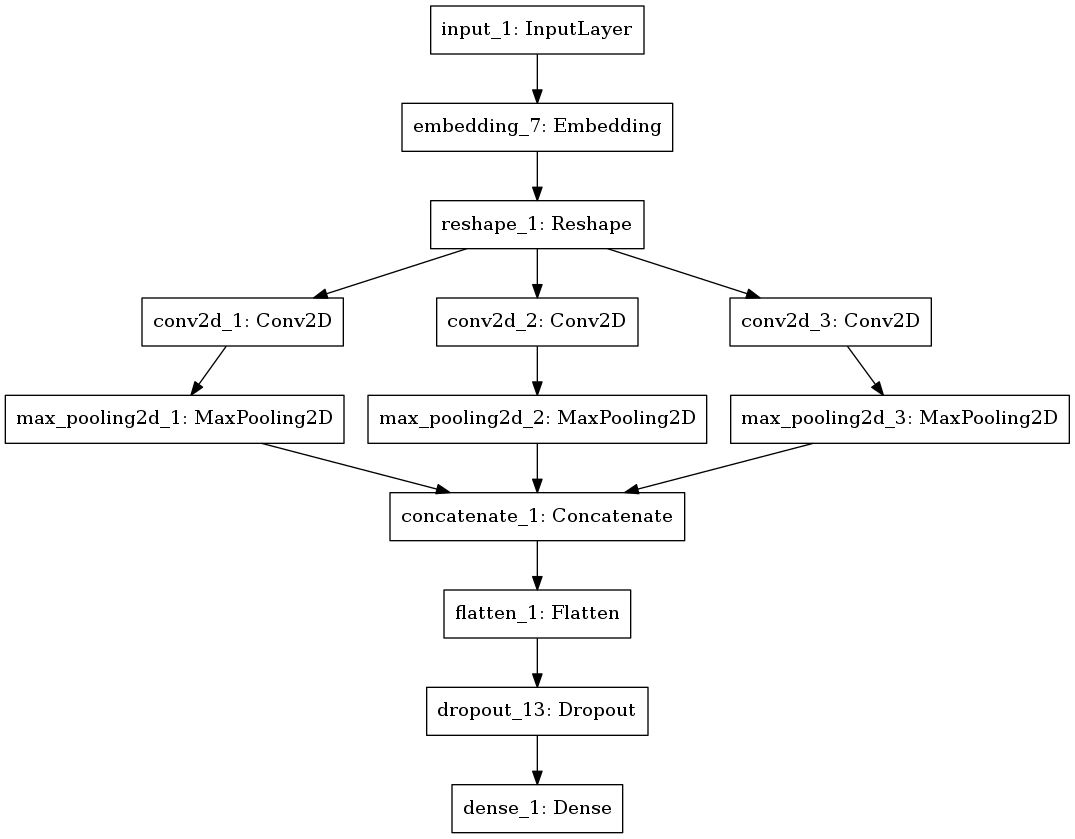
\includegraphics[width=0.7\textwidth]{images/super/arq_cnn}
	\caption{Arquitectura CNN}
	\label{fig:arqcnn}
\end{figure}


En la figura \ref{fig:arqcnn} podemos ver un ejemplo de un modelo de arquitectura de este tipo. Los modelos con la arquitectura que proponemos estarán formados por los siguientes tipos de capas: 

\begin{itemize}
\item \textbf{Entrada}: La entrada del modelo consistirá en una secuencia de identificadores de \textit{tokens}.

 \item \textbf{Embeddings}: Una vez tengamos la entrada se le aplicará un \textit{embedding}, en nuestro caso hemos realizado la mayoría de los modelos con \textit{Skip-gram}. Este modelo estará pre-entrenado y simplemente traducirá cada \textit{ID} de la secuencia de palabras en el vector de números reales a partir de la matriz entrenada con anterioridad. 
 
 \item \textbf{Capas convolucionales}: Este será el núcleo de este tipo de modelos y consistirán en un número $N$ de capas en las que se aplicarán distintos tipos de \textit{kernels} al conjunto de entrada.
 
 
 \item \textbf{Capas Pooling}: Se aplicará \textit{max-pooling} a la salida de cada una de las capas convolucionales. El objetivo es quedarnos con las características más relevantes de cada ``cuadrante''.
 
 
 \item \textbf{Capa de Dropout}: Tras concatenar y aplanar la salida introduciremos una capa de \textit{dropout} previa a la capa totalmente conectada. El objetivo de esta capa será evitar el sobreentrenamiento. 
 
   \item \textbf{Capa totalmente conectada}: Por último, una capa totalmente conectada nos dará la salida del modelo. En función de si nuestro objetivo es clasificación multiclase o binaria utilizaremos como salida la función \textit{softmax} o \textit{sigmoid} respectivamente.
 
 
 
\end{itemize}

Esta arquitectura podrá utilizarse para crear diferentes parámetros, en nuestro caso hemos jugado con los parámetros: 

\begin{itemize}
\item Número de capas convolucionales. 
\item Tamaño de los \textit{kernels} que se aplicarán en cada capa.
\item Número de \textit{kernels} que tendrá cada capa. 
\item Valor de \textit{dropout}.
\item Valor de regularización nivel dos. Este parámetro intentará reducir el sobreentrenamiento de la red, reduciendo los pesos altos. 
\end{itemize}



El código de creación y entrenamiento de un modelo de este tipo, usando el módulo \textit{mgmtfm} sería: 
\vspace{0.5cm}
   
   
    \begin{tcolorbox}[breakable, size=fbox, boxrule=1pt, pad at break*=1mm,colback=cellbackground, colframe=cellborder]
\begin{Verbatim}[commandchars=\\\{\}]
\PY{n}{models\PYZus{}steps} \PY{o}{=} \PY{n}{models}\PY{o}{.}\PY{n}{Models}\PY{p}{(}\PY{n}{n\PYZus{}classes}\PY{p}{,}\PY{n}{input\PYZus{}shape}\PY{p}{,}\PY{n}{embedding\PYZus{}dim}\PY{p}{,}
                             \PY{n}{vocabulary\PYZus{}size}\PY{p}{,}\PY{n}{embedding\PYZus{}matrix}\PY{p}{)}
\PY{n}{models\PYZus{}steps}\PY{o}{.}\PY{n}{model\PYZus{}cnn\PYZus{}1}\PY{p}{(}\PY{n}{n\PYZus{}classes}\PY{p}{,}\PY{n}{filter\PYZus{}sizes}\PY{o}{=}\PY{n}{filter\PYZus{}sizes}\PY{p}{,} \PY{n}{drop}\PY{o}{=}\PY{n}{dropout}\PY{p}{,} 
                              \PY{n}{num\PYZus{}filters}\PY{o}{=}\PY{n}{num\PYZus{}filters}\PY{p}{)}
\PY{n}{models\PYZus{}steps}\PY{o}{.}\PY{n}{compile\PYZus{}and\PYZus{}train}\PY{p}{(}\PY{n}{X\PYZus{}train}\PY{p}{,} \PY{n}{y\PYZus{}train}\PY{p}{,}\PY{n}{batch\PYZus{}size}\PY{o}{=}\PY{n}{batch}\PY{p}{,}
                              \PY{n}{epochs}\PY{o}{=}\PY{n}{epochs}\PY{p}{,} \PY{n}{lr}\PY{o}{=}\PY{n}{lr}\PY{p}{,}\PY{n}{decay}\PY{o}{=}\PY{n}{decay}\PY{p}{,} 
                              \PY{n}{validation\PYZus{}data}\PY{o}{=}\PY{p}{(}\PY{n}{X\PYZus{}test}\PY{p}{,} \PY{n}{y\PYZus{}test}\PY{p}{)}\PY{p}{,}
                              \PY{n}{loss}\PY{o}{=}\PY{n}{loss\PYZus{}function}\PY{p}{)} 
\end{Verbatim}
\end{tcolorbox}
   
   


\subsection{Red neuronal recurrente}
En este apartado vamos a crear una arquitectura basándonos en otro de los modelos que vimos al analizar el estado del arte, las redes neuronales recurrentes (apartado \ref{section:arte:arqu:cnn}). De nuevo usaremos los modelos entrenados con este tipo de arquitectura para clasificar llamadas.

Las redes recurrentes a simple vista pueden parecer la solución más intuitiva a la hora de abordar un problema de análisis/clasificación de textos con \textit{deep learning}. En este caso iremos pasando toda la secuencia de \textit{tokens}, proveniente de la transcripción de nuestras llamadas, y, en cada paso (o \textit{token}), la red irá olvidando características poco relevantes del mensaje y quedándose con las características importantes para su clasificación. Como podemos imaginar el entrenamiento de estas redes es un proceso más complejo y costoso computacionalmente que el de las redes convolucionales anteriormente vistas.




\begin{figure}[!ht]
	\centering
	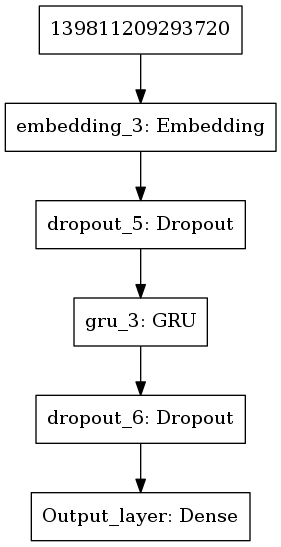
\includegraphics[width=0.25\textwidth]{images/super/arq_rnn1}
	\caption{Arquitectura RNN}
	\label{fig:arqrnn1}
\end{figure}


En la figura \ref{fig:arqrnn1} observamos un modelo de ejemplo con la arquitectura descrita. Los modelos con la arquitectura recurrente propuesta estarán formados por los siguientes tipos de capas: 

\begin{itemize}
\item \textbf{Entrada}: La entrada del modelo consistirá en una secuencia de identificadores de \textit{tokens}.

 \item \textbf{Embeddings}: Una vez tengamos la entrada, se le aplicará un \textit{embedding}, en nuestro caso hemos realizado la mayoría de los modelos con SKIP-Gram. Este modelo estará pre-entrenado y simplemente traducirá cada \textit{ID} de la secuencia de palabras en el vector de números reales a partir de la matriz entrenada con anterioridad. 
 
 
  \item \textbf{Capa de Dropout}:Posteriormente tendremos una capa de \textit{dropout} previa a la red recurrente. El objetivo de esta capa será evitar el sobreentrenamiento. Añadiremos otra capa de \textit{dropout} con el mismo objetivo previa a la capa totalmente conectada.
 
 \item \textbf{Capa recurrente}: En este punto introduciremos una capa formada por un número $N$ de celdas recurrentes. 
 
 
   \item \textbf{Capa totalmente conectada}: Por último, una capa totalmente conectada nos dará la salida del modelo. En función de si nuestro objetivo es clasificación multiclase o binaria, utilizaremos como salida la función \textit{softmax} o \textit{sigmoid} respectivamente.
 
\end{itemize}


Esta arquitectura podrá utilizarse para crear diferentes modelos, en nuestro caso hemos jugado con los parámetros: 

\begin{itemize}
\item Tipo de celda: LSTM o GRU. 
\item Número de celdas en la capa recurrente. 
\item Valor de \textit{dropout}.
\end{itemize}


El código de creación y entrenamiento de un modelo de este tipo, usando el módulo \textit{mgmtfm} sería: 
\vspace{0.5cm}
   
    \begin{tcolorbox}[breakable, size=fbox, boxrule=1pt, pad at break*=1mm,colback=cellbackground, colframe=cellborder]
\begin{Verbatim}[commandchars=\\\{\}]
\PY{n}{models\PYZus{}steps} \PY{o}{=} \PY{n}{models}\PY{o}{.}\PY{n}{Models}\PY{p}{(}\PY{n}{n\PYZus{}classes}\PY{p}{,}\PY{n}{input\PYZus{}shape}\PY{p}{,}\PY{n}{embedding\PYZus{}dim}\PY{p}{,}
                               \PY{n}{vocabulary\PYZus{}size}\PY{p}{,}\PY{n}{embedding\PYZus{}matrix}\PY{p}{)}
\PY{n}{models\PYZus{}steps}\PY{o}{.}\PY{n}{model\PYZus{}rnn\PYZus{}1}\PY{p}{(}\PY{n}{memory\PYZus{}units}\PY{p}{,} \PY{n}{cell\PYZus{}type}\PY{p}{,} \PY{n}{dropout}\PY{p}{)}
\PY{n}{models\PYZus{}steps}\PY{o}{.}\PY{n}{compile\PYZus{}and\PYZus{}train}\PY{p}{(}\PY{n}{X\PYZus{}train}\PY{p}{,} \PY{n}{y\PYZus{}train}\PY{p}{,}
                                \PY{n}{batch\PYZus{}size}\PY{o}{=}\PY{n}{batch}\PY{p}{,} \PY{n}{epochs}\PY{o}{=}\PY{n}{epochs}\PY{p}{,} 
                                \PY{n}{lr}\PY{o}{=}\PY{n}{lr}\PY{p}{,}\PY{n}{decay}\PY{o}{=}\PY{n}{decay}\PY{p}{,}
                                \PY{n}{validation\PYZus{}data}\PY{o}{=}\PY{p}{(}\PY{n}{X\PYZus{}test}\PY{p}{,} \PY{n}{y\PYZus{}test}\PY{p}{)}\PY{p}{,}
                                \PY{n}{loss}\PY{o}{=}\PY{n}{loss\PYZus{}function}\PY{p}{)} 
\end{Verbatim}
\end{tcolorbox}


\subsection{Red neuronal ``híbrida'' convolucional/recurrente}

Vistas las características de ambas redes pensamos en combinar ambas para obtener las bondades de cada una. Por un lado una capa convolucional que se encargara de recoger las características locales de la secuencia (extraer los ``N-Gramas'') y posteriormente, una capa recurrente que utilice la información enriquecida por la capa convolucional para realizar la clasificación.



\begin{figure}[!ht]
	\centering
	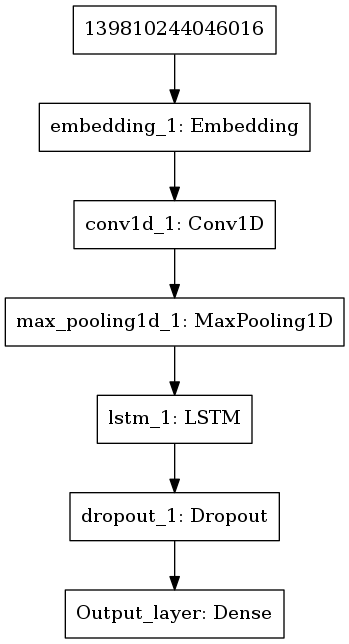
\includegraphics[width=0.25\textwidth]{images/super/arq_rnn2}
	\caption{Arquitectura ``Híbrida'' CNN/RNN}
	\label{fig:arqrnn2}
\end{figure}


En la figura \ref{fig:arqrnn2} podemos ver un ejemplo de un modelo de arquitectura de este tipo. Los modelos con la arquitectura que proponemos estarán formados por los siguientes tipos de capas:

 \begin{itemize}
 \item \textbf{Entrada}: La entrada del modelo consistirá en una secuencia de identificadores de \textit{tokens}.
 
  \item \textbf{Embeddings}: Una vez tengamos la entrada se le aplicará un \textit{embedding}, en nuestro caso hemos realizado la mayoría de los modelos con SKIP-Gram. Este modelo estará pre-entrenado y simplemente traducirá cada \textit{ID} de la secuencia de palabras en el vector de números reales a partir de la matriz entrenada con anterioridad. 
  
  \item \textbf{Capa convolucional}: En esta capa se aplicará un número determinado de \textit{kernels} con el tamaño especificado. 
  
 
  
  
  \item \textbf{Capa de Pooling}: Se aplicará \textit{max-pooling} a la salida de la capa convolucional. El objetivo es quedarnos con las características más relevantes de cada ``cuadrante''.
  
  
  \item \textbf{Capa de Dropout}: Tras la capa recurrente introduciremos una capa de \textit{dropout} previa a la capa totalmente conectada. El objetivo de esta capa será evitar el sobreentrenamiento. 
  
  
   \item \textbf{Capa recurrente}: En este punto introduciremos una capa formada por un número $N$ de celdas recurrentes. 
   
  
    \item \textbf{Capa totalmente conectada}: Por último, una capa totalmente conectada nos dará la salida del modelo. En función de si nuestro objetivo es clasificación multiclase o binaria utilizaremos como salida la función \textit{softmax} o \textit{sigmoid} respectivamente.
  
  
 \end{itemize}


Esta arquitectura podrá utilizarse para crear diferentes modelos, en nuestro caso hemos jugado con los parámetros: 


\begin{itemize}

\item Tipo de celda de la capa recurrente: LSTM o GRU. 
\item Número de celdas en la capa recurrente. 
\item Valor de \textit{dropout}.
\item Tamaño de los \textit{kernels} que se aplicarán en la capa convolucional. 
\item Número de \textit{kernels} que tendrá la capa convolucional. 
\item \textit{padding} (str): Tipo de padding a realizar al aplicar la capa convolucional..
\end{itemize}

El código de creación y entrenamiento de un modelo de este tipo, usando el módulo \textit{mgmtfm} sería: 

\vspace{0.5cm}

    
    \begin{tcolorbox}[breakable, size=fbox, boxrule=1pt, pad at break*=1mm,colback=cellbackground, colframe=cellborder]

\begin{Verbatim}[commandchars=\\\{\}]
\PY{n}{models\PYZus{}steps} \PY{o}{=} \PY{n}{models}\PY{o}{.}\PY{n}{Models}\PY{p}{(}\PY{n}{n\PYZus{}classes}\PY{p}{,}\PY{n}{input\PYZus{}shape}\PY{p}{,}\PY{n}{embedding\PYZus{}dim}\PY{p}{,}
                               \PY{n}{vocabulary\PYZus{}size}\PY{p}{,}\PY{n}{embedding\PYZus{}matrix}\PY{p}{)}
\PY{n}{models\PYZus{}steps}\PY{o}{.}\PY{n}{model\PYZus{}rnn\PYZus{}2}\PY{p}{(}\PY{n}{memory\PYZus{}units}\PY{p}{,} \PY{n}{cell\PYZus{}type}\PY{p}{,} \PY{n}{dropout}\PY{p}{,}
                               \PY{n}{filters}\PY{p}{,}\PY{n}{filter\PYZus{}size}\PY{p}{,}\PY{n}{pooling\PYZus{}size}\PY{p}{,} \PY{n}{padding}\PY{p}{)}
\PY{n}{models\PYZus{}steps}\PY{o}{.}\PY{n}{compile\PYZus{}and\PYZus{}train}\PY{p}{(}\PY{n}{X\PYZus{}train}\PY{p}{,} \PY{n}{y\PYZus{}train}\PY{p}{,}\PY{n}{batch\PYZus{}size}\PY{o}{=}\PY{n}{batch}\PY{p}{,} 
                               \PY{n}{epochs}\PY{o}{=}\PY{n}{epochs}\PY{p}{,} \PY{n}{lr}\PY{o}{=}\PY{n}{lr}\PY{p}{,}\PY{n}{decay}\PY{o}{=}\PY{n}{decay}\PY{p}{,} 
                               \PY{n}{validation\PYZus{}data}\PY{o}{=}\PY{p}{(}\PY{n}{X\PYZus{}test}\PY{p}{,} \PY{n}{y\PYZus{}test}\PY{p}{)}\PY{p}{,}
                               \PY{n}{loss}\PY{o}{=}\PY{n}{loss\PYZus{}function}\PY{p}{)} 
\end{Verbatim}
\end{tcolorbox}






\subsection{MLP}
Los modelos que hemos visto hasta hora tenían siempre como entrada una secuencia de palabras, sin embargo con la representación de palabras \textit{Doc2Vec} es posible obtener un vector con números reales para cada transcripción que contenga información semántica del mismo. Esto nos permite poder abordar otro tipo de modelos más simples.  

\begin{figure}[!ht]
	\centering
	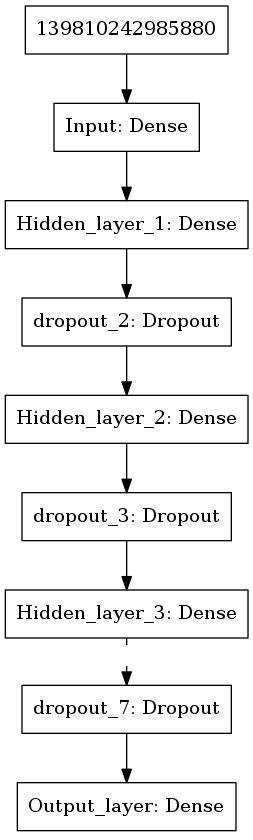
\includegraphics[width=0.20\textwidth]{images/super/arq_dense}
	\caption{Arquitectura con capas totalmente conectadas}
	\label{fig:arqdense}
\end{figure}

La arquitectura que proponemos, y que podemos ver en la figura \ref{fig:arqdense}, consiste en utilizar unicamente un número $N$ de capas totalmente conectadas y de \textit{dropout} (para evitar el sobreentrenamiento).

Los parámetros que podremos usar en este caso serían: 


\begin{itemize}

\item Número de capas totalmente conectadas. 
\item Número de neuronas en cada una de las capas. El número de neuronas de la última capa corresponderá con la salida y, en función de si nuestro objetivo es clasificación multiclase o binaria, utilizaremos como salida la función \textit{softmax} o \textit{sigmoid} respectivamente.
\item Valor de \textit{dropout}.
\end{itemize}


El código de creación y entrenamiento de un modelo de este tipo, usando el módulo \textit{mgmtfm} sería: 

\vspace{0.5cm}



    \begin{tcolorbox}[breakable, size=fbox, boxrule=1pt, pad at break*=1mm,colback=cellbackground, colframe=cellborder]
\begin{Verbatim}[commandchars=\\\{\}]
\PY{n}{models\PYZus{}steps} \PY{o}{=} \PY{n}{models}\PY{o}{.}\PY{n}{Models}\PY{p}{(}\PY{n}{n\PYZus{}classes}\PY{p}{,}\PY{n}{input\PYZus{}shape}\PY{p}{,}\PY{n}{embedding\PYZus{}dim}\PY{p}{,}
                               \PY{n}{vocabulary\PYZus{}size}\PY{p}{,}\PY{n}{embedding\PYZus{}matrix}\PY{p}{)}
\PY{n}{models\PYZus{}steps}\PY{o}{.}\PY{n}{model\PYZus{}dense\PYZus{}1}\PY{p}{(}\PY{n}{layers\PYZus{}list}\PY{p}{,}\PY{n}{drop}\PY{o}{=}\PY{n}{dropout}\PY{p}{)}
\PY{n}{models\PYZus{}steps}\PY{o}{.}\PY{n}{compile\PYZus{}and\PYZus{}train}\PY{p}{(}\PY{n}{X\PYZus{}train}\PY{p}{,} \PY{n}{y\PYZus{}train}\PY{p}{,}\PY{n}{batch\PYZus{}size}\PY{o}{=}\PY{n}{batch}\PY{p}{,} 
                               \PY{n}{epochs}\PY{o}{=}\PY{n}{epochs}\PY{p}{,} \PY{n}{lr}\PY{o}{=}\PY{n}{lr}\PY{p}{,}\PY{n}{decay}\PY{o}{=}\PY{n}{decay}\PY{p}{,} 
                               \PY{n}{validation\PYZus{}data}\PY{o}{=}\PY{p}{(}\PY{n}{X\PYZus{}test}\PY{p}{,} \PY{n}{y\PYZus{}test}\PY{p}{)}\PY{p}{,}
                               \PY{n}{loss}\PY{o}{=}\PY{n}{loss\PYZus{}function}\PY{p}{)} 
\end{Verbatim}
\end{tcolorbox}




\subsection{Combinación de modelos}
\label{section:super:mod:stack}

Otra opción que hemos abordado es la de combinar la salida de los modelos y que estos formen la entrada de un nuevo modelo de capas totalmente conectadas. 


\begin{figure}[!ht]
	\centering
	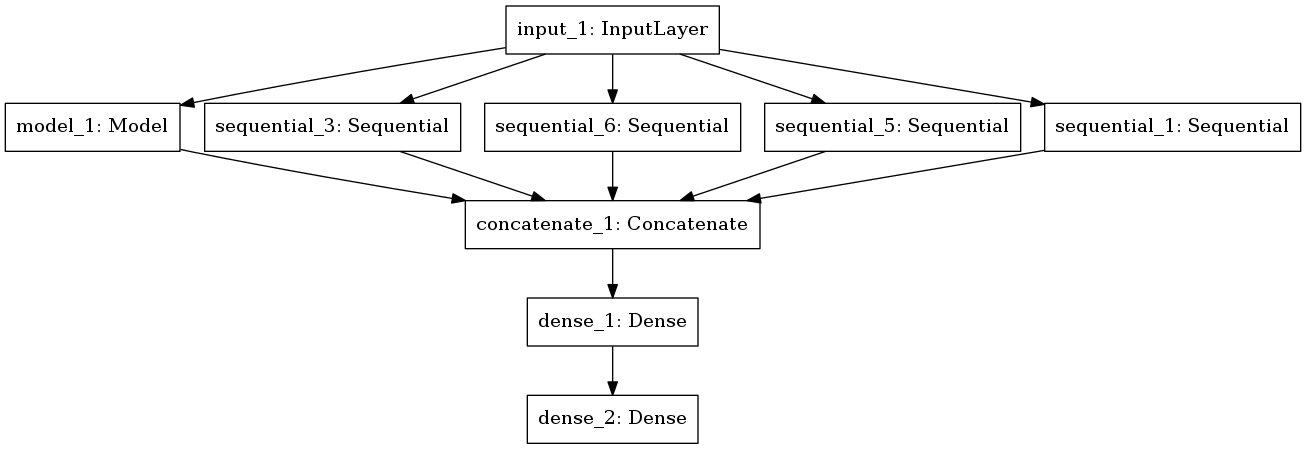
\includegraphics[width=1\textwidth]{images/super/arq_stack}
	\caption{Arquitectura con capas totalmente conectadas}
	\label{fig:arqstack}
\end{figure}


En la figura \ref{fig:arqstack}, vemos un ejemplo de este tipo de modelos. En este caso el input alimenta a los diferentes modelos (5 en este caso), que pueden estar construidos tanto con el modelo \textit{Model} de keras como con el modelo \textit{Sequential}.


La salida de los diferentes modelos se concatena y, antes de la salida, se añade una capa oculta totalmente conectada con función de activación \textit{relu}. Normalmente este tipo de modelos no vamos a usarlos para tareas de clasificación binaria, por lo que la función de activación de la capa de salida será \textit{sigmoid}.


Hay que destacar que los sub-modelos que forman parte de este modelo están preentrenados y no volverán a entrenarse en el proceso de aprendizaje.


En este caso no tenemos implementado el modelo en el módulo \textit{mgmtfm}, pero podemos basarnos en una lista de modelos creados en \textit{mgmtfm} ``$prev\_models$'' para crearlo: 
\vspace{0.5cm}

    \begin{tcolorbox}[breakable, size=fbox, boxrule=1pt, pad at break*=1mm,colback=cellbackground, colframe=cellborder]
\begin{Verbatim}[commandchars=\\\{\}]
\PY{k+kn}{from} \PY{n+nn}{keras}\PY{n+nn}{.}\PY{n+nn}{layers} \PY{k}{import} \PY{n}{Input}\PY{p}{,} \PY{n}{Dense}\PY{p}{,}  \PY{n}{concatenate}
\PY{k+kn}{from} \PY{n+nn}{keras}\PY{n+nn}{.}\PY{n+nn}{models} \PY{k}{import} \PY{n}{Model}

\PY{k}{for} \PY{n}{pm} \PY{o+ow}{in} \PY{n}{prev\PYZus{}models}\PY{p}{:}
    \PY{k}{for} \PY{n}{layer} \PY{o+ow}{in} \PY{n}{pm}\PY{o}{.}\PY{n}{\PYZus{}model}\PY{o}{.}\PY{n}{layers}\PY{p}{:}
        \PY{n}{layer}\PY{o}{.}\PY{n}{trainable} \PY{o}{=} \PY{k+kc}{False}


\PY{n}{models\PYZus{}out} \PY{o}{=} \PY{p}{[}\PY{n}{pm}\PY{o}{.}\PY{n}{\PYZus{}model}\PY{p}{(}\PY{n}{in\PYZus{}model}\PY{p}{)} \PY{k}{for} \PY{n}{pm} \PY{o+ow}{in} \PY{n}{prev\PYZus{}models}\PY{p}{]}
\PY{n}{combined} \PY{o}{=} \PY{n}{concatenate}\PY{p}{(}\PY{n}{models\PYZus{}out}\PY{p}{)}
\PY{n}{hidden} \PY{o}{=} \PY{n}{Dense}\PY{p}{(}\PY{n}{n\PYZus{}hidden}\PY{p}{,} \PY{n}{activation}\PY{o}{=}\PY{l+s+s1}{\PYZsq{}}\PY{l+s+s1}{relu}\PY{l+s+s1}{\PYZsq{}}\PY{p}{)}\PY{p}{(}\PY{n}{combined}\PY{p}{)}
\PY{n}{out\PYZus{}model} \PY{o}{=} \PY{n}{Dense}\PY{p}{(}\PY{n}{n\PYZus{}classes}\PY{p}{,} \PY{n}{activation}\PY{o}{=}\PY{l+s+s1}{\PYZsq{}}\PY{l+s+s1}{softmax}\PY{l+s+s1}{\PYZsq{}}\PY{p}{)}\PY{p}{(}\PY{n}{hidden}\PY{p}{)}
\PY{n}{model} \PY{o}{=} \PY{n}{Model}\PY{p}{(}\PY{n}{in\PYZus{}model} \PY{p}{,} \PY{n}{out\PYZus{}model}\PY{p}{)}
\end{Verbatim}
\end{tcolorbox}

Y posteriormente entrenarlo: 

\vspace{0.5cm}

    \begin{tcolorbox}[breakable, size=fbox, boxrule=1pt, pad at break*=1mm,colback=cellbackground, colframe=cellborder]
\begin{Verbatim}[commandchars=\\\{\}]
\PY{k+kn}{from} \PY{n+nn}{keras}\PY{n+nn}{.}\PY{n+nn}{optimizers} \PY{k}{import} \PY{n}{Adam}
\PY{k+kn}{from} \PY{n+nn}{keras}\PY{n+nn}{.}\PY{n+nn}{preprocessing}\PY{n+nn}{.}\PY{n+nn}{sequence} \PY{k}{import} \PY{n}{pad\PYZus{}sequences}

\PY{n}{adam} \PY{o}{=} \PY{n}{Adam}\PY{p}{(}\PY{n}{lr}\PY{p}{,} \PY{n}{decay}\PY{o}{=}\PY{n}{decay}\PY{p}{)}
        
\PY{n}{model}\PY{o}{.}\PY{n}{compile}\PY{p}{(}\PY{n}{loss}\PY{o}{=}\PY{n}{loss}\PY{p}{,}
                    \PY{n}{optimizer}\PY{o}{=}\PY{n}{adam}\PY{p}{,}
                    \PY{n}{metrics}\PY{o}{=}\PY{n}{metrics}  \PY{p}{)}

\PY{n}{model}\PY{o}{.}\PY{n}{fit}\PY{p}{(}\PY{n}{X\PYZus{}train}\PY{p}{,} \PY{n}{y\PYZus{}train}\PY{p}{,} \PY{n}{batch\PYZus{}size}\PY{o}{=}\PY{n}{batch\_size}\PY{p}{,} \PY{n}{epochs}\PY{o}{=}\PY{n}{epochs}\PY{p}{,}
                        \PY{n}{validation\PYZus{}data}\PY{o}{=}\PY{p}{(}\PY{n}{X\PYZus{}test} \PY{p}{,} \PY{n}{y\PYZus{}test}\PY{p}{)}\PY{p}{)} 
\end{Verbatim}
\end{tcolorbox}



\section{Evaluación y optimización}
\label{section:super:opt}
Una vez hemos creado los modelos acordes a las diferentes arquitecturas comentadas en el apartado anterior, surge la necesidad de encontrar los hiperparámetros que en cada arquitectura nos lleven a la mayor precisión de nuestro modelo.


Encontrar los mejores parámetros es una tarea crucial a la hora de probar un modelo y ,aunque existen diferentes métodos para intentar conseguir los mejores resultados al entrenar nuestro modelo, como puede ser definir un \textit{grid} de parámetros o probar de manera aleatoria; nosotros hemos probado por un mecanismo más automático utilizando \textbf{Optuna}.

Optuna es un \textit{framework} de optimización de modelos que utiliza métodos Bayesianos para la optimización de modelos.  Entre las ventajas de Optuna tenemos: 

\begin{itemize}
\item Utilización de una BBDD (en nuestro caso PostgreSQL) que nos permite continuar con los entrenamientos cuando queramos y lanzar varios entrenamientos en paralelo o en cualquier momento. 
\item Posibilidad de definir la duración de las pruebas que queremos lanzar. Lo que nos permite, por ejemplo, lanzar pruebas por la noche cuando el clúster posee más recursos.  

\item Uso de la poda para descartar modelos con mala calidad en fases tempranas, ahorrando tiempo de cómputo. 
\end{itemize}


\textit{Optuna} necesita como parámetro una función a optimizar, en nuestro caso hemos decidido utilizar el \textit{accuracy} sobre el conjunto de \textit{test}. Este conjunto de \textit{test} estará formado por un tercio de los datos, mientras que los dos tercios restantes se dedicarán al conjunto de \textit{train}.


Desde que empezamos a usar \textit{Optuna} en la plataforma formada por \textit{GPUs} $Tesla V100-SXM2 32GB$, hemos dedicado unas 340 horas a la optimización de modelos, lo que supone algo más de 14 días. Hay que tener en cuenta que muchas de las pruebas no prometedoras \textit{Optuna} las ha cancelado automáticamente, por lo que en condiciones normales hubiéramos necesitado bastante más tiempo. También hay momentos en los que se ha paralelizado el entrenamiento entre varias \textit{GPUs}.


A lo largo del apartado veremos las distintas pruebas realizadas agrupándolas por tipo de arquitectura. Los nombres de los modelos nos darán
información sobre el tipo del modelo. Algunos datos que tenemos que
tener en cuenta son:
\begin{itemize}
 

\item \textbf{\textit{CNN/RNN/RNN2/DENSE}}: Nos indica el tipo del modelo y estará al comienzo
del nombre.

\item \textbf{\textit{IVR/MONI}}: Nos indica si el modelo ha sido entrenado y validado con los
tipos de IVR o de monitorizaciones. De momento solo usamos \textit{IVR} debido al porcentaje tan bajo de llamadas que poseen monitorizaciones.

\item \textbf{\textit{W2V150QC}}: Nos indica que utiliza un \textit{Word2Vec} con una dimensión de 150 y
quitando las palabras comunes en los \textit{tokens}.

\item \textbf{\textit{BIN/MULTI}}: Nos indica que se trata de un modelo binario o multiclase. Si
es binario al final del nombre nos encontramos la clase, si es multiclase y
no clasifica todas las clases nos encontramos las iniciales de las
clases.

\item \textbf{\textit{QX}}: Nos indica las clases que se eliminan. Por ejemplo \textit{QR\_QN} elimina
las clases \textit{resto} y \textit{no reconocido} antes de entrenar. La \textit{no reconocido} la
eliminamos siempre ya que puede contener elementos del resto de clases.

\item \textbf{\textit{866}}: Indica que en estos modelos se ha limitado las secuencias a 866
tokens, que engloban más del 99\% de las llamadas.

 \end{itemize}

Una última consideración a tener en cuenta es que, solo los modelos más prometedores se han pasado a la fase de optimización con \textit{Optuna}. Otros tantos, como pueden ser los modelos con datos de monitorizaciones, se han descartado desde un primer momento observando que los primeros resultados no eran prometedores.

\subsection{Modelos \textit{CNN} binarios}
Aunque se han hecho pruebas con modelos multi-clase, cuando se ha
empezado a utilizar \textit{Optuna} unicamente se han entrenado modelos binarios
que presentaban mucho mejores resultados. Por ello en esta primera sesión únicamente presentaremos datos de modelos convolucionales. 

Para cada modelo mostraremos los siguientes campos: 

\begin{itemize}
\item \textbf{\textit{study}}: Nombre del modelo del que se está realizando el estudio. 
\item \textbf{\textit{accuracy}}: Mejor precisión sobre el conjunto de test.
 \item \textbf{\textit{params}}: Parámetros con los que se ha obtenido la mejor precisión. 
  \item \textbf{\textit{ntrials}}: Número de pruebas realizadas del estudio. Cuenta las pruebas podadas, pero no las fallidas. 
    \item \textbf{\textit{total\_time}}: Tiempo total invertido en el entrenamiento del modelo.
    \item \textbf{\textit{best\_trial}}: Identificador de la mejor prueba realizada. Nos será de utilidad ya que \textit{Optuna} guarda los pesos automáticamente del mejor modelo.
\end{itemize}


\begin{figure}[!ht]
	\centering
	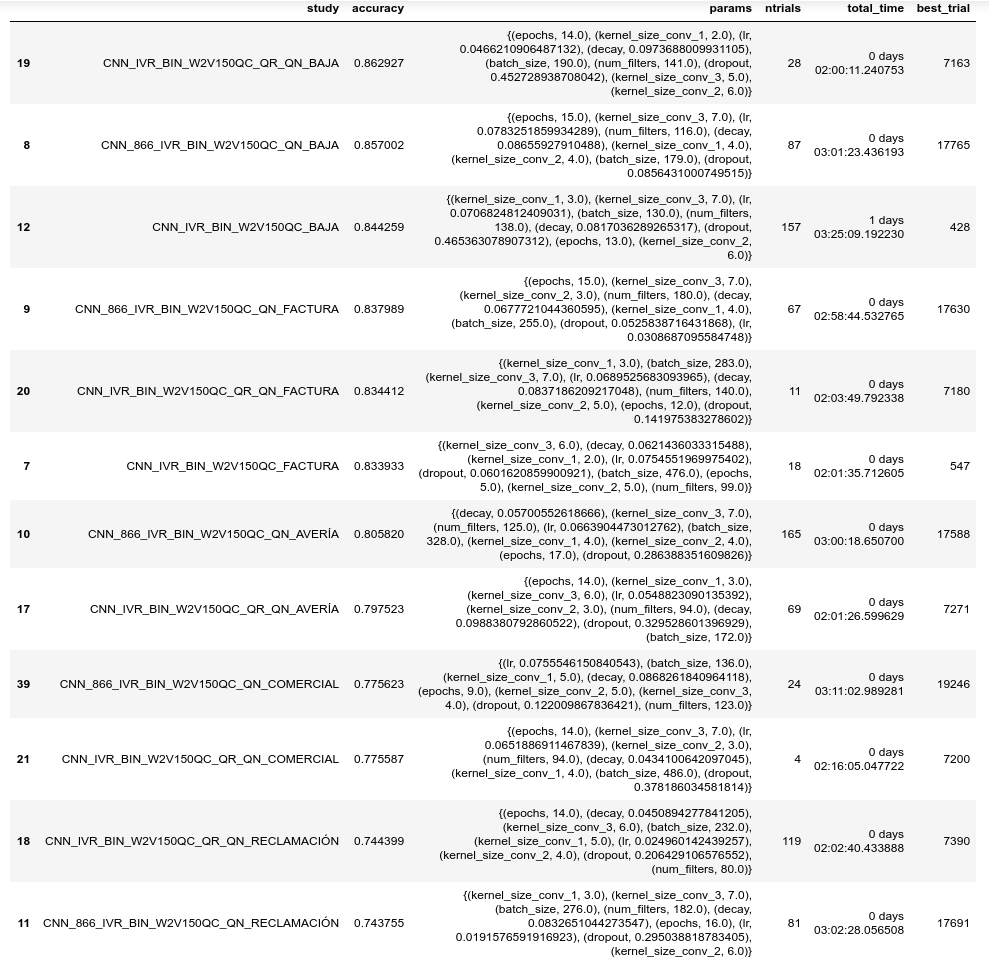
\includegraphics[width=1\textwidth]{images/super/opt_cnn}
	\caption{Optimización de modelos binarios con redes convolucionales}
	\label{fig:opt_cnn}
\end{figure}

  Los modelos se han entrenado
 con datos balanceados, teniendo el mismo número de muestras de la clase binaria y del resto de
clases. 


En la figura \ref{fig:opt_cnn} podemos ver los resultados obtenidos. Los resultados parecen bastante buenos para la mayoría de clases que van desde el 72\% al 86\% de precisión. Cuando eliminamos las clases \textit{resto} y \textit{no reconocido} vemos que los datos mejoran. Esto se debe a que, probablemente, existan datos en estas clases que hagan referencia a elementos de otras clases.


\subsection{Modelos \textit{RNN} Binarios}

A continuación presentamos los resultados de los modelos formados por redes recurrentes que realizan clasificación binaria en el mismo formato que el apartado anterior. Hemos agrupado en los modelos recurrentes también aquellos que tienen una capa convolucional junto a la capa recurrente. 

\begin{figure}[!ht]
	\centering
	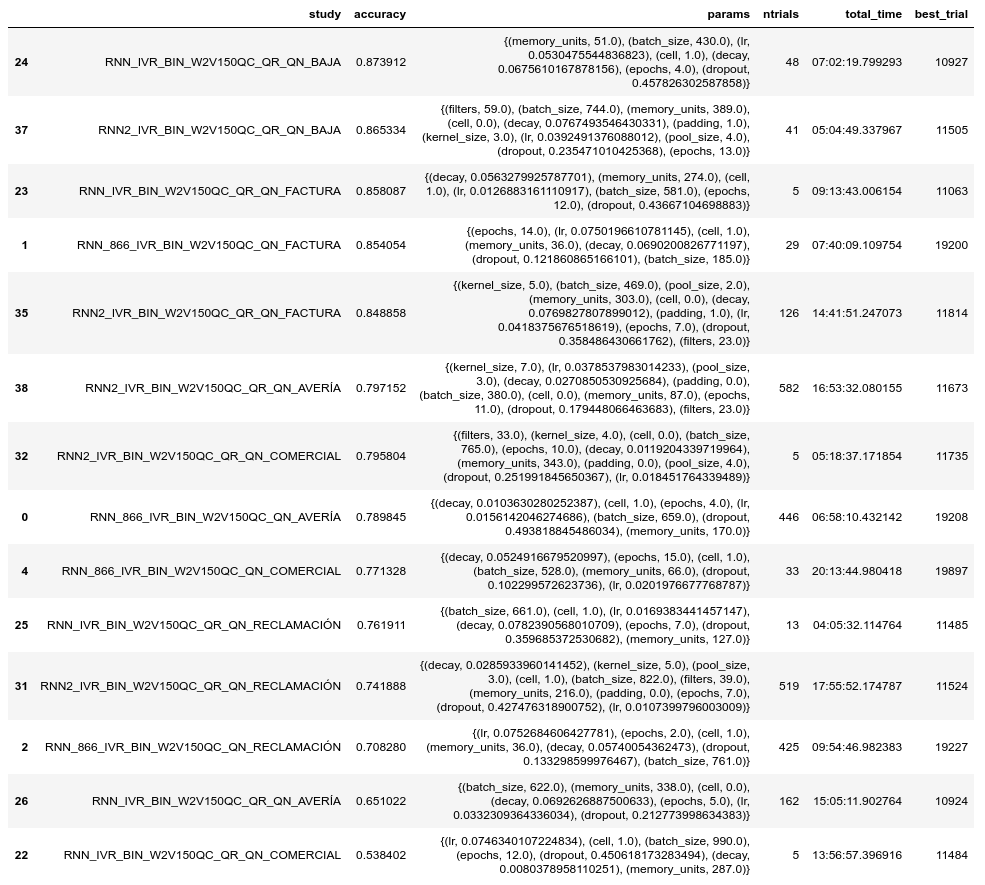
\includegraphics[width=1\textwidth]{images/super/opt_rnn_bin}
	\caption{Optimización de modelos binarios con redes recurrentes}
	\label{fig:opt_rnn}
\end{figure}


En general, observando la figura \ref{fig:opt_rnn}, vemos una ligera mejora con respecto a los modelos formados por redes convolucionales. Vemos por ejemplo como en el caso de la clase \textit{Factura} hemos mejorado el modelo hasta casi el 86\% con una red recurrente y el caso de la clase \textit{Comercial} con una red recurrente con una capa convolucional hemos llegado al 79.6\%. 

También podemos observar que no existe una diferencia apreciable entre los modelos que incluyen una capa convolucional y los que no la tienen. Otro punto a destacar de estas pruebas es que el tiempo de ejecución medio, si observamos el tiempo total y el número de pruebas, es mucho mayor que en los modelos convolucionales. 

En cuanto al tipo de celdas vemos que aunque aparecen ambos (valor 0 para $LSTM$ y valor 1 para $GRU$) los mejores resultados los hemos obtenido con $GRU$ siendo además los modelos con este tipo de celdas menos costosos para el entrenamiento. 

\subsection{Modelos totalmente conectados}

A continuación presentamos algunas pruebas, también de clasificación binaria, que realizamos utilizando como entrada directamente los vectores \textit{Doc2Vec} de las transcripciones.  

\begin{figure}[!ht]
	\centering
	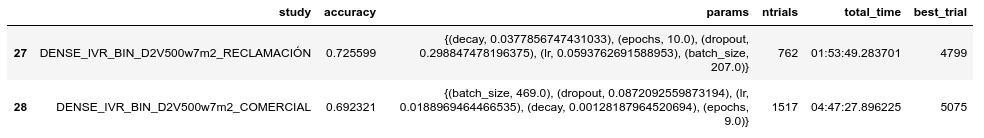
\includegraphics[width=1\textwidth]{images/super/opt_dense}
	\caption{Optimización de modelos binarios con \textit{MLP}}
	\label{fig:opt_dense}
\end{figure}

Como observamos en la figura \ref{fig:opt_dense}, unicamente hemos realizado pruebas de optimización con las clases \textit{Reclamación} y \textit{Comercial} devolviendo unos resultados de precisión sobre el conjunto de test del 72\% y 69\% respectivamente. El hecho de que los modelos anteriormente presentados tuvieran una mayor precisión nos llevó a no continuar por esta vía. 
 

\subsection{Modelos multiclase}

Hasta ahora todos los modelos que hemos presentado son binarios y hemos tenido resultados bastante aceptables en estos casos. En este apartado vamos a mostrar modelos multiclase basados en las mismas arquitecturas vistas anteriormente.



\begin{figure}[!ht]
	\centering
	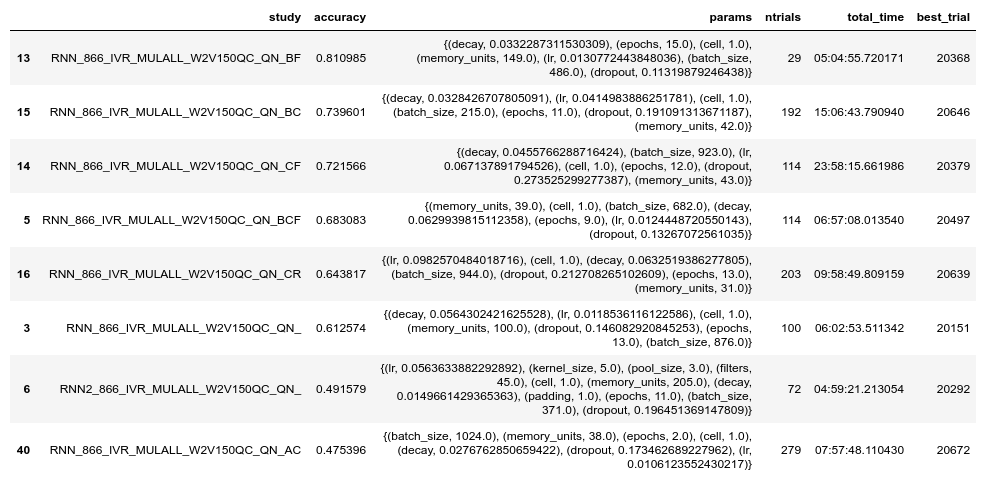
\includegraphics[width=1\textwidth]{images/super/opt_multi}
	\caption{Optimización de modelos multiclase}
	\label{fig:opt_multi}
\end{figure}

En la figura \ref{fig:opt_multi} podemos observar  los modelos multiclase que hemos construido y optimizado. Vemos que todos ellos los hemos construido con redes recurrentes de distintos tipos, que son las que, hasta ahora, nos han dado mejores resultados.  Aunque hicimos también  varias pruebas de conectar varios modelos binarios con la arquitectura propuesta en \ref{section:super:mod:stack} los resultados no fueron satisfactorios y la calidad disminuía considerablemente. 


Las últimas iniciales del campo \textit{study} nos indican las clases que el modelo es capaz de distinguir, si acaba en ``\_'' el modelo clasifica entre todas las clases.

Vemos que la mejor precisión en un modelo multiclase la tenemos hasta el momento en un modelo con redes recurrentes que distingue entrelas clases \textit{baja}, \textit{facturas} y el resto de llamadas con una precisión del 81\%.



\section{Resumen de modelos}
\label{section:super:resumen}

Tras la gran cantidad de modelos supervisados entrenados y vistos a lo largo de este capítulo, el objetivo de esta sección es hacer un breve resumen en el que poder acceder de un vistazo y de una manera más visual a todos ellos. 


\begin{figure}[!ht]
	\centering
	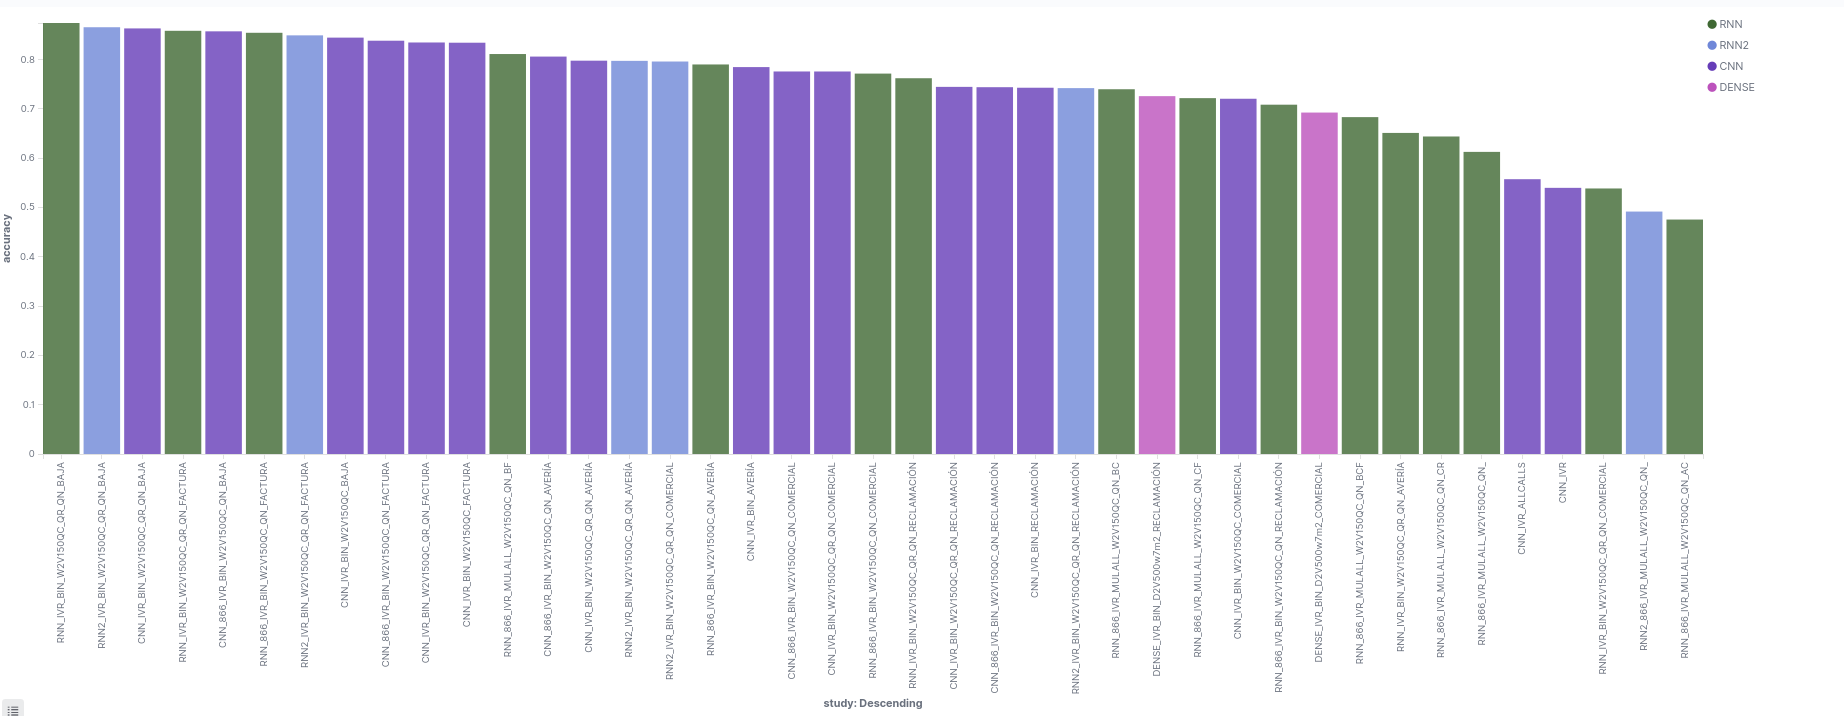
\includegraphics[width=1\textwidth]{images/super/resumen_todos}
	\caption{Precisión de todos los modelos}
	\label{fig:resumen_todos}
\end{figure}

En la figura \ref{fig:resumen_todos} podemos ver todos los modelos ordenados por precisión y coloreados según el tipo de arquitectura usada. Observamos que los modelos con más precisión se tratan de modelos con las arquitecturas recurrentes, convolucional e híbrida vistas en la sección \ref{section:super:arq}.



\begin{figure}[!ht]
	\centering
	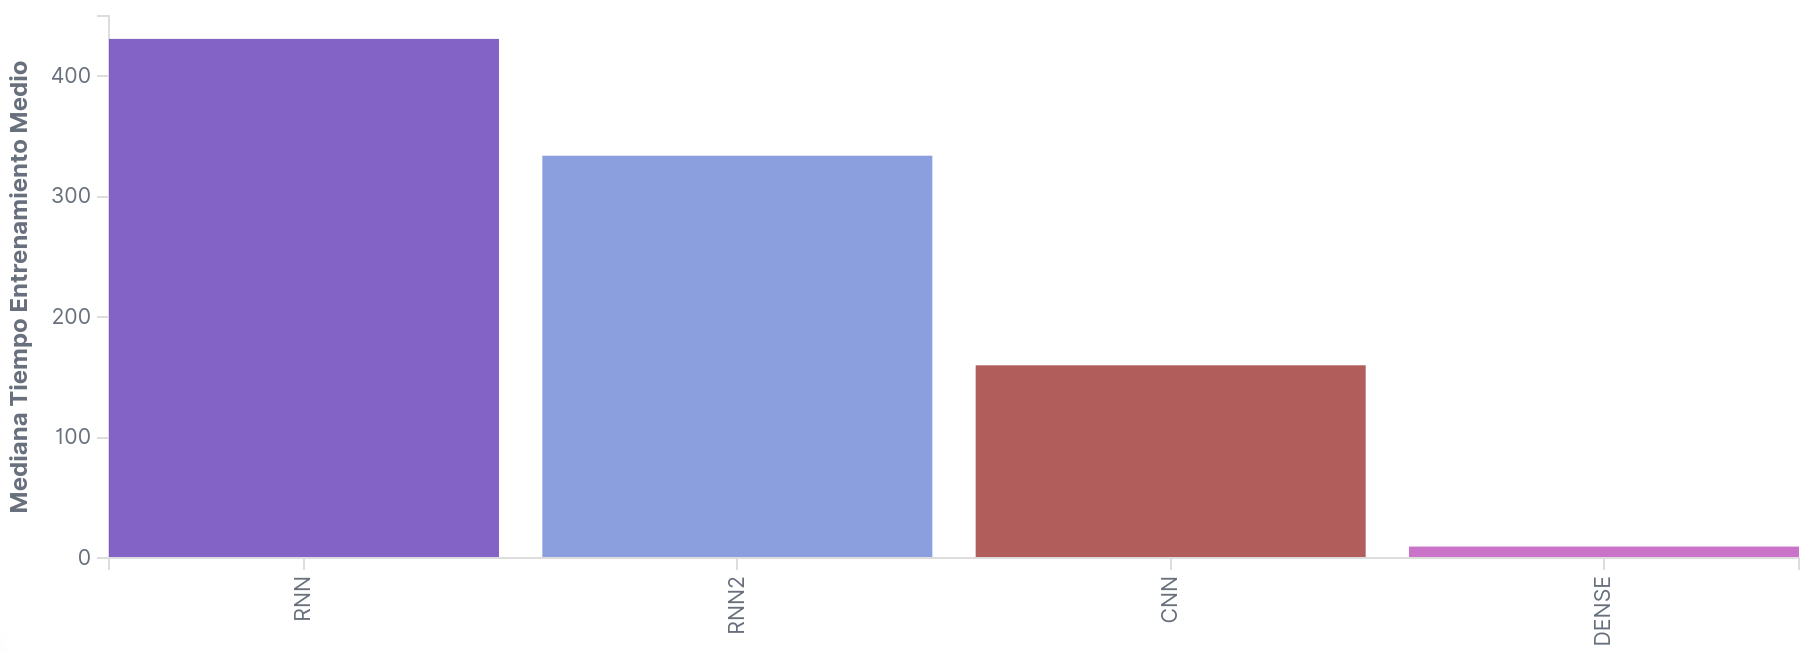
\includegraphics[width=1\textwidth]{images/super/resumen_tiempo}
	\caption{Mediana de ejecución de las diferentes arquitecturas}
	\label{fig:resumen_tiempo}
\end{figure}

Otro dato interesante es el tiempo de ejecución que requiere cada arquitectura. En la figura \ref{fig:resumen_tiempo} podemos ver la mediana de ejecución de todos los modelos, que nos servirá para hacernos una idea de la diferencia entre arquitecturas. Vemos que las arquitecturas con redes recurrentes son las más costosas de entrenar, mientras que las totalmente conectadas son las que menos tiempo han supuesto. En el cuadro \ref{tbl:resumen_tiempo} podemos observar el detalle sobre el tiempo de ejecución en formato tabular.

\begin{table} 
\label{tbl:resumen_tiempo}
\centering
\begin{tabular}{|c|c|}
\hline 
\textbf{Modelo} &\textbf{ Mediana Tiempo Medio (mm:ss)} \\ 
\hline 
 Recurrente &   07:11 \\ 
\hline 
Recurrente Híbrido &  05:34 \\ 
\hline 
 Convolucional &  02:30 \\ 
\hline 
 Totalmente Conectado &  00:10\\ 
\hline 
\end{tabular}
\caption{Mediana de ejecución de las diferentes arquitecturas} 
\end{table}

Dada la gran cantidad de modelos existentes vamos a hacer un primer filtro dependiendo de si estamos tratando la clasificación como binario o multiclase.

 
\subsection{Modelos binarios}


\begin{figure}[!ht]
	\centering
	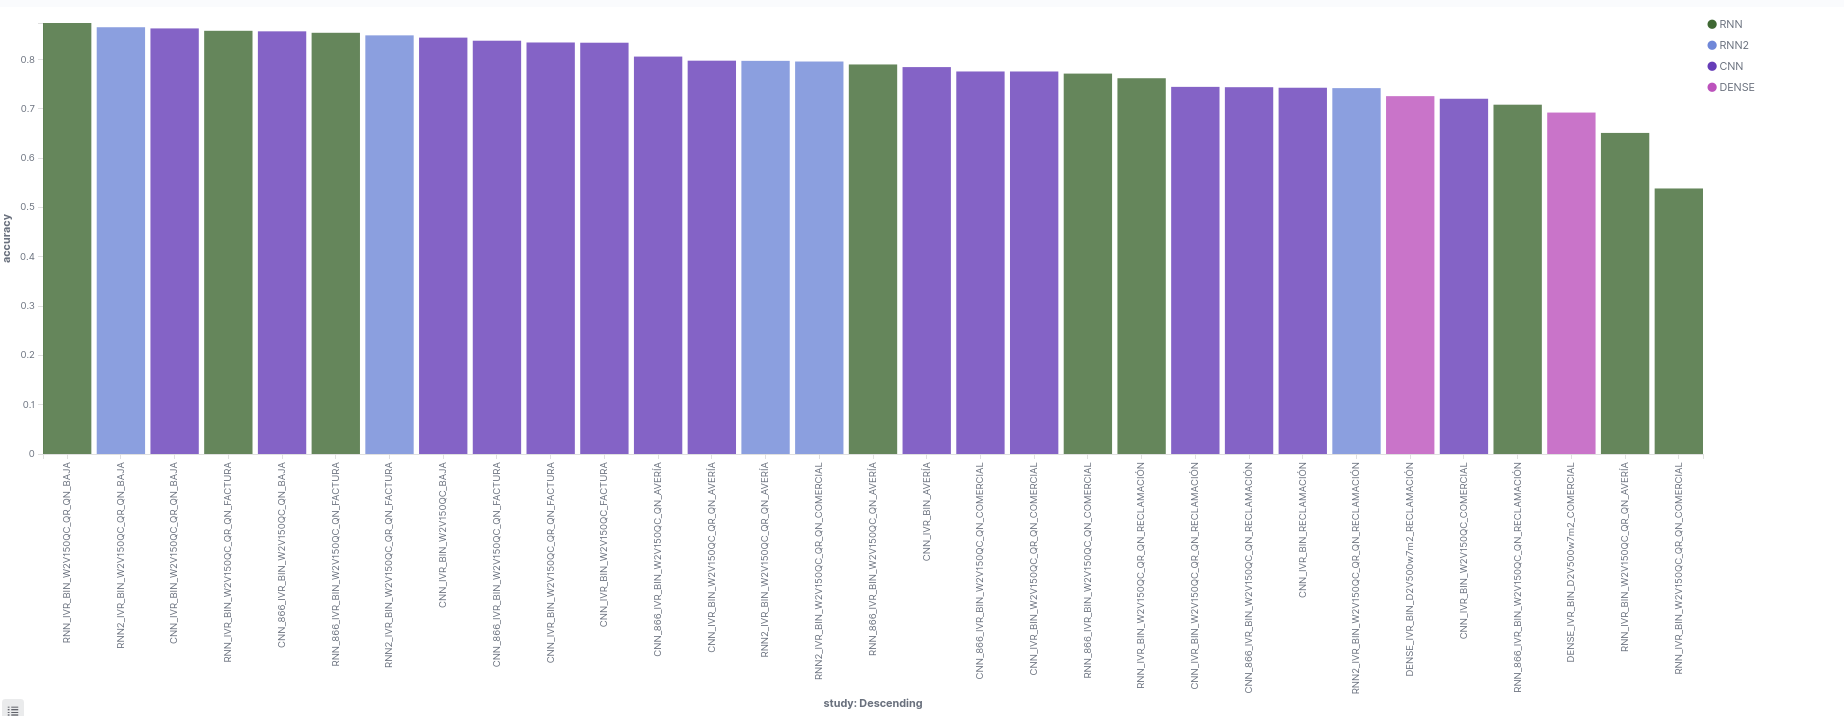
\includegraphics[width=1\textwidth]{images/super/resumen_bin}
	\caption{Precisión de los modelos binarios}
	\label{fig:resumen_bin}
\end{figure}

En la figura \ref{fig:resumen_bin}, vemos todos los modelos binarios entrenados y la precisión de cada uno. Como podemos observar los modelos binarios son la mayoría de los creados, por lo que la visión no cambia mucho con respecto a la figura \ref{fig:resumen_todos}.

\begin{figure}[!ht]
	\centering
	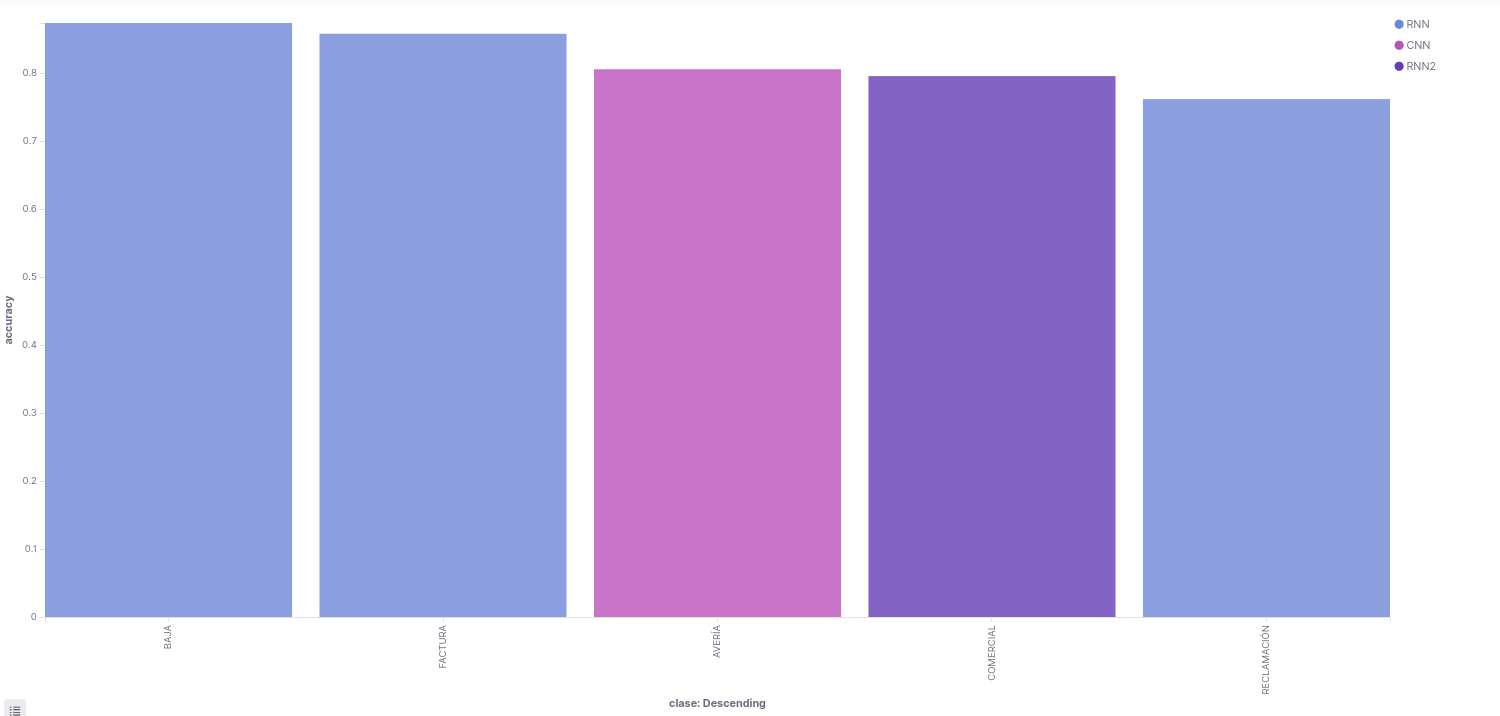
\includegraphics[width=1\textwidth]{images/super/resumen_bestbin}
	\caption{Precisión por clase de modelos binarios}
	\label{fig:resumen_bestbin}
\end{figure}

Para tener una visión más clara de la bondad de los modelos binarios, vamos a mostrar la precisión del mejor modelo entrenado para cada una de las clases y su arquitectura. Como podemos observar en la figura \ref{fig:resumen_bestbin} la arquitectura que mejor resultado nos ha dado es la arquitectura con redes recurrentes, aunque también se cuela un modelo convolucional y uno híbrido. En todos los casos la precisión está en torno al 80\%.

\subsection{Modelos multiclase}

Aunque hay algunos modelos multiclase realizados con otras arquitecturas, los únicos con un rendimiento aceptable se encuentran implementados con la arquitectura de redes recurrentes.

\begin{figure}[!ht]
	\centering
	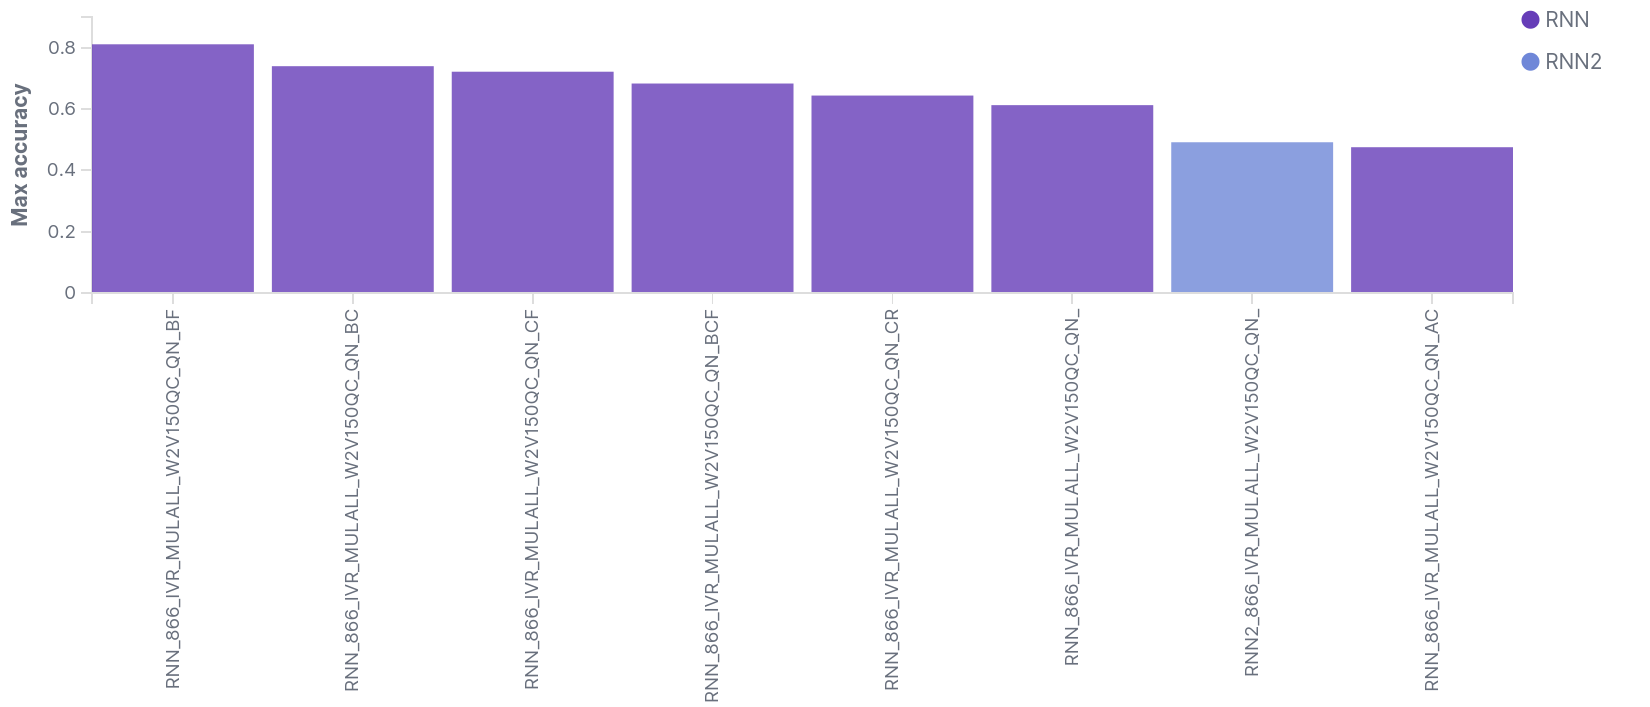
\includegraphics[width=1\textwidth]{images/super/resumen_multi}
	\caption{Precisión de los modelos multiclase}
	\label{fig:resumen_multi}
\end{figure}


En la figura \ref{fig:resumen_multi}  podemos ver los diferentes modelos multiclase entrenados, junto con su precisión en el conjunto de test. Observamos que el único modelo que posee un rendimiento superior al 80\% es el modelo que nos permite clasificar las clases \textit{Baja} y \textit{Factura}.


\section{Modelo Mínimo Viable}
\label{section:super:mvm}
El título de este apartado esta basado en el concepto de mínimo producto viable (MVP por sus siglas en inglés) acuñado por la metodología \textit{Lean Startup}. Un producto mínimo viable debe reunir las características mínimas para satisfacer a los primeros clientes y poder crear una retroalimentación que ayude a que sea mejorado en el futuro. En nuestro caso queremos llevar a producción uno de los modelos diseñados hasta ahora para poder construir un sistema completo y obtener \textit{feedback} que nos ayude en futuras mejoras.

El modelo que hemos seleccionado es el mejor modelo del estudio ``RNN\_866\_IVR\_MULALL\_W2V150QC\_QN\_BF'' y podemos verlo en las figura \ref{fig:opt_multi} y \ref{fig:resumen_multi}. Se trata de un modelo basado en la arquitectura de redes recurrentes, con 149 celdas tipo $GRU$ y que toma como entrada una secuencia de 866 \textit{Tokens} (El 99\% de las transcripciones están por debajo de este número de \textit{tokens}).


\begin{figure}[!ht]
	\centering
	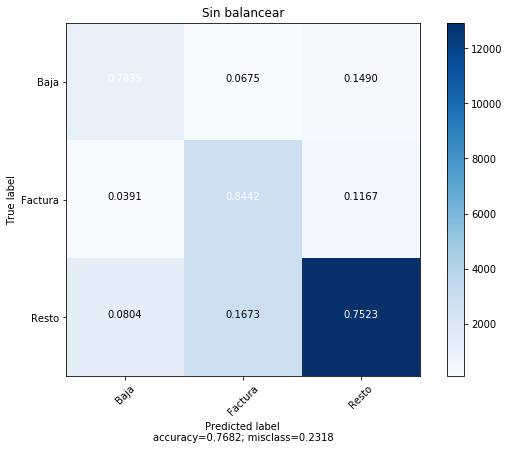
\includegraphics[width=0.65\textwidth]{images/super/mvp_mat1}
	\caption{Matriz de confusión datos balanceados}
	\label{fig:mvp_mat1}
\end{figure}


A continuación vamos a volver a medir la precisión del modelo usando tanto datos balanceados como sin balancear con el objetivo de verificar que el modelo pueda ser usado en un entorno productivo.




\begin{figure}[!ht]
	\centering
	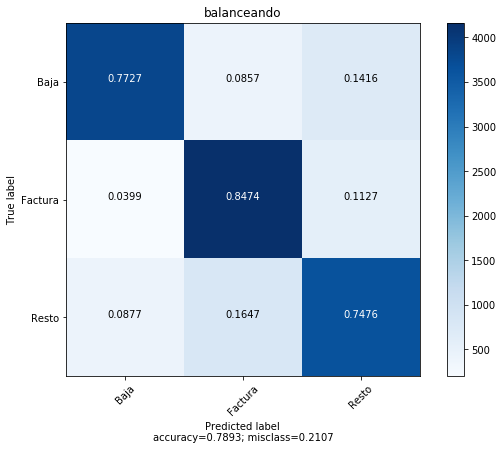
\includegraphics[width=0.65\textwidth]{images/super/mvp_mat2}
	\caption{Matriz de confusión datos no balanceados}
	\label{fig:mvp_mat2}
\end{figure}

En la figura \ref{fig:mvp_mat1} podemos ver la precisión del modelo con datos balanceados, mientras que en la figura  \ref{fig:mvp_mat2} vemos estos mismos datos sin balancear. Observamos que en el modelo sin balancear la mayoría de muestras se concentran en el resto, lo que es normal, ya que hay más llamadas de otros tipos que de \textit{Baja} y \textit{Factura}. Sin embargo, podemos ver que la precisión no varía sustancialmente por lo que el modelo es susceptible de usar en producción.


La siguiente parte del documento tratará de llevar a producción este modelo para que sea capaz de clasificar las llamadas en tiempo real con todo lo que ello implica. A partir de ahora nos referiremos a el como el modelo \textit{\textbf{bajafactura}} y lo veremos como una caja negra en la que solo nos preocuparemos por la forma en la que debemos introducir los datos y por las clasificaciones devueltas por el mismo.








\part{Explotación: procesamiento, visualización y alarmados}
\chapter{Capa de \textit{streaming}}
\label{chapter:prod}

En los anteriores capítulos hemos descrito el proceso completo que hemos realizado con los datos: Los hemos localizado, los hemos limpiado, hemos creado diferentes modelos de minería de datos y hemos repetido estos pasos de manera iterativa. En este capítulo comentaremos el camino seguido para llevar los modelos construidos a un entorno productivo real.

Este paso que relata el viaje ``del laboratorio a la fábrica'', nos permitirá  cumplir el segundo objetivo planteado en la sección \ref{section:intro:objetivos} del documento: \textbf{extraer esta temática para nuevas llamadas en tiempo real}. Además como veremos en la sección \ref{section:prod:req} será necesaria para cumplir con otros requisitos propios de un sistema productivo.

\begin{figure}[!ht]
	\centering
	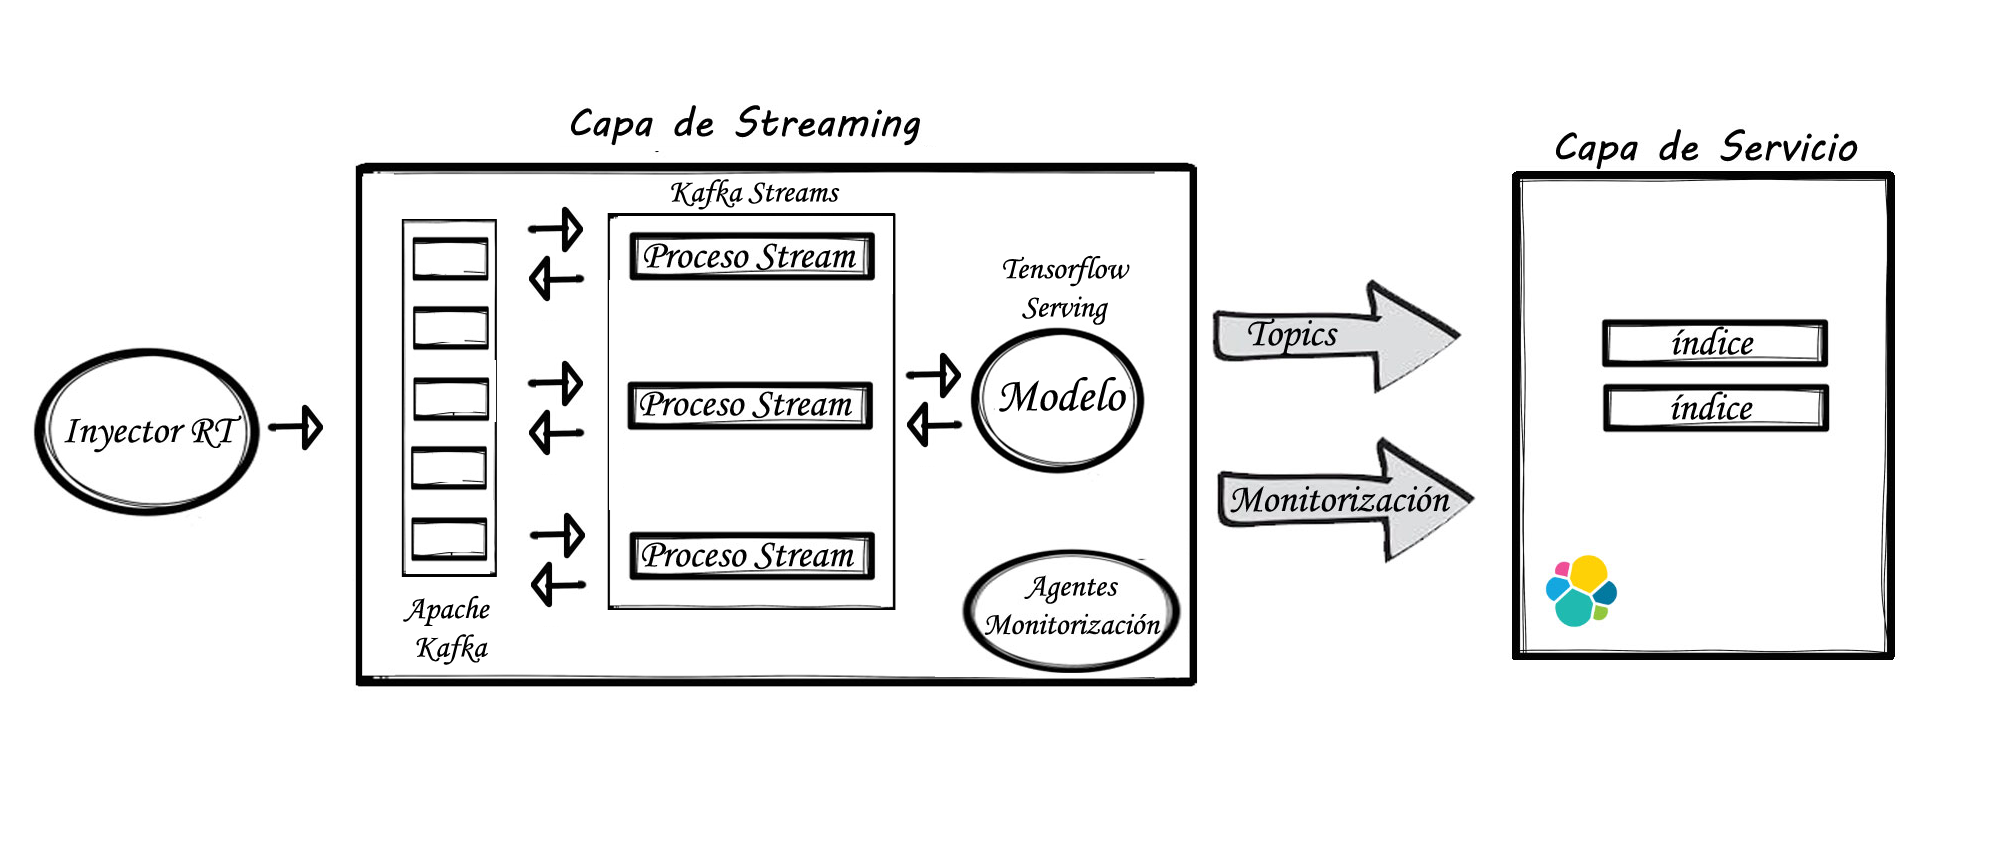
\includegraphics[width=1\textwidth]{images/exp/streaminglayer_v1}
	\caption{Capa de \textit{streaming}}
	\label{fig:streamlayer}
\end{figure}


En la figura \ref{fig:streamlayer} podemos ver un \textit{zoom} de la capa de \textit{streaming} de nuestra arquitectura que describiremos a lo largo del capítulo. 



\section{Requisitos del sistema productivo}
\label{section:prod:req}

En esta primera sección, antes de empezar con la definición de la capa de \textit{streaming}, vamos a recapitular los requisitos que deberá cumplir el sistema encargado de clasificar las llamadas recibidas del \textit{call center} en tiempo real. 

\begin{itemize}
	\item \textbf{Tiempo real}: El sistema debe ser capaz de clasificar las llamadas en tiempo real con una latencia máxima del orden de segundos. 
	\item \textbf{Escalabilidad}: El sistema debe poder escalar horizontalmente de modo que pueda responder en un futuro a un número de llamadas mayor. 
	\item \textbf{Alta disponibilidad}: El sistema debe estar siempre disponible sin que exista en el mismo un punto único de fallo (SPOF , \textit{Single Point Of Failure}).
	\item \textbf{Integración y despliegue continuos}: La integración y el despliegue del sistema deben ser continuos. Esto significa que una vez subido el código a un gestor de versiones deben poder realizarse de manera automática las pruebas necesarias, la compilación y el despliegue del sistema.
	
\end{itemize}

A lo largo del capítulo veremos como la aplicación cumple con los tres primeros puntos: tiempo real, escalabilidad y alta disponibilidad. El cuarto punto referente a la integración y el despliegue continuo se tratará de manera individual en el capítulo \ref{chapter:mant}.

\section{Arquitectura del sistema}


Al abordar la construcción del sistema hemos decidido usar una \textbf{arquitectura de microservicios}, cada uno de los cuales ejecute una parte del proceso. A la hora de diseñar estos microservicios hemos tenido en cuenta que cada uno ejecute una unidad de \textit{software} que tenga sentido por si misma y que pueda ser actualizada, sustituida o utilizada por terceros de una forma independiente. 

Una idea fundamental que subyace detrás de toda arquitectura de microservicios, es que cada microservicio desempeñe su tarea lo más aisladamente del resto y su comunicación con otros microservicios se realice usando protocolos simples y agnósticos a cualquier tecnología, usualmente el protocolo HTTP mediante API REST. 

Sin embargo el uso del protocolo HTTP tiene una serie de implicaciones que pueden no ser muy ventajosas para un sistema que requiere un procesamiento en tiempo real y que busca la simplicidad, como son la sincronía y y el acoplamiento con otros microservicios. La sincronía nos lleva a tener que ``preguntar'' constantemente a un microservicio sobre la existencia de nuevos datos, lo que, desde el punto de vista del rendimiento, implica que el \textit{thread} encargado del procesamiento deba esperar la respuesta HTTP antes de seguir con el procesamiento (esta perdida de rendimiento variará en función del tiempo de procesamiento necesario del microservicio llamado y de la latencia de la red).  Por otro lado, una arquitectura en la que los microservicios se comuniquen mediante REST implica un mínimo de acoplamiento, debido a que los microservicios deben conocer la existencia unos de otros, traduciéndose en una mayor complejidad a la hora de la orquestación de los mismos. 


Es por ello que una solución más optima para nuestro sistema consiste en combinar los beneficios de las arquitecturas \textit{event-driven} con los beneficios de los microservicios utilizando una \textbf{arquitectura de microservicios  \textit{event-driven} (EDM)}. Para desarrollar la arquitectura propuesta, necesitaremos un sistema de mensajería o \textit{streaming} por el que ``viajen'' los eventos y gracias al cual los microservicios puedan comunicarse entre sí. En nuestro caso hemos optado por utilizar \textbf{Apache Kafka como bus central de eventos}. 

El uso de Apache Kafka solventa los inconvenientes planteados por la arquitectura \textit{REST} eliminando la sincronía y el acoplamiento. Por un lado, los microservicios que tienen como origen un bus de mensajería son por naturaleza asíncronos, lo que implica que realizarán el procesamiento de los eventos en el momento que estos sean publicados en el bus; eliminando la necesidad de tener que ``preguntar'' por nuevos eventos y aumentando el rendimiento. Por otro lado, el uso de Apache Kafka hace que los microservicios estén totalmente desacoplados entre sí, eliminando la necesidad de que un microservicio conozca siquiera la existencia del resto. 

Además la arquitectura propuesta nos aporta otras características ventajosas para nuestro proyecto:

\begin{itemize}
	\item \textbf{Reprocesamiento}: Gracias a la capacidad de retención del bus, tenemos la posibilidad de reprocesar los mensajes pasados de ser necesario (p.e. para solventar errores de código).  
	\item \textbf{Alta disponibilidad}. El sistema es tolerante a fallos. Los datos se encuentran en el bus con un número de réplicas que evita la pérdida de los mismos ante caídas de nodos.
	\item \textbf{Escalabilidad}: Apache Kafka nos da la posibilidad de dividir nuestros \textit{topics} en particiones que pueden ubicarse en diferentes nodos. Esto nos proporciona escalabilidad horizontal tanto desde el punto de vista del almacenamiento como del cómputo.
	\item\textbf{ Soportar picos de carga}: Al existir una retención en el bus, en el caso de que ocurriese un pico en el número de eventos recibido que no puedan ser abordados por los procesadores, estos podrán ir procesando la información según su capacidad.
	\item \textbf{Evento en el centro}: Este tipo de arquitectura hace que diseñemos nuestras aplicaciones situando al evento, al dato, en el centro de nuestro sistema.
\end{itemize}


Sin embargo, aunque el uso de este tipo de microservicios  \textit{event-driven} (EDM) posea todas estas ventajas, es cierto que también hay que asumir que el uso de REST está muy implementado actualmente y muchas aplicaciones poseen un API REST \textit{out-of-the-box}. Esto nos llevará como veremos en el siguiente apartado a incorporar microservicios REST en nuestro modelo \textit{event driven}, creando en cierto modo una arquitectura híbrida.





\section{Microservicios}
En la sección anterior decidimos el modelo de arquitectura que vamos a utilizar para construir nuestro sistema, en esta sección nos centraremos en los microservicios que compondrán esa arquitectura.  

\subsection{Tecnología}
En el apartado \ref{section:arqu:tecn} hicimos un repaso por las tecnologías usadas en el proyecto, en este punto queremos tratar de profundizar con un poco más de detalle en las tecnologías que nos permitirán desarrollar y desplegar nuestros microservicios. Estas tecnologías son Kafka Streams y Tensorflow Serving.

\subsubsection{Kafka Streams}

El núcleo de nuestra capa de \textit{streaming} estará compuesto por microservicios desarrollados mediante 
 Kafka Streams. Kafka Streams \cite{kstreams} es una librería cliente que nos permite desarrollar aplicaciones y microservicios  cuya entrada y salida sea un bus Kafka. 
 
 Kafka Streams nos permite desarrollar aplicaciones en \textit{Java} (el lenguaje que usaremos) o Scala de una manera sencilla e intuitiva, además, a diferencia de otros \textit{frameworks} de procesamiento en tiempo real, como puede ser Spark Streaming, no tiene necesidad de disponer de un clúster aparte (usa el mismo bus Apache Kafka) lo que simplifica bastante nuestra arquitectura. Además Kafka Streams nos permitirá \textbf{garantizar la escalabilidad y la tolerancia a fallos} de nuestros despliegues. 
 
 Kafka Streams posee dos APIs diferentes: Processor API y  Streams DSL.  Processor API nos proporciona una capacidad a muy bajo nivel para definir la lógica de nuestro proceso \textit{streaming}; en cambio \textit{DSL}, que esta construido sobre  Processor API, nos permite de una manera sencilla, con un lenguaje declarativo, realizar la mayoría de operaciones posibles en un proceso de \textit{streaming}. Es por ello que en nuestros servicios utilizaremos principalmente \textbf{Streams DSL}, aunque en algún momento tengamos que recurrir a la Processor API para realizar tareas más avanzadas.
 
Una característica interesante de Streams DSL es la existencia de las denominadas KTables que nos permiten usar el Bus como si de una BBDD NoSQL Clave-Valor se tratara. Las Ktables utilizan un \textit{topic} de Apache Kafka, pero al acceder a ellas solo accedemos al último registro disponible para cada clave. Esta característica suele usarse sobre \textit{topics} compactos sin límite de retención, que son aquellos que periódicamente  borran las versiones antiguas de cada clave y retienen, de forma ilimitada, las versiones más recientes. Esta posibilidad nos permitirá cargar en el bus las tablas de \textit{lookup} necesarias para enriquecer registros en nuestro procesamiento y eliminará las dependencias de nuestro flujo con BBDD externas. 


 
 
\subsubsection{\textit{Tensorflow Serving}}

\textit{Tensorflow Serving} \cite{tfserving} está pensado para llevar a producción los modelos que hemos creado con \textit{Tensor Flow}, pudiéndose adaptar también para otros modelos. Tensorflow Serving nos permite desplegar nuestros modelos y algoritmos manteniendo intacta la API de consulta, esto lo hace ideal para entornos en los que queremos ir actualizando las versiones de nuestros modelos sin modificar el resto del sistema.

Los modelos desplegados con Tensorflow Serving pueden consultarse a través de un \textit{API} en C++ o mediante un \textbf{API REST} que es la opción escogida por nosotros debido a que, por la simplicidad del protocolo, es la que más encaja con nuestra arquitectura de microservicios. 

Una característica interesante de \textit{Tensorflow Serving}  es el \textbf{versionado}, ya que nos permite servir en paralelo varias versiones de un modelo, algo que puede ser muy interesante para, por ejemplo, realizar un test A/B.





\subsection{Microservicios}

Una vez determinada la arquitectura del sistema y las tecnologías escogidas para su implementación es el momento de diseñar los microservicios necesarios para nuestro caso de uso.

El primer paso es localizar las funciones básicas que queremos que realice nuestro sistema agrupadas en dos grandes etapas: preprocesamiento y predicción. La etapa de preprocesamiento será la encargada de preparar las llamadas para que puedan convertirse en la entrada de nuestro modelo, mientras que la etapa de predicción será la encargada de aplicar el modelo. 

Dentro de la etapa de preprocesamiento es necesario, en un primer lugar, la extracción de los \textit{tokens} de la transcripción de llamada, de esto se encargará un microservicio que hemos denominado \textit{\textbf{Tokenizer}}. Una vez obtenidos los \textit{Tokens} también será necesario, para que puedan convertirse en entrada del modelo, transformarlos en una secuencia numérica; esto será realizado por otro microservicio denominado \textit{\textbf{Sequencer}}.

Por último en la capa de predicción son necesarios otros dos pasos: por un lado aplicar el modelo  obteniendo una probabilidad de pertenencia a cada clase, de esto se encargará un microservicio denominado \textbf{\textit{tf-BajaFactura}} y, por otro lado, enriquecer estas predicciones con las etiquetas necesarias y enriquecer la salida del microservicio anterior; esto será responsabilidad de un microservicio denominado \textbf{\textit{Predicter}}. Como podemos imaginar por la definición, existirá un ligero acoplamiento entre estos dos microservicios, que comentaremos a lo largo de esta sección.
\vspace{0.2cm}

\begin{figure}[!ht]
	\centering
	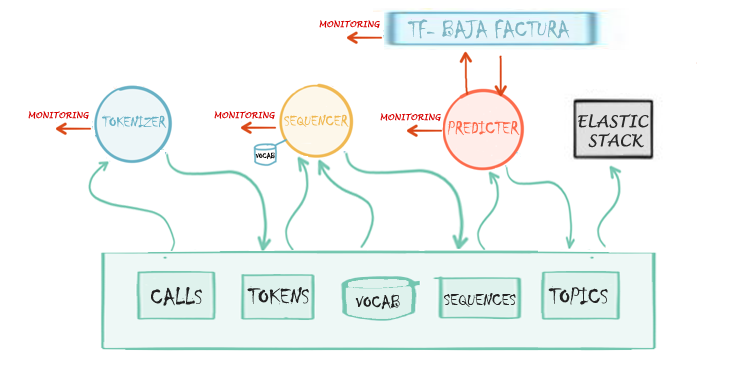
\includegraphics[width=1\textwidth]{images/exp/micro-arch-v3}
	\caption{Arquitectura microservicios}
	\label{fig:micro-arch}
\end{figure}


En la figura \ref{fig:micro-arch} podemos ver como los microservicios propuestos interactúan entre sí a través del bus, con excepción del microservicio  \textbf{\textit{tf-BajaFactura}}. Estos microservicios conforman la parte capa de \textit{streaming} de nuestro sistema. En el capítulo siguiente veremos como la salida de esta capa de \textit{streaming} alimentará la capa de servicio.


A continuación, en los siguientes subapartados describiremos uno a uno los diferentes microservicios. 


\subsection{\textit{Tokenizer}}

Este microservicio tiene como entrada las llamadas transcritas que llegan al bus en tiempo real. A partir del texto de las mismas el sistema inicia un proceso de \textit{tokenizacion} eliminando \textit{stopwords}, carácteres especiales (signos de puntuación, 'ñ's, acentos...), palabras comunes, números, nombres propios y pasando a minúscula cada uno de los tokens.  El proceso de \textit{tokenización} pretende ser lo más fiel posible al proceso realizado en \textit{Python} durante la etapa de entrenamiento del modelo.

Una vez obtenida la lista de \textit{tokens} esta se vuelve a disponibilizar en el bus en un nuevo \textit{topic}. Este nuevo \textit{topic} con las llamadas \textit{tokenizadas} puede ser de utilidad no solo para nuestro sistema, si no también para cualquier otro sistema de análisis de texto que necesite partir de los datos \textit{tokenizados}.

El \textit{topic} de entrada del microservicio  \textit{Tokenizer}, llamado \textit{CALLS}, tendrá como clave el código de la llamada y como cuerpo un objeto \textit{json} con los siguientes campos:

\begin{itemize}
		\item \textbf{\textit{co\_verint}} : Código de la llamada. 
		\item  \textbf{\textit{call\_text}} : Texto de la llamada. 
		\item  \textbf{\textit{call\_timestamp}}: Hora de la llamada.
        \item \textbf{\textit{province}}: Provincia desde la que se ha realizado la llamada. 
        \item \textbf{\textit{co\_province}}: Código de provincia desde la que se ha realizado la llamada. 
        \item \textbf{\textit{duration}}: Duración en segundos de la llamada. 
        \item \textbf{\textit{control\_type}}: De existir, tipo de llamada (usado para el proceso de verificación). 
\end{itemize} 

Como salida escribirá en un \textit{topic}  llamado \textit{TOKENS.CALLS} un evento cuya clave será el código de la llamada y cuyo cuerpo un objeto \textit{json} con los siguientes campos:

\begin{itemize}
		\item \textbf{\textit{co\_verint}} : Código de la llamada. 
		\item  \textbf{\textit{call\_text}} : Texto de la llamada. 
		\item  \textbf{\textit{call\_timestamp}}: Hora de la llamada.
        \item \textbf{\textit{province}}: Provincia desde la que se ha realizado la llamada. 
        \item \textbf{\textit{co\_province}}: Código de provincia desde la que se ha realizado la llamada. 
        \item \textbf{\textit{duration}}: Duración en segundos de la llamada. 
        \item \textbf{\textit{control\_type}}: De existir, tipo de llamada (usado para el proceso de verificación).  
        \item \textbf{\textit{tokens}}: Lista de tokens extraída de \textit{call\_text}. 
\end{itemize} 



\subsection{\textit{Sequencer}}
Este microservicio toma como entrada la salida del microservicio anterior y a partir de la lista de \textit{tokens} devuelve una secuencia de tamaño fijo determinado $T$. Para ello, utiliza un diccionario en el que cada \textit{token} se corresponde con un número, utilizando el $0$ para \textit{tokens} que no existan en este diccionario. Esta secuencia esta limitada a un tamaño determinado $T$, por lo que llamadas con un número mayor de $tokens$ son recortadas y se utiliza \textit{padding} por la izquierda para completar la secuencia de llamadas con un tamaño menor a $T$.

El diccionario ha sido calculado sobre el conjunto de datos de  entrenamiento y contiene el vocabulario del modelo. Este diccionario contiene como clave todos los \textit{tokens} posibles y como valores el identificador usado para cada \textit{token}. La lectura del mismo se realiza desde el mismo bus, utilizando la funcionalidad \textit{KTable} de \textit{Kafka Streams}.


Una vez obtenida la secuencia de caracteres, esta se disponibiliza en un nuevo \textit{topic} del bus. Además de por nuestro sistema, este valor puede ser consumido por otros microservicios o sistemas que tengan como objetivo aplicar diferentes modelos a las secuencias obtenidas.

El \textit{topic} de entrada del microservicio \textit{Sequencer} será el topic  \textit{TOKENS.CALLS} descrito en el apartado anterior. 

Como salida escribirá en un \textit{topic}  llamado \textit{SEQUENCES.CALLS} un evento cuya clave será el código de la llamada y cuyo cuerpo un objeto \textit{json} con los siguientes campos:

\begin{itemize}
		\item \textbf{\textit{co\_verint}} : Código de la llamada. 
		\item  \textbf{\textit{call\_text}} : Texto de la llamada. 
		\item  \textbf{\textit{call\_timestamp}}: Hora de la llamada.
        \item \textbf{\textit{province}}: Provincia desde la que se ha realizado la llamada. 
        \item \textbf{\textit{co\_province}}: Código de provincia desde la que se ha realizado la llamada. 
        \item \textbf{\textit{duration}}: Duración en segundos de la llamada. 
        \item \textbf{\textit{control\_type}}: De existir, tipo de llamada (usado para el proceso de verificación).  
        \item \textbf{\textit{sequence}}: Lista de 866 enteros en el que cada uno representa el identificador de un \textit{token}. La secuencia se completa con ceros en caso de ser necesario.
\end{itemize} 


Además se apoyará en un topic compacto que no tendrá  límite de retención, denominado \newline \textit{TBL.VOCABULARY.CALLS}, cuya clave son los \textit{tokens} existentes en el vocabulario y,  cuyo  valor es un identificador para cada uno de ellos.

\subsection{\textit{tf-BajaFactura}}
\textit{\textbf{tf-BajaFactura}} quizás sea el microservicio más tradicional y discordante de los que vamos a utilizar en nuestro sistema debido a que este microservicio se encuentra totalmente desacoplado del bus y del resto de microservicios. Mediante un API REST aplica nuestro modelo de TensorFlow a una o varias secuencias de entradas y, para cada secuencia, devuelve la probabilidad de pertenencia a las clases: ``Baja'', ``Factura'' y ``Resto''.

El motivo principal para usar API REST en este microservicio se debe al uso de la tecnología  Tensorflow Serving comentada en el capítulo anterior y que nos permite con mucha facilidad desplegar nuevos modelos y algoritmos, manteniendo la misma estructura en el servidor y la misma API. Además su integración es automática con los modelos generados con TensorFlow (con o sin Keras). Esta decisión permite a los \textit{data-scientist} desplegar nuevas versiones de sus modelos, ya sea por degradación o por mejora, mientras el resto del flujo permanece inalterable. 

La entrada del modelo \textit{tf-BajaFactura} será un documento \textit{json} que contenga el campo \textit{instances} compuesto por una lista de secuencias. En nuestro caso una sola secuencia, ya que el modelo será llamado con cada evento recibido. La salida será también en \textit{json} y contendrá una lista de predicciones, en cada predicción tendremos la probabilidad de pertenencia a cada clase.




\subsection{Predicter}
Este último microservicio tiene como entrada el \textit{topic} generado por \textit{\textbf{Sequencer}} y a partir del mismo realiza una llamada a \textit{\textbf{tf-BajaFactura}}. Una vez obtenidas las predicciones, las enriquece con las etiquetas necesarias. Además en el caso de existir un atributo de control comprueba si la predicción ha sido correcta, esto nos servirá para validar la eficiencia del modelo a lo largo del tiempo. 

Como podemos observar, es el único microservicio que tiene una dependencia con otro (\textit{tf-BajaFactura}), sin embargo la API de un modelo implementado con Tensorflow Serving \cite{tfserving} es siempre idéntica. Esto provoca que la llamada no varíe aunque cambie el modelo. Además, en el servicio \textit{\textbf{Predicter}}, el número de clases y las etiquetas de las mismas son configurables , pudiendo  reutilizarse este microservicio para cualquier servicio predictivo desplegado mediante  Tensorflow Serving.

La salida de este microservicio es publicada en un nuevo \textit{topic} en el bus, esta información puede ser de utilidad para diversos sistemas que quieran realizar analítica en función de la temática de las llamadas o que quieran visualizarla. Nosotros la usaremos en nuestra capa de servicio que describiremos en el siguiente capítulo.

El \textit{topic} de entrada del microservicio \textit{Predicter} será el topic  \textit{SEQUENCES.CALLS} descrito en el servicio \textit{Sequencer}. 


Como salida escribirá en un \textit{topic}  llamado \textit{TOPICS.CALLS} un evento cuya clave será el código de la llamada y cuyo cuerpo un objeto \textit{json} con los siguientes campos:

\begin{itemize}
		\item \textbf{\textit{co\_verint}} : Código de la llamada. 
		\item  \textbf{\textit{call\_text}} : Texto de la llamada. 
		\item  \textbf{\textit{call\_timestamp}}: Hora de la llamada.
        \item \textbf{\textit{province}}: Provincia desde la que se ha realizado la llamada. 
        \item \textbf{\textit{co\_province}}: Código de provincia desde la que se ha realizado la llamada. 
        \item \textbf{\textit{duration}}: Duración en segundos de la llamada. 
        \item \textbf{\textit{control\_type}}: De existir, tipo de llamada (usado para el proceso de verificación).  
        \item  \textbf{\textit{predictions}}: Lista con las predicciones devueltas por el servicio  \textit{tf-BajaFactura}. 
        \item  \textbf{\textit{error}}: De producirse, contendrá el error devuelto por el  servicio  \textit{tf-BajaFactura} o el error de conexión con el mismo.      
         \item  \textbf{\textit{model}}: ID del modelo aplicado, en nuestro caso siembre será BajaFactura.
         \item  \textbf{\textit{pred\_type}}: Etiqueta de la clase más probable según la predicción.
         \item  \textbf{\textit{control\_success}}: En el caso de existir el campo \textit{control\_type}, \textit{Booleano} que nos indica si la predicción ha sido correcta.
\end{itemize} 


\section{Monitorización de Microservicios}

Si bien es cierto que el hecho de utilizar una arquitectura orientada a eventos, aparte de la sencillez intrínseca de nuestro sistema, nos simplifica en cierto modo la orquestación de nuestro servicios y nos permite prescindir de herramientas de APM (\textit{Application Performance Monitoring}); una monitorización del desempeño de nuestros microservicios es siempre necesaria, tanto para garantizar el correcto funcionamiento de los mismos y poder detectar posibles puntos de fallo, como para detectar pérdidas de rendimiento en cualquier punto del sistema. 

En esta sección veremos los métodos utilizados para monitorizar los microservicios dependiendo de su tecnología. 


\subsection{Servicios \textit{Kafka Streams}}

Los servicios de Kafka Streams corren sobre la máquina virtual de Java lo que nos permite tener acceso a sus métricas por medio de la JMX(\textit{Java Management Console}). Ademas Confluent posee una documentación de los MBeans y de las métricas que contienen en su documentación oficial \cite{monitoringstreams}. 


El inconveniente de estas métricas es que tienen que extraerse por medio de protocolos RMI (\textit{Java Remote Method Invocation}) lo que complica su explotación, sin embargo a partir de la versión 6 del JDK (\textit{Java Development Kit}) tenemos la posibilidad de exportar estas métricas de JMX directamente mediante API REST. Esto nos da la posibilidad de poder recolectar las métricas directamente mediante una llamada HTTP.

Para recolectar estás métricas utilizaremos los Beats de  Elastic, concretamente Metricbeat. Este será el encargado de recolectar las métricas necesarias y enviarlas a Logstash para su posterior almacenamiento en Elasticsearch. El flujo de Logstash a Elasticsearch lo trataremos con más detalle en el próximo capítulo en el que veremos la capa de servicio, ya que las métricas de monitorización seguirán el mismo recorrido que los datos de clasificación. 


De todas las métricas disponibles de Confluent, nosotros extraeremos con una frecuencia de un minuto las siguientes métricas:

\begin{itemize}
	\item \textit{mbean 'java.lang:type=Runtime'} : Métrica \textit{Uptime}.
	
	\item \textit{mbean 'kafka.streams:type=stream-metrics'}: Métricas \textit{process-latency-avg}, \textit{process-latency-max} y \textit{process-rate}.
\end{itemize}



Esto nos permitirá para cada microservicio tener información del tiempo de servicio del mismo, de la latencia máxima y media de procesamiento de los eventos y de la tasa de procesamiento. 





\subsection{Servicios \textit{Tensorflow Serving}}

En el caso de la monitorización del servicio \textit{tf-BajaFactura}, habilitaremos la monitorización de Prometheus de Tensorflow Serving para que las métricas sean accesibles mediante API REST, pero en lugar de utilizar Prometheus (para no incluir complejidad en nuestro sistema), usaremos directamente el \textit{Input} \textit{Http\_poller} de Logstash.

De todas las métricas disponibles en Tensorflow Serving nos quedaremos unicamente con: 

\begin{itemize}
\item \textbf{Estado}: Que nos dará información sobre si el modelo ha sido cargado con éxito y se encuentra operativo.  

\item \textbf{Total peticiones}: Total de peticiones resueltas por el modelo.

\item \textbf{Total nanosegundos del grafo}: El total de tiempo que el modelo ha dedicado en procesar todas las peticiones. Utilizaremos el total de peticiones para extraer la latencia media y lo expresaremos en milisegundos. 

\end{itemize}




Una vez recolectadas las métricas y enviadas a Logstash, seguirán el mismo flujo descrito en el apartado anterior hacia la capa de servicio, este flujo será tratado en más detalle en el capítulo siguiente. 

Además de las métricas recolectadas, la monitorización del microservicio \textit{\textbf{predicter}} nos dará información combinada de ambos ya que internamente realiza una llamada a \textit{tf-BajaFactura}.



\section{Inyector: simulador de tiempo real}
Como ya hemos comentado en anteriores capítulos actualmente las transcripciones de las llamadas no se encuentran disponibles en tiempo real, es por ello que se ha diseñado un inyector de llamadas.

Este inyector, realizado en Python utiliza como fuente la transcripción de las llamadas realizadas en batch. Y a partir de la misma cumplirá los siguientes objetivos: 

\begin{itemize}
	\item \textbf{ Extraer la frecuencia de llamadas por hora}. De este modo simularemos el comportamiento real de un \textit{call center} inyectando más llamadas a las horas del día con mayor actividad.
	\item \textbf{Multiplicar el número de llamadas}. Teniendo en cuenta que actualmente solo se transcriben un 4\% del total de las llamadas, el inyector multiplicará por 25 el número de llamadas recibidas en un día para simular el comportamiento real de un sistema que ingeste el 100\% de las llamadas.
	\item \textbf{Introducir datos de control}: El inyector insertará en un porcentaje de llamadas los datos reales de clasificación con el fin de poder verificar el comportamiento del modelo. En un entorno real se podrían insertar periódicamente un número de llamadas de control que nos permitan este objetivo.
	
\end{itemize}

Una vez realizadas estas tareas, el inyector publicará todas las llamadas al bus, simulando un comportamiento real. De este modo las llamadas estarán disponibles en tiempo real para cualquier consumidor que las necesite.

Aunque el inyector podría verse como un microservicio más, hemos preferido dejarlo fuera del sistema a lo largo de todo el apartado, debido a que lo consideramos una pieza auxiliar que nos permite simular el comportamiento real del sistema sin disponer de los datos en este momento.


\chapter{Capa de servicio}
\label{chapter:servicio}

\section{Carga y modelo}


\section{Visualizaciones}

\subsection{Monitorización}
\subsection{Sistema}

\section{Alarmado}





\chapter{Despliegue en contenedores}
Una vez desarrollados los microservicios y su monitorización, es necesario ponerlos en producción, y una de las decisiones importantes es dónde queremos que corran, si en máquinas físicas, máquinas virtuales o en contenedores (en nuestro caso, se descarta la opción de implementarlo en \textit{Cloud}). La decisión tomada es que todo corra sobre contenedores en una plataforma \textit{\textbf{OCP}} \textit{Openshift Container Platform}, los motivos de esta decisión son los siguientes: 

\begin{itemize}
	\item \textit{\textbf{Stateless}}: Todos los servicios implementados no necesitan estado (los datos necesarios se almacenan en el bus). Lo que lo hace un caso de uso ideal para su ejecución en contenedores. 
	\item \textbf{Agilidad de despliegue}: El proceso de creación y destrucción de un contenedor es inmediato, lo que no da mucha flexibilidad a la hora desplegar nuevos contenedores.
	
	\item \textbf{Serivicios Autocontenidos}: Los contenedores pueden ejecutarse en multitud de plataformas lo que nos permite tener aplicaciones inmutables y autocontenidas que podemos mover entre plataformas y entornos. Este punto y el anterior serán de mucha utilidad a la hora de implementar la integración y el despliegue continuo.
	
	\item  \textbf{Alta disponibilidad}: Al tener un clúster de \textit{Openshift} con múltiples nodos, en el caso que se produjera un fallo en un nodo que provocara la caída de un contenedor, este se levantaría automáticamente en otro nodo. 
	
\end{itemize} 

A la largo del apartado nos referiremos a los siguientes conceptos propios de \textit{Openshift} (muchos de ellos heredados en \textit{Kubernetes}):

\begin{itemize}
\item  \textit{\textbf{Pod}}: Un pod es la unidad mínima en \textit{OCP}. Puede estar formado por uno o varios contenedores (\textit{Docker}), pero todos ellos correrán en una única máquina y tendrán una única dirección IP.

\item  \textit{\textbf{Despliegue}}: Un despliegue (\textit{Deployment}) podemos decir, de una manera muy simplificada, que gestiona el número de réplicas de un \textit{pod}. 

\item  \textbf{Configuración de despliegue}: La configuración de despliegue (\textit{Deployment Config}) dota a los despliegues de un ciclo de vida proporcionando versiones de los mismo, disparadores para crear nuevos despliegues de manera automática y estrategias para realizar transiciones entre diferentes versiones de despliegues sin pérdida de servicio. 

\item  \textbf{Servicio}: Un servicio expone un número determinado de Pods para que sean accesibles desde otros elementos de la plataforma. 

\item  \textbf{\textit{ConfigMap}}: Se trata de un mecanismo de \textit{OCP} para almacenar elementos de configuración mediante un mecanismo de clave-valor. Es posible almacenar tanto ficheros como valores simples.


\end{itemize}

\begin{figure}[!ht]
	\centering
	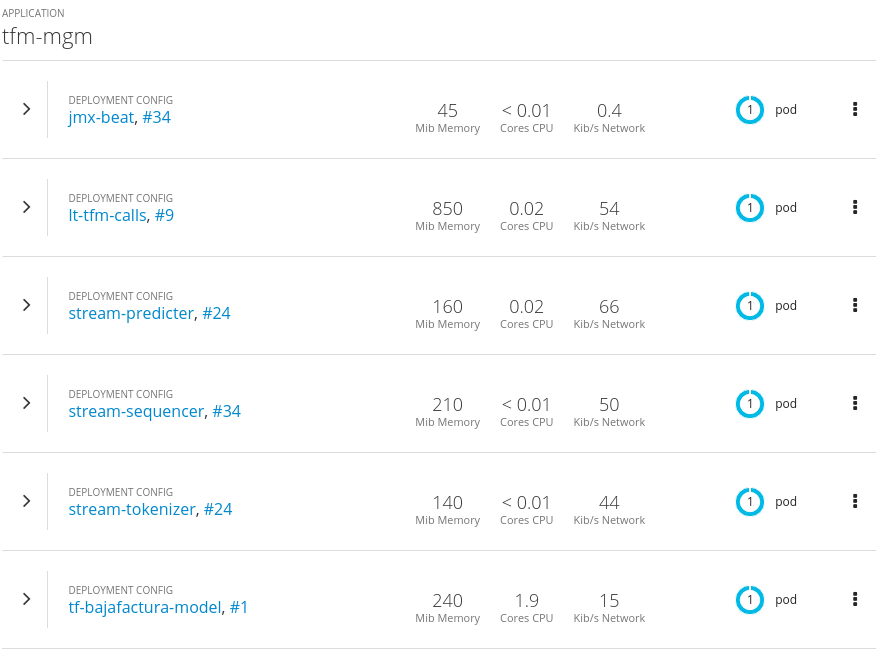
\includegraphics[width=1\textwidth]{images/cont/overview}
	\caption{configuración de despliegue y recursos usados en OCP}
	\label{fig:ocp-overview}
\end{figure}

En la figura \ref{fig:ocp-overview} podemos ver las diferentes configuraciones de despliegue con los \textit{pods} que tienen levantados cada uno y los recursos de memoria, cpu y red que consumen cada uno. 
 
A continuación veremos un resumen de los servicios, despliegues y configuraciones desplegadas en Openshift para cada tipo de microservicio y monitorización. En el apéndice \cite{apendi:contenedores} podemos encontrar todo el código de despliegue en Openshift, que nos permitiría desplegar todo nuestro entorno en otro clúster en cuestión de minutos. 


\section{Servicios \textit{Kafka Streams}}

Para desplegar los servicios de \textit{Kafka Streams} en \textit{OCP} es necesario desplegar una  configuración de despliegue por microservicio, un servicio para exponer las métricas y disponer en un \textit{configmap} de las opciones necesarias para su ejecución. 

En este apartado únicamente presentaremos a modo de ejemplo la configuración de despliegue y el servicio  del microservicio \textit{Predicter} explicando las características más relevantes del mismo. Tanto el \textit{configmap} con todos los ficheros como el resto de despliegues pueden consultarse en el apéndice \cite{apendi:contenedores}. 

La configuración de despliegue de \textit{Predicter} es la siguiente: 

\begin{minted}[
	gobble=0,
	frame=single,
	linenos
	]{yaml}

apiVersion: apps.openshift.io/v1
kind: DeploymentConfig
metadata:
  labels:
    app: tfm-mgm
    project: topic-model
    service: stream-predicter
  name: stream-predicter
  namespace: nbia-prod
spec:
  replicas: 1
  revisionHistoryLimit: 10
  selector:
    deploymentconfig: stream-predicter
  strategy:
    activeDeadlineSeconds: 21600
    recreateParams:
      timeoutSeconds: 600
    resources: {}
    type: Recreate
  template:
    metadata:
      creationTimestamp: null
      labels:
        app: tfm-mgm
        deploymentconfig: stream-predicter
        project: topic-model
        service: calls-predicter
    spec:
      containers:
        - env:
            - name: JAVA_MAIN_CLASS
              value: com.telefonica.topicmodel.PredicterLauncher
          image: >-
            docker-registry.default.svc:5000/nbia-prod/
            topic-model-streaming:latest
          imagePullPolicy: Always
          name: stream-predicter
          ports:
            - containerPort: 8778
              protocol: TCP
          resources:
            limits:
              cpu: '1'
              memory: 512Mi
            requests:
              cpu: 200m
              memory: 256Mi
          terminationMessagePath: /dev/termination-log
          terminationMessagePolicy: File
          volumeMounts:
            - mountPath: /opt/jolokia/etc/jolokia.properties
              name: calls-config
              subPath: jolokia.properties
            - mountPath: /deployments/application.json
              name: calls-config
              subPath: topic-model-streaming.json
      dnsPolicy: ClusterFirst
      restartPolicy: Always
      schedulerName: default-scheduler
      terminationGracePeriodSeconds: 30
      volumes:
        - configMap:
            defaultMode: 420
            name: calls-config
          name: calls-config
  test: false
  triggers:
    - imageChangeParams:
        automatic: true
        containerNames:
          - stream-predicter
        from:
          kind: ImageStreamTag
          name: 'topic-model-streaming:latest'
          namespace: nbia-prod
      type: ImageChange
    - type: ConfigChange

\end{minted}

Del despliegue anteriormente expuesto podemos destacar las siguientes características: 

\begin{itemize}
	\item \textbf{labels} (línea 4):  Nos ayudan a identificar el despliegue, el proyecto y la aplicación. Todos los despliegues relacionados con el TFM que se presentan en este documento tendrán el indicador \textit{tfm-mgm}. 

	\item \textbf{replicas} (línea 11): Indica el número de réplicas de cada \textit{pod} que pueden correr al mismo tiempo. En este caso lo establecemos a uno, pero podría escalar horizontalmente incluso hacerlo de manera automática por uso de CPU o memoria mediante un \textit{Horizontal Pod Autoscaler}. 



	\item \textbf{strategy} (línea 15): Establecemos la estrategia con la que se implantará una nueva versión del \textit{deployment}, en este caso utilizamos una estrategia \textit{Recreate} que detiene todos los servicios de un \textit{deployment} anterior antes de iniciar uno nuevo. Debido a que el bus tiene capacidad de retención de los eventos, esto no implicará una interrupción en el servicio, si no un ligero retraso en los eventos que se ingesten durante el despliegue.

	\item \textbf{Container} (línea 30): Aquí encontramos toda la información del contenedor que se desplegará. Destacamos: 
		\begin{itemize}
			\item \textbf{env} (línea 31): Variables globales del \textit{deploynment}, en este caso la clase Java  principal que se lanzará al ejecutar el contenedor. 
			\item \textbf{image} (línea 34): Contiene la referencia a la imagen del contenedor que queremos desplegar. Se trata de una imagen de Java con nuestro código que se encuentra almacenada en el repositorio de la plataforma. El parámetro \textit{imagePullPolicy} indica en qué circunstancias se descargará la imagen del repositorio (en este caso lo hará siempre, exista o no en el nodo en el que se despliega el \textit{Pod}).
			\item \textbf{Ports} (línea 34): Indica los puertos que expondrá el contenedor, en este caso se expondrá únicamente el puerto 8778 que es el puerto por defecto del \textit{endpoint} de \textit{Jolokia}.
			\item \textbf{Resources} (línea 42): Contiene los recursos de CPU y memoria que solicitará el \textit{Pod}  al arrancar y a los que estara limitados. 
			\item \textbf{VolumeMounts} (línea 51): Indica los volúmenes que montará el contenedor, en este caso son todos procedentes de un \textit{configmap} y contienen los ficheros de configuración de \textit{jolokia} y de la aplicación.
		\end{itemize}
	\item  \textbf{volumes} (línea 62): Contiene los volúmenes que se utilizaran en los contenedores en el apartado \textit{VolumeMounts}. En este caso unicamente contiene un \textit{configmap}. 
	\item \textbf{triggers} (línea 68): Define los disparadores que provocarán que se realice un nuevo \textit{deployment}, en este caso la modificación de la imagen o la modificación de la configuración de despliegue.

\end{itemize}


El servicio de \textit{Predicter} es el siguiente: 

\begin{minted}[
	gobble=0,
	frame=single,
	linenos
	]{yaml}

apiVersion: v1
kind: Service
metadata:
  labels:
    app: tfm-mgm
  name: stream-predicter
  namespace: nbia-prod
spec:
  ports:
    - name: 8778-tcp
      port: 8778
      protocol: TCP
      targetPort: 8778
  selector:
    deploymentconfig: stream-predicter
  sessionAffinity: None
  type: ClusterIP

\end{minted}

Aparte de las etiquetas que tienen las misma utilidad que la configuración de despliegue vista anteriormente, cabe destacar los siguientes parámetros: 

\begin{itemize}
	\item \textbf{name} (línea 6): El nombre del servicio que usaremos para llamarlo dentro de la plataforma. 
	 \item \textbf{ports} (línea 9): El puerto que expondrá el servicio y al puerto de los \textit{pods} que atacará. 
	 \item \textbf{selector} (línea 14): Los \textit{pods} a los que atacará el servicio. En este caso los \textit{pods} pertenecientes al configuración de despliegue \textit{stream-predicter}. 
	 
	 \item \textbf{sessionAffinity} (línea 16): Si quisieramos establecer alguna afinidad, por ejemplo a nivel de \textit{IP}, para que un mismo origen ataque siempre a un mismo \textit{Pod}. Hay que recordar que los servicios en \textit{Openshift} (y \textit{Kubernetes}) actúan como un balanceador entre los \textit{pods}.
\end{itemize}




\section{Servicios \textit{Tensorflow Serving}}

En el caso del servicio de Tensorflow Serving, mostraremos únicamente la configuración de despliegue, aunque también consta de un servicio para que podamos realizar llamadas \textit{HTTP} sobre el mismo desde la plataforma de \textit{Openshift}. En el caso de que se quisiera acceder al servicio desde fuera de la plataforma será necesario recurrir las \textit{Routes} de Openshift.

La configuración de despliegue de \textit{tf-BajaFactura} es la siguiente:

 
\begin{minted}[
	gobble=0,
	frame=single,
	linenos
	]{yaml}
apiVersion: apps.openshift.io/v1
kind: DeploymentConfig
metadata:
  labels:
    app: tfm-mgm
    appName: tf-bajafactura-model
    appTypes: tensorflow-serving-s2i
    appid: tf-serving-tf-bajafactura-model
  name: tf-bajafactura-model
  namespace: nbia-prod
spec:
  replicas: 1
  revisionHistoryLimit: 10
  selector:
    deploymentconfig: tf-bajafactura-model
  strategy:
    activeDeadlineSeconds: 21600
    rollingParams:
      intervalSeconds: 1
      maxSurge: 25%
      maxUnavailable: 25%
      timeoutSeconds: 600
      updatePeriodSeconds: 1
    type: Rolling
  template:
    metadata:
      labels:
        app: tfm-mgm
        appName: tf-bajafactura-model
        appTypes: tensorflow-serving-s2i
        appid: tf-serving-tf-bajafactura-model
        deploymentconfig: tf-bajafactura-model
    spec:
      containers:
        - env:
            - name: PORT
              value: '8501'
            - name: MODEL_NAME
              value: bajafactura
            - name: RUN_OPTIONS
          image: >-
            docker-registry.default.svc:5000/nbia-prod/
            tf-bajafactura-model:latest
          imagePullPolicy: Always
          livenessProbe:
            failureThreshold: 10
            httpGet:
              path: /v1/models/bajafactura
              port: 8501
              scheme: HTTP
            initialDelaySeconds: 20
            periodSeconds: 30
            successThreshold: 1
            timeoutSeconds: 5
          name: tf-bajafactura-model
          ports:
            - containerPort: 8501
              protocol: TCP
          readinessProbe:
            failureThreshold: 1
            httpGet:
              path: /v1/models/bajafactura
              port: 8501
              scheme: HTTP
            initialDelaySeconds: 20
            periodSeconds: 10
            successThreshold: 1
            timeoutSeconds: 5
          resources:
            limits:
              cpu: '2'
              memory: 2Gi
            requests:
              cpu: '1'
              memory: 1Gi
          terminationMessagePath: /dev/termination-log
          terminationMessagePolicy: File
      dnsPolicy: ClusterFirst
      restartPolicy: Always
      schedulerName: default-scheduler
      terminationGracePeriodSeconds: 30
  test: false
  triggers:
    - imageChangeParams:
        automatic: true
        containerNames:
          - tf-bajafactura-model
        from:
          kind: ImageStreamTag
          name: 'tf-bajafactura-model:latest'
          namespace: nbia-prod
      type: ImageChange
    - type: ConfigChange


\end{minted}

En este caso solo comentaremos los parámetros que varían con respecto al despliegue de los servicios \textit{Kafka Streams}: 
\begin{itemize}
	\item \textbf{strategy} (línea 16): En este caso la estrategia en el caso de que exista un nuevo despliegue se denomina \textit{Rolling}. Esto implica, de forma muy resumida, que el nuevo \textit{deployment} se hará de manera paulatina, no eliminando los \textit{deployment} anteriores hasta que no se hayan realizado los nuevos. Esto garantiza que no exista una pérdida de servicio en los nuevos despliegues.  
	\item \textbf{image} (línea 41): La imagen usada en este caso es la imagen de \textit{docker} de TensorFlow Serving con nuestro modelo cargado, esta imagen  se encuentra almacenada en el repositorio de la plataforma.
	\item \textbf{livenessProbe} (línea 45): Comprueba que el contenedor sigue con vida, de no ser así durante el número de intentos establecido se reiniciará el contenedor. En este caso la comprobación es una petición \textit{HTTP} al \textit{endpoint} de estado del modelo.
	 \item \textbf{readinessProbe} (línea 59): Antes de enviar tráfico a un \textit{pod}, este debe estar en estado \textit{ready}. Con este parámetro establecemos que el \textit{pod} no se encuentre \textit{ready} hasta que no se haya verificado el \textit{endpoint} de estado del modelo.
\end{itemize}

Aunque existen otros parámetros que varían como las variables de entornos o los recursos definidos el funcionamiento es igual a la configuración de despliegue definida anteriormente.


\section{Monitorización}

Los despliegues vistos hasta ahora nos permiten tener funcionando nuestro sistema, sin embargo, no debemos olvidarnos de la monitorización necesaria, que ya describimos en el capítulo \ref{chapter:prod}, para verificar el correcto funcionamiento del mismo. 

Dentro de Openshift la monitorización esta formada por dos despliegues diferentes:

\begin{itemize}
\item \textbf{Logstash}: Podemos identificarlo en la figura \ref{fig:ocp-overview} con el nombre \textbf{lt-tfm-calls} y será el encargado de llevar a la capa de servicio no solo la monitorización de todo el sistema, si no también los datos de clasificación de llamadas y  de realizar las transformaciones necesarias. 

\item \textbf{Metricbeat}: Podemos identificarlo en la figura \ref{fig:ocp-overview} con el nombre \textbf{jmx-beat} y será el encargado de extraer las métricas de Jolokia de los servicios de \textit{Kafka Streams}. 
\end{itemize}

A continuación veremos la configuración de ambos despliegues.

\subsection{Logstash}
Al igual que en los casos anteriores, vemos unicamente la configuración del despliegue, pudiendo encontrar el resto de recursos en el código original.

La configuración de despliegue es la siguiente:

\begin{minted}[
 	gobble=0,
 	frame=single,
 	linenos]{yaml}
apiVersion: apps.openshift.io/v1
kind: DeploymentConfig
metadata:
  labels:
    app: tfm-mgm
    service: lt-tfm-calls
    version: '1.0'
  name: lt-tfm-calls
  namespace: nbia-prod
spec:
  replicas: 1
  revisionHistoryLimit: 10
  selector:
    deploymentconfig: lt-tfm-calls
  strategy:
    activeDeadlineSeconds: 21600
    resources: {}
    rollingParams:
      intervalSeconds: 1
      maxSurge: 25%
      maxUnavailable: 25%
      timeoutSeconds: 600
      updatePeriodSeconds: 1
    type: Rolling
  template:
    metadata:
      labels:
        app: tfm-mgm
        deploymentconfig: lt-tfm-calls
        service: lt-tfm-calls
        version: '1.0'
    spec:
      containers:
        - env:
            - name: PIPELINE
              value: tfm-calls
            - name: LS_JAVA_OPTS
              value: '-Xmx2g'
            - name: USER_LOGSTASH
              valueFrom:
                secretKeyRef:
                  key: username
                  name: logstash-internal-user
            - name: PASS_LOGSTASH
              valueFrom:
                secretKeyRef:
                  key: password
                  name: logstash-internal-user
          image: 'docker-registry.default.svc:5000/openshift/logstash:7.4.2'
          imagePullPolicy: IfNotPresent
          livenessProbe:
            failureThreshold: 10
            httpGet:
              path: /
              port: 9600
              scheme: HTTP
            initialDelaySeconds: 300
            periodSeconds: 30
            successThreshold: 1
            timeoutSeconds: 5
          name: lt-tfm-calls
          ports:
            - containerPort: 5010
              protocol: TCP
            - containerPort: 9600
              protocol: TCP
          readinessProbe:
            failureThreshold: 1
            httpGet:
              path: /
              port: 9600
              scheme: HTTP
            initialDelaySeconds: 120
            periodSeconds: 10
            successThreshold: 1
            timeoutSeconds: 5
          resources:
            limits:
              cpu: '1'
              memory: 2200Mi
            requests:
              cpu: 500m
              memory: 2Gi
          terminationMessagePath: /dev/termination-log
          terminationMessagePolicy: File
          volumeMounts:
            - mountPath: /usr/share/logstash/config/logstash.yml
              name: calls-config
              subPath: logstash.yml
      dnsPolicy: ClusterFirst
      restartPolicy: Always
      schedulerName: default-scheduler
      terminationGracePeriodSeconds: 30
      volumes:
        - configMap:
            defaultMode: 420
            name: calls-config
          name: calls-config
  test: false
  triggers:
    - type: ConfigChange
 
\end{minted}

 Algunas características que podemos observar diferentes a las vistas actualmente son: 
 
 \begin{itemize}
 \item \textit{\textbf{Secrets}} (líneas 40 y 45): En este despliegue vemos que las variables globales para la autenticación se cargan de un recurso de \textit{OCP} denominado \textit{Secret}, utilizado para almacenar información sensible.
 \item  \textit{\textbf{image}} (línea 49): En este caso la imagen no contiene ningún código propio como en resto de despliegues vistos anteriormente. Se trata de la imagen oficial de \textit{Elastic}. El código a ejecutar (\textit{pipeline}) se almacena de forma centralizada en \textit{Elasticsearch} y utilizamos la variable de entorno \textit{PIPELINE} y los ficheros de configuración (\textit{configmaps}) para acceder a la información. 
 \item \textit{\textbf{resources}} (línea 77): En este caso vemos que los recursos solicitados son mayores que en el resto de despliegues. Esto se debe a que el \textit{Heap} que tiene configurado la imagen de \textit{Logstash} por defecto es mayor, podría modificarse para optimizar el uso de recursos, pero no hemos tenido esa necesidad.
 \end{itemize}



\subsection{Metricbeat}

El último despliegue que nos queda por ver, es probablemente el más simple, el de \textit{Metricbeat}, el agente encargado de extraer las métricas de \textit{Jolokia} de los servicios de  \textit{Kafka Streams}. Este despliegue no tiene asociado ningún servicio, ya que no será llamado por otros componentes. 

La configuración de despliegue de \textit{Metricbeat} es la siguiente: 

\begin{minted}[
 	gobble=0,
 	frame=single,
 	linenos]{yaml}
apiVersion: apps.openshift.io/v1
kind: DeploymentConfig
metadata:
  labels:
    app: tfm-mgm
    deploymentconfig: jmx-beat
    service: jmx-beat
  name: jmx-beat
  namespace: nbia-prod
spec:
  replicas: 1
  selector:
    deploymentconfig: jmx-beat
  strategy:
    activeDeadlineSeconds: 21600
    resources: {}
    rollingParams:
      intervalSeconds: 1
      maxSurge: 25%
      maxUnavailable: 25%
      timeoutSeconds: 600
      updatePeriodSeconds: 1
    type: Rolling
  template:
    metadata:
      labels:
        app: tfm-mgm
        deploymentconfig: jmx-beat
        project: tfmmgm
        service: jmx-beat
    spec:
      containers:
        - env:
            - name: ELASTICSEARCH_USERNAME
              valueFrom:
                secretKeyRef:
                  key: username
                  name: logstash-internal-user
            - name: ELASTICSEARCH_PASSWORD
              valueFrom:
                secretKeyRef:
                  key: password
                  name: logstash-internal-user
          image: >-
            docker-registry.default.svc:5000/nbia-prod/metricbeat:7.4.2
          imagePullPolicy: Always
          name: jmx-beat
          resources:
            limits:
              cpu: '1'
              memory: 512Mi
          terminationMessagePath: /dev/termination-log
          terminationMessagePolicy: File
          volumeMounts:
            - mountPath: /usr/share/metricbeat/metricbeat.yml
              name: calls-config
              subPath: metricbeat.yml
            - mountPath: /usr/share/metricbeat/modules.d/jolokia.yml
              name: calls-config
              subPath: jolokia.yml
      dnsPolicy: ClusterFirst
      restartPolicy: Always
      schedulerName: default-scheduler
      terminationGracePeriodSeconds: 30
      volumes:
        - configMap:
            defaultMode: 292
            name: calls-config
          name: calls-config
  test: false
  triggers:
    - type: ConfigChange
    - imageChangeParams:
        automatic: true
        containerNames:
          - jmx-beat
        from:
          kind: ImageStreamTag
          name: 'metricbeat:7.4.2'
          namespace: nbia-prod
      type: ImageChange
\end{minted}

Todos los parámetros vistos en este despliegue deberían resultarnos ya familiares. La imagen de \textit{docker} usada en este caso también se trata de la imagen oficial desarrollada por \textit{Elastic}.


\section{S2I}
\label{section:cont:s2i}
Los despliegues en \textit{OCP} descritos a lo largo de este capítulo podrían clasificarse en dos: Aquellos que son imágenes oficiales con alguna configuración propia y aquellos que contienen código fuente o binarios propios. En el primer grupo se encuentra el agente \textit{Metricbeat} y \textit{Logstash} (aunque ejecuta código propio no está almacenado en la imagen), mientras que al segundo grupo pertenecen los microservicios de \textit{Kafka Streams} y el modelo de \textit{Tensorflow Serving}. A partir de ahora, nos centraremos en este segundo grupo.


\begin{figure}[!ht]
	\centering
	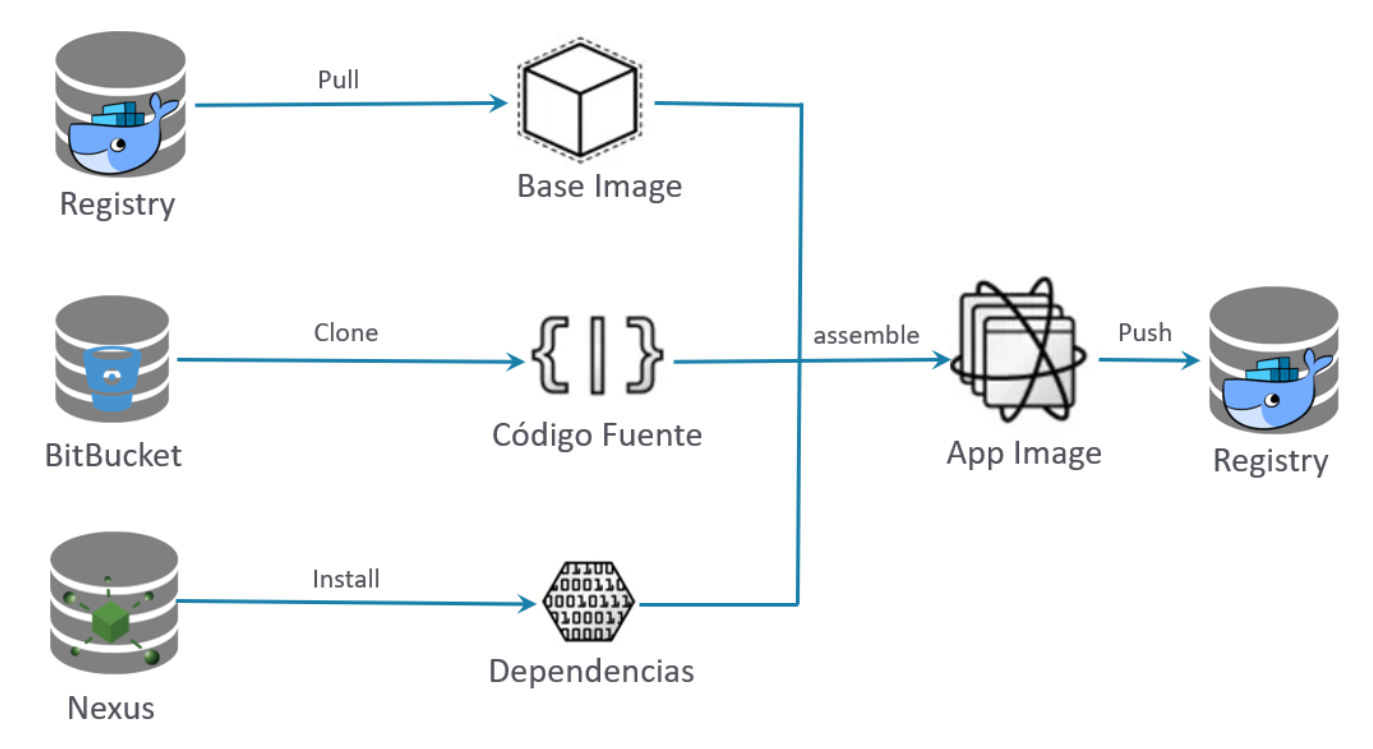
\includegraphics[width=1\textwidth]{images/cont/s2i}
	\caption{S2I en Openshift}
	\label{fig:ocp-s2i}
\end{figure}

La opción más simple para tener una imagen con nuestro código sería generarlas de forma individual y subirlas al repositorio de imágenes de la plataforma, sin embargo esta tarea se volvería algo tediosa conforme el número de servicios crezca, además presentaría dificultades en su mantenimiento y en su integración (como veremos más adelante) con flujos de integración y despliegue continuos. Es por eso que utilizaremos una característica de \textit{OCP} denominada \textit{S2I} (\textit{Sorce to Image}), que nos permitirá a partir de una imagen base (a partir de ahora imagen S2I) generar una nueva imagen personalizada con nuestra aplicación. En la figura \ref{fig:ocp-s2i}.

El proceso de crear la imagen de nuestra aplicación a partir de una imagen S2I y nuestro código o binarios se denomina \textit{Build} y al igual que con la configuración de despliegue para los despliegues \textit{Openshift}, nos proporciona una configuración de \textit{Build} para controlar las versiones y los cambios que se realizan en un mismo tipo de \textit{Build}. A continuación veremos como hemos abordado los casos de \textit{Kafka Streams} y \textit{Tensorflow Serving}.


\subsection{\textit{Kafka Streams}}

En este caso tenemos dos opciones a la hora de crear nuestra imagen de aplicación mediante S2I, partir del código fuente o partir de un binario (un jar generado a partir del código fuente). Hemos optado por esta segunda opción para dejar la compilación y tests fuera de la plataforma \textit{OCP}. 

La imagen \textit{S2I} utilizada es la imagen oficial proporcionada por RedHat para Java. Y a continuación podemos ver como quedaría nuestra configuración de \textit{Build}:

\begin{minted}[
 	gobble=0,
 	frame=single,
 	linenos]{yaml}
apiVersion: build.openshift.io/v1
kind: BuildConfig
metadata:
  labels:
    app: tfm-mgm
  name: topic-model-streaming
  namespace: nbia-prod
spec:
  failedBuildsHistoryLimit: 5
  output:
    to:
      kind: ImageStreamTag
      name: 'topic-model-streaming:latest'
  runPolicy: Serial
  source:
    binary: {}
    type: Binary
  strategy:
    sourceStrategy:
      from:
        kind: ImageStreamTag
        name: 'redhat-openjdk18-openshift:1.4'
        namespace: openshift
    type: Source
  triggers: []
\end{minted}

Algunos aspectos relevantes de la configuración de \textit{Build} son:

\begin{itemize}
\item \textit{\textbf{output}} (línea 10): Nos indica la imagen destino de aplicación que se creará. En nuestro caso la imagen es común ya que todas las clases están embebidas en un mismo binario, por eso posee un valor fijo, pero podría tener un valor variable. La imagen destino debe estar definida en la plataforma. 

\item \textit{\textbf{from}} (línea 20): La imagen \textit{S2I} que se utilizará para crear la imagen de aplicación.

\item \textit{\textbf{triggers}} (línea 25): Al tratarse de un \textit{S2I} binario no existen disparadores por lo que el \textit{Build} debe iniciarse de forma externa proporcionando los binarios.
 
\end{itemize}


\subsection{\textit{Tensorflow Serving}}

En este caso no tenemos elección entre realizar el \textit{build} con fuente o binario, debido a que los modelos que tenemos de \textit{Tensorflow} son binarios. La aproximación, por tanto, será la misma que en el apartado anterior. 

Sin embargo, en este caso no existe ninguna imagen oficial S2I para \textit{Tensorflow Serving} por lo que nos hemos visto obligados a crear nuestra propia imagen S2I a partir de la imagen oficial de \textit{docker} de \textit{Tensorflow Serving}.

El proceso de creación de una imagen S2I consta, a grandes rasgos, de los siguientes pasos: 

\begin{itemize}
\item \textit{Assemble}: Crear los scripts necesarios para una vez recibido los ficheros, colocarlos en la ruta adecuada y construir con ellos la imagen de aplicación. 
\item \textit{Run}: Establecer como debe comportarse la imagen de aplicación.
\item \textit{Usage}: Recopilar el modo de uso de la imagen S2I. 

\end{itemize}








\part{Conclusiones: mantenimiento y futuros trabajos }
\chapter{DevOps}
\label{chapter:mant}

Una vez hemos llegado a esta parte del documento ya hemos realizado el análisis completo de los datos y hemos dejado el modelo en un entorno productivo clasificando llamadas en \textit{real-time}; sin embargo sería muy atrevido dar el proyecto por finalizado.

Probablemente surgirán nuevos datos, dispondremos de nuevas etiquetas, nuestro \textit{software} se degradará, crearemos nuevos y mejores modelos con ideas más o menos brillantes, etc. Este universo cambiante provocará a que se modificarán y/o se crearán nuevos \textit{software} y modelos con bastante frecuencia que será necesario llevar de nuevo a producción.  

Este capítulo tiene objetivo definir los mecanismos y la metodología que hemos establecido para poder reaccionar con gran agilidad ante el cambio, algo esencial hoy en día. En la sección \ref{section:mant:devops} haremos una introducción a la metodología DevOps que acuñaremos en nuestro proyecto, posteriormente pondremos foco en algunos aspectos importantes: La degradación del modelo (sección \ref{section:mant:efi}) y la integración y el despliegue continuos (sección \ref{section:mant:cicd}).


\section{Introducción DevOps}
\label{section:mant:devops}


\begin{figure}[!ht]
	\centering
	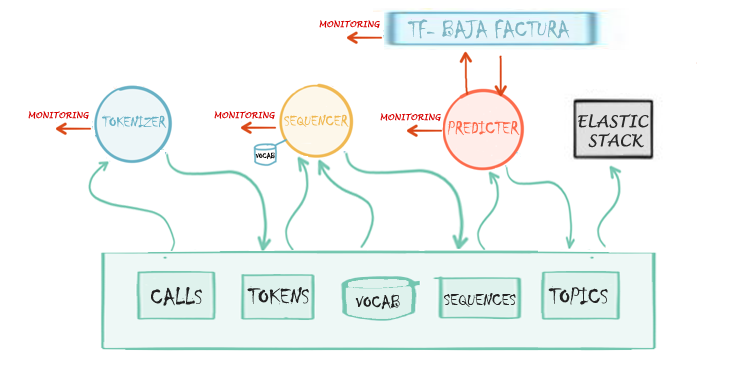
\includegraphics[width=1\textwidth]{images/exp/micro-arch-v3}
	\caption{Arquitectura microservicios}
	\label{fig:micro-arch}
\end{figure}

\section{Degradación del modelo}
\label{section:mant:efi}
Aunque el \textit{software} desarrollado también es propenso de degradarse con el paso del tiempo, si hay algo que tenemos seguro que se va a degradar en este universo cambiante es el modelo. Nuestro modelo se alimenta con las transcripciones de los clientes que están basadas en el servicio que ofrecemos en cada momento, en las inquietudes de nuestros clientes y otros muchos factores externos que pueden influir en la temática de las conversaciones que recibimos.

La certeza en la degradación de nuestro modelo hace que tengamos monitorizar constantemente el rendimiento del mismo, en el caso del modelo supervisado que hemos llevado a producción nos lleva a seguir testeándolo constantemente introduciendo en el flujo llamadas de control etiquetadas para medir su eficiencia.  




\section{Integración y despliegue continuos}
\label{section:mant:cicd}
\chapter{Conclusiones y trabajos futuros}
\label{chapter:conclusiones}

Este último capítulo del documento tiene como objetivo establecer las conclusiones tras la realización de proyecto y enumerar posibles vías de trabajo futuras que permitan darle continuidad al trabajo presentado.

En el apartado \ref{section:con:obj} analizaremos el cumplimiento de los objetivos propuestos al inicio del proyecto. A continuación, en el apartado \ref{section:con:master} veremos como las asignaturas cursadas  a lo largo del máster han contribuido a la realización de este trabajo.  Posteriormente, en los apartados \ref{section:con:fut} y \ref{section:con:neg} trataremos las líneas de trabajo futuras de un modo más general y profundizando en un caso de negocio particular respectivamente. Por último, en el apartado \ref{section:con:fin} abordaremos el resto de conclusiones al margen de los objetivos propuestos. 




\section{Cumplimiento de objetivos}
\label{section:con:obj}

Al empezar este documento, en la sección \ref{section:intro:objetivos}, propusimos una serie de objetivos específicos a cumplir a lo largo del mismo y ahora, una vez finalizado el trabajo, es el momento de evaluar el cumplimiento de los mismos: 

\begin{CheckList}{Goal}
\Goal{achieved}{ \textbf{Construir un modelo que nos permita extraer la temática de las llamadas} a partir de su transcripción a texto. Este objetivo a sido abordado durante la segunda parte del documento que trata el modelado de los datos. Hemos logrado construir tanto modelos no supervisados como supervisados que nos permiten clasificar correctamente las llamadas. En el caso de los modelos supervisados, hemos obtenido varios con precisiones alrededor del 80\% lo que nos permite superar el objetivo propuesto.}
	
\Goal{achieved}{ Desarrollar un mecanismo que nos permita \textbf{extraer esta temática para nuevas llamadas en tiempo real}. Se ha construido usando un inyector que simula las llegadas de llamadas en tiempo real. El desarrollo del objetivo usando una arquitectura de microservicios puede verse en el capítulo \ref{chapter:prod} dedicado a la capa de \textit{streaming}.
}	

\Goal{achieved}{  Disponer de una\textbf{ visualización en tiempo cuasi real} para que pueda visualizarse la evolución de las temáticas a lo largo del tiempo. Se ha logrado disponer de visualizaciones en tiempo real que muestran la información de las clasificaciones hechas por nuestro modelo. El desarrollo de estas visualizaciones ha sido tratado en el capítulo \ref{chapter:servicio}.

}

\Goal{achieved}{  Proporcionar un \textbf{sistema de alertado} que nos permita detectar anomalías en el número de llamadas que se reciben de un determinado tema. Se han creado alertas dinámicas capaces de detectar anomalías en serie temporales, en nuestro caso usando el número de llamadas que se reciben por cada tema a lo largo del tiempo. El cumplimiento de este objetivo se encuentra detallado en el capítulo  \ref{chapter:servicio}.
}

\end{CheckList}

El cumplimiento de estos objetivos ha sido prácticamente total, aunque la precisión de los modelos supervisados esté en el 80\% ha sido complementado con la creación de modelos no supervisados. En cuanto al resto de objetivos estos han sido cubiertos al 100\%.





\section{Aplicación máster}
\label{section:con:master}
Aunque se ha profundizado en algunos aspectos más allá de lo aprendido a lo largo del máster, las asignaturas cursadas a lo largo de tres semestres han creado una base sólida que ha permitido el desarrollo de este proyecto.

En esta sección queremos hacer un repaso sobre la aplicación que todas las asignaturas cursadas a lo largo del máster, en mayor o menor medida, han tenido en este proyecto. 

\begin{itemize}

\item \textbf{Fundamentos de la ciencia de datos}: Esta asignatura nos ha permitido entender los principios básicos del mundo de la ciencia de datos. Entre otros aspectos, la hemos utilizado para entender el ciclo de vida de un proyecto de ciencia de datos. También se han tratado otros aspectos que nos han sido útiles en el desarrollo del proyecto, como son la metodología \textit{Agile}, la calidad de los datos, etc.

\item \textbf{Tipología y ciclo de vida de los datos}: Esta asignatura es fundamental para entender el ciclo de vida de los datos. En ella hemos tratado los diferentes tipos de datos que podemos encontrar y las formas que tenemos de obtenerlos.

\item \textbf{Arquitecturas de bases de datos no tradicionales}: En esta asignatura se trabajó con diferentes  modelos de bases de datos NoSQL que han sido fundamentales para el desarrollo del proyecto. En nuestro proyecto hemos trabajados con \textit{Elasticsearch} en la capa de servicio, que aunque se trate de un motor de búsqueda, presenta muchas similitudes con una BBDD NoSQL documental. Además se ha trabajado en la capa de \textit{streaming} con Apache Kafka que interiormente posee una BBDD RocksDB, que se trata de una NoSQL clave-valor. 

\item \textbf{Estadística avanzada}: Aunque no se han aplicado los modelos estadísticos vistos en esta asignatura, han  sido útiles los conceptos vistos para las fases de preprocesado y análisis de los datos.



\item \textbf{Minería de datos}: En esta asignatura se trabajaron a nivel práctico los métodos \textit{core} de la minería de datos. Para nuestro proyecto han sido de utilidad conceptos de preparación de datos, de \textit{clustering} y de evaluación de modelos. 

\item \textbf{Modelos avanzados de minería de datos}: En esta asignatura se profundiza más en los modelos de minería de datos y empezamos a aplicar las redes neuronales, que son la base de nuestros modelos supervisados, además tratamos temas que nos han sido útiles como la combinación de clasificadores.


\item  \textbf{Deep learning}: El contenido de esta asignatura ha sido vital para los modelos de aprendizaje supervisado. En ella hemos profundizado en el mundo de las redes neuronales y los diferentes tipos: convolucionales, recurrentes, etc.

\item  \textbf{Análisis de sentimientos y redes sociales}: En esta asignatura se trabajaron las bases del procesamiento del lenguaje natural que ha sido el \textit{core} de nuestro proyecto.

\item  \textbf{Visualización de datos}: En esta asignatura trabajamos los conceptos que existen detrás de una buena visualización. Estos conceptos se han intentado aplicar en nuestro proyecto, tanto en la fase de análisis como en la capa de servicio y visualización. Las visualizaciones interactivas se han creado en nuestro caso a través de Kibana.

\item  \textbf{Diseño y construcción del data warehouse}: Aunque no se han aplicado directamente los conocimientos de esta asignatura en el desarrollo del proyecto, sí ha sido necesario acceder al \textit{datawarehouse} de la empresa para la obtención de datos.


\item \textbf{Análisis de datos en entornos big data}: Aunque sin cursar esta asignatura, hemos aplicado algunos conceptos tratados en ella y relacionados con el uso de un ecosistema Hadoop. Principalmente HDFS, Spark y Hive.


\end{itemize}





\section{Líneas de trabajo futuras}
\label{section:con:fut}

Una vez finalizado el proyecto es el momento de abrir líneas de trabajos futuros que le den continuidad al trabajo aquí expuesto, ya sea ampliando su alcance o mejorando algunos aspectos.




\begin{itemize}
	\item \textbf{Métricas Optimización}: Modificar las métricas usadas para la evaluación, usando por ejemplo F1-score que nos proporcionará una mejor medida de los casos clasificados incorrectamente que la métrica de precisión utilizada.
	\item \textbf{Etiquetas monitorización}: Como hemos visto a lo largo del documento, principalmente en el capítulo \ref{chapter:dataset}, las etiquetas que tienen más calidad son las de monitorización, aunque tenían el problema del escaso porcentaje de etiquetas de este tipo. En un futuro se espera que el porcentaje de llamadas etiquetadas de este tipo aumente, pudiéndose aplicar los modelos vistos a estos datos.
	\item \textbf{Etiquetas de sistemas operacionales}: Una opción que no se ha abordado hasta ahora es la de etiquetar las llamadas en función de las operaciones hechas por los clientes tras las llamadas. Por ejemplo si han realizado un alta, si han realizado una baja, si han abierto una reclamación, etc. Estas acciones pueden consultarse directamente en los sistemas operacionales de la empresa.
	\item \textbf{Llevar a producción modelo no supervisado}: Aunque se ha realizado un estudio no supervisado de las llamadas, este no se ha llevado a un entorno productivo. Puede ser muy interesante introducir un modelo no supervisado en nuestra arquitectura para tener en la capa de servicio una versión distinta a la de las etiquetas actuales. 
	\item \textbf{Adaptar llamadas tiempo real, eliminar inyector}: En este proyecto se ha presentado un elemento que simula las llamadas en tiempo real, a corto plazo será necesario eliminar este elemento y adaptar los datos de entrada del servicio \textit{tokenizer} a los datos reales de las llamadas. 
	
	\item \textbf{Ciclo DevOps completo}: Aunque hemos dedicado un capítulo completo \ref{chapter:mant} a la metodología DevOps, se trata de un proyecto realizado de forma individual, en el momento en el que dispongamos de diferentes entornos (por ejemplo desarrollo, certificación y producción) y existan diferentes equipos trabajando en el proyecto será el momento de establecer el ciclo completo DevOps trabajando aspectos como el despliegue entre entornos, la comunicación entre equipos o las pruebas \textit{end-to-end} en un entorno aislado.
	
	
	\item \textbf{Otras funcionalidades}: Tanto la arquitectura expuesta en la capa de \textit{streaming}, como la capa de servicio pueden ser usadas para dotar al sistema de otras capacidades relacionadas con el modelo. Algunas de las funcionalidades que pueden ser útiles para complementar el sistema son: el análisis de sentimientos, analizar si una llamada ha supuesto una venta positiva, etc. 


\end{itemize}

En resumen, pensamos que se trata de un trabajo con mucho recorrido y margen de mejora y esperamos que este proyecto posea continuidad en el futuro.

\section{Caso de negocio}
\label{section:con:neg}

Aunque hemos dedicado la sección anterior en enumerar posibles líneas de trabajo futuras, queremos esbozar en este apartado un posible caso de negocio en el que un proyecto de este tipo encajaría y aportaría valor a la empresa. 

Las personas encargadas de recibir las llamadas en un \textit{call center} deben de atender a un gran número de llamadas de diferente tipología. En función del tipo de llamada, lo ideal es disponer de un tipo de agente especializado en la temática a resolver. Vamos a ver algunos ejemplos de tipos de llamadas que pueden requerir diferentes agentes:

\begin{itemize}
\item \textbf{Consulta}:  Los clientes que realicen consultas sobre diferentes productos, lo ideal es que sean atendidos por agentes especializados en la venta. Deben ser capaces de conseguir que aumente el interés del cliente por nuestros productos hasta el punto de generar una contratación. 

\item \textbf{Reclamación Facturación}: Un porcentaje representativo de las llamadas se realiza para la reclamación de diferentes aspectos relacionados con la facturación. Las resoluciones de este tipo de llamadas están acotadas y  no es necesario un gran \textit{expertise} por parte del agente. 

\item \textbf{Baja}: De las labores realizadas por los agentes telefónicos, quizás una de las labores más difíciles y que más valor aporta a la empresa, es la de evitar que una baja se produzca cuando un cliente llama convencido de efectuarla. Tener buenos agentes atendiendo este tipo de tareas repercute directamente en el beneficio de la empresa provocando una disminución del \textit{churn}.
\end{itemize}



Estos tipos de llamada y de agentes nos servirán de ejemplo para mostrar los beneficios que la clasificación automática de llamadas puede tener para la empresa, más allá de lo comentado en el documento.

Es lógico pensar que los agentes especializados en realizar nuevas ventas y los agentes encargados de evitar las bajas tendrán un coste mayor que, por ejemplo, los agentes encargados de realizar las reclamaciones de facturación que realizan labores más mecánicas. Esta variación en el coste y el objetivo de poder ofrecer una mejor calidad de servicio, haciendo que cada agente solo responda las llamadas que mejor puede resolver, pone de manifiesto la importancia de realizar una buena clasificación previa. 

Una de nuestras propuestas a futuro es la posibilidad de usar un sistema de este tipo para realizar la clasificación de la llamada a partir de una descripción del cliente, mejorando el sistema en el que el cliente realiza la clasificación mediante un menú y opciones. Este sistema además podría combinarse con un asistente virtual con capacidades cognitivas permitiendo a un sistema de este tipo ser incluso más ambicioso y ser autónomo para las tareas más ambiciosas (como la reclamación de facturas).

Un proyecto de este tipo se traduciría en los siguientes beneficios: 

\begin{itemize}
\item \textbf{Reducción del tiempo de atención del agente}, al recibir unicamente llamadas para las que se encuentra especializado. Los agentes de un \textit{call center} tienen una penalización por llamadas largas. 
\item \textbf{Mejora del FCR} ( \textit{First Call resolution}) debido a que los agentes tratarán un número de temas más reducido y de los que tienen un mayor control. Actualmente se otorgan incentivos a los agentes por evitar que se produzca una segunda llamada, del 25\% aproximadamente del coste de la llamada. 
\item Posibilidad de automatizar las llamadas ``más mecánicas'' al poder clasificarlas y aislarlas, disminuyendo la necesidad de agentes. 

\item \textbf{Reducción del \textit{churn}} al mejorar el porcentaje de las llamadas de baja que son atendidas por agentes especializadas.

\item \textbf{Mejora del CEX} (\textit{Customer EXperience}) al recibir el cliente una mejor atención especializada.



\end{itemize}

Con los cuatro primeros puntos, al ser beneficios cuantitativos, sería bastante factible generar un caso de negocio que justificara la realización de un proyecto de este tipo. El quinto representaría un valor intangible, fundamental para una empresa y reforzaría la propuesta.



\section{Conclusiones finales}
\label{section:con:fin}

Más allá de la valoración del cumplimiento de los objetivos propuestos y de las futuras líneas de trabajo que abrimos queremos finalizar el trabajo extrayendo una serie de conclusiones del mismo. 


\begin{itemize}
\item El trabajo con datos reales ha supuesto todo un reto. La falta de calidad de los mismos en determinados momentos, el hecho de tener que enriquecerlos con otras fuentes de datos, la necesidad de filtrar y limpiar ha añadido una dificultad extra al proyecto que si hubiera sido en un entorno controlado con datos ``prefabricados''. También ha sido una experiencia gratificante obtener algo de valor de datos reales. 

\item La creación de modelos en un proyecto real es un proceso que puede requerir una gran cantidad de tiempo y ``siempre'' es posible afinar un poco más un modelo. Esto nos ha hecho darnos cuenta de que es importante fijarse unos objetivos factibles y establecer un punto de parada.

\item El buen rendimiento de modelos con redes neuronales recurrentes para la clasificación de textos y el elevado coste de entrenamiento que estos tienen. 

\item La importancia de la representación elegida para las transcripciones y el buen funcionamientos de los modelos Word2Vec.

\item El aprendizaje no supervisado es un proceso que requiere una gran capacidad de análisis por nuestra parte ya que no siempre obtenemos lo que esperamos y es necesario descubrir los patrones encontrados por los modelos.

\item Este proyecto nos ha hecho darnos cuenta de las amplias posibilidades del aprendizaje profundo, pero también de la gran cantidad de datos que necesitamos normalmente para entrenar estos modelos. Esto no ha llevado a tener que prescindir de momento de algunas etiquetas debido a su escasez.  

\item El entrenamiento de los modelos supervisados nos ha hecho también enfrentarnos en la realidad a varios problemas vistos a lo largo del máster como son el sobrentrenamiento y las clases desbalanceadas. 

\item Durante este proyecto hemos tenido la posibilidad de trabajar con GPUs, poniendo de manifiesto la gran capacidad de este tipo de \textit{hardware} para entrenar modelos de aprendizaje profundo. Sin embargo, se ha demostrado que estos modelos, una vez entrenados, pueden tener un rendimiento bastante decente sobre plataformas de con CPUs.



\item El trabajo expuesto expone una implementación real de la arquitectura Kappa llevando al terreno práctico las ideas propuestas por Jay Kreps. Además incorpora a esta arquitectura los modelos de aprendizaje profundo creados con Tensorflow. 

Creemos que más allá de la clasificación de llamadas, esta propuesta puede ser de utilidad a la hora de dar el salto ``del laboratorio'' a la producción; ayudando a desplegar otros modelos productivos dentro de la empresa reaprovechando las capacidades creadas tanto en la capa de \textit{streaming} como en la capa de servicio.    

\item Otra de las aportaciones que creemos que este trabajo realiza a la empresa es la aproximación que se ha hecho a la metodología DevOps permitiendo que toda la arquitectura sea factible de entrar en un ciclo de integración y despliegue continuos, siendo algo reutilizable para cualquier otro nuevo proyecto que use esta misma arquitectura. 

\item Pensamos que otra de las partes reutilizables de este trabajo es el esfuerzo realizado para la monitorización de todos los procesos Kafka Streams y Tensorflow Serving. Esta tarea se ha realizado de modo que sea totalmente reaprovechable por otros procesos de estas tecnologías. Teniendo la posibilidad de obtener datos del rendimiento y del uso de recursos de los mismos y las visualizaciones y alertas necesarias para controlarlo.

\item Por último, uno de los retos que hemos asumido en este proyecto es que el despliegue de toda la parte productiva se haga sobre contenedores. Además esta tarea se ha realizado de modo que sean reutilizables por futuras aplicaciones gracias a S2I.
\end{itemize}






 

%Apendices
%\begin{appendices}
%\chapter{Módulo Python mgmtfm}
%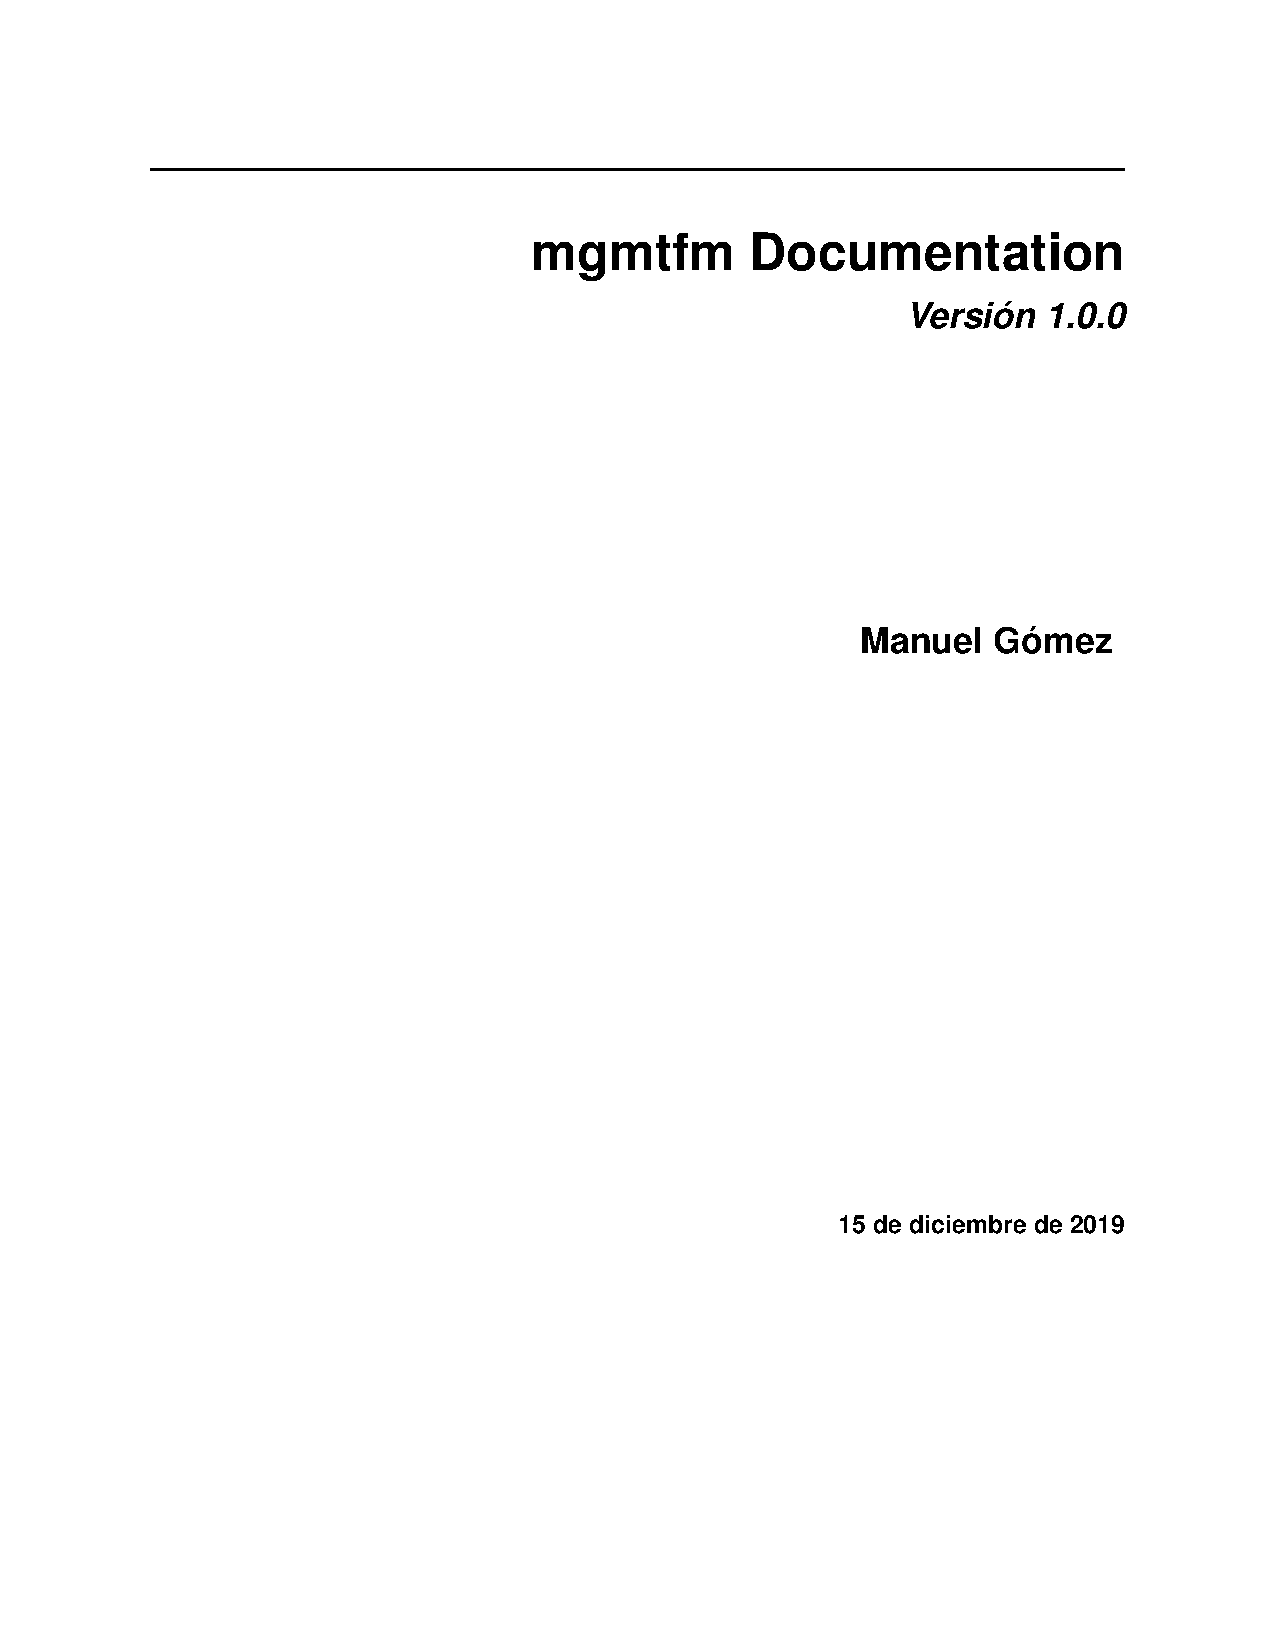
\includepdf[pages=-]{appendices/mgmtfm.pdf}
%\end{appendices}


% bibliografia
\addcontentsline{toc}{chapter}{Bibliografía}
\bibliographystyle{plain}
\bibliography{referencias}


%\newpage

%\appendix
%\addcontentsline{toc}{chapter}{Appendix}
%\addtocontents{toc}{\protect\contentsline{chapter}{Appendix:}{}}
%\chapter{mgmpdf}
%



\end{document}